% !TEX TS-program = pdflatex
% !TEX encoding = UTF-8 Unicode

\documentclass[11pt]{report} % use larger type; default would be 10pt

\usepackage[utf8]{inputenc} % set input encoding (not needed with XeLaTeX)
\usepackage[czech]{babel}

%%% PAGE DIMENSIONS
\usepackage{geometry} % to change the page dimensions
\geometry{a4paper} % or letterpaper (US) or a5paper or....
\geometry{top=45 px, left=65px,right=65px,bottom=55px} % for example, change the margins to 2 inches all round

\usepackage{graphicx} % support the \includegraphics command and options
\usepackage{hyperref}
\usepackage{indentfirst}
\usepackage{float}
\usepackage{listings}
\usepackage{xfrac}
\usepackage{amsmath, amsthm, amssymb}
\usepackage{mathtools}
\usepackage{array}
\usepackage{caption}
\usepackage{enumitem}
\usepackage{algorithm}
\usepackage[noend]{algpseudocode} 
\usepackage{titlesec}

\setcounter{secnumdepth}{4}
\setcounter{tocdepth}{4}
\titleformat{\paragraph}
{\normalfont\normalsize\bfseries}{\theparagraph}{1em}{}
\titlespacing*{\paragraph}
{0pt}{3.25ex plus 1ex minus .2ex}{1.5ex plus .2ex}
\titleformat{\subparagraph}
{\normalfont\normalsize\bfseries}{\theparagraph}{0.5em}{}
\titlespacing*{\subparagraph}
{0pt}{3.25ex plus 1ex minus .2ex}{1.5ex plus .2ex}

\setlist{noitemsep}
\setlist[1]{leftmargin=50pt}
\setlist[description, 1]{labelindent=20pt}
%\setlist[1]{labelindent=\parindent} % < Usually a good idea

%\setlist[enumerate]{labelsep=*, leftmargin=1.5pc}


\newcommand{\R}{\mathbb{R}}
\newcommand{\N}{\mathbb{N}}
\renewcommand{\vec}[1]{\mathbf{#1}}

\newtheorem{theorem}{Věta}[section]
\newtheorem{implication}{Důsledek}[section]

\numberwithin{equation}{section}

\makeatletter
\newcommand{\dotminus}{\mathbin{\text{\@dotminus}}}

\newcommand{\@dotminus}{%
	\ooalign{\hidewidth\raise1ex\hbox{.}\hidewidth\cr$\m@th-$\cr}%
}
\makeatother

\lstset
{ %Formatting for code in appendix
	numbers=left,
	stepnumber=1,
	tabsize = 4
}
\usepackage{wrapfig}

%%% The "real" document content comes below...


\begin{document}
	
\tableofcontents
\part{Společné povinné okruhy}
\chapter{Základy složitosti a vyčíslitelnosti}
\section{Výpočetní modely (Turingovy stroje, RAM).}
\subsection{Turingův stroj}
\textbf{(Jednopáskový deterministický) Turingův stroj (TS)} $M$ je pětice
$$M = (Q, \Sigma, \delta, q_0, F)$$
\begin{itemize}
	
	
	\item $Q$ je konečná \textbf{množina stavů}.
	\item $\Sigma$ je konečná \textbf{pásková abeceda}, která obsahuje znak $\lambda$ pro prázdné políčko. (Často budeme rozlišovat \textbf{páskovou (vnitřní)} a \textbf{vstupní (vnější) abecedu}.)
	\item $\delta : Q \times \Sigma \mapsto Q \times \Sigma \times \{R, N, L\} \cup {\bot}$ je \textbf{přechodová funkce},
	kde $\bot$ označuje nedefinovaný přechod.
	\item $q_0 \in Q$ je \textbf{počáteční stav}.
	\item $F \subseteq Q$ je \textbf{množina přijímajících stavů}.
\end{itemize}

Turingův stroj sestává z \textbf{řídící jednotky}, \textbf{pásky}, která je potenciálně nekonečná v obou směrech, a
\textbf{hlavy} pro čtení a zápis, která se pohybuje oběma směry.

\textbf{Displej} je dvojice $(q, a)$, kde $q \in Q$ je aktuální stav Turingova stroje a $a \in \Sigma$ je symbol pod hlavou. Na základě displeje TS rozhoduje, jaký další krok má vykonat.

\textbf{Konfigurace} zachycuje stav výpočtu Turingova stroje a skládá se ze
\begin{itemize}
	
	
	\item stavu řídící jednotky
	\item slova na pásce (od nejlevějšího do nejpravějšího neprázdného políčka)
	\item pozice hlavy na pásce (v rámci slova na této pásce)
\end{itemize}

\subsubsection{Výpočet TS}
\textbf{Výpočet} zahajuje TS $M$ v \textbf{počáteční konfiguraci}, tedy v počátečním stavu se vstupním slovem zapsaným na pásce a hlavou nad nejlevějším symbolem vstupního slova. Vstupní slovo nesmí obsahovat prázdné políčko. Pokud se $M$ nachází ve stavu $q \in Q$ a pod hlavou je symbol $a \in \Sigma$, pak krok výpočtu probíhá následovně:
\begin{enumerate}
	
	
	\item Je-li $\delta(q, a) = \bot$, výpočet $M$ končí,
	\item Je-li $\delta(q, a) = (q', a', Z)$, kde $q' \in Q$, $a' \in \Sigma$ a $Z \in \{L, N, R\}$, přejde $M$ do stavu $q'$, zapíše na pozici hlavy symbol $a'$ a pohne hlavou doleva (pokud $Z = L$), doprava (pokud $Z = R$), nebo hlava zůstane stát (pokud $Z = N$).	
\end{enumerate}

TS $M$ \textbf{přijímá slovo} $w$, pokud výpočet $M$ se vstupem $w$ skončí a $M$ se po ukončení výpočtu nachází v přijímajícím stavu. 

TS $M$ \textbf{odmítá slovo} $w$, pokud výpočet $M$ nad vstupem $w$ skončí a $M$ se po ukončení výpočtu nenachází v přijímajícím stavu. 

Fakt, že výpočet $M$ nad vstupním slovem $w$ skončí, označíme pomocí $M(w){\downarrow}$ a řekneme, že výpočet \textbf{konverguje}. 

Fakt, že výpočet $M$ nad vstupním slovem $w$ nikdy neskončí, označíme pomocí $M(w){\uparrow}$ a řekneme, že výpočet \textbf{diverguje}.

\subsubsection{Turingovsky rozhodnutelné jazyky}
\textbf{Jazyk slov přijímaných} TS $M$ označíme pomocí $L(M)$. 

Řekneme, že jazyk $L$ je \textbf{částečně (Turingovsky) rozhodnutelný} (též \textbf{rekurzivně spočetný}), pokud existuje
Turingův stroj $M$, pro který $L = L(M)$.

Řekneme, že jazyk $L$ je \textbf{(Turingovsky) rozhodnutelný} (též \textbf{rekurzivní}), pokud existuje Turingův stroj $M$, který se \textit{vždy zastaví} a $L = L(M)$.

\subsubsection{Turingovsky vyčíslitelné funkce}
Turingův stroj $M$ s páskovou abecedou $\Sigma$ \textbf{počítá} nějakou \textit{částečnou} funkci $f_M : \Sigma^* \mapsto \Sigma^*$ (částečná = pro některé vstupy není definovaná). Pokud $M(w){\downarrow}$ pro daný vstup $w \in \Sigma^*$, je hodnota funkce $f_M(w)$ \textbf{definovaná}, což označíme pomocí $f_M(w){\downarrow}$. \textbf{Hodnotou funkce} $f_M(w)$ je potom slovo na (výstupní) pásce $M$ po ukončení výpočtu nad $w$. Pokud $M(w){\uparrow}$, pak je hodnota $f_M(w)$ \textbf{nedefinovaná}, což označíme pomocí $f_M(w){\uparrow}$. 

Funkce $f : \Sigma^* \mapsto \Sigma^*$ je \textbf{turingovsky vyčíslitelná}, pokud existuje Turingův stroj \textbf{M}, který ji počítá. \textbf{\textit{Každá turingovsky vyčíslitelná funkce má nekonečně mnoho různých Turingových strojů, 	které ji počítají!}}

\subsubsection{Varianty TS}
Turingovy stroje mají řadu variant, například:
\begin{itemize}
	
	
	\item TS s jednosměrně nekonečnou páskou
	\item TS s více páskami (vstupní/výstupní/pracovní)
	\item TS s více hlavami na páskách
	\item TS s pouze binární abecedou
	\item nedeterministické TS
\end{itemize}
Zmíněné varianty jsou ekvivalentní \uv{našemu} modelu v tom smyslu, že všechny přijímají touž třídu jazyků a vyčíslují touž třídu funkcí.

\textbf{$k$-páskový Turingův stroj} se od jednopáskového Turingova stroje líší následujícím způsobem:
\begin{itemize}
	
	
	\item Má $k$ pásek, na každé je zvláštní hlava.
	\begin{itemize}
		
			
		\item Vstupní páska na počátku obsahuje vstupní řetězec. Často je určena jen pro čtení.
		\item Pracovní pásky jsou určeny pro čtení i zápis.
		\item Výstupní páska na konci obsahuje výstupní řetězec. Často je určena jen pro zápis s pohybem hlavy jen vpravo.
	\end{itemize}
	\item Hlavy na páskách se pohybují nezávisle na sobě.
	\item Přechodová funkce je typu
		$$\delta : Q \times \Sigma^k \mapsto Q \times \Sigma^k \times \{R, N, L\}^k \cup {\bot}$$
\end{itemize}

Neplést \textit{multi-tape (vícepáskové)} a \textit{multi-track} TS. Druhé jmenované mají také více pásek, ale \textit{jedinou hlavu společnou pro všechny}.

\begin{theorem}
Ke každému $k$-páskovému Turingovu stroji $M$ existuje jednopáskový Turingův stroj $M'$, který simuluje práci $M$, přijímá týž jazyk jako $M$ a počítá touž funkci jako $M$.
\end{theorem}
\begin{proof}
	Pouze idea. Chceme simulovat $k$-páskový na jednopáskovém. Dvě varianty:
	\begin{enumerate}
		
		
		\item Obsahy pásek zapíšeme na jedinou, oddělíme je novým symbolem $\#$. Pozice hlav označuje speciální značka, např. je-li hlava nad symbolem $0$, označíme to pomocí $\overline{0}$ -- v praxi to znamená pro každý symbol přidat do abecedy jeho označkovanou variantu, tj. $|\Sigma|$ nových symbolů. Dojde-li nějaké pásce místo, musí se všechny symboly vpravo od ní posunout.
		
		\item Vytvoříme novou abecedu $\Sigma'$ jako kartézský součin $k$ abeced, tj. $\Sigma' = \Sigma^k$. Jeden symbol tedy reprezentuje $k$-tici původních symbolů. Je taky potřeba ošetřit pozici hlav.
	\end{enumerate}
\end{proof}

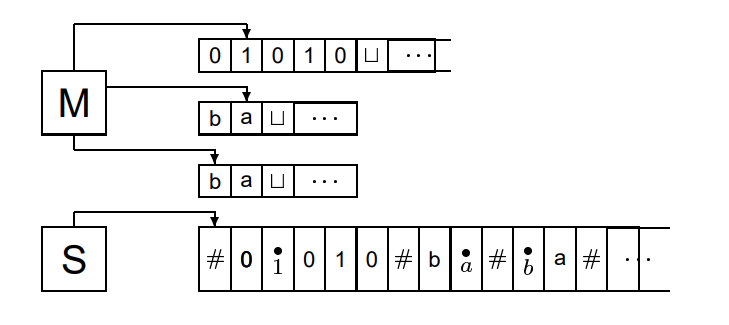
\includegraphics[width=0.6\textwidth]{img/turing_multi_seq.png}

\subsection{RAM (Random Access Machine)}
\begin{wrapfigure}{r}{0.4\textwidth}
	\centering
	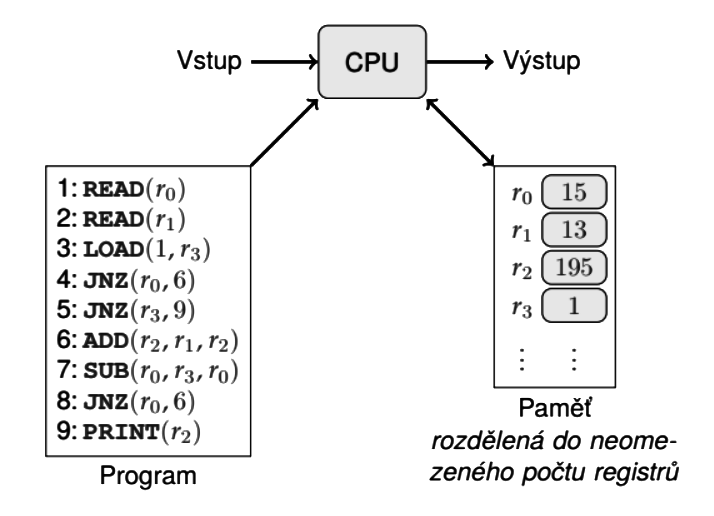
\includegraphics[width=0.35\textwidth]{img/ram.png}
\end{wrapfigure}
RAM je stroj s náhodným přístupem do paměti. Jde o model, který se často používá jako základní výpočetní model při měření časové i prostorové složitosti algoritmů. Cílem bylo vytvořit model, který by se co nejvíce blížil reálným počítačům. Podobně jako Turingovy stroje, i RAM je strojem s \textbf{oddělenou pamětí pro data a pro instrukce}, nejedná se tedy o stroje Von Neumannovy architektury. 

\textbf{Program} pro RAM je konečnou posloupností instrukcí $P = I_0, I_1, I_2, \dots I_l$

Paměť pro data se skládá z neomezené posloupnosti registrů $r_i, i \in \mathbb{N}$ Obsahem registru může být libovolně velké přirozené číslo. Při popisu instrukcí budeme dodržovat následující konvence:
\begin{itemize}
	
	
	\item Obsah registru $r_i$ budeme označovat pomocí $[r_i]$.
	\item Nepřímá adresace (tj. obsahem jiného registru) pomocí $[[r_i]] = [r_{[r_j]}]$. 
	\item Přiřazení hodnoty $c$ do registru $r_i$ označíme $r_i \leftarrow c$
\end{itemize}

Seznam instrukcí pro RAM viz tabulka \ref{ram_instrukce}.
\begin{table}[H]
	\centering
	\renewcommand{\arraystretch}{1.5}
	\begin{tabular}{|l|l|}
		\hline
		LOAD($C, r_i$) 			& $r_i \leftarrow C$ 							\\ \hline
		ADD($r_i, r_j, r_k$) 	& $r_k \leftarrow [r_i] + [r_j]$				\\ \hline
		SUB($r_i, r_j, r_k$) 	& $r_k \leftarrow [r_i] \dotminus [r_j]$\quad ($x \dotminus y = max(x-y, 0)$)    	\\ \hline
		COPY($[r_p], r_d$) 		& $r_d \leftarrow [[rp]]$				 		\\ \hline
		COPY($r_s,[r_d]$) 		& $r_{[r_d]} \leftarrow [r_s]$                  \\ \hline
		JNZ($r_i, I_z$) 		& if $[r_i] > 0$ then goto instruction $I_z$ 	\\ \hline
		READ($r_i$) 			& $r_i \leftarrow$ input						\\ \hline
		PRINT($r_i$) 			& output $\leftarrow [r_i]$   					\\ \hline
	\end{tabular}
	\caption{Seznam instrukcí RAM}
	\label{ram_instrukce}
\end{table}

\subsubsection{Jazyky rozhodnutelné RAM}
Uvažme abecedu $\Sigma = \{\sigma_1, \sigma_2, \dots, \sigma_k\}$. Slovo $w = \sigma_{i_1}, \sigma_{i_2} \dots \sigma_{i_n}$ předáme RAMu $R$ jako posloupnost čísel $i_1, \dots, i_n$. Konec slova pozná $R$ díky tomu, že READ načte 0, není-li už k dispozici vstup.

RAM $R$ \textbf{přijme} slovo $w$, pokud $R(w){\downarrow}$ a první číslo, které $R$ zapíše na výstup je 1.

RAM $R$ \textbf{odmítne} slovo w, pokud $R(w){\downarrow}$ a $R$ buď na výstup nezapíše nic, nebo první zapsané číslo je jiné než 1.

\textbf{Jazyk slov přijímaných RAMem} $R$ označíme pomocí $L(R)$. 

Pokud pro jazyk $L$ platí, že $L = L(R)$ pro nějaký RAM, pak řekneme, že je \textbf{částečně rozhodnutelný (RAMem)}. Pokud se navíc výpočet $R$ \textit{nad každým vstupem zastaví}, řekneme, že je $L = L(R)$ \textbf{rozhodnutelný (RAMem)}.

\subsubsection{Funkce vyčíslitelné na RAMu}
O RAMu $R$ řekneme, že \textbf{počítá} částečnou \textit{aritmetickou} funkci $f : \N^n \mapsto \N, n \geq 0$, pokud za předpokladu, že $R$ dostane na vstup $n$-tici $(x_1, \dots, x_n)$, platí následující:
\begin{itemize}
	
	
	\item Je-li $f(x_1, \dots, x_n){\downarrow}$, pak $R(x_1, \dots, x_n){\downarrow}$ a $R$ vypíše na výstup hodnotu $f(x_1, \dots, x_n)$.
	\item Je-li $f(x_1, \dots, x_n){\uparrow}$, pak $R(x_1, \dots, x_n){\uparrow}$.
\end{itemize}
O funkci $f$, pro niž existuje RAM, který ji počítá, řekneme, že je \textbf{vyčíslitelná na RAMu}.

\subsubsection{Řetězcové (string) funkce vyčíslitelné na RAMu}
RAM $R$ \textbf{počítá} částečnou (\textit{řetězcovou}) funkci $f : \Sigma^* \mapsto \Sigma^*$, kde $\Sigma = \{\sigma_1, \sigma_2, \dots, \sigma_k\}$, pokud platí:
\begin{itemize}
	
	
	\item Vstupní řetězec $w = \sigma_{i_1}\sigma_{i_2}\dots\sigma_{i_n}$ je předaný jako posloupnost čísel $i_1, \dots, i_n$.
	\item Konec slova pozná $R$ díky tomu, že READ načte 0, není-li už k dispozici vstup.
	\item Pokud je $f(w){\downarrow}= \sigma_{j_1}\sigma_{j_2}\dots\sigma_{j_m}$, pak $R(w){\downarrow}$ a na výstup je
	zapsaná posloupnost čísel $j_1, j_2, \dots, j_m, 0$.
	\item Pokud $f(w){\uparrow}$, pak $R(w){\uparrow}$.
\end{itemize}
O funkci $f$, pro níž existuje RAM $R$, který ji počítá, říkáme, že je \textbf{vyčíslitelná na RAMu}.

\subsubsection{Programování na RAMu}
Programy pro RAM odpovídají procedurálnímu jazyku:
\begin{itemize}
	
	
	\item Máme k dispozici \textbf{proměnné} (\textbf{skalární} i \textbf{neomezená pole}):
	
	Předpokládejme, že v programu používáme pole $A_1, \dots, A_p$ a skalární proměnné $x_0, \dots, x_s$.
	\begin{itemize}
		
		
		
		\item Pole indexujeme od 0.
		\item Prvek $A_i[j]$, kde $i \in \{1, \dots, p\}, j \in \N$, umístíme do registru $r_{i+j\cdot(p+1)}$.
		\item Prvky pole $A_i, i = 1, \dots, p$ jsou tedy v registrech $r_i, r_{i+p+1}, r_{i+2(p+1)}, \dots$
		\item Proměnnou $x_i$, kde $i \in \{0, \dots, s\}$ umístíme do registru $r_{i\cdot(p+1)}$.
		\item Skalární proměnné jsou tedy postupně v registrech $r_0, r_{p+1}, r_{2(p+1)}, \dots$
	\end{itemize}

	\item Cykly (\textbf{for} i \textbf{while}) – s pomocí podmíněného skoku, případně čítače v proměnné.
	\item Nepodmíněný skok (\textbf{goto}) – s použitím pomocného registru, kam uložíme 1 a použijeme podmíněný skok.
	\item \textbf{Podmíněný příkaz} – s pomocí podmíněného skoku.
	\item \textbf{Funkce a procedury} – do místa použití funkce rovnou v programu napíšeme tělo funkce (inline).
	\item \textit{Nemáme rekurzivní volání funkcí} – ta se však dají vždy nahradit pomocí cyklu while a zásobníku.	
\end{itemize}

\subsubsection{Ekvivalence RAM a TS}
\begin{theorem}
	Ke každému Turingovu stroji $M$ existuje ekvivalentní RAM $R$.
\end{theorem}
\begin{proof}
	Odpovídající RAM sestrojíme takto:
	\begin{itemize}
		
		
		\item Obsah pásky uložen ve dvou polích: $T_r$ obsahuje pravou část pásky a $T_l$ obsahuje levou část pásky.
		\item Poloha hlavy – pamatujeme si index v proměnné $h$ a stranu pásky (pravá/levá) v proměnné $s$.
		\item Stav – v proměnné $q$.
		\item Výběr instrukce – podmíněný příkaz podle $h$, $s$ a $q$		
	\end{itemize}

\end{proof}


\begin{theorem}
Ke každému RAMu $R$ existuje ekvivalentní Turingův stroj $M$.
\end{theorem}
\begin{proof}
	K RAMu $R$ sestrojíme TS $M$ jako 4-páskový:
	\begin{description}
		
		
		
		\item[Vstupní páska] Posloupnost čísel, která má dostat $R$ na vstup. Jsou zakódovaná binárně a oddělená znakem $\#$. Z této pásky $M$ jen čte.
		\item[Výstupní páska] Sem zapisuje $M$ čísla, která $R$ zapisuje na výstup. Jsou zakódovaná binárně a oddělená znakem $\#$. Na tuto pásku M jen zapisuje.
		\item[Paměť RAM] Obsah paměti stroje $R$ reprezentujeme na pásce $M$ takto:

		Jsou-li aktuálně využité registry $r_{i_1}, r_{i_2}, \dots, r_{i_m}$, kde $i_1 <
		i_2 < \dots < i_m$, pak je na pásce reprezentující paměť RAM $R$ řetězec:
		$$(i_1)_B|([r_{i_1}])_B\#(i_2)_B|([r_{i_2}])_B\#\dots\#(i_m)_B|([r_{i_m}])_B$$
		Index $B$ značí binární zápis daného čísla.
		\item[Pomocná páska] Pro výpočty součtu, rozdílu, nepřímých adres, posunu části paměťové pásky a podobně.
	\end{description}

\end{proof}

\noindent\textbf{Churchova-Turingova teze:} \textit{Ke každému algoritmu v intuitivním smyslu existuje ekvivalentní Turingův stroj.}

\subsection{Gödelovo číslo}
Chceme každému TS přiřadit číslo. Postup: zakódování TS v malé abecedě, převod do binární abecedy, převod binárního řetězce na přirozené číslo. 

Mějme TS $M = (Q, \Sigma, \delta, q_0, F)$ s \textbf{jediným přijímacím stavem} a \textbf{binární vstupní abecedou} (každý TS lze upravit do této podoby). Stačí nám vlastně zakódovat přechodovou funkci. K tomu použijeme nejprve abecedu
$$\Gamma = \{0, 1, L, N, R, |, \#, ;\}$$

Nechť $Q = \{q_0, q_1, \dots q_r\}$, kde $r \geq 1$, $q_0$ je počáteční stav a $q_1$ je jediný přijímací stav. Dále nechť $\Sigma = \{X_0, X_1, \dots X_s\}$, kde $s \geq 2$, $X_0 = \text{'0'}, X_1 = \text{'1'}, X_2 = \lambda$. Instrukci $\delta(q_i, X_j) = (q_k, X_l, Z)$, kde $Z \in \{L,N,R\}$ zakódujeme jako
$$(i)_B|(j)_B|(k)_B|(l)_B|Z$$
kde index $B$ značí zápis v binární soustavě. Nechť $C_1, C_2, \dots C_n$ jsou kódy jednotlivých instrukcí, pak celou funkci $\delta$ zakódujeme jako 
$$C_1\#C_2\#\dots\#C_n$$

Celý tento řetězec pak převedeme do binární soustavy podle této tabulky:
\begin{table}[H]
	\centering
	\begin{tabular}{|c|c|c|c|c|c|c|c|c|}
		\hline
		$\Gamma$ & 0 & 1 & L & N & R & $|$ & $\#$ & ; \\ \hline
		kód & 000 & 001 & 010 & 011 & 100 & 101 & 110 & 111 \\ \hline
	\end{tabular}
\end{table}

Binárnímu řetězci $w \in \{0, 1\}^*$ přiřadíme číslo $i$, jehož binární zápis je $1w$, tedy $(i)_B = 1w$. Tento řetězec pak označíme jako $w_i$. Dodefinujeme ještě, že 0 odpovídá prázdnému řetězci (tj. $w_0 = w_1 = \varepsilon$).

Každému TS $M$ můžeme přiřadit \textbf{Gödelovo číslo} $e$, pro které platí, že řetězec $w_e$ je kódem TS $M$. Turingův stroj s Gödelovým číslem $e$ označíme pomocí $M_e$. Jazyk přijímaný Turingovým strojem $M_e$ označíme $L_e  = L(M_e)$.

Pokud řetězec $w_e$ není syntakticky správným kódem Turingova stroje, pak $M_e$ je prázdným Turingovým strojem,
který každý vstup okamžitě odmítne a $L_e = \emptyset$. Z toho plyne, že ke každému číslu $e$ jsme naopak schopni
přiřadit nějaký Turingův stroj $M_e$.

Kód TS \textbf{není jednoznačný}, protože nezáleží na pořadí instrukcí, na očíslování stavů kromě počátečního a přijímajícího, znaků páskové abecedy kromě $0, 1, \lambda$, a binární zápis čísla stavu nebo znaku může být uvozen
libovolným počtem 0. Každý TS má nekonečně mnoho různých kódů a potažmo nekonečně mnoho Gödelových čísel.

Značení $\langle X \rangle$ označuje \textbf{kód objektu} $X$ pomocí binárního řetězce. Značení $\langle X_1, \dots, X_n\rangle$ označuje kód $n$-tice objektů $X_1, \dots, X_n$. Jednotlivé objekty jsou od sebe odděleny znakem ';' (respektive jeho binárním kódem).

\subsection{Univerzální Turingův stroj}
Vstupem univerzálního Turingova stroje $\mathcal{U}$ je kód dvojice $\langle M, x \rangle$, kde $M$ je Turingův stroj a $x$ je řetězec. $\mathcal{U}$ simuluje práci stroje $M$ nad vstupem $x$. Výsledek práce $\mathcal{U}(\langle M, x \rangle)$ (tj. zastavení/přijetí/zamítnutí vstupu a obsah výstupní pásky) je dán výsledkem $M(x)$.

Jazyku univerzálního Turingova stroje U budeme říkat \textbf{univerzální jazyk} a budeme jej značit $L_\mathcal{U}$, tedy
$$L_\mathcal{U} = L(\mathcal{U}) = \{\langle M, x \rangle | x \in L(M)\}$$

$\mathcal{U}$ popíšeme jako 3-páskový, protože je to technicky jednodušší. První páska obsahuje vstup $\mathcal{U}$, tedy kód $\langle M, x \rangle$. Na druhé pásce je uložen obsah pracovní pásky $M$. Symboly $X_i$ jsou zapsány jako $(i)_B$ v blocích téže délky oddělených znakem $|$. Třetí páska obsahuje číslo aktuálního stavu $q_i$ stroje $M$.


\section{Rekurzivní a rekurzivně spočetné množiny.}
Rekurzivní a rekurzivně spočetné množiny se formálně definují pomocí rekurzivních funkcí. Následuje tedy posloupnost definic, které nás k nim dovedou.

\subsection{Formální definice}
Všechny funkce v následujících sekcích jsou $\N^n \mapsto \N$.

\subsubsection{Základní funkce}
\begin{enumerate}[label=\Roman*.]
	\item \textit{konstantní nulová funkce:} $o(x) = 0$
	\item \textit{funkce následníka:} $s(x) = x + 1$
	\item \textit{projekce:} $I_n^j(x_1, x_2, \dots, x_n) = x_j$ (vrací hodnotu $j$-t=ho parametru)
\end{enumerate}

\subsubsection{Operátory}
\begin{enumerate}[label=\Roman*.]
	\item \textit{substituce:} Operátor $S_n^m$ přiřadí funkci $m$ proměnných $f$ a funkcím $n$ proměnných $g_1, g_2, \dots, g_m$ funkci $n$ proměnných $h$, pro níž platí 
	$$h(x_1,x_2,\dots x_n) \simeq f(g_1(x_1,x_2,\dots x_n), \dots, g_m(x_1,x_2,\dots x_n))$$
	
	V programování odpovídá využívání funkcí a procedur v těle programu.
	
	\item \textit{primitivní rekurze:} Operátor $R_n(f,g)$ přiřadí funkci $n-1$ proměnných $f$ a funkci $n+1$ proměnných $g$ funkci $n$ proměnných $h$, pro níž platí
	$$
	h(x_1,x_2,\dots x_n) \simeq
	\begin{dcases}
	f(x_2,\dots x_n) &\quad x_1 = 0 \\
	g(x_1 - 1, h(x_1 - 1,x_2,\dots x_n), x_2,\dots x_n) & x_1 > 0 \\
	\end{dcases}
	$$
	
	Odpovídá \textbf{for} cyklu. Proměnná $x_1$ slouží jako čítač.
	
	\item \textit{minimalizace:} Operátor $M_n(f)$ přiřadí funkci $n+1$ proměnných $f$ funkci $n$ proměnných $h$, pro níž platí
	$$h(x_1,x_2,\dots x_n) \simeq \min\{y\ |\ f(x_1,x_2,\dots x_n,y){\downarrow}=0 \wedge (\forall z \leq y)[f(x_1,x_2,\dots x_n,z){\downarrow}]\}$$
	
	Odpovídá \textbf{while} cyklu.
\end{enumerate}

\subsubsection{Rekurzivní funkce}
\textbf{Primitivně rekurzivní funkce (PRF)} jsou funkce, které vzniknou odvozením ze základních funkcí pomocí operátorů \textit{substituce} a \textit{primitivní rekurze} (tj. je to nejmenší třída funkcí obsahující základní funkce a uzavřená na dvě uvedené operace). Každá PRF je všude definovaná (=totální) (protože for cykly vždy konvergují).

\textbf{Částečně rekurzivní funkce (ČRF)} jsou funkce, které vzniknou odvozením ze základních funkcí pomocí operátorů \textit{substituce}, \textit{primitivní rekurze} a \textit{minimalizace}.

\textbf{Obecně rekurzivní funkce (ORF)} je ČRF, která je všude definovaná.

\subsubsection{Rekurzivní predikáty a množiny}
\textbf{Predikát} (nebo \textbf{relace}) je množina n-tic $R \subseteq \N^n, n \geq 1$. Fakt, že
$(x_1, \dots, x_n) \in \R$ budeme též označovat pomocí $R(x_1, \dots, x_n)$. 

\textbf{Množina} je \textit{unární} predikát, tj. $R \subseteq \N$. 

\textbf{Charakteristickou funkcí} predikátu $R$ je funkce $\lambda_R(x_1, \dots, x_n)$, pro kterou platí, že
$$
\lambda_R(x_1, \dots, x_n) \simeq
\begin{dcases*}
1 &\quad $R(x_1, \dots, x_n)$\\
0 &\quad jinak\\
\end{dcases*}
$$
	
\textbf{Primitivně rekurzivní predikát (PRP} je takový predikát, jehož charakteristická funkce je PRP.

\textbf{Obecně rekurzivní predikát (ORP)}, též pouze \textbf{rekurzivní predikát} je takový predikát, jehož charakteristická funkce je ORP.

\textbf{Rekurzivně spočetný predikát (RSP)} je takový predikát, pro který existuje funkce $n$ proměnných $f_R$, pro kterou platí, že
$$(\forall(x_1, \dots, x_n) \in \N^n) \left[f_R(x_1, \dots, x_n){\downarrow}\ \Leftrightarrow R(x_1, \dots, x_n)\right]$$
to jest, hodnota funkce $f_R$ je pro danou $n$-tici definovaná právě když je na ní predikát $R$ splněný.
Hodnota funkce v tomto případě není důležitá. Takové funkci budeme také říkat \textit{částečná charakteristická funkce.} Tj. RSP je definičním oborem nějaké ČRF.

Speciálně tedy: \textbf{Rekurzivní} resp. \textbf{rekurzivně spočetná množina} je \textit{unární} rekurzivní (resp. rekurzivně spočetný) predikát.

\subsubsection{Ekvivalence TS a ČRF}
Rekurzivní a rekurzivně spočetné predikáty a množiny jsou ve skutečnosti jen nové názvy pro
nám již známé rekurzivní a rekurzivně spočetné jazyky, vzhledem k tomu, že jsme popsali bijekci
mezi binárními řetězci a kladnými čísly, odpovídají si vzájemně množiny čísel s jazyky jako
množinami řetězců. 

K tomu, že pojmy rekurzivní jazyk a rekurzivní množina jsou ekvivalentní, však musíme samozřejmě ukázat, že ČRF a TS jsou stejně silné výpočetní modely. 


Množiny jsou ekvivalentní jazykům, protože TS je stejně silný výpošetní model jako ČRF (částečně rekurzivní funkce), pomocí kterých jsou rek. a rek. spoč. množiny definovány.


Z ekvivalence TS a ČRF tedy plyne, že 
\begin{itemize}
	\item (algoritmicky) vyčíslitelné funkce = turingovsky vyčíslitelné funkce = ČRF
	\item totální (algoritmicky) vyčíslitelné funkce = totální turingovsky vyčíslitelné funkce = ORF
\end{itemize}










\section{Algoritmicky nerozhodnutelné problémy (halting problem).}
Rozhodovací problém plně popisuje jazyk \textit{kladných instancí}. Budeme proto volně zaměňovat rozhodnutelnost problému a rozhodnutelnost jazyka.

\subsection{(Částečně) rozhodnutelný jazyk}
Jazyk $L$ je \textbf{částečně rozhodnutelný}, pokud existuje Turingův stroj $M$, který jej přijímá (tj. $L = L(M)$).

Jazyk $L$ je \textbf{rozhodnutelný}, pokud existuje Turingův stroj $M$, který jej přijímá (tj. $L = L(M)$) a navíc se výpočet $M$ zastaví s každým vstupem $x$ (tj. $M(x){\downarrow}$).

Pomocí $L_e$ označíme částečně rozhodnutelný jazyk přijímaný Turingovým strojem $M_e$, tedy TS s Gödelovým číslem $e$. 

\medskip
\noindent \textit{Ekvivalence definic:}

\textbf{Částečně rozhodnutelný jazyk = rekurzivně spočetný jazyk.}

\textbf{Rozhodnutelný jazyk = rekurzivní jazyk.}

\subsubsection{Základní vlastnosti rozhodnutelných jazyků}
\begin{theorem}
Jsou-li $L_1$ a $L_2$ (částečně) rozhodnutelné jazyky, pak $L_1 \cup L_2$, 	$L_1 \cap L_2$, $L_1 \dot L_2$, $L_1^*$ jsou (částečně) rozhodnutelné jazyky.
\end{theorem}
\begin{proof} Nechť TS $M_1$ přijímá $L_1$ a TS $M_2$ přijímá $L_2$.
\begin{enumerate}
	
	
	\item $L_1 \cup L_2$: paralelní běh $M_1, M_2$, pokud jeden z nich přijme, přijmu.
	\item $L_1 \cap L_2$: paralelní běh $M_1, M_2$, pokud oba přijmou, přijmu.
	\item $L_1 \cdot L_2$ (konkatenace): zkusím rozdělit slovo na 2 podslova všemi způsoby a paralelním během přijmout.
	\item $L_1^*$: zkusím rozdělit slovo na podslova všemi způsoby a zkusím přijmout podslova původním strojem $M_1$.
\end{enumerate}
\end{proof}


\begin{theorem}[Postova]
Jazyk $L$ je rozhodnutelný, právě když $L$ i $\overline{L}$ jsou částečně rozhodnutelné jazyky.
\end{theorem}
\begin{proof}~
	\begin{description}
		
		
		\item[\uv{$\Rightarrow$}] Pro $\overline{L}$ použijeme $M_L$ s prohozenými přijímacími a nepřijímacími stavy.
		\item[\uv{$\Leftarrow$}] Paralelní běh $M_L$ a $M_{\overline{L}}$, jeden z nich určitě někdy přijme (slovo patří buď do jazyku nebo jeho doplňku). Pokud přijme $M_L$, zastavíme a přijmeme; pokud přijme $M_{\overline{L}}$, zastavíme a odmítneme.
		
	\end{description}
\end{proof}

\subsection{Nerozhodnutelné jazyky}
Různých jazyků, např. v abecedě $\Sigma = \{0,1\}$, je \textbf{nespočetně mnoho}, neboť slova ze $\Sigma^*$ odpovídají binárnímu kódování přirozených čísel, těch je spočetně. Jazyk je nějaká podmnožina $\Sigma^*$, počet různých podmnožin $\N$ je $2^{|\N|}$, což je nespočetně mnoho.

Částečně rozhodnutelných jazyků je \textbf{spočetně mnoho}, neboť pro č. rozhodnutelný jazyk existuje TS, tomu lze přiřadit Gödelovo číslo $\in \N$. 

\textbf{Důsledek:} Existuje nekonečně mnoho jazyků (nad abecedou $\Sigma = \{0,1\}$), které nejsou ani částečně rozhodnutelné.

\begin{theorem}
Diagonalizační jazyk 
	$$L_{DIAG} = \{\langle M \rangle\ |\ \langle M \rangle\ \notin L(M)\}$$
není částečně rozhodnutelný. $\langle M \rangle$ označuje kódování $M$ do (binárního) řetězce.
\end{theorem}
\begin{proof}
Sporem. Nechť $M_L$ přijímá $L_{DIAG}$. Pak 
$$\langle M_L \rangle \in L_{DIAG} \leftrightarrow \langle M_L \rangle \notin L_{DIAG}$$
\end{proof}

Jazyk $\overline{L_{DIAG}}$ je částečně rozhodnutelný, neboť máme k dispozici univerzální Turingův stroj $U$ a $\langle M \rangle \in \overline{L_{DIAG}}$ právě když $\langle M, \langle M \rangle\rangle \in L(U)$. Není ale rozhodnutelný díky Postově větě.

\begin{theorem}
Univerzální jazyk (resp. problém) 
$$L_\mathcal{U} = \{\langle M, x\rangle\ |\ x \in L(M) \}$$
je částečně rozhodnutelný, ale není rozhodnutelný.
\end{theorem}
\begin{proof}
$L_\mathcal{U}$ je částečně rozhodnutelný, neboť existuje univerzální Turingův stroj.

Kdyby byl rozhodnutelný, tak podle Postovy věty je $\overline{L_\mathcal{U}}$ částečně rozhodnutelný, tj. existuje TS $M$ tak, že 
$$\overline{L_\mathcal{U}} = L(M) = {\langle M,x\rangle\ |\ x \notin L(M)}$$

Pomocí tohoto stroje $M$ sestrojíme $M'$, který bude přijímat $L_{DIAG}$. $M'$ bude se vstupem $e$ pracovat následovně: Pokud $e$ není syntakticky správný zápis TS, tak $e$ odpovídá TS, který vždy odmítne, a $M'(e)$ tedy přijme. Pokud je $e$ syntakticky správný zápis, tak $M'$ spustí $M$ pro $\langle e,e\rangle$. $M'$ následně přijme, odmítne, nebo se nezastaví, podle toho, jak se zachová M. Tedy máme $M'$ který přijímá $L_{DIAG}$, který ale není částečně rozhodnutelný. Spor.
\end{proof}

\begin{theorem}[Halting problem]
Problém zastavení (resp. jeho jazyk)
$$L_{HALT} = \{\langle M, x\rangle\ |\ M(x){\downarrow} \}$$
je částečně rozhodnutelný, ale není rozhodnutelný.
\end{theorem}
\begin{proof}
Částečná rozhodnutelnost plyne z existence univerzálního TS. 

Nerozhodnutelnost ukážeme sporem. Nechť $L_{HALT}$ je rozhodnutelný, tedy $\overline{L_{HALT}}$ je částečně rozhodnutelný a tedy existuje $M$ takový, že $L(M) = \overline{L_{HALT}}$

Nyní definujme jazyk 
$$L' = \{\langle M\rangle\ |\ M(\langle M\rangle){\uparrow}\}$$ 
jde vlastně o diagonálu $\overline{L_{HALT}}$.
 
S pomocí stroje $M$ sestrojíme nyní stroj $M'$ přijímající jazyk $L'$. $M'$ bude se vstupem $e$ pracovat následovně: Pokud $e$ není syntakticky správný zápis TS, zacykli se. V opačném případě spusť $M(e, e)$. Pokud $M(e; e)$ přijme, pak přijmi, v opačném případě se $M'$ zacyklí a nezastaví se, tj. $M'(e){\uparrow}$. Takto zkonstruovaný stroj $M'$ má tu vlastnost, že přijme svůj vstup právě když se zastaví. Zřejmě platí, že $L(M') = L'$. 

Nyní se podívejme, jestli $\langle M' \rangle$ patří do $L'$, nebo ne.
\begin{enumerate}
	
	
	\item Pokud $\langle M' \rangle \in L$, znamená to, že se $M'(\langle M' \rangle)$ zastaví a přijme, protože $L' = L(M')$, to ale současně znamená, že $M'(\langle M' \rangle){\uparrow}$ podle definice $L'$, což je spor.
	
	\item Pokud $\langle M' \rangle \notin L$, pak podle definice $L'$ to znamená, že $M'(\langle M' \rangle){\downarrow}$. Podle toho, jak jsme si popsali $M'$, znamená to, že přijme slovo $\langle M' \rangle$, z toho dostaneme $\langle M' \rangle \in L(M') = L'$, což je však ve sporu s předpokladem.
\end{enumerate}
\end{proof}

\hrule
\medskip
\textit{Následující sekce jsou nejspíš již nad rámec otázky. Ale souvisí s (ne)rozhodnutelností.}
\subsection{Vlastnosti částečně rozhodnutelných jazyků}
\begin{theorem}
Pro jazyk $L \subseteq \Sigma^*$ jsou následující tvrzení ekvivalentní:
\begin{enumerate}
	
	
	\item $L$ je částečně rozhodnutelný.
	\item Existuje Turingův stroj $M_e$ splňující
		$$L = \{x \in \Sigma^*\ |\ M_e(x){\downarrow}\} (= \text{dom } \varphi_e)$$
	\item Existuje rozhodnutelný jazyk $B$ splňující
		$$L = \{x \in \Sigma^*\ |\ (\exists y \in \Sigma^*)[\langle x, y\rangle \in B]\}$$
\end{enumerate}
\end{theorem}
\begin{proof}~
	
1. $\leftrightarrow$ 2. triviálně. 

1. $\leftrightarrow$ 3.: Stručně: Hodnotu $y$ lze chápat jako počet kroků, v němž nějaký $M_L$ přijímá $x$. Jazyk $B$ je pak rozhodnutelný, protože simuluje běh $M_L$ max po $y$ kroků (nezacyklí se). Technikality vynechány.
\end{proof}

\begin{theorem}
Jazyk $L \subseteq \Sigma^*$ je rozhodnutelný, právě když jeho \textit{charakteristická funkce}
$$\chi_L(x) = 
\begin{cases}
1 & \quad x \in L\\
0 & \quad x \notin L\\
\end{cases}
$$
je algoritmicky vyčíslitelná.
\end{theorem}
\begin{proof}
Je-li $L$ rozhodnutelný, upravíme příslušný $M_L$ tak, že před přijetím/odmítnutím ještě smaže pásku a napíše na ni 1/0.

Opačně analogicky.
\end{proof}

\subsection{Enumerátory}
Nechť $\Sigma$ je abeceda, předpokládejme, že $<$ je ostré uspořádání na znacích. Nechť $u, v \in \Sigma^*$ jsou dva různé řetězce. Řekneme, že $u$ je \textbf{lexikograficky menší} než $v$, pokud
\begin{enumerate}
	
	
	\item je $u$ kratší
	\item mají oba řetězce touž délku a je-li $u[i] < v[i]$ pro $i$ první index s $u[i] \notin v[i]$.
	
\end{enumerate}
Tento fakt označíme pomocí $u \prec v$. Obvyklým způsobem rozšiřujeme značení i na $u \preceq v, u \succ v$ a $u \succeq v$.

\textbf{Enumerátorem} pro jazyk $L$ je Turingův stroj $E$, který
\begin{itemize}
	
	
	\item ignoruje svůj vstup,
	\item během výpočtu vypisuje řetězce $w \in L$ (oddělené znakem	'$\#$') na vyhrazenou výstupní pásku
	\item každý řetězec $w \in L$ je někdy vypsán TS $E$.
	\item Je-li $L$ nekonečný, $E$ svou činnost nikdy neskončí.
\end{itemize}

\begin{theorem}
Jazyk $L$ je \textit{částečně rozhodnutelný}, právě když pro něj existuje enumerátor $E$.

Jazyk $L$ je \textit{rozhodnutelný}, právě když pro něj existuje enumerátor $E$, který navíc vypisuje prvky $L$ v \textit{lexikografickém pořadí}.
\end{theorem}
\begin{proof}
Existuje-li enumerátor, pak zodpovíme $x \in L$ tak, že rozběhneme enumerátor a vypíše-li někdy $x$, přijmeme.

Existuje-li enumerátor vypisující v lexikografickém pořadí, pak v okamžiku překročení pozice, kde by mělo být $x$, zastavíme a odmítneme ($\rightarrow$ rozhodnutelnost).

Máme-li rozhodnutelný jazyk, sestrojíme enumerátor takto: generujeme slova v dané abecedě v lexikografickém pořadí, pro každé spustíme TS příslušného jazyka, pokud přijme, vypíšeme slovo, pokud odmítne, nevypisujeme.

Máme-li částečně rozhodnutelný jazyk, sestrojíme enumerátor takto: máme proměnné $d =$ délka slova a $k = $ počet kroků TS. Generujeme slova v dané abecedě v lexikografickém pořadí \textit{do určité délky $d$}, pro každé spustíme TS příslušného jazyka, \textit{jehož chod omezíme na $k$ kroků}, pokud přijme, vypíšeme slovo. Iterativně zvyšujeme $k, d$.
\end{proof}


\subsection{Převoditelnost, úplné jazyky}
Jazyk $A$ je \textbf{$m$-převoditelný} na jazyk $B$ (což označíme pomocí A $\leq_m$ B), pokud existuje \textit{totální vyčíslitelná} funkce $f$ splňující
$$(\forall x \in \Sigma^*)[x \in A \Leftrightarrow f(x) \in B]$$

Jazyk $A$ je \textbf{$m$-úplný}, pokud je $A$ částečně rozhodnutelný a každý částečně rozhodnutelný jazyk $B$ je na něj m-převoditelný.

Podobně definujeme i \textbf{1-převoditelnost} a \textbf{1-úplnost}, avšak zde navíc chceme, aby funkce $f$ byla prostá.

Převoditelnost $\leq_m$ je \textbf{reflexivní} a \textbf{tranzitivní} relace (\textbf{kvaziuspořádání}).

Pokud $A \leq_m B$ a $B$ je (částečně) rozhodnutelný jazyk, pak totéž lze říct o $A$.

Pokud $A \leq_m B$, $B$ je částečně rozhodnutelný jazyk a $A$ je $m$-úplný jazyk, pak $B$ je též $m$-úplný.

\begin{theorem}
Jazyky
\begin{align*}
L_\mathcal{U} &= \{\langle M,x\rangle\ |\  x \in L(M)\}\\
K_0 &= \{\langle M,x\rangle\ |\  M(x){\downarrow}\} (= L_{HALT})\\
K &= \{\langle M\rangle\ |\ M(\langle M\rangle){\downarrow}\}
\end{align*} 
jsou m-úplné. Zvláště pak jde o jazyky částečně rozhodnutelné, které nejsou rozhodnutelné.
\end{theorem}
\begin{proof}
Převedeme $L_\mathcal{U} \leq_m K_0 \leq_m K$.

$L_\mathcal{U}$ je $m$-úplný: pro libovolný částečně rozhodnutelný jazyk $L$ vezmu $M_L$ a odsimuluji na $\mathcal{U}$ s $\langle M,x \rangle$, $\mathcal{U}$ přijme, pokud $M$ přijme.

$L_\mathcal{U} \leq_m K_0$: pokud $M$ přijímá $x$, pak přijmu a zastavím, jinak cyklím (pokud $\mathcal{U}$ odmítne nebo cyklí).

$K_0 \leq_m K$: z $\langle M,x \rangle$ vytvoříme nový TS $M_{(M,x)}$, který pro jakýkoliv vstup tento vstup smaže, přepíše ho na $x$ a spustí na něm $M$. ($M_{(M,x)}$ prostě za každých okolností spustí $M$ nad $x$), pak
$$\langle M_{(M,x)}\rangle \in K \quad \Leftrightarrow \quad \langle M,x\rangle \in K_0$$
	
\end{proof}


\subsection{Riceova věta}
\begin{theorem}[Riceova (jazyky)]
	Nechť $C$ je třída částečně rozhodnutelných jazyků a položme $L_C = \{\langle M\rangle\ |\ L(M) \in C\}$. Potom je jazyk $L_C$ rozhodnutelný, právě když je třída $C$ buď prázdná nebo obsahuje všechny částečně rozhodnutelné jazyky.
\end{theorem}
\begin{proof}
	Sporem. Mějme netriviální třídu $C$ (neobsahuje všechny částečně rozhodnutelné jazyky ani není prázdná). Nechť $M_C$ je TS, $L_C = L(M_C)$. Vzhledem k tomu, že $L_C$ je rozhodnutelný, tak o libovolném TS $M$ (zadaného kódem) můžeme pomocí $M_C$ říci, zda jazyk jím přijímaný do třídy $C$ patří. Zvolme si nyní nějaký jazyk z $C$, přijímaný TS $N$ (předpokládáme, že $C$ neobsahuje prázdný jazyk, pokud ano, zvolíme $C = \text{doplněk} C$). Vytvořme si nyní takový stroj $M$, který na vstup pustí svůj vlastní kód $\langle M \rangle$ a pokud se zastaví, tak spustí stroj $N$ s původním vstupem (čili, pokud $M(<M>){\downarrow}$, tak $L(M) = L(N)$). Pokud se tedy $M$ zastaví, tak $\langle M\rangle \in L_C$, pokud se $M$ nezastaví, tak $\langle M\rangle \notin L_C$, čili pomocí $M_C$ bychom mohli rozhodovat jazyk $K=\{\langle M\rangle\ |\ M(\langle M\rangle)\}$, který je nerozhodnutelný.	
\end{proof}

Z Riceovy věty plyne, že následující jazyky nejsou rozhodnutelné:
\begin{align*}
	K_1  &= \{\langle M\rangle\ |\ L(M) \notin \emptyset\} \\
	\text{Fin} &= \{\langle M\rangle\ |\ L(M) \text{je konečný jazyk} \} \\
	\text{Cof} &= \{\langle M\rangle\ |\  \overline{L(M)} \text{je konečný jazyk} \} \\
	\text{Inf} &= \{\langle M\rangle\ |\  L(M) \text{je nekonečný jazyk}\} \\
	\text{Dec} &= \{\langle M\rangle\ |\  L(M) \text{je rozhodnutelný jazyk}\} \\
	\text{Tot} &= \{\langle M\rangle\ |\  L(M) = \Sigma^*\} \\
	\text{Reg} &= \{\langle M\rangle\ |\  L(M) \text{je regulární jazyk}\} \\
\end{align*}


\section{Nedeterministický výpočetní model.}
\textbf{Nedeterministický Turingův stroj (NTS)} je pětice $M = (Q, \Sigma, \delta, q_0, F)$, kde $Q, \Sigma, q_0, F$ mají týž význam jako u \uv{obyčejného} deterministického Turingova stroje (DTS). Rozdíl oproti DTS je v přechodové funkci, nyní
$$\delta : Q \times \Sigma \mapsto \mathcal{P}(Q \times \Sigma \times \{L, N, R\})$$
Možné představy:
\begin{itemize}
	
	
	\item NTS $M$ v každém kroku \uv{uhodne} nebo \uv{vybere} správnou instrukci.
	\item NTS $M$ vykonává všechny možné instrukce současně a nachází se během výpočtu ve více konfiguracích současně.
\end{itemize}

\textbf{\textit{Nedeterministický Turingův stroj není reálný výpočetní model ve smyslu silnější Churchovy-Turingovy teze.}}
\medskip

\textbf{Výpočet NTS} $M$ nad slovem $x$ je posloupnost konfigurací $C_0, C_1, C_2, \dots$, kde $C_0$ je počáteční konfigurace a z $C_i$ do $C_{i+1}$ lze přejít pomocí přechodové funkce $\delta$. Výpočet je \textbf{přijímající}, pokud je konečný a v poslední konfiguraci výpočtu se $M$ nachází v přijímajícím stavu.

Slovo $x$ je \textbf{přijato NTS} $M$ pokud \textit{existuje přijímající výpočet} $M$ nad $x$. \textbf{Jazyk slov přijímaných NTS} $M$ označíme pomocí $L(M)$.

\subsection{Časová a prostorová složitost NTS}
Nechť $M$ je nedeterministický Turingův stroj a nechť $f : \N \mapsto \N$ je funkce.

Řekneme, že $M$ \textbf{pracuje v čase} $f(n)$, pokud \textit{každý} výpočet $M$ nad \textit{libovolným} vstupem $x$ délky $|x| = n$ skončí po provedení nejvýše $f(n)$ kroků.

Řekneme, že $M$ \textbf{pracuje v prostoru} $f(n)$, pokud \textit{každý} výpočet $M$ nad \textit{libovolným} vstupem $x$ délky $|x| = n$ využije nejvýše $f(n)$ buněk pracovní pásky.

Nechť $f : \N \mapsto \N$ je funkce, potom definujeme třídy:
\begin{description}
	\item[NTIME($f(n)$)] – třída jazyků přijímaných nedeterministickými TS, které pracují v čase $O(f(n))$.
	\item[NSPACE($f(n)$)] – třída jazyků přijímaných nedeterministickými TS, které pracují v prostoru $O(f(n))$.
\end{description}

Třída \textbf{NP} je třída jazyků přijímaných nedeterministickými Turingovými stroji v polynomiálním čase, tj. 
$$NP = \bigcup_{k\in\N}NTIME(n^k) $$

\textit{Pozn.: Třída NP se definuje ještě jinak, viz další sekce. Ekvivalence definic se dokazuje, důkaz v další sekci, ale mohl by se hodit i sem.}

\section{Základní třídy složitosti a jejich vztahy.}
Zatímco vyčíslitelnost řeší, zda vůbec lze nějaký problém řešit, \textit{složitost} se zabývá tím, jak efektivně jej lze řešit, a to především z hlediska času a prostoru. Formálně nyní odlišíme 2 typy řešených úkolů: \textit{rozhodovací problémy} a \textit{(optimalizační) úlohy}.

V \textbf{rozhodovacím problému} se ptáme, zda daná \textbf{instance} $x$ splňuje danou podmínku. Odpověď je \textbf{typu ano/ne}. Rozhodovací problém formalizujeme jako \textbf{jazyk kladných instancí} $L \in \Sigma^*$  a otázku, zda $x \in L.$

V \textbf{úloze} pro danou \textbf{instanci} $x$ hledáme $y$, které splňuje určitou podmínku. Odpovědí je zde  \textbf{$y$ nebo informace o tom, že žádné vhodné $y$ neexistuje}. Úlohu formalizujeme jako \textbf{relaci} $R \subseteq \Sigma^* \times \Sigma^*$.

V \textbf{optimalizační úloze} navíc požadujeme, aby hodnota $y$ byla maximální nebo minimální vzhledem k nějaké míře.


\subsection{Základní třídy složitosti}
Nechť $M$ je (deterministický) Turingův stroj, který se zastaví na každém vstupu a nechť $f : \N \mapsto \N$ je funkce.

Řekneme, že $M$ \textbf{pracuje v čase} $f(n)$, pokud výpočet $M$ nad libovolným vstupem $x$ délky $|x| = n$ skončí po provedení nejvýše $f(n)$ kroků.

Řekneme, že $M$ \textbf{pracuje v prostoru} $f(n)$, pokud výpočet $M$ nad libovolným vstupem $x$ délky $|x| = n$ využije nejvýše $f(n)$ buněk pracovní pásky.

\subsubsection{Základní deterministické třídy složitosti}
Nechť $f : \N \mapsto \N$ je funkce, potom definujeme třídy:
\begin{description}
	\item[TIME($f(n)$)] – třída jazyků přijímaných Turingovými stroji, které pracují v čase $O(f(n))$.
	\item[SPACE($f(n)$)] – třída jazyků přijímaných Turingovými stroji, které pracují v prostoru $O(f(n))$.	
\end{description}
Často se místo TIME používá DTIME a místo SPACE se používá DSPACE, aby se zdůraznilo, že jde o deterministické TS.

\subsubsection{Význačné deterministické třídy složitosti}
Třída problémů řešitelných \textbf{v polynomiálním čase}:
$$\text{P} = \bigcup_{k\in\N} \text{TIME}(n^k)$$

Třída problémů řešitelných \textbf{v polynomiálním prostoru}:
$$\text{PSPACE} = \bigcup_{k\in\N} \text{SPACE}(n^k)$$

Třída problémů řešitelných \textbf{v exponenciálním čase}:
$$\text{EXPTIME} = \bigcup_{k\in\N} \text{TIME}(2^{n^k})$$

Polynomiální třídy jsou význačné díky několika hezkým vlastnostem polynomů:
\begin{itemize}
	
	
	\item nerostou příliš rychle
	\item jsou uzavřeny na skládání
	\item Silnější verze \textit{Churchovy-Turingovy teze} tvrdí, že každý \uv{rozumný a obecný} výpočetní
	model lze na Turingově stroji simulovat s polynomiálním zpomalením či polynomiálním zvětšením potřebného prostoru. 
	
	Z toho plyne, že třídy P a PSPACE jsou nezávislé na použitém výpočetním modelu (pokud lze tento simulovat na TS s polynomiálním zpomalení/nárůstem prostoru). Rozhodně jsou nezávislé na tom, v jakém běžném programovacím jazyce algoritmus implementujeme. 
\end{itemize}

Třída P tedy zhruba odpovídá třídě problémů, které lze řešit na počítači v rozumném čase. Opatrně však na big-O notaci, do které se můžou schovat i velké konstanty a polynomiální algoritmus pak může být v reálu pomalý.

\subsubsection{Třída NP}
Abychom mohli definovat třídu NP, potřebujeme nejprve následující definici:

\textbf{Verifikátorem} pro jazyk $L$ je algoritmus $V$, pro který platí, že
$$L = \{x\ |\ (\exists y)[V \text{ přijme } (x, y)]\}$$
Řetězec $y$ zveme také \textbf{certifikátem} $x$.

Časovou složitost verifikátoru měříme vzhledem k $|x|$. \textbf{Polynomiální verifikátor} je takový, který pracuje v polynomiálním čase vzhledem k $|x|$. Pokud polynomiální verifikátor $V$ přijímá $(x, y)$, pak $y$ má nutně délku polynomiální vzhledem k $x$. Řetězec $y$ je pak zván \textbf{polynomiálním certifikátem} $x$.	

\textbf{Třída NP} je třídou jazyků, které mají \textit{polynomiální verifikátory}. Odpovídá třídě úloh, u nichž jsme schopni v polynomiálním čase ověřit, že daný řetězec $y$ je řešením, i když jej \textit{nejsme nutně schopni v polynomiálním čase najít}.

Třídu NP je možno také definovat jako třídu jazyků přijímaných nedeterministickými Turingovými stroji v polynomiálním čase, tj. 
$$\bigcup_{k\in\N}\text{NTIME}(n^k) $$

Nedeterminismus zde odpovídá \uv{hádání} správného certifikátu $y$ vstupu $x$.

\begin{theorem}
Obě výše uvedené definice třídy NP jsou ekvivalentní, tj.
$$\text{NP} = \bigcup_{k\in\N}\text{NTIME}(n^k) $$
\end{theorem}
\begin{proof}
	Ukážeme, že $L \in NP \Leftrightarrow L \in \bigcup_{k\in\N}NTIME(n^k)$:
	
	\uv{$\Rightarrow$} Předpokládejme nejprve, že jazyk $L \in NP$, to znamená, že existuje polynom $p$ a polynomiální verifikátor $B \in P$, pro které platí, že $x \in L$ právě když existuje $y$, $|y| \leq p(|x|)$, pro které $(x, y) \in B$. NTS $M_L$ , který bude přijímat $L$, bude pracovat ve dvou fázích. V první fázi zapíše na vstupní pásku za slovo $x$ slovo $y$, tato fáze je nedeterministická a pro každé slovo $y$, takové že $|y| \leq p(|x|)$ existuje výpočet $M_L$, který jej napíše. Na zápis $y$ stačí čas $p(|x|)$. Ve druhé fázi bude $M_L$ simulovat práci TS $M_B$, který rozpoznává jazyk $B$, na vstupu $(x, y)$, přičemž přijme, pokud $(x, y) \in B$. Zřejmě $L = L(M_B)$ a $M_B$ pracuje v polynomiálním čase (neboť B je \textit{polynomiální} verifikátor).
	
	\uv{$\Leftarrow$} Nyní předpokládejme, že $L \in \bigcup_{k\in\N}\text{NTIME}(n^k)$. To znamená, že $x \in L$ právě když existuje polynomiálně dlouhý výpočet nedeterministického Turingova stroje $M$, kde $L = L(M)$, jenž $x$ přijme. V každém kroku tohoto výpočtu vybírá M z několika možných instrukcí, nechť řetězec $y$ kóduje právě to, které instrukce byly v každém kroku vybrány. Řetězec $y$ má délku nejvýš $p(|x|)$ pro nějaký polynom $p$, protože $M$ pracuje v polynomiálním čase a možností, jak pokračovat z dané konfigurace podle přechodové funkce je jen konstantně mnoho (protože máme konečnou abecedu). Simulací $M$ s použitím instrukcí daných dle $y$ můžeme deterministicky ověřit, zda $y$ kóduje přijímající výpočet. Řetězec $y$ tedy může sloužit jako polynomiálně dlouhý certifikát kladné odpovědi a DTS simulující $M$ s pomocí instrukcí daných $y$ je polynomiální verifikátor.
\end{proof}

\subsubsection{Modely TS s menším než lineárním prostorem}
Ač se zdá na první pohled nesmyslné uvažovat TS pracující v prostoru menším než $O(n)$, tj. menším než je samotná délka vstupu, po menších úpravách je to možné. Model TS s menším než lineárním prostorem vypadá takto: 
\begin{itemize}
	
	
	\item uvažujeme vícepáskový TS: vstupní páska je pouze pro čtení, pracovní pásky jsou pro čtení i zápis, výstupní páska je pouze pro zápis a pohybuje se jen vpravo
	\item \textit{do prostoru se počítá pouze obsah pracovních pásek}
	\item součástí konfigurace je stav, poloha hlavy na vstupní pásce, polohy hlav na pracovních páskách a obsah pracovních pásek
	\item konfigurace \textit{neobsahuje} vstupní slovo
\end{itemize}

S pomocí tohoto modelu TS můžeme definovat následující třídy jazyků:
$$\text{L} = \text{SPACE}(log_2n)$$
$$\text{NL} = \text{NSPACE}(log_2n)$$
$$\text{NPSPACE} = \bigcup_{k\in\N}\text{NSPACE}(n^k)$$

\subsubsection{Přehled všech zmíněných tříd jazyků}
\begin{table}[H]
	\centering
	\renewcommand{\arraystretch}{1.5}
	\begin{tabular}{|l|l|}
		\hline
		(D)TIME($f(n)$) & jazyky přijímané DTS v čase $f(n)$\\ \hline
		(D)SPACE($f(n)$) & jazyky přijímané DTS v prostoru $f(n)$\\ \hline
		NTIME($f(n)$) & jazyky přijímané NTS v čase $f(n)$\\ \hline
		NSPACE($f(n)$) & jazyky přijímané NTS v prostoru $f(n)$\\ \hline
		P & $\bigcup_{k\in\N} \text{TIME}(n^k)$ \\ \hline
		NP & $\bigcup_{k\in\N}\text{NTIME}(n^k)$ / jazyky s polynomiálními verifikátory \\ \hline
		PSPACE & $\bigcup_{k\in\N} \text{SPACE}(n^k)$ \\ \hline
		NPSPACE & $\bigcup_{k\in\N}\text{NSPACE}(n^k)$ \\ \hline
		EXPTIME & $\bigcup_{k\in\N} \text{TIME}(2^{n^k})$ \\ \hline
		L & $\text{SPACE}(log_2n)$ \\ \hline
		NL & $\text{NSPACE}(log_2n)$ \\ \hline
	\end{tabular}
	\caption{Přehled tříd jazyků}
	\label{complexity_languages}
\end{table}

\subsection{Vztahy mezi třídami}
\begin{theorem}
	Pro každou funkci $f : \N \mapsto \N$ platí, že \emph{TIME($f(n)$) $\subseteq$ SPACE($f(n)$)}.
\end{theorem}
\begin{proof}
	Během své práce nad vstupem $x$ nestihne TS $M$ popsat víc buněk, než kolik na to má času, pracuje-li tedy $M$ v čase $f(n)$, nestihne popsat víc než $f(n)$ buněk. Tvrzení platí i v případě, kdy $f(n) < n$, i když v tom případě musíme uvažovat jiný model TS, který umožňuje nepočítat do prostoru velikost vstupu.
\end{proof}

\begin{theorem}
\label{complexity_basic}
Pro každou funkci $f : \N \mapsto \N$ platí 
$$\text{TIME}(f(n)) \subseteq \text{NTIME}(f(n)) \subseteq \text{SPACE}(f(n)) \subseteq \text{NSPACE}(f(n))$$
\end{theorem}
\begin{proof}
První a třetí inkluze platí triviálně (DTS je speciální případ NTS). 

Druhá inkluze, tj. $\text{NTIME}(f(n)) \subseteq \text{SPACE}(f(n))$: Chceme simulovat NTS $M$ pracující v čase $f(n)$ pomocí DTS $M'$. $M$ se v každém kroku nederministicky rozhoduje, má však jen konstatně mnoho možností $c_M$. $M'$ bude mít string kódující všechny možné volby, ten zabere prostor $c_M\cdot f(n)$. Tento string se bude používat jako look-up tabulka kdykoliv $M$ provádí nedeterministickou volbu. Pro každou volbu tedy $M'$ simuluje $M$ a pokud $M$ přijme, tak přijme i $M'$. Celkově $M'$ potřebuje $c_mf(n) + f(n)$ místa, tedy $M' \in \text{SPACE}f(n)$
\end{proof}

\begin{theorem}
\label{complexity_nspace_time}
Nechť $f(n)$ je funkce, pro kterou platí $f(n) \geq \log_2n$. Pro každý jazyk L $\in$ NSPACE($f(n)$) platí, že L $\in$ TIME($2^{c_L f(n)}$), kde $c_L$ je konstanta závislá na jazyku $L$.
\end{theorem}
\begin{proof}
Nechť $M = (Q, \Sigma, \delta, q_0, F)$. Konfigurace se skládá ze slova na pásce, polohy hlavy v rámci tohoto slova a stavu, v němž se stroj $M$ nachází. Délka slova na pásce je omezená $f(n)$, počet různých poloh hlavy v rámci tohoto slova je $f(n)$ a počet stavů je $|Q|$. Počet konfigurací je tedy shora omezen pomocí
$$|\Sigma|^{f(n)}\cdot f(n)\cdot |Q| = 2^{f(n) \log_2 |\Sigma|}2^{\log_2 f(n)}2^{\log_2|Q|} = 2^{f(n) \log_2 |\Sigma|+\log_2 f(n) + \log_2 |Q|} \leq 2^{f(n)·(\log_2 |\Sigma|+1+\log_2 |Q|)}$$

Horní odhad na počet konfigurací je současně i horním odhadem na časovou složitost, neboť přijímací výpočet se v každé konfiguraci octne nejvýše jednou. Pokud bychom se totiž do nějaké dostali vícekrát, pak jsme se nutně octli v cyklu a výpočet tedy nikdy neskončí, což je pro slova z $L$ spor.

Stačí tedy zvolit $c_M = (\log_2 |\Sigma| + \log_2 |Q| + 1)$. 
\end{proof}

\begin{theorem}
Platí následující inkluze:
$$L \subseteq P \subseteq NP \subseteq PSPACE \subseteq NPSPACE \subseteq EXPTIME$$
\end{theorem}
\begin{proof}
	Jednotlivé inkluze:
	\begin{description}
		
		
		\item[P $\subseteq$ NP, PSPACE $\subseteq$ NPSPACE]: Přímo z definice.
		\item[NP $\subseteq$ PSPACE]: Plyne z \ref{complexity_basic}.
		\item[L $\subseteq$ P, NPSPACE $\subseteq$ EXPTIME]: Plyne z \ref{complexity_nspace_time}.
	\end{description}

\end{proof}

\begin{theorem}[Savičova]
Pro každou funkci $f(n) \geq \log_2n$ vyčíslitelnou v prostoru $O(f(n))$ platí, že:
	$$NSPACE(f(n)) \subseteq SPACE(f^2(n))$$
\end{theorem}
\begin{proof}
Díky \ref{complexity_nspace_time} víme, že každý $M$ pracující v prostoru $f(n)$ má až $2^{c_Mf(n)}$ různých konfigurací. Chceme simulovat NTS $M$ nějakým DTS, ale standardní techniky procházení stromu konfigurací (do šířky či do hloubky) jistě zaberou příliš mnoho prostoru. Půjdeme na to jinak.

\textit{Konfigurační strom} NTS (strom všech výpočtů) zredukujeme na \textit{konfigurační graf} tím způsobem, že každá konfigurace zde bude právě jednou. Vrcholy tedy tvoří jednotlivé konfigurace a hrana se mezi dvěma vrcholy nachází právě tehdy, pokud lze přejit z jedné příslušné konfigurace do druhé podle přechodové funkce $M$. Na uložení celého grafu nemáme prostor, máme ho zadaný jen implicitně pomocí funkce $hrana(i,j)$, která nám řekne, zda lze přejít z $i$ do $j$

Hledáme cestu z $K_0^x$ (poč. konfigurace nad slovem $x$) do $K_F^x$ (přijímající konfigurace, BÚNO každá je jen jedna (jediný přijímací stav, smazaná páska, hlava na začátku)). $M$ přijme $x$ pokud existuje orientovaná cesta z $K_0^x$ do $K_F^x$. Chceme tedy algoritmus, který existenci této cesty ověří. 

Zavedeme funkci \textit{Dosažitelná}($i,K_1,K_2$), která zjistí, zda z konfigurace $K_1$ je konfigurace $K_2$ dosažitelná
v nejvýše $2^i$ krocích Turingova stroje $M$.
\bigskip

\begin{minipage}{\linewidth}
	\begin{lstlisting}[language=Python, frame=single, escapeinside={\%*}{*)}]
	Dosazitelna(i, K1, K2):
		if i = 0:
			if (K1, K2) in E or K1 == K2:
				return true
			else
				return false
		for K in V:
			if Dosazitelna(i-1, K1, K) and Dosazitelna(i-1, K, K2):
				return true
		return false
	\end{lstlisting}
\end{minipage}

Víme, že počet vrcholů je nejvýše $2^{c_Mf(n)}$ a tedy voláním \textit{Dosažitelná}$(c_Mf(n), K_0^x, K_F^x)$ na grafu $G_{M,x}$ zjistíme, zda existuje přijímací výpočet.

Zbývá spočítat prostorovou složitost funkce \textit{Dosažitelná}. Pro otestování existence hrany na řádku 3 nám stačí přechodová funkce $\delta$ stroje $M$, která je konstatně velká a nezávislá na $n$. V cyklu na řádcích 7-9 potřebujeme generovat všechny konfigurace. Na uložení jedné konfigurace stačí $c_Mf(n)$ bitů, stačí tedy generovat všechny binární řetězce této délky a vybírat si ty, které kódují konfigurace.

Jedna instance funkce Dosažitelná tedy vyžaduje prostor pro uložení $K_1, K_2, K$ a $i$, na všechny tyto proměnné stačí prostor $c_Mf(n)$. Navíc potřebujeme jen bity pro uložení odpovědí z rekurzivních volání, které už prostorovou složitost nenaruší. 

Abychom mohli v cyklu generovat konfigurace K, musíme však vědět, jak velký prostor rezervovat pro jednu konfiguraci,
potřebujeme tedy umět označit $c_Mf(n)$ buněk, máme-li vstup $x$ délky $n$, a při tom si musíme vystačit s prostorem $O(f(n))$. To platí, je-li funkce $f$ \textit{vyčíslitelná}\footnote{Funkce je \textit{f vyčíslitelná} v prostoru $O(f(n))$, pokud k ní existuje Turingův stroj $M_f$, který pracuje v prostoru $O(f(n))$ a při výpočtu nad vstupem $x = 1^n$ je po ukončení jeho činnosti na výstupu zapsán řetězec $y = 1^f(n)$. 

Unární kódování přirozeně odpovídá tomu, co chceme: rezervovat buňky pro výsledek funkce; tj. zapíšeme jedničky na tolik polí, kolik chceme rezervovat. Ne každá funkce $f$ je vyčíslitelná v prostoru $O(f(n))$, nicméně pro běžné funkce to platí.}

Hloubka rekurze je omezena pomocí $c_Mf(n) = O(f(n))$, protože to je počáteční hodnota $i$, které předáváme funkci jako parametr a v každém dalším voláním toto $i$ snížíme o jedna. 

Dohromady tedy dostaneme, že celkový prostor, který potřebujeme, je velký $O(f(n) \cdot f(n)) = O(f^2(n))$. Protože funkce Dosažitelná je deterministická, vyžaduje její volání \textit{deterministický} prostor $O(f^2(n))$. Nebylo by také obtížné na základě této funkce vytvořit DTS $M'$, který by vyžadoval týž prostor a přijímal jazyk $L$. Z toho plyne, že
$L \in \text{SPACE}(O(f^2(n)))$.
\end{proof}

\noindent\textbf{Důsledek:} PSPACE = NPSPACE.

\section{Věty o hierarchii.}

\subsection{Věta o deterministické prostorové hierarchii}
Funkci $f : \N \mapsto \N$, kde $f(n) \geq \log n$, nazveme \textbf{prostorově konstruovatelnou}, je-li funkce, která zobrazuje $1^n$ na binární reprezentaci $f(n)$ vyčíslitelná v prostoru $O(f(n))$.


\begin{theorem}[o deterministické prostorové hierarchii]
Pro každou prostorově konstruovatelnou funkci $f : \N \mapsto \N$ existuje jazyk $L$, který je rozhodnutelný v prostoru $O(f(n))$, nikoli však v prostoru $o(f(n))$.
\end{theorem}

\begin{proof}
	Připomenutí big O a little O notace:
	\begin{align*}
		f(n) \in O(g(n)) \quad &\Leftrightarrow \quad \exists c > 0,\ \exists n_0 > 0,\ \forall n>n_0 : 0 \leq f(n) \leq c\cdot g(n) \\
		f(n) \in o(g(n)) \quad &\Leftrightarrow \quad \forall c > 0,\ \exists n_0 > 0,\ \forall n>n_0 : 0 \leq f(n) \leq c\cdot g(n) \\
	\end{align*}
	
	Chceme najít jazyk $L$, který je rozhodnutelný v prostoru $O(f(n))$, ale ne v prostoru $o(f(n))$. Definujeme 
	$$L = \{(\langle M \rangle, 10^k)\ |\ M \text{ nepřijímá (odmítá) } (\langle M \rangle, 10^k) \text{ v prostoru }\leq f(|(\langle M \rangle, 10^k)|) $$
	Zápis $10^k$ reprezentuje slovo skládající se z jedničky a $k$ nul, tj. $100\dots0$.
	
	\begin{enumerate}
		\item \textbf{$L$ je rozhodnutelný v prostoru $O(f(n))$:}
		
		Algoritmus pro rozhodnutí L je tento:
		\begin{enumerate}
			
			
			\item Pro vstup $x, |x| = n$ spočti $f(n)$ (díky \textbf{prostorové} konstruovatelnosti) a označ $f(n)$ buněk na pásce. Pokud se algoritmus pokusí označit více než $f(n)$ buněk, \textit{odmítni}.
			\item Pokud $x$ není tvaru $(\langle M \rangle, 10^k)$ pro nějaký validní $M$, \textit{odmítni}.
			\item Simuluj běh $M$ na vstupu $x$. Pokud $M$ přesáhne $f(n)$ prostoru nebo $2^{f(n)}$ času, \textit{odmítni}.
			\item Pokud $M$ přijme, \textit{odmítni}. Jinak \textit{přijmi}.
		\end{enumerate}
		Časový limit v bodě (c) je pro ošetření situace, kdy sice $M$ nepřekročí povolený prostor, ale zacyklí se a nezastaví. Pro odpočítávání $2^{f(n)}$ času nám stačí $f(n)$ prostoru, čili nepřekročíme povolený prostor.
		
		\item \textbf{$L$ je nerozhodnutelný v prostoru $o(f(n))$:}
		
		Dokážeme sporem. Nechť $L$ je \textit{rozhodnutelný} v $o(f(n))$, pak existuje TS $M$, který jej rozhoduje. Uvažme slovo $w = (\langle M \rangle, 10^k)$, pro nějaké dostatečně velké $k$. Platí:

		$$w \in L \Leftrightarrow M \text{ přijme } w \Leftrightarrow w \notin L \text{ (spor)}$$

		
		Zde se uplatní slovo $10^k$ uměle přidané ke vstupu. Kdyby tam nebylo, tak je délka vstupu pouze $|M|$ a tedy i práce $M$ by se musela vejít do prostoru $O(|M|)$. Což by mohlo být komplikované, jelikož $M$ si potřebuje v paměti držet celé vstupní slovo zapsané v nějaké své interní abecedě plus další složky určující konfiguraci $M$. Umělé prodloužení vstupu poskytne $M$ více prostoru a přitom samo nároky nijak moc nezvýší. Když tedy řekneme, že použijeme slovo $w = (\langle \overline{M} \rangle, 10^k)$ \textit{pro nějaké dostatečně velké} $k$, tak tím myslíme, že $M$ zajistíme dostatek prostoru pro práci a tedy odmítnutí nebude způsobeno překročením prostoru.
	\end{enumerate}
	
	Celkově je princip důkazu založen na odlišnosti při zpracování slova $(\langle M \rangle, 10^k)$. Uměle přidané slovo nám zajistí, že $M$ při výpočtu nepřekročí povolený prostor.
\end{proof}
	
\begin{implication}	~
	\begin{enumerate}
		\item Jsou-li $f_1, f_2 : \N \mapsto \N$ funkce, pro které platí, že $f_1(n) \in o(f_2(n))$ a $f_2$ je prostorově konstruovatelná, potom 
			$$SPACE(f_1(n)) \subsetneq SPACE(f_2(n))$$
		\item Pro každá dvě reálná čísla $0 \leq \epsilon_1 < \epsilon_2$ platí, že
			$$SPACE(n^{\epsilon_1}) \subsetneq SPACE(n^{\epsilon_2})$$
		\item $\text{NL} \subsetneq \text{PSPACE} \subsetneq \text{EXPSPACE} = \bigcup_{k\in\N} \text{SPACE}(2^{n^k})$
	\end{enumerate}

\end{implication}

\subsection{Věta o časové prostorové hierarchii}
Funkci $f : \N \mapsto \N$, kde $f(n) \in \Omega(n\log n)$, nazveme \textbf{časově konstruovatelnou}, je-li funkce, která zobrazuje $1^n$ na binární reprezentaci $f(n)$ vyčíslitelná v čase $O(f(n))$.

\begin{theorem}[o deterministické časové hierarchii] Pro každou časově konstruovatelnou funkci $f : \N \mapsto \N$ existuje jazyk $A$, který je rozhodnutelný v čase $O(f(n))$, nikoli však v čase $o(\frac{f(n)}{\log f(n)})$.
\end{theorem}

\begin{proof}\footnote{\textit{Zdroj důkazů: \url{http://idav.ucdavis.edu/~okreylos/TAship/Spring2001/LectureNotes27.pdf}}}
	
Oproti prostorovém případu je zde navíc faktor $\log f(n)$. To je způsobeno tím, že TS provádějící simulaci v důkazu této věty musí provádět práci navíc, aby si pamatoval konfiguraci stroje, který simuluje. Tato práce nepotřebuje prostor navíc, nýbrž čas navíc, konkrétně řádu $\log f(n)$. 

Jinak je důkaz podobný. Chceme najít jazyk $L$, který je rozhodnutelný v čase $O(f(n))$, ale ne v čase $o(f(n)/\log f(n))$. Definujeme 

$$L = \{(\langle M \rangle, 10^k)\ |\ M \text{ nepřijímá (odmítá) } (\langle M \rangle, 10^k) \text{ v čase }\leq \frac{f(n)}{\log f(n)}, \text{ kde } n = |(\langle M \rangle, 10^k)|\} $$
Zápis $10^k$ reprezentuje slovo skládající se z jedničky a $k$ nul, tj. $100\dots0$.

\begin{enumerate}
	\item \textbf{$L$ je rozhodnutelný v čase $O(f(n))$:}
	
	Algoritmus pro rozhodnutí L je tento:
	\begin{enumerate}
		
		
		\item Pro vstup $x, |x| = n$ spočti $f(n)$ (díky \textbf{časové} konstruovatelnosti) a označ $f(n)$ buněk na pásce. Pokud se algoritmus pokusí označit více než $f(n)$ buněk, \textit{odmítni}.
		\item Pokud $x$ není tvaru $(\langle M \rangle, 10^k)$ pro nějaký validní $M$, \textit{odmítni}.
		\item Simuluj běh $M$ na vstupu $x$. \textbf{Pokud $M$ nedoběhne v $\frac{f(n)}{\log f(n)}$ krocích, \textit{odmítni}.}
		\item Pokud $M$ přijme, \textit{odmítni}. Jinak \textit{přijmi}.
	\end{enumerate}
	
	Pro každý krok simulace $M$ musí algoritmus snížit interní čítač kroků o jedna. Tento čítač je inicializován na hodnotě $\frac{f(n)}{\log f(n)}$ a jeho binární zakódování má tedy délku $O(\log f(n))$. Jeho snížení v každém kroku simulace zabere dalších $O(\log f(n)$. Takže celková časová náročnost simulace stroje s časovou složitostí $O(\frac{f(n)}{\log f(n)})$ je skutečně $O(f(n))$.
	
	\item \textbf{$L$ je nerozhodnutelný v $o(\frac{f(n)}{\log f(n)})$:}
	
	Dokážeme sporem. Nechť $L$ je \textit{rozhodnutelný} v $o(\frac{f(n)}{\log f(n)})$, pak existuje TS $M$, který jej rozhoduje. Uvažme slovo $w = (\langle M \rangle, 10^k)$, pro nějaké dostatečně velké $k$. Platí:
	
	$$w \in L \Leftrightarrow M \text{ přijme } w \Leftrightarrow w \notin L \text{ (spor)}$$

\end{enumerate}
\end{proof}

\begin{implication}~
	\begin{enumerate}
		\item Jsou-li $f_1, f_2 : \N \mapsto \N$ funkce, pro které platí, že $f_1(n) \in o(f_2(n)/ \log f_2(n))$ a $f_2$ je časově konstruovatelná, potom
			$$TIME(f_1(n)) \subsetneq TIME(f_2(n))$$
		\item Pro každá dvě reálná čísla $0 \leq \epsilon_1 < \epsilon_2$
			$$TIME(n^{\epsilon_1}) \subsetneq TIME(n^{\epsilon_2})$$
		\item $P \subsetneq EXPTIME$
	\end{enumerate}
\end{implication}









\section{Úplné problémy pro třídu NP, Cook-Levinova věta.}
\subsection{Polynomiální převoditelnost, NP-úplnost}
Jazyk $A$ je \textbf{převoditelný v polynomiálním čase (polynomiálně převoditelný)} na jazyk $B$, psáno $A \leq_m^P B$, pokud existuje funkce $f : \Sigma^* \mapsto \Sigma^*$ vyčíslitelná v polynomiálním čase, pro kterou platí
$$(\forall w \in \Sigma^*) (w \in A \Leftrightarrow f(w) \in B)$$
\textbf{Vlastnosti:}
\begin{enumerate}
	
	
	\item $\leq_m^P$ je reflexivní a tranzitivní relace (\textit{kvaziuspořádání}).
	\item Pokud A $\leq_m^P B$ a $B \in P$, pak $A \in P$.
	\item Pokud A $\leq_m^P B$ a $B \in NP$, pak $A \in NP$.
\end{enumerate}
\begin{proof}~
	\begin{enumerate}
		
		
		\item Reflexivita plyne z toho, že identita je funkce spočitatelná v polynomiálním čase. Tranzitivita plyne z toho, že složením dvou polynomů vznikne opět polynom.
		\item Je-li $B \in P$, pak existuje Turingův stroj $M$, který přijímá $B$ v polynomiálním čase. Je-li $f$ funkce, která převádí $A$ na $B$, a je-li $f$ spočitatelná v polynomiálním čase, pak TS $M'$, který pro vstup $x$ spočítá $f(x)$ a poté pustí $M$ k rozhodnutí, zda $f(x) \in B$, přijímá $A$ v polynomiálním čase.
		\item Platí z téhož důvodu jako předchozí bod, protože tytéž argumenty lze použít i pro nedeterministický TS.
	\end{enumerate}
\end{proof}

Jazyk $B$ je \textbf{NP-těžký}, pokud je na něj převoditelný kterýkoli problém $A \in NP$.

Jazyk $B$ je \textbf{NP-úplný}, je-li NP-těžký a navíc $B \in NP$.

Pokud chceme ukázat, že nějaký problém B je NP-úplný, pak stačí
\begin{enumerate}


	\item ukázat $B \in NP$
	\item najít jiný NP-úplný problém $A$ a převést jej na $B$ (tj. ukázat $A \leq_m^P B$).
\end{enumerate}

\textbf{\textit{Za předpokladu $P \neq NP$ platí, že pokud $B$ je NP-úplný problém, pak $B \notin P$.}}

\subsection{Cook-Levinova věta}
Původní znění Cook-Levinovy věty je následující:

\begin{theorem}
Pokud by byl problém \textit{splnitelnosti booleovských formulí} řešitelný v polynomiálním čase, pak by se P = NP. Přesněji, \textit{splnitelnost booleovských formulí} je NP-úplný problém.
\end{theorem}

Obecněji lze označení \textit{Cook-Levinova věta} použít pro libovolnou větu, která \textit{ukazuje NP-úplnost praktického problému přímo z definice} třídy NP. Jako první praktický NP-úplný problém se obvykle uvažuje splnitelnost formule v konjunktivně normální formě. U nás se však jako výchozí problém vžilo \textit{\textsc{Kachlíkování}}.

\begin{minipage}{\textwidth}
	\bigskip
	\centering
	\fbox{
		\parbox{0.7\textwidth}{
		\smallskip
		{\centering
		\textsc{Kachlíkování} (anglicky \textit{Tiling})\\
		}
\medskip		
\textbf{Instance}: Množina barev $B$, přirozené číslo $s$, čtvercová síť $S$ velikosti $s \times s$, hrany jejíchž krajních políček jsou obarveny barvami z $B$. Dále je součástí instance množina $K \subseteq B \times B \times B \times B $ s typy kachlíků, které odpovídají čtverci, jehož hrany jsou obarveny barvami z B. Tyto kachlíky mají přesně definovaný horní, dolní, levý i pravý okraj a není možné je otáčet.
\smallskip

\textbf{Otázka:} Existuje přípustné vykachlíkování čtvercové sítě $S$ kachlíky, jejichž typy jsou v množině $K$? Přípustné vykachlíkování je takové přiřazení typů kachlíků jednotlivým polím čtvercové sítě S, v němž kachlíky, které spolu sousedí mají touž barvu na vzájemně dotýkajících se hranách a kachlíky, které se dotýkají strany S, mají shodnou barvu s okrajem. Jednotlivé typy kachlíků lze použít víckrát.
		}
	}
	\bigskip
\end{minipage}

Dokážeme, že \textsc{Kachlíkování (KACHL)} je NP-úplný problém:
\begin{proof}
Všimněme si nejprve, že KACHL $\in$ NP. To plyne z toho, že dostaneme-li vykachlíkování sítě S, tedy přiřazení typů kachlíků jednotlivým políčkům, dokážeme ověřit v polynomiálním čase, jde-li o přípustné vykachlíkování. 
 
Nechť $A \subseteq \{0,1\}^*, A \in NP $. Ukážeme, že $A \leq_m^P KACHL$. Jelikož $A \in NP$, existuje NTS $M, L(M) = A$, a počet kroků každého přijímajícího výpočtu je omezen polynomem $p(n)$. BÚNO $p(n) > n$, jinak vezmeme $max(p(n), n)$.

Připomeňme si, že podle definice $x \in A$, právě když existuje přijímající výpočet NTS $M$ nad vstupem x délký nejvýše $p(|x|)$. Nechť $M = (Q, \Sigma, \delta, q_0, F)$, kde Q obsahuje stavy $q_0$ a $q_1$ a $\{0, 1, \lambda\} \subseteq \Sigma$. BÚNO platí:
\begin{enumerate}
	
	
	\item  $F = {q_1}$, tj. $M$ má jediný přijímající stav $q_1$ různý od $q_0$.
	\item $\forall a \in \Sigma : \delta(q_1, a) = \emptyset$, tj. z přijímajícího stavu neexistuje definovaný přechod.
	\item Počáteční konfigurace vypadá tak, že hlava stojí na nejlevějším symbolu vstupního slova $x$, které je zapsáno počínaje od levého okraje vymezeného prostoru délky $p(|x|)$. Zbytek pásky je prázdný.
	\item Během výpočtu se hlava M nepohne nalevo od místa, kde byla v počáteční konfiguraci, tj. mimo vymezený prostor.
	\item Přijímající konfigurace: že páska je prázdná a hlava stojí na nejlevější pozici vymezeného prostoru. To odpovídá tomu, že než se M rozhodne přijmout, smaže nejprve obsah pásky a přesune hlavu k levému okraji vymezeného prostoru.
\end{enumerate}
Není těžké ukázat, že ke každému NTS $M_1$ lze zkonstruovat NTS $M_2$, který přijímá týž jazyk jako $M_1$ a splňuje uvedené podmínky.

Nechť $x$ je instance problému $A$, popíšeme, jak z $M$, polynomu $p$ a instance $x$ vytvořit instanci \textsc{Kachlíkování}, pro kterou bude platit, že v ní existuje přípustné vykachlíkování, právě když existuje přijímající výpočet M(x).

Idea důkazu je taková, že hrany barev mezi dvěma řádky kachlíků budou kódovat konfigurace výpočtu NTS $M$ nad vstupem $x$. Vhodným výběrem kachlíků zabezpečíme, že v přípustném vykachlíkování bude řada kachlíků simulovat změnu konfigurace na následující pomocí přechodové funkce. Horní a dolní okraje sítě $S$ obarvíme tak, aby barvy určovaly počáteční a
přijímající konfiguraci, obě jsou dané jednoznačně, přijímající zcela jednoznačně, počáteční je sice závislá na x, ale pro dané x je již jednoznačná. Konstrukce je ilustrovaná na obrázku \ref{kachl_overview}.

\begin{figure}[H]
	\label{kachl_overview}
	\centering
	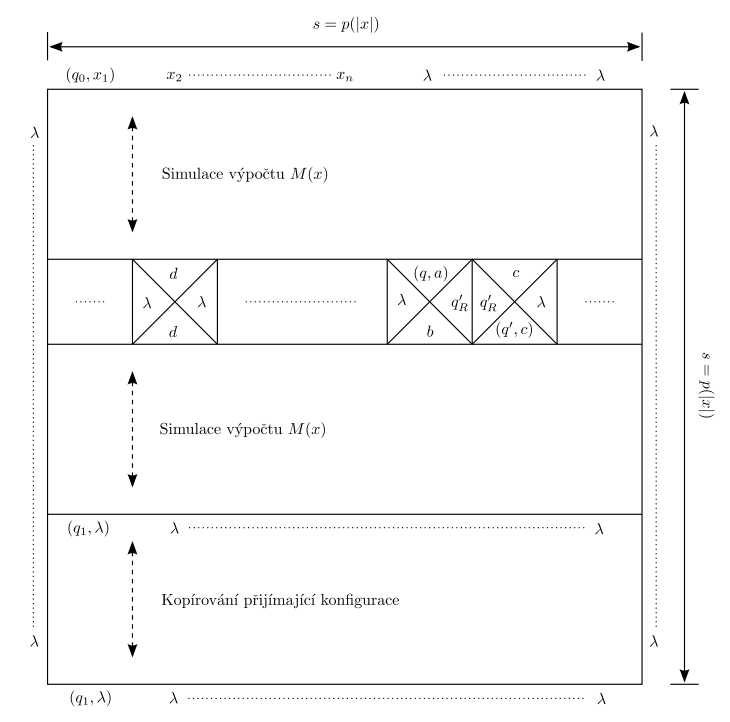
\includegraphics[width=0.8\textwidth]{img/kachl_overview.png}
\end{figure}

Barvy kachlíků tedy budou odpovídat symbolům, které potřebujeme pro zakódování konfigurace, ale budeme potřebovat i pomocné barvy pro přenos informace o stavu o kachlík vlevo nebo vpravo. Položíme tedy
$$ B = \Sigma \cup Q \times \Sigma \cup \{q_L, q_R\ |\ q \in Q\}$$

\begin{itemize}
	
	
	\item Barva $(q, a)$ v této konfiguraci bude kódovat políčko na pásce, nad kterým se vyskytuje hlava, přičemž $q$ označuje stav, ve kterém se $M$ nachází. Vždy je pouze jedna barva tohoto typu na řádku.
	\item Ostatní políčka konfigurace budou obarvena barvou odpovídající symbolu na daném místě.
	\item Velikost jedné strany čtvercové sítě položíme $s = p(|x|)$.
	\item Boční strany $S$ budou obarveny barvou $\lambda$ (prázdný symbol).
	\item Horní strana $S$ bude obarvena počáteční konfigurací: $[(q_0, x_1), x2, x3, \dots, x_n, \lambda, \dots,\lambda]$, pro vstup $x = x_1x_2x_3\dots x_n$.
	\item Spodní hrana $S$ bude obarvena jednoznačnou přijímající konfigurací: $[(q_1, \lambda), \lambda, \dots, \lambda]$
\end{itemize}

Do typů kachlíků zakódujeme přechodovou funkci Turingova stroje $M$, čímž dosáhneme toho, že správné vykachlíkování řádků 2 až $s$ bude odpovídat výpočtu $M$ nad $x$. Navíc přidáme možnost kopírování přijímající konfigurace tak, abychom ošetřili i případ, kdy výpočet $M$ nad $x$ skončí po méně než $p(|x|)$ krocích.

Použité kachlíky jsou vypsány v tabulce \ref{kachliky}.

\begin{table}[H]
	\centering
	\caption{Kachlíky}
	\label{kachliky}
	\renewcommand{\arraystretch}{1.5}
	\begin{tabular}{| m{0.05\linewidth}  m{0.45\linewidth} | m{0.5\linewidth}| }
		\hline
		(I) & \smallskip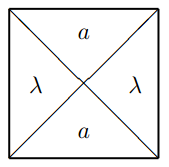
\includegraphics[width=70pt]{img/kachl1.png} 
		& $\forall a \in \Sigma$ kopírování buněk, nad nimiž není hlava\\ 
		(II) & 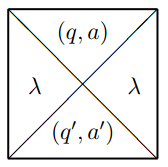
\includegraphics[width=70pt]{img/kachl2.png} 
		& $\forall q \forall a \forall q' \forall a' : (q',a',N) \in \delta(q,a)$\\ 
		(III), (IV) & 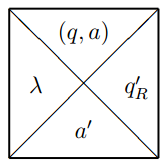
\includegraphics[width=70pt]{img/kachl3.png} 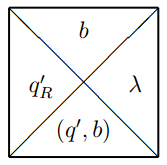
\includegraphics[width=70pt]{img/kachl4.png} 
		& $\forall q \forall a \forall q' \forall a' : (q',a',R) \in \delta(q,a)$\\
		(V), (VI) & 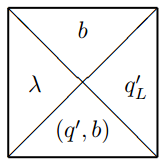
\includegraphics[width=70pt]{img/kachl5.png} 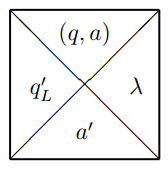
\includegraphics[width=70pt]{img/kachl6.png} 
		& $\forall q \forall a \forall q' \forall a' : (q',a',L) \in \delta(q,a)$\\
		(VII) & 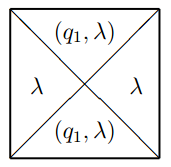
\includegraphics[width=70pt]{img/kachl7.png} 
		& \\ \hline

	\end{tabular}

\end{table}

Funkce f, která bude převádět instanci problému $A$ na instanci problému KACHL provede právě popsanou konstrukci, tj. z popisu $M$ a instance $x$ vytvoří instanci $(B, K, s, S)$, kde množina $K$ obsahuje popsané typy kachlíků a pod $S$ míníme obarvení okrajů sítě. Tuto konstrukci je zřejmě možné provést v polynomiálním čase. Jediné co je v konstrukci závislé na velikosti vstupu je tedy rozměr sítě $s = p(|x|)$ a obarvení horního okraje S počáteční konfigurací.

Zbývá ukázat, že $x \in A \Leftrightarrow $ takto zkonstruovaná instance KACHL má přípustné vykachlíkování:
\begin{description}
	
	\item[$\Rightarrow$:] 
	Předpokládejme nejprve, že $x \in A$ a tedy existuje přijímající výpočet $M(x)$ daný posloupností konfigurací $K_0^x = K_0, \dots, K_t = K_F$. Podle předpokladu platí, že $t \leq p(|x|)$ a délka slova na pásce v každé konfiguraci je rovněž nejvýš $p(|x|)$. Popíšeme, jak s pomocí konfigurací $K_0, \dots, K_t$ obarvit síť $S$. Pro řadu $i = 0$, tj. horní okraj $S$ je vybarvení správně díky konstrukci. Dále indukcí: máme-li validně vybarvenou $i$-tou řadu, vykachlíkujeme $(i + 1)$-ní řadu s odsimulováním příslušné instrukce, která vedla k přechodu z $K_i$ do $K_{i+1}$. Takto se dostaneme k $K_t = K_F$ a poté dokopírujeme KF až na poslední řádek čtvercové sítě $S$. 
	Instrukci lze vždy odsimulovat díky použitým typům kachlíků. 

	\item[$\Leftarrow$] Nechť $\exists$ přípustné vykachlíkování čtvercové sítě $S$. Ukážeme, že řádky barev mezi jednotlivými řádky kachlíků určují posloupnost konfigurací v přijímajícím výpočtu $M$ nad $x$. 
	
	Indukcí dle i: nechť $b_{i,1}, \dots, b_{i,s} \in B$ je posloupnost barev mezi $i$-tým a $(i+1)$-ním řádkem. Musíme ukázat tyto dvě vlastnosti pro každé $i = 0, \dots, s$:
	\begin{enumerate}
		
		
		\item V posloupnosti $b_{i,1}, \dots, b_{i,s}$ je \textbf{právě jedna barva} typu $(q, a) \in Q \times \Sigma$, ostatní jsou typu $a \in \Sigma$, tj. posloupnost $b_{i,1}, \dots, b_{i,s}$ \textbf{určuje validní konfiguraci} $K_i$.
		\item Platí, že $K_i$ lze z $K_{i-1}$ \textbf{vytvořit pomocí přechodové funkce} $\delta$ pro $i > 0$ a $K_0 = K_0^x$.
	\end{enumerate}

	Obě vlastnosti jsou jistě splněné pro $i = 0$. Předpokládejme nyní, že jsou splněny pro $i \in [0, \dots, s]$ a ukažme, že platí pro $i + 1$. Obě vlastnosti opět jednoduše plynou z toho, jaké kachlíky máme k dispozici. Podle indukčního předpokladu se na řádku barev vyskytuje právě jedna pozice, řekněme $k$, pro kterou platí, že $b_{i,k} = (q, a)$ pro nějaký stav $q \in Q$ a znak $a \in \Sigma$. To znamená, že v $(i + 1)$-ním řádku kachlíků je právě jeden kachlík s horní barvou $(q, a)$, a to na pozici $S[i+1, k]$. Kachlíky nám neumožňují vytvořit barvu $(q, a)$ z ničeho, musí jít o barvu tohoto typu převedenou z předchozího řádku, a to buď kachlíkem (II) a nebo kachlíky (III) a (IV) a nebo kachlíky (V) a (VI).

	Spodní hrana $S$ je obarvena přijímající konfigurací, takže poslední řada barev kachlíků musí
	odpovídat přijímající konfiguraci. 
	
	Dostáváme tedy, že posloupnost konfigurací daných barvami na hranách mezi řádky kachlíků v čtvercové síti $S$ odpovídají přijímajícímu výpočtu $M$ nad vstupem $x$ a jde dokonce o vzájemnou korespondenci, a tedy máme-li přípustné vykachlíkování, znamená to, že $M(x)$ přijme. Z toho plyne, že $x \in A.$
\end{description}


\end{proof}

\subsection{Další NP-úplné problémy}
\subsubsection{SAT -- Splnitelnost formule v KNF}
\begin{minipage}{\textwidth}
	\bigskip
	\centering
	\fbox{
		\parbox{0.7\textwidth}{
			\smallskip
			{\centering
				\textsc{Splnitelnost formule v KNF (SAT)}\\
			}
			\medskip		
			\textbf{Instance}: Formule $\varphi$ na $n$ proměnných v konjunktivně normální formě.
			\smallskip
			
			\textbf{Otázka:} Existuje ohodnocení proměnných $t \in \{0, 1\}^n$, pro které platí $\varphi(t) = 1$? Jinými slovy, existuje ohodnocení, pro které je $\varphi$ splněná?
		}
	}
	\bigskip
\end{minipage}

\begin{theorem}
SAT je NP-úplný.
\end{theorem}
\begin{proof}
\begin{enumerate}
	
	
	\item SAT $\in$ NP, ohodnocení $t$ umíme polynomiálně rychle ověřit.
	
	\item KACHL $\rightarrow$ SAT
	Sestrojíme $\varphi$ s $s^2 \cdot |K|$ proměnnými ($s^2$ velikost pole, $K$ počet typů kachlíků) tvaru $x_{i,j,k}, \text{ kde } i,j \in \{1\dots s\}, k \in \{1\dots|K|\} $ a hodnota $x_{i,j,k}$ vyjadřuje \uv{na poli $S[i,j]$ je kachlík typu $T_k$}.
	
	Definujeme:
	\begin{align*}
		V &= \{(p,q)\ |\ \text{spodní barva kachlíku typu $T_p$ se neshoduje s horní barvou $T_q$} \}\\
		H &= \{(p,q)\ |\ \text{prava barva kachlíku typu $T_p$ se neshoduje s levou barvou $T_q$} \}		
	\end{align*}
	a pro $i \in \{1, \dots s\}$ definujeme
	\begin{align*}
		U_i &= \{k |\ \text{horní barva $T_k$ se shoduje s barvou horního okraje S v $i$-tém sloupci} \}\\
		B_i &= \{k |\ \text{spodní barva $T_k$ se shoduje s barvou spodního okraje S v $i$-tém sloupci} \}\\
		L_i &= \{k |\ \text{levá barva $T_k$ se shoduje s barvou levé okraje S v $i$-tém řádku} \}\\
		R_i &= \{k |\ \text{pravá barva $T_k$ se shoduje s barvou pravého okraje S v $i$-tém řádku} \}\\
	\end{align*}

	Konstrukce $\varphi$:
	\begin{enumerate}
		
		\item $C_{i,j} = \bigvee\limits_{k=1}^{|K|} x_{i,j,k}$ \quad\dots\quad \uv{každé pole má kachlík}
		
		\item $\alpha_{i,j} = \bigwedge\limits_{k=1}^{|K|}\bigwedge\limits_{l=k+1}^{|K|} (\overline{x_{i,j,k}} \vee \overline{x_{i,j,l}})$ \quad\dots\quad \uv{každé pole má \textbf{nejvýše 1} kachlík}
		
		\item $\beta_{i,j} = C_{i,j} \wedge \alpha_{i,j}$ \quad\dots\quad \uv{každé pole má \textbf{právě 1} kachlík}
		
		\item $\gamma_{i,j} = \bigwedge\limits_{(p,q)\in V} (\overline{x_{i,j,p}} \vee \overline{x_{i+1,j,q}})$ \quad\dots\quad \uv{pole jsou \textbf{vertikálně} kompatibilní}
		
		\item $\delta_{i,j} = \bigwedge\limits_{(p,q)\in H} (\overline{x_{i,j,p}} \vee \overline{x_{i,j+1,q}})$ \quad\dots\quad \uv{pole jsou \textbf{horizontálně} kompatibilní}
		
		\item $\varepsilon = \bigwedge\limits_{j=1}^{s}\left(\bigvee\limits_{k\in U_j} x_{1,j,k} \right) \wedge \bigwedge\limits_{j=1}^{s}\left(\bigvee\limits_{k\in B_j} x_{s,j,k} \right) \wedge \bigwedge\limits_{j=1}^{s}\left(\bigvee\limits_{k\in L_j} x_{j,1,k} \right) \wedge \bigwedge\limits_{j=1}^{s}\left(\bigvee\limits_{k\in R_j} x_{j,s,k} \right)$ 
		\medskip
		
		\quad\dots\quad \uv{okraje jsou kompatibilní}
	\end{enumerate}

	Nyní
	$$\varphi = \bigwedge\limits_{i=1}^{s}\bigwedge\limits_{j=1}^{s} \beta_{i,j} \wedge \bigwedge\limits_{i=1}^{s-1}\bigwedge\limits_{j=1}^{s} \gamma_{i,j} \wedge \bigwedge\limits_{i=1}^{s}\bigwedge\limits_{j=1}^{s-1}\delta_{i,j} \wedge \varepsilon$$
\end{enumerate}

\textbf{Ekvivalence:} pokud existuje vykachlíkování, tak existuje splňující ohodnocení $\varphi$: $x_{i,j,k} = 1$ pokud na $S[i,j]$ je kachlík typu $T_k$; 0 jinak. Pokud existuje ohodnocení, tak vykachlíkujeme takto: díky $\beta$ existuje pro $\forall i,j$ právě 1 $k$ takové, že $x_{i,j,k} = 1 \rightarrow$ na $S[i,j]$ umístíme $T_k$.
\end{proof}

\subsubsection{3SAT -- Splnitelnost formule ve 3KNF}
\begin{minipage}{\textwidth}
	\bigskip
	\centering
	\fbox{
		\parbox{0.7\textwidth}{
			\smallskip
			{\centering
				\textsc{Splnitelnost formule v 3KNF (3SAT)}\\
			}
			\medskip		
			\textbf{Instance}: Formule $\varphi$ na $n$ proměnných v 3KNF (každá klauzule obsahuje \textbf{právě 3} literály).
			\smallskip
			
			\textbf{Otázka:} Existuje ohodnocení proměnných $t \in \{0, 1\}^n$, pro které platí $\varphi(t) = 1$? Jinými slovy, existuje ohodnocení, pro které je $\varphi$ splněná?
		}
	}
	\bigskip
\end{minipage}

\begin{theorem}
	3SAT je NP-úplný.
\end{theorem}
\begin{proof}(idea)
	\begin{enumerate}

	
	
	\item 3SAT $\in$ NP, ohodnocení $t$ umíme polynomiálně rychle ověřit.
	
	\item SAT $\rightarrow$ 3SAT
	Z formule $\psi = C_1 \wedge C2 \wedge \dots \wedge C_m$ v KNF sestrojíme $\varphi$ v 3KNF.
	
	$\forall C_i = (e_1 \vee e_2 \vee \dots \vee e_k) \rightarrow \alpha_i$
	\begin{itemize}
		
		
		\item $k = 1$: \quad $\alpha_i = (e_1 \vee y_1^j \vee y_2^j) \wedge (e_1 \vee y_1^j \vee \overline{y}_2^j) \vee (e_1 \vee \overline{y}_1^j \vee y_2^j) \vee (e_1 \vee \overline{y}_1^j \vee \overline{y}_2^j)$
		
		\item $k = 2$: \quad $\alpha_i = (e_1 \vee e_2 \vee y^j) \wedge (e_1 \vee e_2 \vee \overline{y}^j)$
		
		\item $k = 2$: \quad $\alpha_i = C_i$
		
		\item $k > 3$: \quad $\alpha_i = (e_1 \vee e_2 \vee y_1^j) \wedge (\overline{y}_1^j \vee e_3 \vee e_2 \vee y_2^j) \wedge \dots \wedge (\overline{y}_{k-3}^j \vee e_{k-1} e_k)$
	\end{itemize}
	Kde všechna $y$ jsou nové proměnné. Pak $\varphi = \bigwedge\limits_{j=1}^m$. Konstrukce je polynomiální. Ekvivalence rozborem případů.
	\end{enumerate}
\end{proof}


\subsubsection{VP -- Vrcholové pokrytí}
\begin{minipage}{\textwidth}
	\bigskip
	\centering
	\fbox{
		\parbox{0.7\textwidth}{
			\smallskip
			{\centering
				\textsc{Vrcholové pokrytí (VP) (angl. vertex cover)}\\
			}
			\medskip		
			\textbf{Instance}: Graf $G = (V,E)$ a přirozené číslo $k$.
			\smallskip
			
			\textbf{Otázka:} Existuje množina $S \subseteq V$ , která obsahuje nejvýš $k$ vrcholů a z každé hrany obsahuje alespoň jeden koncový vrchol? (Tj. $|S| \leq k$ a $(\forall e \in E)[S \cap e \neq \emptyset]$.)
		}
	}
	\bigskip
\end{minipage}

\begin{theorem}
VP je NP-úplný.
\end{theorem}
\begin{proof}(idea)
Převodem 3SAT $\rightarrow$ VP. Příklad:
\begin{figure}[H]
	\centering
	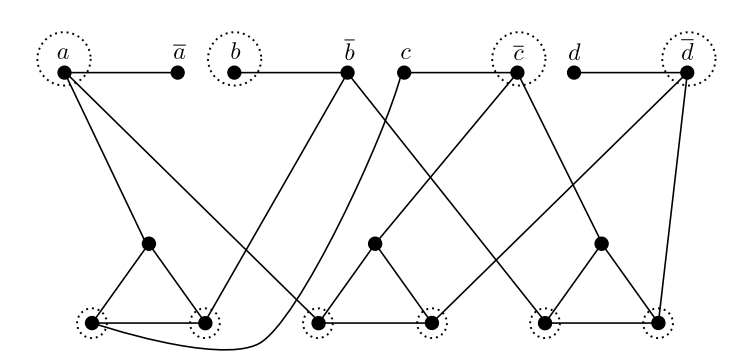
\includegraphics[width=0.7\textwidth]{img/vertexcover.png}
	\caption{Příklad převodu formule $\varphi = (a \vee b \vee c)\wedge(a \vee c \vee d)\wedge(b \vee c \vee d)$ na instanci VP. Jednotlivé trojúhelníky dole odpovídají klauzulím, zakroužkované vrcholy určují vrcholové pokrytí velikosti k, které odpovídá splňujícímu ohodnocení a = b = 1, c = d = 0.}
\end{figure}

\end{proof}


\subsubsection{HK -- Hamiltonovská kružnice}
\begin{minipage}{\textwidth}
	\bigskip
	\centering
	\fbox{
		\parbox{0.7\textwidth}{
			\smallskip
			{\centering
				\textsc{Hamiltonovská kružnice (HK)}\\
			}
			\medskip		
			\textbf{Instance}: Graf $G = (V,E)$.
			\smallskip
			
			\textbf{Otázka:} Existuje v $G$ cyklus vedoucí přes všechny vrcholy?
		}
	}
	\bigskip
\end{minipage}

\begin{theorem}
	HK je NP-úplný.
\end{theorem}
\begin{proof}(idea)
Převodem z VP. Pro graf $G = (V,E)$ chceme najít VP velikosti $k$, zkonstruujeme $G' = (V', E')$ tak, že:
\begin{itemize}
	\item pro každou hranu $(u,v) \in E$ vytvoříme podgraf jako na obrázku \ref{ham1}(a).
	\begin{figure}[H]
		\centering
		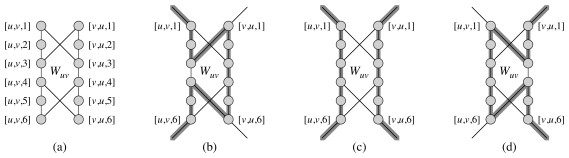
\includegraphics[width=0.7\textwidth]{img/hamilton1.jpg}
		\label{ham1}
		\caption{Podgraf pro hranu (u,v)}
	\end{figure}
	Hamiltonovská kružnice může projít tímto podgrafem pouze 3 způsoby naznačenými na obrázku \ref{ham1}(b,c,d): 
	\begin{enumerate}
		
		
		\item (b) hrana je pokrytá vrcholem $u$
		\item (c) hrana je pokrytá oběma vrcholy $u, v$
		\item (d) hrana je pokrytá vrcholem $v$
	\end{enumerate}

	\item do $V'$ přidáme $k$ \uv{výberových} vrcholů $s_1, \dots s_k$
	
	\item pro každý vrchol $v$ spojíme všechny podgrafy odpovídající jemu incidentním hranám do řetízku pod sebe (tj. $(v,x,6)$ napojíme na $(v,y,1)$ atd.). Konce tohoto řetízku spojíme hranou se všemi výběrovými vrcholy $s_1, \dots, s_k$
	
	\begin{figure}[H]
		\centering
		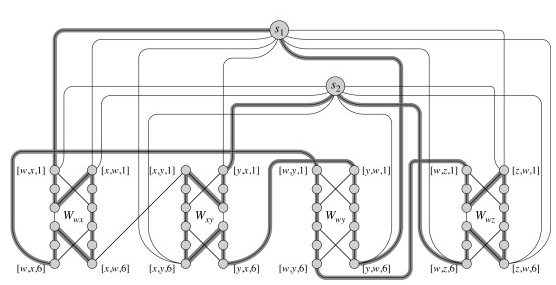
\includegraphics[width=0.9\textwidth]{img/hamilton2.jpg}
		\label{ham2}
		\caption{Výsledné zapojení.}
	\end{figure}
\end{itemize}
\end{proof}


\subsubsection{3DM -- Trojrozměrné párování}
\begin{minipage}{\textwidth}
	\bigskip
	\centering
	\fbox{
		\parbox{0.7\textwidth}{
			\smallskip
			{\centering
				\textsc{Trojrozměrné párování (3DM)}\\
			}
			\medskip		
			\textbf{Instance}: Množina $M \subseteq W \times X \times Y$, kde $W, X, Y$ jsou po dvou disjunktní
			množiny, z nichž každá obsahuje právě $q$ prvků.
			\smallskip
			
			\textbf{Otázka:} Obsahuje $M$ perfektní párování? Jinými slovy, existuje množina $M' \subseteq M, |M'| = q$, trojice v níž obsažené jsou po dvou disjunktní?
		}
	}
	\bigskip
\end{minipage}

Převodem ze SAT.

\subsubsection{LOUP -- Loupežníci}
\begin{minipage}{\textwidth}
	\bigskip
	\centering
	\fbox{
		\parbox{0.7\textwidth}{
			\smallskip
			{\centering
				\textsc{Loupežníci (LOUP)} (angl. Partition)\\
			}
			\medskip		
			\textbf{Instance}: Množina prvků $A$ a s každým prvkem $a \in A$ asociovaná cena (váha, velikost,\dots) $s(a) \in \N$.
			\smallskip
			
			\textbf{Otázka:} Lze rozdělit prvky z $A$ na dvě poloviny s toutéž celkovou cenou? Přesněji, existuje množina $A' \subseteq A$ taková, že
			$$\sum\limits_{a \in A'} s(a) = \sum\limits_{a \in A \setminus A'} s(a)\ ?$$
		}
	}
	\bigskip
\end{minipage}

Převodem ze 3DM.

\subsubsection{Další}
\begin{itemize}
\item \textbf{Klika:} Převodem z VP: Má $G=(V,E)$ VP velikosti $k$? $\to$ Má $\overline{G}(V,\overline{E})$ kliku velikosti $|V| - k$?
\begin{figure}[H]
	\centering
	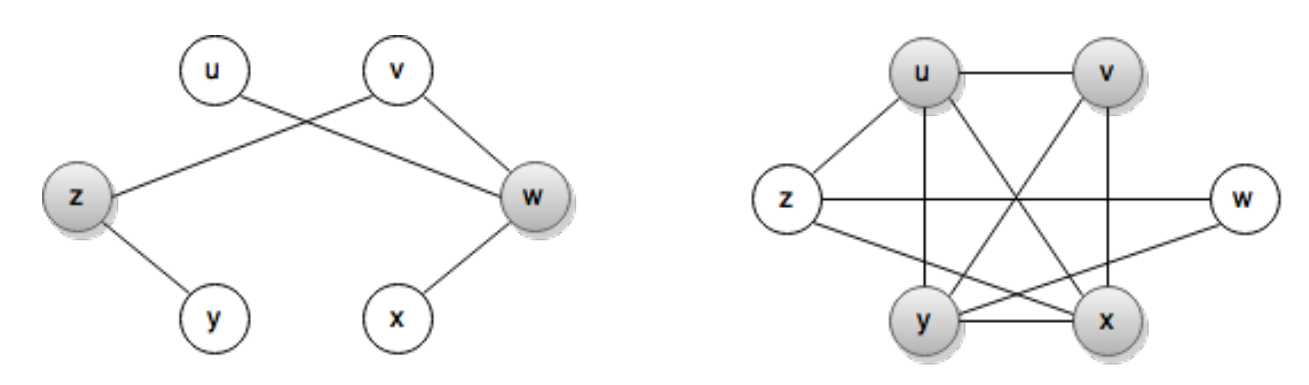
\includegraphics[]{img/vertex_clique.png}
\end{figure}

\item \textbf{Nezávislá množina:} Duální problém ke Klice.
\item \textbf{Orientovaná HK:} Triviálně převodem z HK: Neorientovaný graf převedeme na orientovaný zdvojením hran.
\item \textbf{Hamiltonovská cesta z $s$ do $t$:} Triviálně převodem z HK: Existuje v $G$ HK $\to$ Existuje v $G$ HC z $v_0$ do $v_0$ pro libovolný vrchol $v_0 \in V$.
\item \textbf{Hamiltonovská cesta:} Převodem z HK: zvolíme libovolný vrchol $v_0$, přidáme do grafu vrcholu $u, u', w$ a hrany $(u,u'), (w,v_0)$ a $(u,v)$ pro každý vrchol $v$ sousedící s $v_0$. Každá HC musí začínat hranou $(u,u')$ a končit hranou $(w,v_0)$.
\begin{figure}[H]
	\centering
	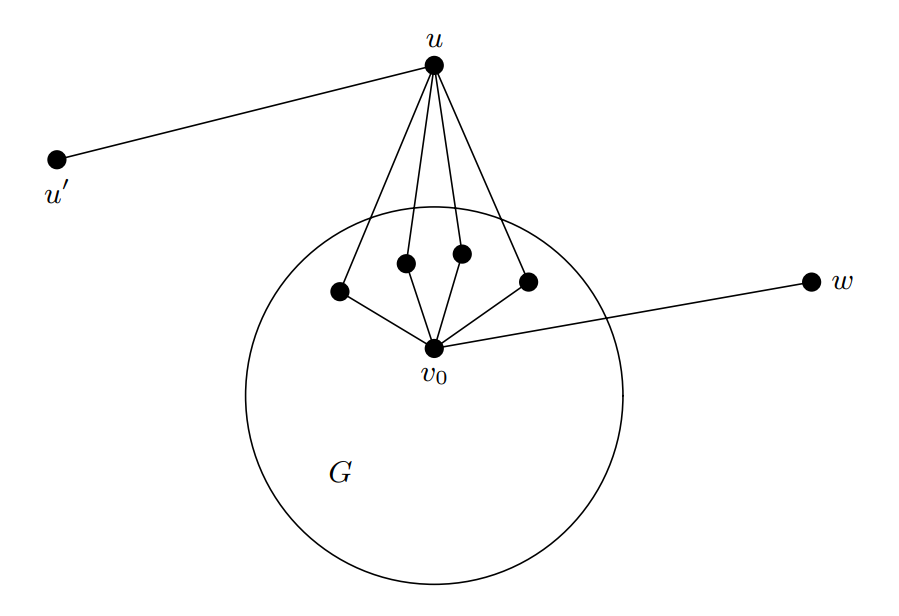
\includegraphics[]{img/hkhc.png}
\end{figure}

\item \textbf{Obchodní cestující:} Převodem z HC: Původní $G$ doplníme na kompletní graf $G'$, nově přidané hrany mají cenu 1, původní hrany mají cenu 0. Existuje HC $\to$ existuje řešení TSP s cenou 0?
\item \textbf{Batoh:} Převodem z Loupežníků. Nastavíme $c(a) = v(a) = s(a)$, $B = \sum_{a\in A} s(a)/2$.
\item \textbf{Rozvrhování:} Převodem z Batohu nebo Loupežníků.
\item \textbf{Dominující množina:} Graf $G=(V,E)$, existuje $S \subseteq V, |S| \leq k$ taková, že každý vrchol z $V$ buď je v $S$ nebo má v $S$ souseda.

Převodem z VP: pro každou hranu $(u,v)$ přidáme vrchol $w_{u,v}$, ten spojíme hranou s $u$ i s $v$ (kdyby byl vybrán do dominující množiny, lze jej bez zhoršení výsledku nahradit $u$ nebo $v$).
\item \textbf{Hitting set:} Množina $S$ a množina $C$ podmnožin množiny $S$. Existuje $S'\subseteq S, |S'| \leq k$ taková, že $S'$ obsahuje nejméně jeden prvek z každé množiny v $C$?

Převod z VP: $S = V, C = \{\{u,v\}\ |\ (u,v)\in E\}$. 
\item \textbf{Čtyřlistá kostra:} Převodem z HC(s,t). Vrcholům $s$ a $t$ přidáme \uv{uši}.
\item \textbf{Největší společný podgraf:} Převodem z Kliky: Graf $G$ má kliku velikosti $k$ $\to$ $G$ a $K_k$ mají společný graf velikosti $k$.
\item \textbf{Množinové pokrytí:} Máme $S = S_1, S_2, \dots S_n$ podmnožiny $U$, existuje podmnožina $S$ taková, že sjednocení $S_i$ v této podmnožine je $U$? 

Převod z VP: Má $G=(V,E)$ VP velikosti $k$? $\to$ Má $U = E, \forall i \in V : S_i = \{\text{hrany incidentní $i$}\}$  množinové pokrytí velikosti $k$?
\end{itemize}


\section{Pseudopolynomiální algoritmy, silná NP-úplnost.}
I mezi různými NP-úplnými problémy a úlohami může být co do složitosti jejich řešitelnosti rozdíl. 

\subsection{Pseudopolynomiální algoritmy}
Nechť $A$ je libovolný rozhodovací problém a $I$ nechť je instance tohoto problému. Potom 
\begin{description}
	
	
	\item[$len(I)$] označuje \textbf{délku zakódování} instance $I$ při standardním \textit{binárním} kódování.
	\item[$max(I)$] označuje hodnotu \textbf{největšího číselného parametru}, který se vyskytuje v $I$.
\end{description}
Řekneme, že $A$ je \textbf{číselný problém}, pokud pro každý polynom $p$ existuje instance $I$ tohoto problému taková, že
$max(I) > p(len(I))$. \textit{Intuitivně: pokud je v problému nějaký parametr, kterého fakt záleží, jestli je to 10 nebo 1000000000 a ovlivní to rychlost běhu algoritmu, pak je to číselný problém.}

Například \textsc{Batoh} nebo \textsc{Loupežníci} jsou číselné problémy. \textsc{Splnitelnost} nebo \textsc{Kachlíkování} číselné nejsou.

Řekneme, že algoritmus, který řeší problém $A$, je \textbf{pseudopolynomiální}, pokud je jeho časová složitost omezena
polynomem dvou proměnných \textit{len(I)} a \textit{max(I)}. \textit{Intuitivně: algoritmus je v podstatě polynomiální, ale visí na tom nějakém parametru, který může být třeba i 100000000000. }

Druhý pohled na věc je, že pseudopolynomiální algoritmus by byl polynomiální, pokud předáme vstup zakódovaný \textbf{unárně}. \textit{Intuitivně: pak totiž musíme těch 1000000000000 kódovat jako 1000000000000 jedniček, takže pak velikost vstupu reflektuje ten astronomicky velký parametr.}

Je-li problém A řešitelný pseudopolynomiálním algoritmem a není-li A číselný problém, pak je zřejmě tento pseudopolynomiální algoritmus ve skutečnosti polynomiální. 

\subsubsection{Příklad: Batoh}
\begin{minipage}{\textwidth}
	\bigskip
	\centering
	\fbox{
		\parbox{0.7\textwidth}{
			\smallskip
			{\centering
				\textsc{Batoh (Knapsack)}\\
			}
			\medskip		
			
			\textbf{Instance}: Množina n předmětů $A = \{a_1, \dots, a_n\}$, s každým předmětem asociovaná velikost $s(a_i) \in \N$ a cena či hodnota $v(a_i) \in \N$.
			Přirozené číslo $B \geq 0$ udávající velikost batohu.
			\medskip
			
			\textbf{Cíl}: Nalézt množinu předmětů $A' \subseteq A$, která dosahuje maximální
			souhrnné hodnoty předmětů v ní obsažených, a přitom se předměty z $A'$ vejdou do batohu velikosti $B$. Tj. chceme, aby platilo:
			$$\sum\limits_{a \in A'} s(a) \leq B$$
			$$\sum\limits_{a\in A'} v(a) = \max_{A'' \subseteq A,\ \sum_{a \in A'} s(a) \leq B} \sum\limits_{a \in A''} v(a)$$
		}
	}
	\bigskip
\end{minipage}


Následující pseudopolynomiální algoritmus je založen na dynamickém programování. Na vstupu očekává jen předměty, které se do batohu vejdou a současně jejich velikost je nenulová ($\forall i \in \{1, \dots, n\} : 0 < s[i] \leq B$).
\bigskip

\begin{minipage}{\linewidth}
	\label{batoh_pp}
	\begin{lstlisting}[language=Python, frame=single, escapeinside={\%*}{*)}]
Batoh(s, v, B): 
	# s ... pole velikosti predmetu
	# v ... pole cen predmetu
	# B ... velikost batohu
	V = sum(v[i] for i in range(1,n))
	n = len(s)
	T = [,]
	S = [,]
	for c in range (1, V):
		T[0, c] = None
		S[0, c] = B + 1
	for j in range(0, n):
		T[j,0] = None
		S[j,0] = 0
		for c in range(1, V):
			T[j, c] = T[j - 1, c]
			S[j, c] = S[j - 1, c]
			if v[j] <= c and S[j, c] > S[j - 1, c - v[j]] + s[j]:
				T[j, c] = union(T[j - 1, c - v[j]], {j})
				S[j, c] = S[j - 1, c - v[j]] + s[j]
	cc = max{c for (n,c) in S if S[n, c] <= B}
	return T[n, cc]
		
	\end{lstlisting}
\end{minipage}
\bigskip

$T$ je tabulka typu $(n + 1) \times (V + 1)$, na pozici $T[j, c], 0 \leq j \leq n, 0 \leq c \leq V$ , bude podmnožina indexů $\{1, \dots, j\}$ prvků celkové ceny přesně $c$ s minimální velikostí.

$S$ je tabulka typu $(n+1)\times(V +1)$, na pozici $S[j, c]$ je celková velikost předmětů
v množině $T[j, c]$. Pokud neexistuje množina s předměty ceny přesně $c$, je na pozici
$S[j, c]$ číslo $B + 1$.

Popsaný algoritmus pracuje v čase $\Theta(nV)$ (počítáme-li aritmetické operace jako konstantní). Zdá se, tedy, že jde o polynomiální algoritmus, ale musíme si uvědomit, že velikost vstupu je při standardním binárním kódování pouze $O(n \log_2(B + V ))$ a $V$ tedy může být \textit{exponenciálně} větší než vstup ($\Rightarrow$ je to číselný problém). Formálně tedy $len(I) = O(n\log_2(B+V))$, zatímco $max(I) = max(\{B\} \cup \{v[i], s[i]\ |\ 1 \leq i \leq n \})$ a dle definice jde tedy skutečně o pseudopolynomiální algoritmus.


\subsection{Silná NP-úplnost}
Nechť $A$ je NP-úplný problém a $p$ je polynom. Pomocí $A(p)$ označíme restrikci problému $A$ na instance $I$, pro něž
platí $max(I) \leq p(len(I))$.

Řekneme, že problém $A$ je \textbf{silně NP-úplný}, pokud existuje polynom $p$, pro který $A(p)$ je NP-úplný problém.
\textit{Intuitivně: omezení $A(p)$ nám dá pouze \uv{nečíselné instance}, tj. takové, kde jsou číselné parametry rozumně malé (jdou omezit polynomem). Pokud i tyhle \uv{rozumné} instance jsou NP-úplné, tak je to fakt silně NP-úplný problém}

Řekneme, že problém $A$ je \textbf{slabě NP-úplný}, pokud pro něj existuje pseudopolynomiální algoritmus.

\textit{Pozn.: Jsou NP-úplné problémy, které nejsou ani silně, ani slabě NP-úplné.}

\textbf{Každý nečíselný NP-úplný problém je silně NP-úplný.} Neboť pro nečíselný problém existuje polynom $p$ takový, že pro \textit{každou} instanci $I$ platí $max(I) \leq p(len(I))$, a pak tedy $A(p) = A$, který je NP-úplný (tj. restrikce podle tohoto polynomu $p$ zachová \textit{všechny} instance původního problému)).

Pokud by existoval silně NP-úplný problém, který lze vyřešit pseudopolynomiálním algoritmem, znamenalo by
to, že P = NP.

Silně NP-úplný problém je NP-úplný i při unárním kódování.

I číselné NP-úplné problémy mohou být silně NP-úplné, například \textsc{Rozvrhování} nebo \textsc{Bin Packing}. Ukážeme že to platí i pro \textsc{TSP}:

\begin{minipage}{\textwidth}
	\bigskip
	\centering
	\fbox{
		\parbox{0.7\textwidth}{
			\smallskip
			{\centering
				\textsc{Travelling Salesman Problem (TSP) - rozhodovací verze}\\
			}
			\medskip		
			
			\textbf{Instance}: Množina měst $C = \{c_1, \dots, c_n\}$, hodnoty $d(c_i, c_j) \in \N$ přiřazující každé dvojici měst vzdálenost a $D \in \N$.
			\medskip
			
			\textbf{Otázka}: Existuje permutace měst $c_{\pi(1)}, c_{\pi(2)}, \dots, c_{\pi(n)}$, pro kterou platí, že
			
			$$\left(\sum\limits_{i=1}^{n-1} d(c_{\pi(i)}, c_{\pi(i+1)}) \right) + d(c_{\pi(n)}, c_{\pi(1)}) \leq D\quad ?$$
		}
	}
	\bigskip
\end{minipage}

\begin{theorem}
	Problém obchodního cestujícího (rozhodovací verze) je silně NP-úplný.
\end{theorem}
\begin{proof}
Problém TSP jistě patří do třídy NP, neboť jsme schopni ověřit v polynomiálním čase, zda daná permutace měst splňuje naše požadavky, a zřejmě i $TSP(p)$ patří do NP pro každý polynom $p$. Těžkost problému $TSP(p)$ pro vhodně zvolený polynom $p$ si ukážeme převodem z problému \textit{Hamiltonovské kružnice v neorientovaném grafu}. 

Uvažme neorientovaný graf $G = (V, E)$ a sestavme na jeho základě instanci obchodního cestujícího následujícím způsobem:
\begin{itemize}
	
	
	\item Množinu měst $C$ položíme rovnu množině vrcholů $V$, tedy $C = V = \{v_1, \dots, v_n\}$.
	\item Vzdálenost mezi městy či vrcholy $v_i$ a $v_j$ pro $i \neq j$ a $i, j \in \{1, \dots, n\}$ určíme následujícím
	předpisem:
	$$
	d(vi, vj) = 
	\begin{cases}
	0 & \quad \text{pokud } \{v_i, v_j\} \in E \\
	1 & \quad \text{jinak} \\
	\end{cases}
	$$
	\item Hodnotu D položíme rovnu 0. 
\end{itemize}

Není těžké ukázat, že v grafu G existuje hamiltonovská kružnice, právě když v sestrojené instanci obchodního cestujícího existuje cyklus nulové délky, který obejde všechna města, přičemž navštíví každé z nich právě jednou. Z jedné strany hamiltonovská kružnice využívá jen hrany nulové délky, z druhé strany cesta nulové délky využívá jen hrany grafu G. Hodnota maximálního číselného parametru v sestrojené instanci je přitom rovna 1, tedy omezená verze problému $TSP(1)$ je stále NP-úplná, což znamená, že problém TSP je silně NP-úplný.	
\end{proof}



\section{Aproximační algoritmy a schémata.}
Pokud nejsme schopni rychle získat optimální řešení NP-úplné úlohy, můžeme slevit ze svých požadavků a pokusit se najít řešení, jež není od toho optimálního příliš vzdáleno. Nejprve si upřesníme pojem optimalizační úlohy:

\subsection{Optimalizační úloha}
\textbf{Optimalizační úlohu} definujeme jako trojici $A = (D_A, S_A, \mu_A)$, kde
\begin{itemize}
	
	
	\item $D_A \subseteq \Sigma^*$ je \textbf{množina instancí}
	\item $S_A(I)$ je \textbf{množina přípustných řešení} pro instanci $I \in D_A$
	\item $\mu_A(I, \sigma)$ přiřazuje instanci $I \in D_A$ a přípustnému řešení  $\sigma \in S_A(I)$ kladné racionální číslo, tzv. \textbf{hodnotu řešení}.
\end{itemize}

Úloha může být $A$ \textbf{maximalizační} resp. \textbf{minimalizační}, pak optimálním řešením instance $I$ je to přípustné řešení $\sigma \in S_A(I)$, jež má \textit{maximální} resp. \textit{minimální} hodnotu $\mu_A(I, \sigma)$.

\textbf{Hodnotu optimálního řešení} označíme pomocí $opt(I)$.

Příklad: Minimalizační úloha \textit{Vrcholového pokrytí (VP)}: 
\begin{itemize}
	
	
	\item množina instancí $D_{VP}$ = všechny řetězce kódující nějaký graf $G = (V,E)$	
	\item množina přípustných řešení pro instanci $G$, tj. $S_{VP}(G)$ = všechny množiny vrcholů $S \subseteq V$ pokrývající všechny hrany
	\item hodnota řešení S, tj. $\mu_{VP}(G,S) = |S|$, tedy počet vrcholů v množině
\end{itemize}

\subsection{Aproximační algoritmus}
Algoritmus $R$ nazveme \textbf{aproximačním algoritmem} pro optimalizační úlohu $A$, pokud pro každou instanci $I \in D_A$ je výstupem $R(I)$ přípustné řešení $\sigma \in S_A(I)$ (pokud nějaké existuje). Označení $R(I)$ budeme často používat přímo pro hodnotu řešení $\sigma$ vráceného algoritmem $R$ na instanci $I$, tj. $R(I) = \mu_A(I, \sigma)$.

Je-li $A$ \textit{maximalizační} úloha, pak $\varepsilon \geq 1$ je \textbf{aproximačním poměrem} algoritmu $R$, pokud pro každou instanci $I \in D_A$ platí, že 
$$opt(I) \leq \varepsilon \cdot R(I)$$

Je-li $A$ \textit{minimalizační} úloha, pak $\varepsilon \geq 1$ je \textbf{aproximačním poměrem} algoritmu $R$, pokud pro každou instanci $I \in D_A$ platí, že 
$$R(I) \leq \varepsilon \cdot opt(I)$$

\subsubsection{Příklad: Bin Packing}
\begin{minipage}{\textwidth}
	\bigskip
	\centering
	\fbox{
		\parbox{0.7\textwidth}{
			\smallskip
			{\centering
				\textsc{Bin Packing (BP)}\\
			}
			\medskip		
			
			\textbf{Instance}: Konečná množina předmětů $U = \{u_1, \dots, u_n\}$, s každým předmětem asociovaná velikost $s(u)$, což je racionální číslo, pro které platí $0 \leq s(u) \leq 1$.
			\medskip
			
			\textbf{Cíl}: Najít rozdělení všech předmětů do co nejmenšího počtu po dvou disjunktních množin $U_1, . . . , U_m$ takové, že 
			$$(\forall i \in \{1, \dots, m\}) \left( \sum\limits_{u\in U_i} s(u) \leq 1\right)$$
			
			Naším cílem je minimalizovat $m$.
		}
	}
	\bigskip
\end{minipage}

Rozhodovací varianta je ekvivalentní problému \textsc{Rozvrhování}, a tedy i úloha \textsc{Bin Packing} je NP-těžká. Zkusíme navrhnou aproximační algoritmus:

\medskip
\noindent\textbf{Algoritmus 1: First Fit (FF)}: 
\begin{enumerate}
	
	
	\item Ber jeden předmět po druhém, pro každý předmět u najdi první koš, do nějž se tento předmět ještě vejde.
	\item Pokud takový koš neexistuje, přidej nový koš obsahující jen předmět $u$.  
\end{enumerate}

\begin{theorem}
	Pro každou instanci $I \in D_{BP}$ platí, že $FF(I) < 2 \cdot opt(I)$.
\end{theorem}
\begin{proof}

V řešení, které vrátí FF, je nejvýš jeden koš, který je zaplněn nejvýš z poloviny. Kdyby totiž existovaly dva koše $U_i, U_j$ pro $i \neq j$, které jsou zaplněny nejvýš z poloviny, tak by FF nepotřeboval zakládat nový koš pro předměty z $U_j$, všechny by se vešly do $U_i$. Pokud $FF(I) > 1$, pak z toho plyne, že
	$$FF(I) < \lceil 2\sum\limits_{i=1}^{n} s(u_i)\rceil \leq 2 \lceil \sum\limits_{i=1}^{n}s(u_i)\rceil$$
kde první nerovnost plyne z toho, že po zdvojnásobení obsahu jsou všechny koše plné až na jeden, který může být zaplněn jen částečně. Rovnosti bychom přitom dosáhli jedině ve chvíli, kdy by byly všechny koše zaplněné právě z poloviny, což není podle našeho předpokladu možné. Druhá nerovnost plyne z vlastností zaokrouhlování.

Na druhou stranu musí platit, že
	$$opt(I) \geq \lceil \sum\limits_{i=1}^{n} s(u_i)\rceil$$
Dohromady tedy dostaneme, že $FF(I) < 2 \cdot opt(I)$. Pokud $FF(I) = 1$, pak i $opt(I) = 1$ a i v tomto případě platí ostrá nerovnost.
\end{proof}

\begin{theorem}
Pro libovolné $k$ existuje instance $I \in D_{BP}$, pro niž je $opt(I) \geq k$ a FF vytvoří pro I aspoň $\frac{5}{3}opt(I)$ košů.
\end{theorem}
\begin{proof}
	Instance bude mít $U = \{u_1, u_2, \dots, u_{18k}\}$, s těmito prvky asociujeme váhy takto:
	$$
	s(u_i) =
	\begin{dcases}
	\frac{1}{7} + \varepsilon &\quad 1 \leq i \leq 6k\\
	\frac{1}{3} + \varepsilon &\quad 6k < i \leq 12k	\\
	\frac{1}{2} + \varepsilon &\quad 12k < i \leq 18k \\
	\end{dcases}
	$$
	kde $\varepsilon > 0$ je dostatečně malé kladné racionální číslo takové, že 
	$\left(\frac{1}{7} + \varepsilon + \frac{1}{3} + \varepsilon + \frac{1}{2} + \varepsilon\right) \leq 1$ a zároveň $6\cdot\left( \frac{1}{7} + \varepsilon \right) \leq 1$ a zároveň
	$2\cdot\left(\frac{1}{3} + \varepsilon\right) \leq 1$ a zároveň
	$\left(\frac{1}{2} + \varepsilon\right) \leq 1$.

	Optimální rozdělení rozdělí prvky do $6k$ košů. Algoritmus FF bude brát prvky jeden po druhém a vytvoří nejprve $k$ košů, každý s 6 prvky velikosti $\frac{1}{7} + \varepsilon$, poté $3k$ košů, každý se 2 prvky velikosti $\frac{1}{3} + \varepsilon$ a nakonec $6k$ košů, každý s jedním prvkem velikosti $\frac{1}{2} + \varepsilon$. Dohromady je tedy $10k$ košů, a tedy 
	$$\frac{FF(I)}{opt(I)} = \frac{5}{3}$$
\end{proof}

\medskip
\noindent\textbf{Algoritmus 2: First Fit Decreasing (FFD)}: 
\begin{enumerate}
	
	
	\item \textbf{Setřiď předměty sestupně podle velikosti.} 
	\item Ber jeden předmět po druhém \textbf{(od největšího po nejmenší)}, pro každý předmět $u$ najdi první koš, do nějž se tento předmět ještě vejde.
	\item Pokud takový koš neexistuje, přidej nový koš obsahující jen předmět $u$.  
\end{enumerate}

\begin{theorem}[BD]
	Pro každou instanci $I \in D_{BP}$ platí, že $FFD(I) < \frac{11}{9} \cdot opt(I) + 4$.
\end{theorem}
\begin{theorem}
	Pro libovolné $k$ existuje instance $I \in D_{BP}$, pro niž je $opt(I) \geq k$ a FF vytvoří pro I aspoň $\frac{11}{9}opt(I)$ košů.
\end{theorem}
\begin{proof}
	Instance bude mít $U = \{u_1, u_2, \dots, u_{30k}\}$, s těmito prvky asociujeme váhy takto:
	$$
	s(u_i) =
	\begin{dcases}
	\frac{1}{2} + \varepsilon 	&\quad 1 \leq i \leq 6k\\
	\frac{1}{4} + 2\varepsilon 	&\quad 6k < i \leq 12k	\\
	\frac{1}{4} + \varepsilon 	&\quad 12k < i \leq 18k \\
	\frac{1}{4} - 2\varepsilon 	&\quad 18k < i \leq 30k \\
	\end{dcases}
	$$
	kde $\varepsilon > 0$ je dostatečně malé kladné racionální číslo (prostě aby to všechno zase vyšlo).
	
	Optimální rozdělení rozdělí prvky do $9k$ košů (zcela zaplněných). Algoritmus FFD vytvoří $11m$ košů.
\end{proof}


\subsection{Aproximační schémata}
Lze dosáhnout \uv{libovolně malého} aproximačního poměru? Co kdybychom si mohli aproximační poměr předepsat?

Algoritmus ALG je \textbf{aproximačním schématem} pro optimalizační úlohu \textit{A}, pokud na vstupu očekává instanci
$I \in D_A$ a racionální číslo $\varepsilon > 0$ a na výstupu vydá řešení $\sigma \in S_A(I)$ s aproximačním poměrem $(1 + \varepsilon)$. Tj. pro maximalizační úlohu platí, že 
$$opt(I) \leq (1 + \varepsilon) \cdot ALG(I, \varepsilon)$$
a pro minimalizační úlohu platí, že
$$ALG(I, \varepsilon) \leq (1 + \varepsilon) \cdot OPT(I)$$

Označíme $ALG_\varepsilon$ instanci algoritmu $ALG$ se zafixovaným $\varepsilon$.

Řekneme, že $ALG$ je \textbf{polynomiální aproximační schéma (PAS)}, pokud je pro každé $\varepsilon$ časová složitost algoritmu $ALG_\varepsilon$ polynomiální v $len(I)$.

Řekneme, že $ALG$ je \textbf{úplně polynomiální aproximační schéma (ÚPAS)}, pokud $ALG$ pracuje v čase polynomiálním v $len(I)$ a $\frac{1}{\varepsilon}$.

Rozdíl mezi PAS a ÚPAS je v tom, že v případě PAS se může ve funkci odhadující složitost algoritmu $ALG_\varepsilon$ objevit hodnota $\frac{1}{\varepsilon}$ i v exponentu, což není možné v případě ÚPAS. Například složitost $O(n^\frac{1}{\varepsilon})$ by byla naprosto v pořádku pro PAS, ale nikoli pro ÚPAS.

\subsubsection{Úplně polynomiální aproximační schéma pro Batoh}
Pro konstrukci aproximačního schématu pro Batoh využijeme pseudopolynomiálního algoritmu ze sekce \ref{batoh_pp}. 
Ten pracuje v čase $O(nV)$, kde $n$ je počet předmětů a $V$ je jejich celková cena. Víme, že tento čas by byl polynomiální, kdyby hodnota $V$ byla omezena nějakým polynomem. 

Hodnota $V$ se do odhadu složitosti dostala jako horní odhad potenciálních cen předmětů v batohu. Pokud provedeme zaokrouhlení cen předmětů a poté jejich přeškálování, můžeme zmenšit součet nových cen předmětů a tím snížit časové nároky algoritmu. Zaokrouhlením však ztratíme optimalitu výsledku. Čím hrubější zaokrouhlení vstupních cen provedeme, tím rychlejší běh algoritmu dostaneme, ale tím horšího výsledku dosáhneme. Této myšlenky využívá následující algoritmus, kde parametr $\varepsilon$ určuje míru zaokrouhlení vstupních cen.
\bigskip

\begin{minipage}{\linewidth}
	\label{batoh_apx}
	\begin{lstlisting}[language=Python, frame=single, escapeinside={\%*}{*)}]
	BatohAPX(s, v, B, epsilon): 
	# s ... pole velikosti predmetu (0 < s[i] <= B pro kazde i) 
	# v ... pole cen predmetu
	# B ... velikost batohu
	# %*$\varepsilon$*) ... racionalni cislo (apr. pomer)
	
	n = len(s)
	m = argmax(v[i] for i in range(0,n))
	if %*$\varepsilon \geq n-1$*):
		return {m}
	t = %*$\lfloor \log_2\left(\frac{\varepsilon \cdot v[m]}{n}\right)\rfloor - 1$*)
	
	c = []
	for i in range(1,n):
		c[i] = %*$\lfloor \frac{v[i]}{2^t} \rfloor$*)
	
	return Batoh(s,c,B)  # viz %*\ref{batoh_pp}*)
	\end{lstlisting}
\end{minipage}
\bigskip
Hodnota $t$ určuje zaokrouhlení a je samozřejmě zvolena tak, aby správně vyšel aproximační poměr a časová složitost algoritmu. Pokud si odmyslíme celé části, můžeme nahlédnout, že
$$c[i] \approx \frac{v[i]}{2^t} \approx \frac{v[i]}{\frac{\varepsilon \cdot v[m]}{n}\cdot \frac{1}{2}} = \frac{2 \cdot n \cdot v[i]}{\varepsilon \cdot v[m]}$$

Poměr mezi $v[i]$ a $v[m]$ určuje, kolik procent zabírá $v[i]$ vzhledem k $v[m]$. Základním cílem přepočtu je pochopitelně zmenšit hodnotu $v[m]$, odpovídajícím způsobem se proporcionálně musí zmenšit i $v[i]$. Dalším důležitým faktorem je podíl $\sfrac{\varepsilon}{n}$. To vychází z toho, že chcemeli celkově dosáhnout chyby $\varepsilon$, můžeme si na jednom prvku dovolit chybu $\sfrac{\varepsilon}{n}$. Ve výpočtu se uvažuje opačná hodnota podílu, protože chybu chceme dosáhnout v přepočtené hodnotě $c[i]$ a ne ve $v[i]$.

\begin{theorem}
Algoritmus $BatohAPX$ pracuje v čase $O(\frac{1}{\varepsilon}n^3)$. Pro libovolnou instanci $I = (s, v, B)$ úlohy Batoh a libovolné $\varepsilon > 0$ platí, že 
$$opt(I) \leq (1 + \varepsilon)\cdot BatohAPX(I, \varepsilon)$$
\end{theorem}
\begin{proof}~
\begin{enumerate}
\item \textbf{aproximační poměr:}
\begin{enumerate}
	\item \textbf{Nechť $\varepsilon \geq n-1$.}
	
	Algoritmus vrátí $\{m\}$, což je přípustné řešení, neboť předpokládáme $s[m] \leq B$. Zjevně platí $opt(I) \leq n \cdot [m]$. Dostáváme:
	$$\frac{opt(I)}{BatohAPX(I,\varepsilon)} = \frac{opt(I)}{v[m]} \leq \frac{n \cdot v[m]}{v[m]} = n \leq 1+\varepsilon$$
	
	\item \textbf{Nechť $\varepsilon < n-1$.}
	
	Budeme používat následující vlastnost: 
	\begin{equation}
	\label{floor_property}
	x - 1 \leq \lfloor x \rfloor \leq x
	\end{equation}
	
	\begin{enumerate}
		\item \textbf{Horní a dolní odhad $c[i]$:}
		
		$$\frac{v[i]}{2^t} - 1 \leq \left\lfloor \frac{v[i]}{2^t} \right\rfloor \leq \frac{v[i]}{2^t}$$
		Dle definice $c[i]$ a po vynásobení $2^t$:
		\begin{equation}
		\label{c_bounds}
		v[i] - 2^t \leq c[i] \leq v[i]
		\end{equation}
		
		\item \textbf{Horní a dolní odhad $2^t$:}
		
		Dle definice $t$ a díky \ref{floor_property} dostaneme dolní odhad:
		\begin{equation}
			\label{2t_bottom}
			2^t \geq 2^{\log_2(\frac{\varepsilon \cdot v[m]}{n}) - 2} = \frac{1}{4} \frac{\varepsilon \cdot v[m]}{n}
		\end{equation}
		
		obdobně pro odhad shora společně s faktem, že $\varepsilon < n-1$		
		\begin{equation}
		\label{2t_upper}
		2^t \leq 2^{\log_2(\frac{\varepsilon \cdot v[m]}{n}) - 1} = \frac{1}{2} \frac{\varepsilon \cdot v[m]}{n} < \frac{1}{2} \cdot v[m]
		\end{equation}
		
		\item \textbf{Výsledná množina $M$:}
		
		Pro výslednou množinu $M$ vrácenou algoritmem $BatohAPX$ platí díky \ref{c_bounds}:
		\begin{equation*}
			M = BatohAPX(I, \varepsilon) = \sum\limits_{i\in M} v[i] \geq \sum\limits_{i\in M} c[i] \cdot 2^t
		\end{equation*}
		
		Nechť $M^*$ je optimální řešení instance $I$. Víme, že $M$ je optimálním řešením \textit{upravené} instance $I' = (s, c, B)$ (se zredukovanými cenami). Pro tuto upravenou instanci je $M^*$ pouze \textit{přípustným řešením} (jelikož má nezredukované ceny). Proto dále platí:
		\begin{align*}
			\sum\limits_{i\in M} c[i] \cdot 2^t &\geq \sum\limits_{i\in M^*} c[i] \cdot 2^t \\
												&\geq \sum\limits_{i\in M^*} (v[i] - 2^t) \\
												&= \sum\limits_{i\in M^*} v[i] - \sum\limits_{i\in M^*} 2^t) \\
												&\geq opt(I) - n\cdot 2^t\\
		\end{align*}
		První nerovnost platí, neboť pro $I'$ je $M$ je optimální a $M^*$ pouze přípustná. Druhá nerovnost plyne z \ref{c_bounds}. 
		\medskip
		Dohromady tedy dostáváme
		\begin{equation*}
			BatohAPX(I, \varepsilon) \geq opt(I) - n\cdot 2^t
		\end{equation*}
		a jednoduchou úpravou
		\begin{equation*}
		\frac{opt(I)}{BatohAPX(I, \varepsilon)} \leq 1 + \frac{n\cdot 2^t}{BatohAPX(I, \varepsilon)}
		\end{equation*}
		
		\item \textbf{Odhad aproximačního poměru}:
		
		Nyní již stačí jen ukázat, že
		\begin{equation*}
			\frac{n\cdot 2^t}{BatohAPX(I, \varepsilon)} \leq \varepsilon
		\end{equation*}
		
		Protože $M$ je optimálním řešením $I'$ a ${m}$ je přípustným řešením $I'$, dostaneme, že
		\begin{align*}
			BatohAPX(I, \varepsilon) 	&= \sum\limits_{i \in M} c[i]\cdot 2^t \geq c[m] \cdot 2^t\\
										&\geq v[m] - 2^t\\
										&\geq v[m] - \frac{1}{2}v[m] = \frac{1}{2}v[m]
		\end{align*}
		Druhá nerovnost plyne z \ref{c_bounds}, třetí z \ref{2t_upper}.
		
		Dohromady s \ref{2t_upper} tedy dostaneme
		\begin{equation*}
		\frac{n\cdot 2^t}{BatohAPX(I, \varepsilon)} \leq \frac{n \cdot \frac{1}{2} \cdot \frac{\varepsilon\cdot v[m]}{n}}{\frac{1}{2} \cdot v[m]} = \varepsilon
		\end{equation*}
	\end{enumerate}

	
	
\end{enumerate}

\item \textbf{časová složitost:}

Kromě posledního kroku (řádek 17) lze všechny kroky provést v $O(n)$. Volání funkce $Batoh(s,c,B)$ zabere $O(nC)$ viz. \ref{batoh_pp}. Stačí tedy odhadnout $C$:
\begin{equation*}
	C = \sum\limits_{i=1}^{n} c[i] \leq n \cdot c[m] \leq \frac{n \cdot v[m]}{2^t} \leq \frac{n \cdot v[m]}{\frac{1}{4}\cdot \frac{\varepsilon \cdot v[m]}{n}} = \frac{4n^2}{\varepsilon}
\end{equation*}
kde předposlední nerovnost plyne z \ref{2t_bottom}. Tedy $C \in O(\frac{1}{\varepsilon}n^2)$, dohromady tedy $O(\frac{1}{\varepsilon}n^3)$
\end{enumerate}

\end{proof}

Algoritmus $BatohAPX$ tedy tvoří \textbf{úplně polynomiální aproximační schéma} pro úlohu \textsc{Batoh}. 

Dá se říci, že úplně polynomiální aproximační schéma je maximum, čeho lze s aproximačními algoritmy dokázat v případě, že nemáme přímo polynomiální algoritmus pro danou úlohu. Techniku použitou v $BatohAPX$ lze použít i v mnoha jiných
případech, kdy máme k dispozici pseudopolynomiální algoritmus, před jehož použitím jde jen o to vhodně zaokrouhlit vstupní hodnoty.

\subsubsection{Aproximační schémata a NP-úplnost}
Postup z předchozí sekce lze i obrátit: pokud se nám pro úlohu A, která splňuje jistá omezení, podaří popsat ÚPAS, můžeme z něj zpětně zkonstruovat i pseudopolynomiální algoritmus pro tuto úlohu.

\begin{theorem}
\label{apx_np}
Nechť $A$ je optimalizační úloha, jejíž přípustná řešení mají nezápornou celočíselnou hodnotu a nechť existuje polynom $q$ dvou proměnných takový, že pro každou instanci $I$ úlohy $A$ platí, že
$$opt(I) < q(len(I), max(I))$$
Pokud existuje úplně polynomiální aproximační schéma pro $A$, pak existuje i pseudopolynomiální algoritmus pro $A$.
\end{theorem}

\begin{proof}
BÚNO $A$ je maximalizační úloha (minimalizační analogicky). Nechť $ALG$ je ÚPAS pro úlohu $A$. Pseudopolynomiální algoritmus $ALG'$ řešící úlohu $A$ postupuje následovně:
\begin{enumerate}
	
	
	\item Pro danou instanci $I$ položíme $\varepsilon = \frac{1}{q(len(I), max(I))}$
	\item Pustíme $ALG_\varepsilon(I)$.
\end{enumerate}

Čas výpočtu je polynomiální v $len(I)$ a $\sfrac{1}{\varepsilon} = q(len(I), max(I))$ (z definice ÚPAS), dohromady se tedy jedná o polynomiální algoritmus v $len(I)$ a $max(I)$, tedy o pseudopolynomiální algoritmus. Protože ALG je ÚPAS a protože A je maximalizační úloha, platí
$$opt(I) \leq (1 + \varepsilon) \cdot ALG_\varepsilon(I)$$
tedy
$$opt(I) - ALG_\varepsilon(I) \leq \varepsilon \cdot ALG_\varepsilon(I) \leq \varepsilon \cdot OPT(I) < \frac{q(len(I), max(I)}{q(len(I), max(I)} = 1$$,

kde druhá nerovnost plyne z toho, že A je maximalizační úloha, a třetí nerovnost plyne z definice $\varepsilon$ a toho, že $q$ omezuje velikost $opt(I)$. 

Protože hodnoty přípustných řešení úlohy A jsou \textit{nezáporná celá čísla}, musí ve skutečnosti platit, že $$opt(I) = ALG_\varepsilon(I)$$.
\end{proof}

\begin{implication}
Nechť $A$ je \textit{silně NP-úplná optimalizační úloha}, která splňuje předpoklady věty \ref{apx_np}. Pokud P $\neq$ NP, pak neexistuje úplně polynomiální aproximační schéma pro úlohu $A$.
\end{implication}





\subsection{Neaproximovatelnost}

V některých případech nemůžeme (pokud \textbf{P $\neq$ NP}) najít ani polynomiální aproximační algoritmus s konstantním poměrem. 

\begin{minipage}{\textwidth}
	\bigskip
	\centering
	\fbox{
		\parbox{0.7\textwidth}{
			\smallskip
			{\centering
				\textsc{Travelling Salesman Problem (TSP)}\\
			}
			\medskip		
			
			\textbf{Instance}: Množina měst $C = \{c_1, \dots, c_n\}$, hodnoty $d(c_i, c_j) \in \N$ přiřazující každé dvojici měst vzdálenost.
			\medskip
					
			\textbf{Přípustné řešení}: Permutace měst $c_{\pi(1)}, c_{\pi(2)}, \dots, c_{\pi(n)}$
			\medskip
			
			\textbf{Cíl}: Minimalizovat

				$$\left(\sum\limits_{i=1}^{n-1} d(c_{\pi(i)}, c_{\pi(i+1)}) \right) + d(c_{\pi(n)}, c_{\pi(1)})$$
		}
	}
	\bigskip
\end{minipage}

\begin{theorem}
Pokud existuje polynomiální aproximační algoritmus ALG pro úlohu obchodního cestujícího s konstatním aproximačním poměrem $\varepsilon > 1$, potom P = NP.
\end{theorem}
\begin{proof}
Předpokládejme, že $ALG$ je polynomiální aproximační algoritmus pro TSP s konstantním aproximačním poměrem $\varepsilon > 1$, tzn. $\forall I \in D_{TSP} : ALG(I) \leq \varepsilon \cdot opt(I)$. Ukážeme, jak tohoto algoritmu využít k vyřešení NP-úplného problému Hamiltonovské kružnice. 

Nechť $G = (V, E)$ je libovolný graf, v němž chceme najít hamiltonovskou kružnici. Zkonstruujeme instanci I obchodního cestujícího následujícím způsobem. Množina měst bude $V$, vzdálenost $d(u, v)$ mezi městy $u$ a $v$ určíme jako 

	$$d(u, v) = 
	\begin{dcases*}
	1 						& \quad pokud $(u,v) \in E$ \\
	\varepsilon \cdot |V| 	& \quad jinak \\
	\end{dcases*}
	$$
	Konstrukce je zřejmě polynomiální a polynomiální je i běh algoritmu $ALG$ na instanci $I$. Pokud v $G$ existuje hamiltonovská kružnice, potom $opt(I) = |V|$, protože k tomu, abychom prošli všechna města, si vystačíme s přechody délky 1. Pokud v $G$ neexistuje hamiltonovská kružnice, pak i nejlepší řešení v $I$ musí využít některý přechod délky $\varepsilon \cdot |V|$, a proto je v tomto případě $opt(I) > \varepsilon \cdot |V|$. Tato nerovnost je ostrá proto, že kružnice má alespoň dvě hrany a všechny mají nenulovou délku. Platí tedy, že $opt(I) = |V|$ právě když v $G$ existuje hamiltonovská kružnice, přičemž pokud v $G$ hamiltonovská kružnice neexistuje, platí $opt(I) > \varepsilon \cdot |V|$. 
	
	Vzhledem k tomu, že $opt(I) \leq ALG(I) \leq \varepsilon \cdot opt(I)$ (z definice aproximačního algoritmu), znamená to, že $ALG(I) \leq \varepsilon \cdot |V|$, právě když v G existuje hamiltonovská kružnice (pokud neexistuje, pak $ALG(I) \geq opt(I) > \varepsilon \cdot |V|$). Protože $ALG$ je polynomiální algoritmus, který takto řeší NP-úplný problém hamiltonovské kružnice, tak P = NP.
\end{proof}
\noindent\textbf{Poznámka:} Pro \textit{TSP s trojúhelníkovou nerovností} existuje $\frac{3}{2}$-aproximační algoritmus (a dosud není znám žádný lepší). Pro \textit{TSP v euklidovské rovině} existuje dokonce polynomiální \textit{aproximační schéma}.

Pokud se začneme zabývat aproximací, jsou tedy ve složitosti NP-úplných úloh značné rozdíly (ačkoli z hlediska polynomiální převoditelnosti vypadají jako stejně těžké):
\begin{itemize}
	
	
	\item úlohy, které jsou rychle libovolně dobře aproximovatelné (mají ÚPAS) jako například \textsc{Batoh}
	\item úlohy, které mají aspoň PAS
	\item úlohy, pro něž máme aproximační algoritmus s konstantním poměrem, ale ne už s libovolným konstantním poměrem,
	například \textsc{Vrcholové pokrytí}, nemají tedy ani PAS
	\item úlohy, pro něž dokonce nemůžeme najít ani aproximační algoritmus s konstantním poměrem, jako je třeba \textsc{Klika} nebo \textsc{Obchodní cestující}, tyto úlohy jsou tedy řešitelné aproximačními algoritmy jen velmi obtížně, pokud vůbec.
\end{itemize} 
Na příkladu Obchodního cestujícího navíc vidíme, že úloha se stává tím jednodušší, čím víc víme o jejích instancích (zda splňují trojúhelníkovou nerovnost, zda metrika vzdáleností je euklidovská). 

Samozřejmě všechny tyto úvahy a výsledky platí jen za předpokladu, že P $\neq$ NP.




\chapter{Datové struktury}
\section{Vyhledávací stromy ((a,b)-stromy, Splay stromy).}

\subsection{Binární vyhledávací strom (BVS)}
\textbf{Binární vyhledávací strom (BVS)} je \textit{dynamická datová struktura}, v níž platí:
\begin{itemize}
	
	
	\item \textit{(binární strom)} každý uzel má nanejvýš dva potomky -- levého a pravého.
	\item Každému uzlu je přiřazen určitý klíč. Podle hodnot těchto klíčů jsou uzly uspořádány.
	\item Levý podstrom uzlu obsahuje pouze klíče menší než je klíč tohoto uzlu.
	\item Pravý podstrom uzlu obsahuje pouze klíče větší než je klíč tohoto uzlu.
\end{itemize}

\subsubsection{Operace}
Vyhledávací (nemodifikující) operace: FIND(x), MIN(), MAX(), PREC(x), SUCC(x), \dots

Modifikující operace: INSERT(x), DELETE(x). Jediný zajímavý případ je DELETE(x) když má $x$ dva potomky: pak se najde maximum v levém podstromě $x$ (=PREC(x)) nebo minimum v pravém podstromě $x$ (=SUCC(x)), jeho obsah se přesune do $x$ a pak se tento prvek smaže.
	
Složitost operací obecně závisí na výšce stromu $h$. Ta může zdegenerovat až na $O(n)$. Proto existují \textbf{vyvažovací} stromy, které různými mechanismy udržují výšku na $O(\log n)$.


\subsection{(a,b)-stromy}
Nechť $a, b \in \N, a \geq 2, b \geq 2a-1$. Strom je \textbf{$(a, b)$ strom}, když platí:
\begin{enumerate}
	
	
	\item Každý vnitřní vrchol kromě kořene má alespoň $a$ a nejvýše $b$ synů.
	\item Kořen má alespoň 2 a nejvýše $b$ synů, nebo je listem.
	\item Všechny cesty z kořene do listu jsou stejně dlouhé.
\end{enumerate}

Hodnoty jsou pouze v listech. Vnitřní vrcholy obsahují ukazatele na své podstromy jako pole/spojový seznam klíčů a dále seznam maxim svých podstromů.

\noindent\textbf{Pozorování:} Buď $T$ $(a, b)$ strom s hloubkou $h$. Platí 
$$2a^{h-1} \leq \text{počet listů } T \leq b^h$$
tedy pro libovolné $n$ má každý $(a, b)$ strom $T$ s $n$ listy hloubku $h = \Theta(\log n)$, přesněji
$$\log_b n \leq d \leq 1 + \log_a n$$

Volba parametrů $a,b$ závisí na použití, např. (2,3) stromy nebo B-stromy, kde $a,b \approx $ velikost bloku na disku.

\subsubsection{Operace}
\begin{itemize}
	
	
	\item \textbf{FIND(x)}:
	Prohledávej od kořene, vyber potomka pro zanoření podle maxim.
	
	\item \textbf{INSERT(x)}:
	Najdi vrchol $v$, pod který patří $x$. Pokud $v$ má < $b$ potomků, přidej nový list s $x$ pod $v$, hotovo. Pokud má $v$ právě $b$ potomků, rozštěp $v$: vytvoř nový vrchol $v'$, pod který přemísti prvních $\frac{b+1}{2}$ potomků $v$ (operace SPLIT). Rekurzivně vlož $v'$ do rodiče $v$.

	\item \textbf{DELETE(x)}:
	Najdi $x$. Nechť $v$ je rodič $x$. 
	\begin{enumerate}
	
	
	\item Pokud $v$ má $> a$ potomků, smaž list s $x$, hotovo. 
	\item Pokud má $v$ společně se svým levým nebo pravým sousedem $> 2a$ potomků, přesuň jednoho potomka ze souseda do $v$ a smaž list s $x$. Aktualizuj záznamy u rodiče $v$.
	\item Pokud nemá $v$ ani s jedním sousedem $> 2a$ potomků, pak smaž $x$ a přesuň všechny ostatní potomky $v$ do jednoho ze sousedů (operace JOIN). Rekurzivně smaž $v$ a přitom aktualizuj informaci o sousedech $v$ u rodiče $v$.
	\end{enumerate}	

	\item \textbf{JOIN($T_1, T_2$)}:
	Spojí stromy $T_1$ a $T_2$ za předpokladu, že $max(T_1) < min(T_2)$.

	Nechť $h(T_1)$ a $h(T_2)$ označují výšky stromů $T_1$ resp. $T_2$. BÚNO $h(T_1) \geq h(T_2)$, jinak analogicky. Nechť $r = h(T_1) - h(T_2)$. Připoj syny kořene $T_2$ k synům posledního vrcholu na hladině $r$ ve stromě $T_1$. Pokud bude mít tento vrchol po slití více potomků než $b$, rozštěp a rekurzivně opravuj stejně jako v případě INSERTu.
	
	Časová složitost je úměrná rozdílu výšek.

	\item \textbf{SPLIT(T,k)}:
	Rozštěpí strom $T$ na $T_1, T_2$, jeden obsahující klíče $< k$, druhý klíče $\geq k$.
	
	Udržujeme si 2 zásobníky L a P. Postupujeme jako při FIND(k). Při průchodu vrcholem $v$ jej rozštěpíme na 3 podstromy: $T_L, T_k$ a $T_P$, kde $T_L$ obsahuje podstromy $v$ (zavěšené pod nově vytvořeným kořenem) s hodnotami $< k$, $T_k$ je podstrom, kam pokračujeme při hledání a $T_P$ obsahuje podstromy s hodnotami $> k$. $T_L$ dáme na zásobník $L$, $T_P$ na zásobník $P$ a pokračujeme v hledání.
	
	Až dojdeme do listu, přidáme jej na zásobník $P$ a poté z vrcholů na zásobníku $L$ postupně pospojujeme pomocí operací JOIN nový strom $T_1$ a z vrcholů na zásobníku $P$ vytvoříme strom $T_2$. 
	Časová složitost $O(\log n)$. Nalezení listu je $O(\log n)$, JOINování podstromů taktéž: jsou jelikož slučujeme odshora zásobníku, tak suma rozdílů výšek slučovaných dvojic stromů je $O(\log n)$.
	
	\item \textbf{ORD(i)}:
	Vrátí $i$-tý nejmenší prvek ve stromě. 
	
	Pokud v každém vrcholu udržuji aktuální počet listů v daném podstromě, pak lze ORD(i) provést v $O(\log n)$.
	
	
\end{itemize}

\subsubsection{Paralelní verze}
Chceme-li (a,b) stromy použít v paralelním prostředí, tj. s více procesy přistupujícími ke stromu, je třeba provést následující úpravy:
\begin{itemize}
	
	
	\item omezit $b \geq 2a$
	\item při INSERT a DELETE provádět už cestou dolů preventivní štěpení, tj. pokud při INSERT potkám vrchol s $b$ potomky, rozštěpím; a pokud při DELETE potkám vrchol s $a$ potomky, tak buď přidán potomka od souseda nebo sloučím se sousedem.
\end{itemize}

Výhodou je, že lze rovnou odemykat navštívené vrcholy, neboť se k nim již nebudu vracet.

\subsubsection{Amortizovaná analýza}
Při výstavbě stromu posloupností operací INSERT dojde k $O(n)$ vyvažovacím operacím (ty jsou $O(1)$)

Počet štěpení a slučování vrcholů při $m$ insertech a $l$ deletech je $O(m + l + \log n)$, tzn. amortizovaně $O(1)$ štěpení/slučování za operaci. (bez důkazu)


\subsubsection{A-sort}
Třídící algoritmus, který nejprve z prvků sestaví (a,b) strom a poté je vypíše od nejlevějšího listu po nejpravější.

Při vkládání hledáme pozici pro aktuální klíč nikoliv od kořene, ale od předchozího vloženého uzlu (strom s \uv{prstem} -- ukazatelem na posledně použitý list). Zajímá nás počet kroků nutný k nalezení správného místa pro $x_{i+1}$:
\begin{itemize}
\item $x_{i+1} < x_i$: cesta nahoru maximálně $\log_a(|\{j\ |\ j\leq i; x_{i+1} < x_{j} \}|)$
\item $x_{i+1} > x_i$: cesta nahoru maximálně $\log_a(|\{j\ |\ j\leq i; x_{i+1} < x_{j} \}|)$ (fakt to vyjde stejně)
\end{itemize}

\begin{figure}[H]
	\centering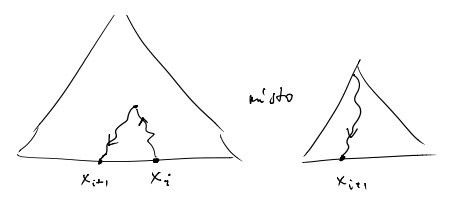
\includegraphics[width=0.6\textwidth]{img/asort.png}
\end{figure}


Předpokládáme, že při vkládání vrcholů je časově nejnáročnější nalezení místa pro něj, tedy že štěpění při opakovaném vkládání vychází amortizovaně $O(1)$ na operaci.

Celkový čas je tedy
$$T \leq 2\cdot \sum\limits_{i=1}^{n} log_a(|\{j\ |\ j\leq i; x_{i+1} < x_{j} \}|) + O(n)$$
kde první člen odpovídá hledání míst pro vkládané prvky a druhý výpisu posloupnosti (předpokládáme listy propojené spojovým seznamem). To lze díky konkávnosti logaritmu upravit na
\begin{align*}
T &\leq 2\cdot n\cdot \log_a\left(\frac{\sum\limits_{i=1}^{n} |\{j\ |\ j\leq i; x_{i+1} < x_{j} \}|}{n}\right) + O(n)\\
&= O(n\log\frac{F}{n})
\end{align*}
kde $F = \sum\limits_{i=1}^{n} |\{j\ |\ j\leq i; x_{i+1} < x_{j} \}|$ vyjadřuje celkový počet \uv{inverzí} v původní posloupnosti. Jistě platí $0 \leq F \leq n^2$, tedy máme zajištěnou i v nejhorším případě složitost $O(n\log n)$, v případě částečně setříděné posloupnosti je složitost lepší.

Existuje alternativní varianta algoritmu, v níž se místo pro nový prvek hledá vždy od nejpravějšího/nejlevějšího listu. Složitost vychází stejná.

Často se používají (2,3) stromy, protože mají nejmenší prostorové nároky a vzhledem k tomu, že nepoužíváme DELETE, nejsou ani tolik náročné na vyvažování (při obecném používání si ale právě z důvodu vyvažování vedou lépe (2,4) stromy).

\subsubsection{B-stromy}
Varianta používaná pro velká data uložená na disku, velikost uzlu odpovídá bloku paměti, aby se minimalizoval počet přístupů.

\textbf{Rozdíly: }
\begin{itemize}
	
	
	\item hodnoty uloženy i ve vnitřních vrcholech (namísto maxim z podstromů). 
	\item místo $a,b$ se volí pouze jediná hodnota, \textbf{řád stromu}: B-strom řádu $t$ je $\approx$ (t-1, 2t-1) strom (nebo (t,2t) strom nebo ($\lfloor t/2\rfloor$, t) strom -- záleží na konkrétní definici).
\end{itemize}

\textbf{Varianty}
\begin{description}
	
	
	\item[B+ stromy] Data \textbf{pouze} v listech (jako u obecných (a,b) stromů), sousední listy spojeny ukazateli. Používá např NTFS.
	
	\item[B* stromy] Zaplněnější vrcholy: dolní limit na zaplnění není 1/2 maxima, nýbrž 2/3 maxima. Při plném zaplnění se vrchol hned nerozpadá, nýbrž sdílí klíče se svým sousedem, teprve po zaplnění obou uzlů se tyto dva rozštěpí na 3.
\end{description}

\subsection{Červeno-černé stromy}
Binární vyhledávací strom, kde každý vrchol je obarven buď červeně nebo černě, a platí následující:
\begin{enumerate}
		
	
	\item listy jsou černé
	\item červené vrcholy mohou být syny pouze černých vrcholů
	\item všechny cesty z libovolně (pevně) zvoleného vrcholu $x$ do listu v podstromě $x$ mají stejný počet černých vrcholů
\end{enumerate}

Hodnoty jsou uloženy pouze ve vnitřních vrcholech, listy jsou ve skutečnosti pouze NULL pointery.

Dá se ukázat ekvivalence s (2,4) stromy, často se ČČ používají pro jejich implementaci. Nicméně ekvivalence platí zejména co se týče složitosti, samotná implementace je odlišná, zejména aktualizační operace pro ČČ a reprezentace vrcholů.
\begin{figure}[H]
	\centering
	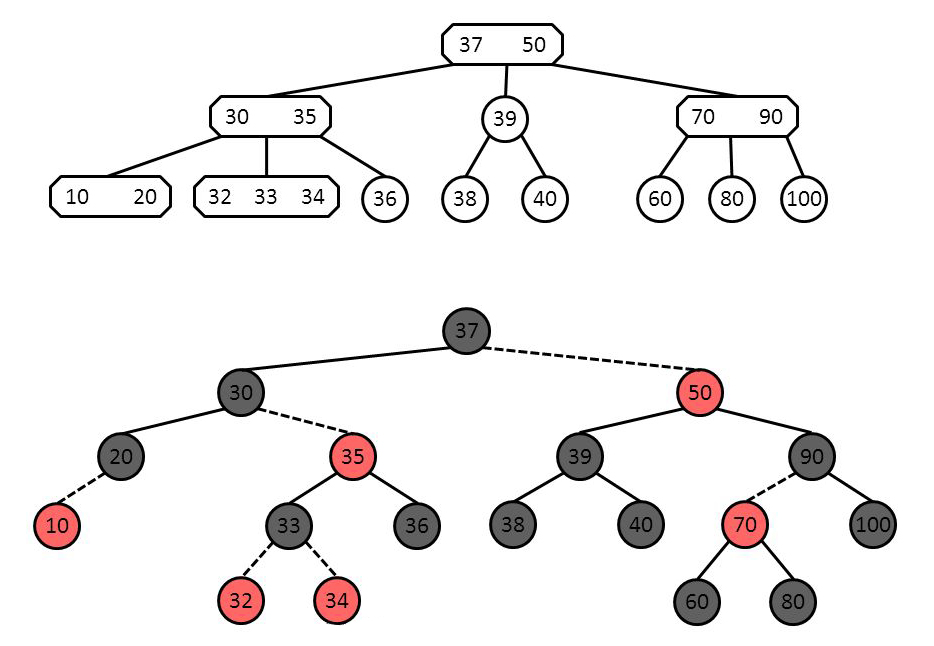
\includegraphics[width=0.44\textwidth]{img/rbtree_24tree.jpg}
	\label{rb24}
	\caption{Ekvivalence ČČ a (2,4) stromů na příkladu.}
\end{figure}

Používají se v knihovnách, např. STL v C++.

\begin{theorem}
	Červeno-černý strom obsahující $n$ prvků má hloubku $O(\log (n))$.
\end{theorem}
\begin{proof}
	Nechť $b$ je počet černých vrcholů na cestě z kořene do listu. Nejmenší možný strom obsahuje pouze černé vrcholy a má tedy $1 + 2 + 4 + \dots 2^{b-1} = 2^{b} - 1$ vrcholů. Největší možný strom sestává z cest, kde se střídají černé a červené vrcholy a má tedy $1 + 2 + 4 + \dots 2^{2b-1} = 2^{2b} - 1$ vrcholů. Tedy
	$$2^b - 1 \leq n \leq 2^{2b} -1$$
	$$b - 1 \leq \log_2 n + 1\leq 2b$$
	
	Hloubka stromu je nejvýše $2b \in O(\log_2 n)$
\end{proof}

\subsubsection{Operace INSERT(x)}
Najdeme místo pro nový vrchol jako v BVS. Přítomný černý NULLový list vymažeme, vložíme nový \textit{červený} vrchol $N$ obsahující $x$ a přidáme mu 2 černé NULLové syny. Podmínka 3 je v pořádku, mohla se ale porušit podmínka 2 (rodič $N$ je červený). Opravíme:
\begin{enumerate}
	
	\item \qquad 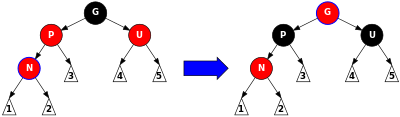
\includegraphics[scale=0.7]{img/rb_ins1.png}
	\item \qquad 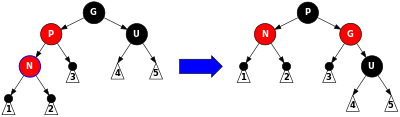
\includegraphics[scale=0.7]{img/rb_ins2.png}
	\item \qquad 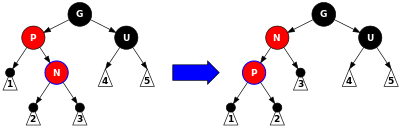
\includegraphics[scale=0.7]{img/rb_ins3.png}
\end{enumerate}


\subsubsection{Operace DELETE(x)}
Odstraňovaný vrchol $x$ má nejvýše jednoho neNULLového syna (má-li dva, prohodí se s maximem svého levého podstromu, ten má jistě nejvýše jednoho potomka). Je-li $x$ červený, OK. Je-li $x$ černý a jeho potomek červený, OK -- odstraníme, přebarvíme syna. Je-li $x$ černý a potomek také, je třeba opravovat. Odstraníme $x$ a potomka označíme jako \uv{dvojitě černého}. Tuto barvu navíc propagujeme nahoru, v nejhorším až do kořene, kde lze jednoduše odstranit. Rozbor případů viz třeba wikipedie.


\subsection{Splay stromy}
Splay stromy jsou variantou \textit{binárních vyhledávacích stromů} a jedná se o \textit{adaptivní} datové struktury. Základní myšlenkou je \textbf{udržovat často používané prvko blízko u kořene}. 

Cena za operaci může být až $O(n)$, ale amortizovaná cena za $k$ operací je $O(k\log n + n \log n)$ pro $n$ prvků uložených ve stromě.

\subsubsection{Operace SPLAY(x)}
Tato operace přesune prvek $x$ do kořene pomocí níže uvedených rotací. Aplikuje se po každé operaci FIND, INSERT, \dots

Používají se 3 typy rotací:
\begin{enumerate}
	
	\item \textbf{zig-zig}:
	
	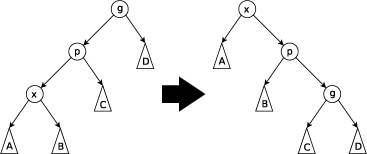
\includegraphics[height=100pt]{img/zigzig.png}
	
	\item \textbf{zig-zag}:
	
	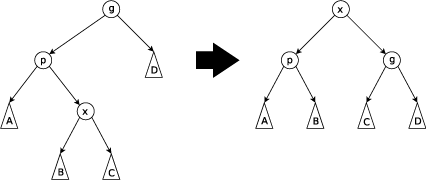
\includegraphics[height=100pt]{img/zigzag.png}
	
	\item \textbf{zig}:
	
	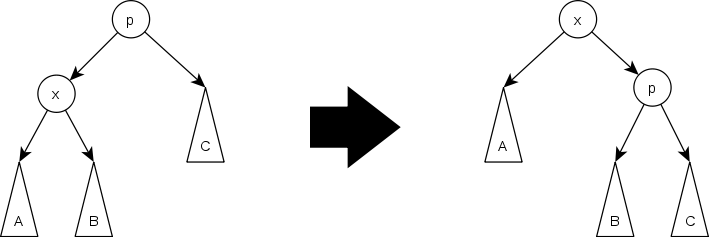
\includegraphics[height=70pt]{img/zig.png}
\end{enumerate}

Pokud to lze, používají se dvojrotace (zig-zig nebo zig-zag), jednoduchý zig slouží pro rotaci u kořene.

Časovou složitost rozebereme níže.

\subsubsection{Operace FIND(x)}
Funguje stejně, jako u klasického BVS, jen se na závěr ještě zavolá SPLAY(x). 

\subsubsection{Operace INSERT(x)}
Je několik variant:
\begin{enumerate}
	
	
	\item Proveď INSERT(x) stejně, jako u klasického BVS, poté proveď SPLAY(x).
	\item Proveď SPLIT(T,x) $\rightarrow T_1, T_2$, pak vytvoř nový strom s $x$ jako kořenem a $T_1, T_2$ jako levým resp. pravým synem.
	\item Varianta v Kouckého poznámkách: najdi $x$, nechť $u$ je poslední vrchol podél cesty k chybějícímu $x$. Proveď SPLAY(u) a vlož $x$ doleva/doprava pod kořen. Lze rozmyslet, že $u$ je buď bezprostředně menší nebo bezprostředně větší než $x$.
\end{enumerate}

\subsubsection{Operace DELETE(x)}
Opět více variant:
\begin{enumerate}
	
	
	\item Proveď DELETE(x) stejně, jako u klasického BVS, poté proveď SPLAY(parent(x)).
	\item Proveď SPLAY(X), smaž kořen a spoj dva vzniklé podstromy $L$ a $R$: najdi největší prvek $a$ v $L$, SPLAY(a), připoj $R$ pod $a$

\end{enumerate}

\subsubsection{Amortizovaná analýza}
Použijeme \textit{potenciálovou metodu} amortizované analýzy. Amortizovaný čas jedné operace je
$$t = a + \Phi(T') - \Phi(T)$$
kde $a$ je skutečný čas operace, $T$ je strom před operací, $T'$ strom po operaci a $\Phi(T)$ je potenciál stromu $T$, který definujeme takto:
$$\Phi(T) = \sum\limits_{x \in T} r(x), \quad \text{kde $r(x)$ je $\log_2(s(x))$ a $s(x)$ je počet vrcholů pod $x$} $$

Hodnota $r(x)$ vyjadřuje $rank$ uzlu $x$. Maximální možná hodnota je $\log_2(n)$, tj. $\Phi(T)$ je nejvýše $n\log_2(n)$. $\Phi(T)$ je tím nižší, čím je strom vyváženější.

Amortizovaný čas na $m$ operací je tedy:
\begin{align*}
t_1 + t_2 + \dots + t_m &= \sum\limits_{i=1}^{m} \left(a_i + \Phi(T_i) - \Phi(T_{i-1}) \right) \\
						&= \sum\limits_{i=1}^{m} a_i + \Phi(T_m) - \Phi(T_0) \\	
\end{align*}
Tedy \textit{reálný čas} na všechny operace ($\sum\limits_{i=1}^{m} a_i$) se od amortizovaného ($\sum\limits_{i=1}^{m} t_i$) liší nejvýše v rozdílu potenciálů před a po sekvenci operací, tj. $\Phi(T_m) - \Phi(T_0)$. Tento rozdíl může být nejvýše $n\log_2(n)$.

\begin{theorem}
Operace SPLAY(x) na libovolném vrcholu $x$ stromu $T$ zabere amortizovaný čas $\leq 3(r'(x) - r(x)) + 1$. Značení $r'(x)$ vyjadřuje rank vrcholu $x$ po operaci, $r(x)$ před operací.
\end{theorem}

\begin{proof}
Předpokládáme, že provedení rotace samotné zabere čas $t = 1$. 

Vždy se mění pouze rank zúčastnených vrcholů $x$, $p$ (parent) a $g$ (grandparent). Rozebereme jednotlivé případy:
\begin{enumerate}
	\item \textbf{\uv{zig-zig}}:
	 Jde o dvojrotaci, předpokládáme tedy cenu 2. Cena za operaci je
	 $$t = 2 + r'(x) - r(x) + r'(p) - r(p) + r'(g) - r(g)$$
	 Zjevně $r'(x) = r(g)$ (kořen před a po), tedy
 	 $$t = 2 - r(x) + r'(p) - r(p) + r'(g)$$
 	 Dále si všimneme, že $r(p) \geq r(x)$ a $r'(p) \leq r'(x)$, z čehož plyne
 	 \begin{align*}
	 	t 	&\leq 2 - r(x) + r'(x) - r(x) + r'(g)\\
	 		&= 2 + r'(x) - 2r(x) + r'(g)
 	 \end{align*}
	Nyní přichází klíčové pozorování. Uvažme výraz $2r'(x) - r(x) - r'(g)$. Ten musí být alespoň 2, neboť: 	 
	\begin{align*}
		2r'(x) - r(x) - r'(g) &= \log_2\left(\frac{s'(x)}{s(x)}\right) + \log_2\left(\frac{s'(x)}{s'(g)}\right)\\
							  &\geq \log_2\left(\frac{s'(x)}{\frac{s'(x)}{2}}\right) + \log_2\left(\frac{s'(x)}{\frac{s'(x)}{2}}\right)\\
							  & = 1 + 1 = 2
	\end{align*}
	Druhá nerovnost je dána díky $s'(x) \geq s(x) + s'(g)$ (viz obrázek) a protože díky vlastnostem logaritmu je nejnižší možná hodnota dosažena právě při volbě $s(x) = s'(g) = \frac{s'(x)}{2}$ (TODO lépe vysvětlit)

	Aplikujeme-li toto pozorování na předchozí nerovnici, dostaneme	
    \begin{align*}
	t 	&\leq 2 + r'(x) - 2r(x) + r'(g) \\
		&\leq (2r'(x) - r(x) - r'(g)) + r'(x) - 2r(x) + r'(g) \\
		&= 3(r'(x) - r(x)) \\
	\end{align*}
	
	\item \textbf{\uv{zig-zag}}:
	Postupujeme obdobně. Cena za operaci je 
	$$t = 2 + r'(x) - r(x) + r'(p) - r(p) + r'(g) - r(g)$$
	Zjevně $r'(x) = r(g)$ (kořen před a po) a $r(x) \leq r(p)$ a tedy
	$$t \leq 2 - 2r(x) + r'(p) + r'(g)$$
	
	Zopakujeme pozorování z předchozího případu, tentokrát však pro	$2r'(x) - r'(p) - r'(g)$. Stejně jako v předchozím případě plyne $2r'(x) - r'(p) - r'(g) \geq 2$ a tedy
	\begin{align*}
	t 	&\leq 2 - 2r(x) + r'(p) + r'(g) \\
		&\leq (2r'(x) - r'(p) - r'(g)) - 2r(x) + r'(p) + r'(g) \\
		&= 2(r'(x) - r(x)) \\
	\end{align*}
		
	
	
	\item \textbf{\uv{zig}}:
	
	Zde máme pouze $x$ a $p$. Cena za operaci je tedy
	$$t = 1 + r'(x) - r(x) + r'(p) - r(p)$$
	Jelikož rank $p$ jistě klesne ($r'(p) - r(p) < 0$) a rank $x$ naopak stoupne ($r'(x) - r(x) > 0$), platí
	\begin{align*}
	t 	&= 1 + r'(x) - r(x) + r'(p) - r(p)\\ 
		&\leq 1 + r'(x) - r(x) \\
		&\leq 1 + 3(r'(x) - r(x))\\
	\end{align*}

	
\end{enumerate}
\end{proof}

\begin{implication}
Posloupnost $m$ operací zabere amortizovaný čas 
$$m\cdot O(\log_2n) + O(n\log_2n)$$
\end{implication}
\begin{proof}
Díky předchozí větě a odhadu $\forall x : r(x) \leq \log_2(n)$ máme amortizovanou složitost na jednu operaci $O(\log_2 n)$, pro $m$ operací tedy $m\cdot O(\log_2n)$. Druhá složka $O(n\log_2n)$ je horním odhadem na rozdíl potenciálů před a po sekvenci operací.

Operace FIND, INSERT i DELETE lze provést tak, že sestávají z operace SPLAY a poté již jen několika akcí složitosti $O(1)$.
\end{proof}

To znamená, že pro $m \gg n$ (což bývá pravda) je složitost posloupnosti operací $O(m\log n)$, tj. amortizovaně $O(\log n)$ na operaci. 

Splay stromy si vedou dokonce ještě lépe, pokud je ditribuce operací nevyvážená.	

\begin{theorem}[entropy bound]
V \textit{optimálním} binárním vyhledávacím stromě, kde k prvku $x_i$ je přistupováno s pravděpodobností $p_i$, je očekávaná cena úspěšné vyhledávací operace 
$$\Theta(H) = \Theta\left(\sum_{i=1}^{n}-p_i \log p_i \right)$$
\end{theorem}
Tento vzorec odpovídá entropii rozdělení $p_i$. Pro uniformní přístupy vyjde $\log n$.

\begin{theorem}[static optimality]
Nechť $x_1, x_2, \dots, x_n$ je množina klíčů uložených ve splay stromě. Provedeme-li posloupnost vyhledávacích operací, v nichž každý klíč je vyhledáván aspoň jednou a každá operace je úspěšná, pak amortizovaná cena jedné operace je $O(1+H)$, kde $H$ je entropie pravděpodobnostního rozdělení přístupů. Cena $m$ vyhledávacích operací je $O(m+mH)$.
\end{theorem}
Tj. splay stromy jsou jen o konstantu horší, než optimální (tj. offline zkonstruované) stromy.


\subparagraph{Další zajímavé vlastnosti splay stromů}
\begin{theorem}[working set theorem]
Pokud provedeme $\Theta(n\log n)$ úspěšných vyhledávacích operací, pak amortizovaná cena jedné operace je $O(1+\log t)$, kde $t$ je počet operací od předchozího přístupu k danému prvku.
\end{theorem}
\begin{theorem}[sequential access theorem]
Pokud vyhledáme všech $n$ prvků ve splay stromě ve vzestupném pořadí, bude amortizovaná cena jedné operace $O(1)$.
\end{theorem}


\subsection{AVL stromy}
Binární vyhledávací strom je \textbf{AVL strom}, když pro každý uzel $x$ ve stromě platí 
$$|(\text{výška levého podstromu uzlu $x$}) - (\text{výška pravého podstromu uzlu $x$})| \leq 1$$

\begin{theorem}
Výška AVL stromu s $n$ vrcholy je $O(\log n)$.
\end{theorem}
\begin{proof}
Nechť $N(h)$ je minimální počet vrcholů stromu výšky $h$. Pak platí:
\begin{align*}
	N(0) &= 1 \\
	N(1) &= 2 \\
	N(h) &= 1 + N(h - 1) + N(h - 2)
\end{align*}
Zřejmě $N(h) \geq 2\cdot N(h-2)$ (protože $N(h-2) \leq N(h-1)$). 

Dále platí: $N(h) \geq 2^{\frac{h}{2}}$. To lze dokázat indukcí díky předchozímu pozorování:
$$N(h) \geq 2\cdot N(h-2) \geq 2\cdot 2^{\frac{h-2}{2}} = 2\cdot 2^{\frac{h}{2} - 1} = 2^\frac{h}{2}$$

Z toho dostaneme $h \leq 2 \log N(h)$
\end{proof}

Dotazovací operace mají tedy složitost $O(\log n)$.

Modifikující operace Insert a Delete pracují stejně jako na normálním BVS s případným dodatečným vyvážením pomocí rotací. Při Insert je třeba $O(1)$ rotací, při Delete to může být až $O(\log n)$. Celková složitost obou operací je $O(\log n)$.

\section{Haldy (regulární, binomiální).}
\subsection{Regulérní halda}
Halda je \textbf{stromová} datová struktura splňující tzv. \textbf{vlastnost haldy}: \textit{pokud je $B$ potomek $A$, pak $x(A) \leq x(B)$.} To znamená, že v kořenu je vždy prvek s nejnižším klíčem. Taková halda se pak označuje jako \textit{min heap}, opakem je je $max heap$. 

Regulární halda je co nejefektivněji zaplněná, přesněji všechny patra haldy jsou zcela zaplněné kromě nejspodnějšího, to je zaplněno zleva.

Typicky uvažujeme \textit{binární} neboli \textbf{2-regulární} haldu, ale obecně může být halda $k$-regulární.

\subsubsection{Reprezentace}
Haldy lze díky jejich zaplněnosti dobře implementovat pomocí pole, kde potomci uzlu na $n$-té pozici se nachází na pozici $2n$ a $(2n+1)$ (v případě binární haldy).
\begin{figure}[H]
	\centering
	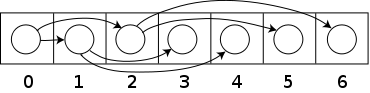
\includegraphics[scale=0.6]{img/heap.png}
\end{figure}

Libovolné pole prvků lze rychle převést na reprezentaci haldy -- lze ukázat, že to jde v $O(n)$ (operace HEAPIFY()):
\begin{proof}
Nechť $n = 2^{h+1} - 1$ pro nějaké $h$ (tj. stavíme kompletní strom hloubky $h$). Haldu stavíme od spodních pater. Budeme zkoumat, o kolik nejvýše pater musí prvky \uv{probublat}, aby se dostaly na správnou pozici
\begin{itemize}
	
	
	\item poslední patro (hloubka $h$) má $2^h$ prvků, žádný z nich ale nikam neprobublává
	\item patro $h-1$ má $2^{h-1}$ prvků, každý probublá nejvýše o 1 patro (do listu)
	\item patro $h-2$ má $2^{h-2}$ prvků, každý probublá nejvýše o 2 patro (do listu)
	\item \dots
\end{itemize}

Celkový počet operací je tedy:
\begin{align*}
T &\leq 2^h \cdot 0 + \leq 2^{h-1}\cdot 1 + 2^{h-2} \cdot 2 + \dots + 2^1 \cdot (h-1) + 2^0 \cdot h \\
 &=\sum\limits_{i = 0}^{h} 2^{(h-i)} \cdot i =\sum\limits_{i = 0}^{h} \frac{2^{h}}{2^i} \cdot i =2^h \cdot\sum\limits_{i = 0}^{h} \frac{i}{2^i}\\
\end{align*}
Jelikož řada $\sum\limits_{i = 0}^{\infty} \frac{i}{2^i}$ konverguje, lze ji shora omezit nějakou konstantou $C$ (lze ukázat $C = 2$) a tedy počet operací je $C\cdot 2^h$, tedy $O(n)$.
\end{proof}


\subsubsection{Operace}
\begin{itemize}
	
	
	\item \textbf{INSERT(x)}: $O(\log n)$
	
	 Prvek je přidán na konec posledního patra a poté se opraví halda, tj. prvek probublává směrem ke kořeni, dokud není opravena \uv{haldovitost}. Složitost je daná výškou haldy, která je $O(\log n)$
	
	\item \textbf{MIN()}: $O(1)$
	
	Vrátí vrchol haldy (bez mazání).
	
	\item \textbf{DELETE-MIN()}: $O(\log n)$
	
	Smaže vrchol haldy. Na jeho místo se přesune poslední prvek (nejpravější v posledním patře; poslední prvek pole) a opraví se halda: přesunutý prvek probublává z kořene směrem dolů, dokud není napravena \uv{haldovitost}.	
\end{itemize}

\subsection{Binomiální halda}
Motivace: chceme rychlejší INSERT(x).

\textbf{Binomiální halda} je ve skutečnosti množina více jednotlivých haldově uspořádaných stromů (obecných, ne binárních), každý velikosti $2^k$ pro nějaké $k$. Vždy si pamatujeme, ve kterém stromě aktuálně leží nejmenší prvek.

Existují 2 varianty:
\begin{enumerate}
	
	
	\item \textbf{zbrklá varianta} Pro každé $k$ existuje v haldě vždy nejvýše 1 strom velikosti $2^k$. Halda je implementována jako \textit{pole} odkazů na jednotlivé stromy, kde $i$-tý odkaz ukazuje na strom s velikostí $2^i$.
	Operace:
	\begin{itemize}
		
		
		\item \textbf{INSERT(x)}: $O(\log n)$, amortizovaně $O(1)$ (za jistých podmínek)
		
		Přidán nový haldový strom velikosti $1 = 2^0$ obsahující $x$. Aktualizuje se ukazatel na strom s nejnižším prvkem, je-li třeba.
		
		Opraví se struktura: dokud existují nějaké 2 stromy stejné velikosti $2^i$, spoj je do jednoho velikosti $2^{i+1}$. Vždy se přivěsí jeden strom pod kořen toho druhého jako nejpravější potomek. To tedy implikuje strukturu hald jednotlivých velikostí:
		\begin{figure}[H]
			\centering		
			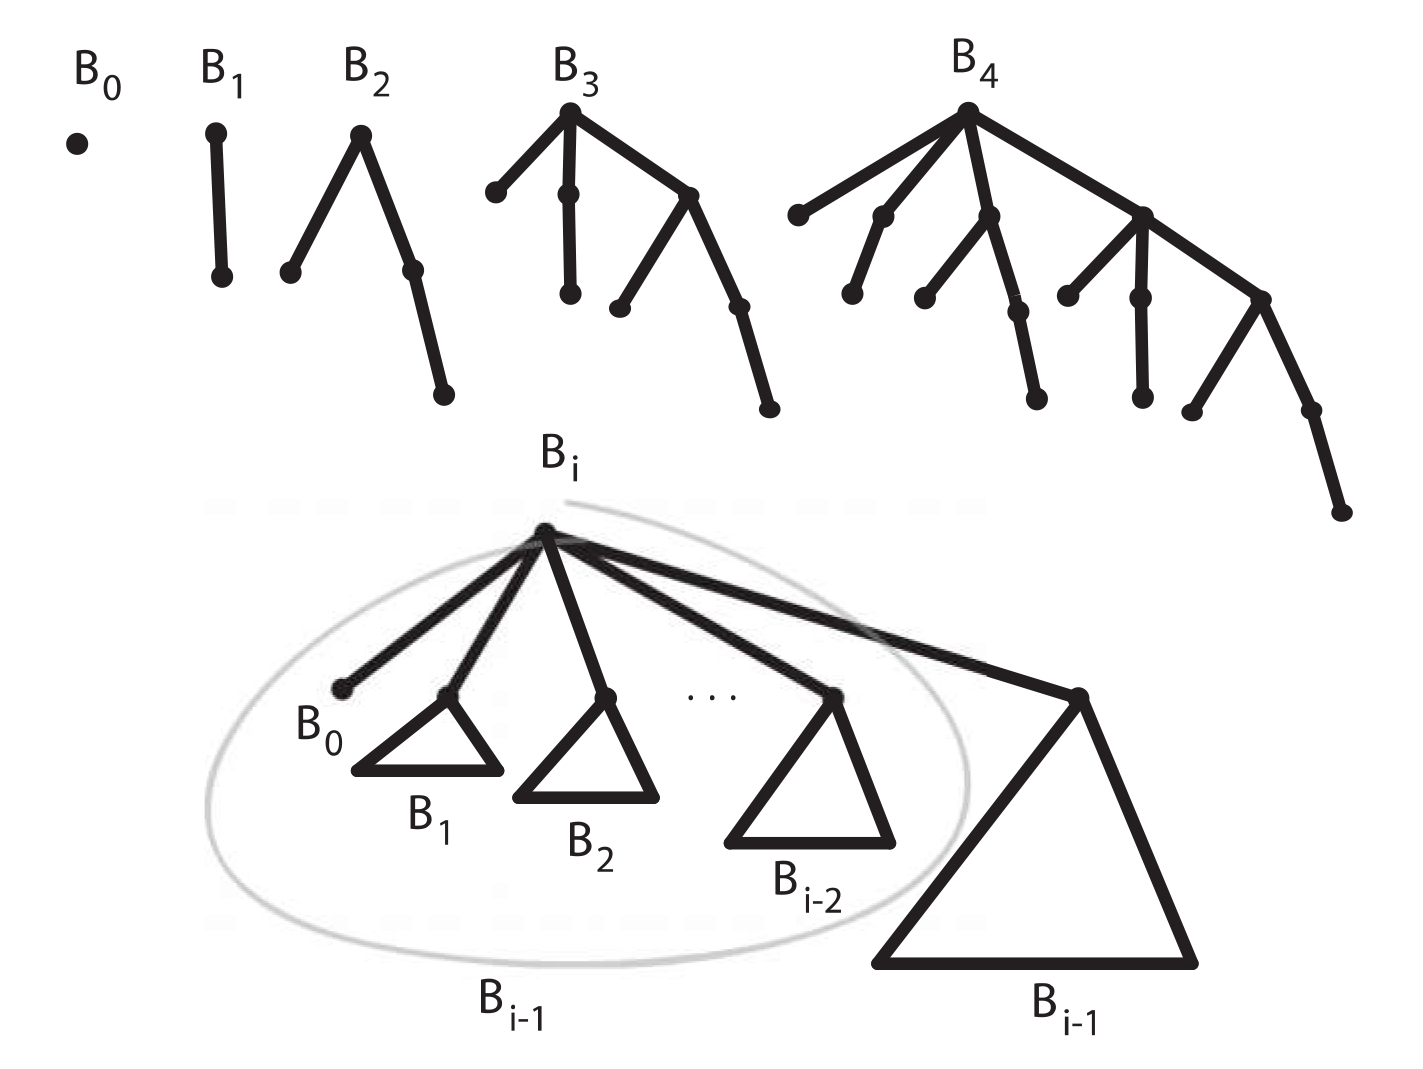
\includegraphics[scale=0.7]{img/binomial_heaps.png}
		\end{figure}

		Slévání funguje podobně jako \textit{binární sčítání}.
		
		\item \textbf{MIN()}: $O(1)$
		
		Vrátí vrchol stromu s minimálním prvkem (na který si pamatujeme ukazatel).
		
		\item \textbf{DELETE-MIN()}: $O(\log n)$
		
		Smaže kořen stromu s minimálním prvkem. Pokud má tento strom $2^i$ prvků, rozpadne se na stromy velikosti $2^0, 2^1, \dots 2^{i-1}$. Ty přidáme do haldy a podobně jako při INSERT opravíme haldu slučováním stromů stejné velikosti
	\end{itemize}
	
	INSERT trvá stále $O(\log n)$, nicméně vložení $n$ prvků do prázdné haldy trvá pouze $O(n)$ -- tedy amortizovaně máme INSERT v $O(1)$, pokud neprovádíme DELETE-MIN. Stačí rozmyslet, že slití stromů velikosti $2^i$ proběhne právě $\frac{n}{2^i}$-krát, dohromady
	$$\sum\limits_{i=0}^{\log n} \frac{n}{2^i} \leq n \sum\limits_{i = 0}^{\infty}\frac{1}{2^i} = 2n$$
	
	\item \textbf{líná varianta} Bez omezení na počet stromů stejné velikosti. Halda implementována jako \textit{spojový seznam} odkazů na stromy.

	Operace:
	\begin{itemize}
		
		
		\item \textbf{INSERT(x)}: $O(1)$
		
		Přidán nový haldový strom velikosti $1 = 2^0$ obsahující $x$. Aktualizuje se ukazatel na strom s nejnižším prvkem, je-li třeba. (Struktura se neopravuje.)
		

		\item \textbf{MIN()}: $O(1)$
		
		Vrátí vrchol stromu s minimálním prvkem (na který si pamatujeme ukazatel).
		
		\item \textbf{DELETE-MIN()}: $O(n)$, amortizovaně $O(\log n)$
		
		Smaže kořen stromu s minimálním prvkem. Pokud má tento strom $2^i$ prvků, rozpadne se na stromy velikosti $2^0, 2^1, \dots 2^{i-1}$. Ty přidáme do haldy a opravíme haldu slučováním stromů stejné velikosti, dokud to lze.
		
		V praxi: vytvoříme prázdné pole délky $\log n$ (což je maximální počet různých velikostí stromů), poté postupně bereme stromy ze spojového seznamu a vkládáme na správnou pozici. Je-li obsazena, sloučíme a vložíme o pozici výše, zde případně pokračujeme ve slučování. Jakmile vložíme všechny stromy, vytvoříme z pole opět spojový seznam.
	\end{itemize}

	DELETE-MIN je v nejhorším případě $O(n)$, amortizovaně však $O(\log n)$, což ukážeme potenciálovou metodou:
	
	Nechť $|T|$ značí počet stromů v haldě T, pak zvolme $\Phi(T) = C\cdot|T|$, kde $C$ je vhodná konstanta. Amortizovaná složitost operací:
	\begin{itemize}
		
		
		\item INSERT: $C + \Phi(T') - \Phi(T) = C + C = O(1)$ (přibyl 1 nový strom)
		\item MIN: $C + 0 = O(1)$ (žádný strom nepřibyl ani neubyl)
		\item DELETE-MIN: $C\cdot|T| + \Phi(T') - \Phi(T) = C\cdot|T| + O(\log n) - C\cdot|T| = O(\log n)$
		
		Počet stromů po slučování je nejvýše $\log n$.
	\end{itemize}
\end{enumerate}

\subsection{Fibonacciho halda}
Chceme přidat operaci DECREASE-KEY. Motivace: \textit{Dijkstrův algoritmus}. Šlo by prostě v případě porušení haldovitosti probublat ke kořeni v $O(\log n)$, my ale chceme $O(1)$.

Ostatní operace budou fungovat stejně, jako u líné binomiální haldy.

\subsubsection{Implementace}
Každý vrchol si udržuje své potomky ve spojovém seznamu, jejich počet a zda-li již o nějakého potomka přišel (označení). Celkově tedy z každého uzlu vedou ukazatele na: rodiče, sourozence a potomky.

\subsubsection{Operace DECREASE-KEY(v, k)}
Sníží hodnotu vrcholu $v$ o $k$. 
\begin{enumerate}
	
	
	\item Pokud je zachována haldovitost (tj. hodnota $v$ je stále větší než hodnota rodiče), hotovo. 
	\item Pokud je porušena haldovitost, odtrhni podstrom $v$ a zařaď ho do seznamu stromů. Byl-li označen, odznač.
	\begin{enumerate}
		
		
		\item Pokud rodič \textit{není} označen, označ jej. Hotovo.
		\item Pokud rodič \textit{je} označen (tj. již o nějakého potomka přišel), rekurzivně odtrhni rodiče.
	\end{enumerate}
\end{enumerate}

Každý rodič může přijít nejvýše o jednoho potomka, pak je sám odtržen. Kořen může přijít o libovolně mnoho synů.

Časová složitost amortizovaně $O(1)$ (i přestože může nastat kaskáda řezů). Ukážeme potenciálovou metodou: V předchozím případě jsme uvažovali potenciál $\Phi(T) = C \cdot |T|$. Upravíme jej na 
$$\Phi(T) = C \cdot(|T| + 2\cdot \#\text{označených vrcholů})$$
Jelikož pouze DECREASE-KEY operuje s označenými vrcholy, analýza ostatních operací zůstává stejná.

Nechť DECREASE-KEY provede $k$ řezů. V takovém případě dojde k odznačení $k$ vrcholů ($\Delta\Phi -= 2Ck$), přidání $k$ stromů do haldy ($\Delta\Phi += Ck$) a označení jednoho nového vrcholu \textbf{($\Delta\Phi += 2C$)}. Amortizovaná cena operace je tedy
$$C\cdot k + \Delta\Phi = C\cdot k - 2C\cdot k + C\cdot k + 2C = 2C = O(1)$$


\subsubsection{Analýza DELETE-MIN}
Jako \textit{řád} stromu označíme počet potomků kořene. Tato definice funguje i u binomiální haldy, tam dokonce platila korespondence, že strom řádu $k$ má velikost $2^k$. To u fibonacciho hald platit nebude, protože stromy budeme prořezávat.

Složitost $O(\log n)$ u binomiálních stromů vycházela z předpokladu, že maximální řád stromu je $O(\log n)$. To u Fibonacciho haldy není tak zjevné.

\begin{theorem}
Strom ve Fibonacciho haldě řádu $k$ má nejméně $F_{k+2}$ vrcholů, kde $F_i$ je $i$-té Fibonacciho číslo.
\end{theorem}
\begin{proof}
Indukcí. Stačí si nakreslit maximálně \uv{poškozený} strom, jeho podstromy jsou maximálně poškozené stromy nižších řádů.

Využíváme faktu $\sum\limits_{i = 1}^{n} F_i = F_{n+2} - 1$ (indukcí).
\end{proof}

\begin{theorem}
Pro každé $n \geq 3$ platí $F_n \geq (\frac{5}{4})^n$. 
\end{theorem}
\begin{proof}
Indukcí.
\end{proof}
Lze dokonce dokázat $F_n \geq \varphi^{(n-2)}$, kde $\varphi$ je zlatý řez.

\begin{theorem}
Maximální řád stromu ve Fibonacciho haldě je $O(\log n)$.
\end{theorem}
\begin{proof}
Plyne z předchozích 2 vět.
\end{proof}

\subsection{Další haldy}

\subsubsection{Pairing heap}
Fibonacciho haldy se považují za pomalé, kvůli vysokým konstantním faktorům u všech operací. \textbf{Pairing heap} je \uv{zjednodušení}, které udržuje téměř stejně dobrou asymptotickou složitost operací, ale v praxi je rychlejší.

Operace:
\begin{description}
	
	
	\item[MIN $O(1)$]: vrať kořen haldy
	\item[MERGE $O(1)$]: porovnej kořeny slučovaných stromů, zavěs větší pod menší
	\item[INSERT $O(1)$]: vytvoř nový strom pro vložený element a proveď MERGE s původní haldou
	\item[DECREASE-KEY (optional) $o(\log n)$]: odstraň strom zakořeněný v daném prvku, sniž klíč, proveď MERGE s původní haldou
	\item[DELETE-MIN: $O(\log n)$] odstraň kořen a sluč vzniklé podstromy. Různé strategie slučování.
\end{description}


\subsubsection{Brodal heap, strict Fibonacci heap}
Obě struktury mají stejnou složitost operací jako Fibonacci, ale zaručují je i \textbf{v nejhorším případě}. Jejich konstrukce je ale složitá a v praxi jsou nepoužitelné (podle slov autorů)


\section{Hašování, řešení kolizí, univerzální hašování, výběr hašovací funkce.}

\textit{Převzato z matfyz wiki (konvertováno pandocem).}
\subsection{Základní pojmy}

Základní motivací pro hashování je \emph{slovníkový problém}, kdy máme za úkol reprezentovat množinu $S$ prvků z nějakého univerza $U$ a provádět na ní následující operace:

\begin{itemize}	
	\item \textbf{MEMBER (FIND)} (je třeba, aby tato operace probíhala velmi rychle)
	\item \textbf{INSERT}
	\item \textbf{DELETE}
\end{itemize}

Triviální řešení: pole o velikosti $U$. To je však nepoužitelné v případě, že $|S| \ll |U|$ (a navíc $U$ může být neúnosně velké).

Použijeme \emph{hashovací funkci} $h : U \to \{0, \dots, m-1 \}$ a množinu $S$ reprezentuji \textbf{hašovací tabulkou} = polem s $m$ políčky tak, že $x\in S$ je uložen na indexu $h(x)$. Předpokládejme, že funkce $h$ se dá spočítat v čase
$O(1)$ -- jiné funkce nemají smysl.

Hlavní problém hašování jsou \textbf{kolize}: $x\neq y$, $h(x) = h(y)$. Existují různé strategie \textbf{řešení kolizí} a \textbf{předcházení kolizím} vhodnou volbou hašovací funkce (univerzální hašování, \dots)

Pro následující analýzy si označíme:

\begin{itemize}
	\item $n = |S|$
	\item $N = |U|$
	\item $m$ = velikost hašovací tabulky
	\item $\alpha=\frac{n}{m}$ = faktor zaplnění (\textit{load factor})
\end{itemize}

\subsection{Řešení kolizí}
Obecně jsou dvě strategie: \textit{zřetězení záznamů}, kdy je každý \textit{bucket} nezávislý a obsahuje ukazatel na nějaký spojový seznam; a \textit{otevřené adresování}, kdy jsou všechny prvky přímo v tabulce (ne nutně na nahašovaném poli). Mnoho variant je nějakou hybridní kombinací.

\subsubsection{Hashování se separovanými řetězci}
V tomto typu hashování se kolize řeší \emph{řetězením ve spojových seznamech}: pro každé políčko založíme zvlášť spoják všech prvků, které se do něj hashují. V nejhorším případě mají všechny prvky stejný hash a máme jen jeden spojový seznam.

Paměťová náročnost je pro každý seznam $O(1+l(i))$, kde $l(i)$ je délka toho seznamu.

Existují dvě varianty -- \textbf{neuspořádaná} a \textbf{s uspořádanými prvky} v řetězcích. Liší se jedině v očekávaném počtu testů pro neúspěšné hledání (když dojdu v řetězci za místo, kde by byl hledaný prvek, můžu skončit).

Pro odhad složitosti alogritmů předpokládáme, že:

\begin{itemize}
	\item Hashovací funkce $h$ rozděluje data rovnoměrně
	\item Sama reprezentovaná množina $S$ je náhodný výběr z $U$ s rovnoměrným rozdělením
\end{itemize}

Tyto předpoklady v praxi ale splněny být nemusí.

\paragraph{Očekávaná průměrná délka řetězců}

Pro odhad složitosti se počítá \textbf{očekávaná délka řetězců}. Označme délku $i$-tého řetězce jako $\mathbf{l}(i)$. To je náhodná veličina s \textit{binomickým rozdělením}, tj. $\mathbf{l}(i) \sim Bi(n,\frac{1}{m})$ a pravděpodobnost, že tento řetězec má délku $l$, odpovídá:

$$P(\mathbf{l}(i) = l) = \mathbf{}\binom{n}{l}\left(\frac{1}{m}\right)^{l}\left(1-\frac{1}{m}\right)^{n-l}$$

Toto je jen aproximace (pro nekonečnou velikost univerza i seznamů), pro případ, že $N\gg n^2 m$, ale lze použít. Očekávaná délka řetězce pak odpovídá střední hodnotě binomického rozdělení, tj. $n\frac{1}{m} = \alpha$. Jinými slovy, délka řetězce na libovolné pozici odpovídá celkovém faktoru zaplnění tabulky.

Rozptyl vyjde $\frac{n}{m}\left(1 - \frac{1}{m}\right)$, opět ze vzorce pro binomické rozdělení.

Očekávaná délka \textit{nejdelšího} řetězce je $\Theta(\frac{\log n}{\log\log n})$ (odvození je \textit{hodně} technické, lze nalézt ve Finkových slajdech).

\paragraph{Očekávaný počet testů (= porovnání) při hledání}
\begin{itemize}
\item \textbf{úspěšné hledání:} odpovídá průměrnému počtu testů provedených při \textit{vložení} každého z prvků, tj. (1 + očekávaná délka řetězce při každém vkládání):
$$\frac{1}{n}\sum_{i=0}^{n-1}\left(1+\frac{i}{m}\right) = 1 + \frac{1}{n}\frac{n(n-1)}{2m} = 1 + \frac{\alpha}{2} - \frac{1}{2m} \approx 1 + \frac{\alpha}{2}$$

\item \textbf{neúspěšné hledání:} v podstatě odpovídá průměrné délce řetězce, až na jeden člen navíc, který odpovídá situaci, kdy je řetězec prázdný -- i v tom případě totiž musím jeden test provést.

$$E(T) = P(\mathbf{l}(i) = 0) + \sum_l l P(\mathbf{l}(i) = l) = \left(1-\frac{1}{m}\right)^n + \frac{n}{m} \approx e^{-\alpha} + \alpha$$

S uspořádanými řetězci končím dřív: $e^{-\alpha}+1+\frac{\alpha}{2}-\frac{1}{\alpha}(1-e^{-\alpha})$.
\end{itemize}


\subsubsection{Hashování s přemísťováním/přesuny}
Nevýhodou separovaných řetězců je nutnost alokovat další paměť, to je neefektivní. Proto zavedeme do hashovací tabulky pomocné ukazatele a celé řetězce nacpeme přímo do ní (a zřetězené prvky prostě rozházíme na jiné adresy). Pro \emph{hashování s přemísťováním} se v tabulce uchovává navíc jednoduše odkaz na \emph{předchozí a následující prvek} řetězce. 

Při \textbf{INSERT}u na místo, kde už je nějaký prvek z \textit{jiného} řetězce, přehodíme tento cizí prvek jinam (přitom přesměrujeme příslušné ukazatele).

Při \textbf{DELETE} prvního prvku řetězce je nutné na jeho místo přesunout druhý (pokud existuje).

Očekáváný počet testů je stejný jako pro hashování se separovanými řetězci. Přemísťování v tabulce je ale náročnější než 1 test, proto jsou \textbf{INSERT} a \textbf{DELETE} pomalejší.

\subsubsection{Hashování se dvěma ukazateli}
Od předchozího se liší tím, že používá pouze dopředné odkazy a na poli $h(i)$ je odkaz BEGIN na pole tabulky, kde skutečně začíná řetězec prvků s hashem $h(i)$. Řetězec tak už nemusí začínat na indexu svého hashe.

Místo přesouvání prvků algoritmy mění BEGIN (ten je na $j$-tém políčku vyplněn, právě když existuje řetězec prvků s hashem $j$).

\begin{itemize}
	\item \textbf{INSERT} všechno vkládá na konec řetězce, zakládá-li nový, do
	BEGIN (na místě určené hashem) píše, kde se ve skutečnosti nachází.
	\item \textbf{DELETE} jen upravuje odkazy na následující, nebo BEGIN (pokud
smazáním zanikne řetězec).
\end{itemize}

Kvůli tomu, že řetězce začínají jinde než na svém místě, je počet testů o něco větší:

\begin{itemize}
	
	\item
	Úspěšné hedání:
	$1+\frac{(n-1)(n-2)}{6m^2} + \frac{n-1}{2m}\approx 1 + \frac{\alpha^2}{6} + \frac{\alpha}{2}$
	\item
	Neúspěšné hledání přibližně
	$1+\frac{\alpha^2}{2}+\alpha+e^{-\alpha}(2+\alpha)-2$.
\end{itemize}

\subsubsection{Srůstající (coalesced) hashování}
Srůstající hashování používá jen jeden ukazatel v hashovací tabulce navíc -- odkaz na další prvek NEXT. Řetězce tak mohou obsahovat hodnoty s různými hashy. Prvek $s$ vkládáme vždy do řetězce, který prochází $h(s)$-tým políčkem v tabulce.

Existují různé varianty:

\begin{itemize}
	\item standardní (bez pomocné paměti) -- LISCH, 	EISCH
	\item  s pomocnou pamětí -- LICH, VICH, EICH.
\end{itemize}

\paragraph{Bez pomocné paměti -- LISCH a EISCH}

\emph{LISCH} je \uv{late insertion}, tedy přidává se za poslední prvek řetězce. \emph{EISCH} (\uv{early insertion}) přidává za první prvek řetězce.

\begin{itemize}	
	\item \textbf{MEMBER} je stejný pro oba (jen projití řetězce po
	odkazech NEXT).
	\item \textbf{INSERT}: projití celého řetězce a pokud vkládaný prvek v řetězci není, vložení na libovolné volné místo v tabulce a připojení
	\begin{itemize}
		\item LISCH: na konec řetězce.
		\item EISCH: za první prvek (pokud je řetězec neprázdný).
	\end{itemize}
\end{itemize}

Algoritmy \textbf{DELETE} nejsou známy, kromě primitivních. Problémem je u nich zachování náhodného uspořádání prvků v řetězcích, které se předpokládá pro dodržení očekávaných časů operací. Je ale možné také prvky jen označit jako odstraněné a jejich místa použít při vkládání dalších (to ale zpomaluje hledání).

EISCH je kupodivu o něco rychlejší na úspěšné vyhledání (je větší pravděpodobnost práce s novým prvkem), očekávaný počet testů je stejný.

\paragraph{S pomocnou pamětí -- LICH, VICH, EICH}
V této variantě rozdělíme paměť na dvě části:
\begin{itemize}
	
	\item (hash-funkcí) přímo adresovatelná
	\item pomocná část (bez přístupu hash-funkcí) -- tzv. \uv{sklep}
\end{itemize}

Při kolizích nejdříve ukládáme do řádků z pomocné části, pak teprve do přímo adresovatelné, tedy oddalujeme srůstání řetězců. Chování se tak až do určitého okamžiku podobá separovaným.

Existují tři varianty podle chování algoritmu \textbf{INSERT}:

\begin{itemize}
	\item LICH vždy přidává na konec řetězce
	\item EICH v případě neprázdného řetězce vždy za 1. prvek 
	\item VICH na konec, pokud řetězec končí v pomocné paměti, jinak na místo, kde řetězec pomocnou paměť opustil (tj. chová se na pomocné paměti jako LICH a v přímo adresovatelné části jako EICH).
\end{itemize}

Algoritmy až na VICH se chovají stejně jako ve standardním srůstajícím hashování, rozhodující je výběr volného řádku pro vložení: např. \uv{vždy vyber z nejvyšší adresy} může zaručit používání pomocné paměti. 

Také tu není přirozené efektivní \textbf{DELETE}.

Na hledání volného řádku se v praxi hodí např. spojový seznam volných řádků.


\subsubsection{Lineární přidávání}
Nepoužívá ukazatele v hašovací tabulce. 

V případě kolize při \textbf{INSERT}u nalezne nejbližší vyšší volné políčko a vloží nový prvek tam. Předpokládáme \uv{cyklickou} paměť, tj. když dojdeme na konec, vkládáme od začátku.

Problémem je tvoření \emph{shluků} -- při velkém zaplnění se operace dost zpomalují. Také nepodporuje efektivní DELETE -- buď označit místo jako smazané nebo přehašovat. 

\emph{Očekávaný počet testů} je $\frac{1}{2}\left(1+\left(\frac{1}{1-\alpha}\right)^2\right)$ v
neúspěšném a
$\frac{1}{2}\left(1+\left(\frac{1}{1-\alpha}\right)\right)$ v
úspěšném případě (bez důkazu).

Variantou je přičítat konstantu vyšší než 1, tj. obecně $h(x) + ai$ (částečně zabraňuje shlukům) nebo použít \textbf{kvadratické přidávání}: $h(x) + ai + bi^2$.

\subsubsection{Dvojité hashování}

\emph{Dvojité hashování} je vylepšení předchozí metody tak, aby nevznikaly shluky. Výběr následujícího řádku bude závislý na předchozím, ale s rovnoměrným rozložením. Na to použiji \emph{druhou hashovací funkci} $h_2$.

Při operacích \textbf{INSERT} pak hledám nejmenší $i$ od $0$, že $(h_1(x) + i\cdot h_2(x)) \mod m$ je volné políčko, tj. postupně přičítám $h_2(x)$ a modulím. Stejný postup je i pro operaci \textbf{MEMBER}.

Je nutné, aby $h_2(x) \not | m$, tj. abych měl prosté posloupnosti (a z každého políčka tak mohl vést řetězec po celé tabulce). Idea, že iterace $h_2$ tvoří pro každé $x$ náhodnou permutaci paměťových míst, není úplně přesná, ale v praxi stačí, aby z $h_1(x) = h_1(y)$ plynulo, že $h_2(x)$ a $h_2(y)$ budou odlišné.

Funkce navíc musíme volit ``chytře'' (i lineární přidávání je spec. příp. dvojitého hashování, kdy $h_2 \equiv 1$). Pak tato metoda je znatelně rychlejší než lin. přidávání. Předpoklad náhodnosti použitý v teoretické analýze sice splnit nelze, ale přiblížit se mu ano.

\paragraph{Očekávaný počet testů}
Předpokládáme, že iterování funkce $h_2$ tvoří náhodné permutace (což, jak bylo řečeno, není úplně přesné). Počet testů označíme $C(m,n)$.

\begin{itemize}
	\item \textbf{neúspěšný případ:} Označme $q_i(n,m)$ pravděpodobnost, že při zaplnění $\frac{n}{m}$ je při INSERT(x) pro nějaké $x$ obsazeno prvních $i-1$ políček, kam bych ho mohl vložit. Potom
	$$q_i(n,m) = 
	\frac{n}{m}\cdot\frac{n-1}{m-1}\dots\frac{n-i+1}{m-i+1} = \frac{\prod_{j=0}^{i-1}(n-j)}{\prod_{j=0}^{i-1}(m-j)}$$
	a tedy $$q_i(n,m)=\frac{n}{m}q_{i-1}(n-1,m-1)$$
	
	Očekávaný počet testů je (předposlední rovnost plyne z rekurentního
	vztahu pro $q_j$, poslední krok dokázat indukcí):
	\begin{align*}
	C(n,m)&=\sum_{j=0}^n(j+1) (q_j(n,m) - q_{j+1}(n,m)) \\ 
	&=\sum_{j=0}^n(q_j(n,m)) = 1+\frac{n}{m} C(n-1,m-1)\\
	&= \frac{m+1}{m-n+1} \approx \frac{1}{1 - \alpha}
	\end{align*}
	
	\item \textbf{úspěšný případ} -- stejná metoda jako u dřívějších analýz, takže vychází:
	
	$$\frac{1}{n}\sum_{i=0}^{n-1}C(i,m)=\frac{1}{n}\sum_{i=0}^{n-1}\frac{m+1}{m-i+1}\approx\frac{1}{\alpha}\ln\left(\frac{m+1}{m-n+1}\right)\approx\frac{1}{\alpha}\ln\left(\frac{1}{1-\alpha}\right)$$
	
\end{itemize}

\subsubsection{Kukaččí hašování}
Používáme 2 hašovací funkce $h_1$ a $h_2$, prvek $x$ musí být uložen buď v přihrádce $h_1(x)$, nebo $h_2(x)$. V každé přihrádce je nejvýše jeden prvek.

Operace FIND a DELETE jsou triviálně $O(1)$.

Při operaci INSERT postupuj takto:
\begin{figure}[H]
	\centering
	\begin{minipage}{.7\linewidth}
		\begin{algorithm}[H]
			\caption{}
			\begin{algorithmic}[1]
				\If{$T[h_1(x)] = x$ or $T[h_1(x)] = x$}
					\State \textbf{return}
				\EndIf
				\State pos $\gets h_1(x)$
				\For{$n$ times}
					\If{$T[pos]$ empty}
						\State $T[pos] \gets x$
						\State \textbf{return}
					\EndIf
					\State swap($x,T[pos]$)
					\If{$pos = h_1(x)$}
						\State $pos \gets h_2(x)$
					\Else
						\State $pos \gets h_1(x)$
					\EndIf
				\EndFor
				\State rehash(); insert($x$)
			\end{algorithmic}
		\end{algorithm}				
	\end{minipage}
\end{figure}

Zaříznout je možno i dříve, cca po $\Omega(\log n)$ krocích.

Při rehashování náhodně vygenerujeme nové funkce $h_1, h_2$ a můžeme zvětšit velikost tabulky. Vložíme všechny prvky (pozor, tady může dojít k vnořenému rehashování -- pozor na ztrátu prvků!)


\paragraph{Analýza}
Kukaččí graf funguje dobře pro $m \approx 2.3n$. My budeme pracovat s grafy, pro něž platí $m \leq 2cn, c>1$. (\textit{Pozn.: Koucký používal $m = 6n$, tj. $c = 3$}).

Při analýze budeme pracovat s \textbf{kukaččím grafem}, kde 
\begin{itemize}
\item vrcholy jsou přihrádky tabulky
\item hrany jsou dvojice $(h_1(x), h_2(x)), \forall x \in S$	
\end{itemize}

\begin{theorem}
Nechť $S \subseteq U, |S| = n, m \leq 2cn, c>1$. Pravděpodobnost, že pro náhodně zvolené hašovací funkce $h_1, h_2$ jsou pozice $i,j$ spojeny cestou délky $k$, je nejvýše $\frac{1}{mc^k}$.
\end{theorem}
\begin{proof}
Induction on $k$:
\begin{enumerate}
	\item [$k=1$] For one element, the probability that it forms an edge $ij$ is $2/m^2$ . So, the probability that there is an edge $ij$ is at most $\frac{2n}{m^2} \leq \frac{1}{mc}$
	
	\item[$k > 1$] There exists a path between $i$ and $j$ of length $k$ if there exists a path from $i$ to $u$ of length $k - 1$ and an edge $uj$. For one position $u$, the $i-u$ path exists with probability
	$\frac{1}{mc^{k-1}}$. The conditional probability that there exists the edge $uj$ if there exists $i-u$
	path is at most $\frac{1}{mc}$ because some elements are used for the $i-u$ path. By summing
	over all positions $u$, the probability that there exists $i-j$ path is at most
	$$m\frac{1}{mc^{k-1}}\frac{1}{mc} = \frac{1}{mc^k}$$
\end{enumerate}
\end{proof}

\begin{theorem}
Nechť $S \subseteq U, |S| = n, m \leq 2cn, c>1$. Pravděpodobnost, že pro náhodně zvolené hašovací funkce $h_1, h_2$ obsahuje kukačkový graf cyklus je nejvýše $\frac{1}{2}$.
\end{theorem}
\begin{proof}
Pravděpodobnost cyklu délky $k$ vedoucího přes $i$ je dle předchozí věty $\frac{1}{mc^k}$. 

Pravděpodobnost cyklu libovolné délky je $\sum_{k>1} \frac{1}{mc^k} \leq \frac{1}{m}\frac{1}{c-1}$.

Pravděpodobnost, že nějaký vrchol $i$ je obsažen v cyklu je $m\frac{1}{m}\frac{1}{c-1} = \frac{1}{c-1}$
\end{proof}

\noindent\textbf{Důsledky:} Složitost operace Insert bez přehašování je $O(1)$. Pro $c > 2$ je počet přehašování při vkládání $n$ prvků $O(1)$. Amortizovaná složitost Insert včetně přehašování pro $c > 2$ je rovněž $O(1)$.

\subsubsection{Srovnání}\label{srovnuxe1nuxed}

Podle počtu testů:

\begin{table}[H]
	\centering
	\begin{tabular}{|l|l|l|}
	\hline
			& neúspěšné & úspěšné \\ \hline
		1. & separované uspořádané řetězce & separované (usp. i neusp.) řetězce,
		přemísťování \\ \hline
		2. & separované řetězce, přemísťování & dva ukazatele \\ \hline
		3. & dva ukazatele & VICH \\ \hline
		4. & VICH, LICH & LICH \\ \hline
		5. & EICH & EICH \\ \hline
		6. & LISCH, EISCH & EISCH \\ \hline
		7. & dvojité hashování & LISCH \\ \hline
		8. & lineární přidávání & dvojité hashování \\ \hline
		9. & & lineární přidávání \\ \hline
	\end{tabular}

\end{table}

\begin{itemize}
	
	\item
	VICH je při vhodném $\alpha$ lepší než hashování se dvěma
	ukazateli.
	\item
	Lineární přidávání se nedá použít pro $\alpha > 0.7$, dvojité
	hashování pro $\alpha > 0.9$.
	\item
	Separované řetězce a obecné srůstající hashování používají víc paměti,
	přemísťování a dvojité hashování zas víc času, tj. nelze říct, které
	je jednoznačně lepší.
\end{itemize}

\subsubsection{Implementační
	dodatky}\label{implementaux10dnuxed-dodatky}

\begin{itemize}
	
	\item
	Pro hledání volných řádků se většinou používá seznam (zásobník).
	\item
	Přeplnění se většinou řeší držením $\alpha$ v rozumném intervalu
	($\langle 1/4, 1\rangle$) a přehashováním do jinak velké tabulky
	($2^i\cdot m$) při pře- nebo podtečení
	\item
	V praxi se doporučuje přehashování odkládat (např. pomocnými
	tabulkami) a provádět při nečinnosti systému.
\end{itemize}

\textbf{DELETE} se ve strukturách, které ho nepodporují, řeší označením
políčka jako smazaného s možností využití při vkládání. V případě, že
polovina polí je blokovaná tímto způsobem, se vše přehashuje. Pro
srůstající hashování se toto používat nemusí, máme metody na zachování
náhodnosti rozdělení dat.

\subsubsection{Přehašování}
Při velkém zaplnění tabulky je u některých metod nutné přehašovat. V praxi se to dělá tak, že máme sadu hašovacích funkcí $h_0, h_1, \dots$, kde $h_0$ hašuje do tabulky velikosti $2^0 m = m$, funkce $h_1$ do tabulky velikosti $2^1m$, obecně $h_i$ hašuje do tabulky velikosti $2^i m$. 

Spolu s množinou $S$ si pak udržujeme i aktuální $i$ takové, že 
$$2^{i-2}m < |S| < 2^im$$
a S je aktuálně hašována funkcí $h_i$.

Při operacích INSERT a DELETE vždy kontrolujeme přetečení či podtečení této podmínky a případně zvětšíme/zmenšíme $i$ a přehašujeme.

Amortizovaná složitost přehašování je $O(1)$ (je ale vhodné jej dělat mimo dobu aktivního používání).




\subsection{Univerzální hashování}
Problém pevné hašovací funkce: pokud $N > mn$, tak pro každou hašovací funkci $h$ existuje $S \subseteq U$ velikosti $n$ taková, že $h$ hašuje všechny prvky $S$ do jedné přihrádky.

Budeme chtít sestrojit množinu funkcí $H : U \to M$, takový, že náhodně zvolená funkce $f \in H$ hešuje libovolnou množinu $S$ \uv{většinou dobře}. 

\emph{Definice}: Systém funkcí $H = \{ h_i; i \in I\}: U\to \{0,\dots,m-1\}$ je univerzální, pokud:
$$\forall x,y\in U, x\neq y: |\{i\in I; h_i(x)=h_i(y)\}|\leq \frac{|I|}{m}$$.
Tj. zaručuje se, že pro každé dva různé prvky má maximálně $1$ funkce kolizi.

Jiná formulace: pro náhodnou $h$ z $H$ a pro $\forall x,y \in U, x \neq y$ platí $$P[h(x) = h(y)] \leq \frac{1}{m}$$

\emph{Definice}: Systém funkcí $H = \{ h_i; i \in I\}: U\to \{0,\dots,m-1\}$ je $c$\emph{-univerzální}, pokud:

$$\forall x,y\in U, x\neq y: |\{i\in I; h_i(x)=h_i(y)\}|\leq \frac{c|I|}{m}$$.

Tj. zaručuje se, že pro každé dva různé prvky má maximálně $c$ funkcí kolizi.

Jiná formulace: pro náhodnou $h$ z $H$ a pro $\forall x,y \in U, x \neq y$ platí $$P[h(x) = h(y)] \leq \frac{c}{m}$$

\emph{Definice}: Systém funkcí $H = \{ h_i; i \in I\}: U\to \{0,\dots,m-1\}$ je $k$\emph{-nezávislý}, pokud pro náhodně zvolenou $h \in H$:

$$P[\bigwedge_{i=1}^{k} h(x_i) = z_i] = O(\frac{1}{m^k})$$

pro všechna po dvou různá $x_1, \dots, x_k \in U$ a všechna $z_1,\dots, z_k \in M$.

\textit{\textbf{V tomhle je bordel. Koucký používá k-univerzální záměnně s k-nezávislý, wiki taky, nicméně Fink a ještě nějaký jiný zdroj to má takhle.}}

\paragraph{Existence c-univerzálních
	systémů}\label{existence-c-univerzuxe1lnuxedch-systuxe9mux16f}

Předpokládejme, že universum má tvar $U=\{0,1,\dots,N-1\}$ kde
$N$ je nějaké prvočíslo a vezmeme funkce typu

$$h_{a,b}(x)=((ax + b) \mod N)\mod m$$

Jsou dobře použitelné, protože se dají počítat rychle. Protože $N$
je prvočíslo, můžeme pracovat v $\mathbb{Z}_N$, coz je těleso.
Rovnice $h_{a,b}(x)=h_{a,b}(y)$ je ekvivalentní s:

$$\exists i\in\{0,\dots,m-1\} \wedge \exists r,s\in\{0,\dots,\lceil\frac{N}{m}\rceil -1\} : (ax + b \equiv i + rm) \mod N \wedge (ay+ b \equiv i + sm) \mod N $$

Z Frobeniovy věty o jednoznačnosti řešení lineárních rovnic plyne, že
pro každé $r,s,i$ existuje jen jedna dvojice $a,b$, které
vyhovuje. Počet řešení soustavy je tedy omezený číslem
$m\cdot\lceil\frac{N}{m}\rceil^2$ ($i$:  $m$
hodnot, $r,s$:g $\lceil\frac{N}{m}\rceil$ hodnot pro daná
$x,y$).

Pak je systém $c$-univerzální pro
$c = \left(\lceil\frac{N}{m}\rceil\right)^2 / \left(\frac{N}{m}\right)^2$
a jeho velikost opdovídá $N^2$.

\paragraph{Vlastnosti}\label{vlastnosti}

Vyrobíme si pomocnou funkci

$$\delta_i(x,y)= \begin{cases}1 \mbox{ pro } h_i(x)=h_i(y), x\neq y \\ 0 \mbox{ jinak }\end{cases}$$

Chceme potom spočítat součet
$\delta_i(x,S)=\sum_{y\in S}\delta_i(x,y)$. Z výsledku vidíme
očekávanou délku řetězce pro libovolnou (jednu) množinu dat. Tohle pak
sečtu přes všechny mé hash-funkce a z $c$-univerzality dostanu

$$\sum_{i\in I}\delta_i(x,S)=\sum_{y\in S}\sum_{i\in I}\delta_i(x,y) \leq \sum_{y\in S,x\neq y} c\frac{|I|}{m} = \begin{cases} (|S|-1)c\frac{|I|}{m} & \mbox{ pro } x\in S \\ |S|c\frac{|I|}{m} & \mbox{ jinak }  \end{cases}$$

Z toho dopočítám (podělením $|I|$) horní odhad očekávaného
$\delta_i(x,S)$.

Výsledek: očekávaný čas operací \textbf{MEMBER}, \textbf{INSERT} a
\textbf{DELETE} v $c$-univerzálním hashování je
$O(1+c\alpha)$ (kde faktor naplnění $\alpha=\frac{|S|}{m}$).
Čas $n$ po sobě jdoucích operací na původně prázdné tabulce je
$O(n(1+\frac{c}{2}\alpha))$. To není lepší hodnota než mají
separované řetězce ($O(1+\alpha)$), ale u nich předpokládám
rovnoměrné rozdělení dat.

Výběr vhodné funkce není úplně jednoduchý, protože funkcí může celkem
být např až $N^2$, tj. nelze ho provést jednoduchým zavoláním
generátoru náhodných čísel, nýbrž např. náhodným vybráním každého bitu
indexu funkce. Proto je výhodné najít co nejmenší $c$-univerzální
systémy (viz
\protect\hyperlink{Dolnuxed_odhady_velikosti_univerzuxe1lnuxedch_systuxe9mux16f}{dále}).

\paragraph{Dolní odhady velikosti univ.
	systémů}\label{dolnuxed-odhady-velikosti-univ.-systuxe9mux16f}

Očíslujme hash-funkce z $I$ a induktivně definujme množiny
$U_i$ jako největší podmnožiny $U_{i-1}$ takové, že
$h_{i-1}(U_i)$ je jednoprvková. Platí
$|U_i|\geq \lceil \frac{U_{i-1}}{m}\rceil$, tedy
$|U_i|\geq\lceil\frac{N}{m^i}\rceil$ -- velikost těchto množin
klesá s logaritmem a
$|I|\geq \frac{m}{c}(\lceil\log_m N\rceil -1)$. Takže velikost
univ. systému roste alespoň úměrně logaritmu velikosti univerza.

\paragraph{Dolní odhad c}\label{dolnuxed-odhad-c}

\emph{5-univerzální systém}: Zvolme $t\in\mathbb{N}$ a k němu
vezměme $t$-té prvočíslo $p_t$ tak, že
$t\ln p_t\geq m\ln N$. Definujme systém funkcí
$H=\{g_{c,d,l}(x)|t<l\leq 2t, c, d\in\{0,1,\dots,p_{2t}-1\}\}$ kde
$((c(x\mod p_l)+d)\mod p_{2t})\mod m$. Zřejmě
$|H|=tp_{2t}^2$.

Odhadem $|G = \{(c,d,l); h_{c,d,l}(x)=h_{c,d,l}(y)\}|$, když si
množinu rozdělíme na
$G_1 = \{(c,d,l)\in G; x\mod p_l \neq y\mod p_l\}$ a
$G_2 =\{(c,d,l)\in G;x\mod p_l=y\mod p_l\}$, se dá dokázat, že
systém je 5-univerzální, za dalších podmínek i 3.25-univerzální.

\emph{Dolní odhad $c$}: Platí: $c>1-\frac{m}{N}$. Spočítáme
$\sum_{h\in H}\sum_{x,y\in U}\delta_h(x,y)$ -- pro pevnou
$h$ máme (z Cauchy-Schwarzovy nerovnosti,
$u_{i,h}=|\{x\in U,h(x)=i\}|$):

$$\sum_{x,y\in U}\delta_h(x,y)=\sum_{i=0}^{m-1}u_{i,h}(u_{i,h}-1)\geq \frac{(\sum_{i=0}^{m-1}u_{i,h})^2}{m}-N =\frac{N^2}{m}-N$$
Tedy
$\sum_{h\in H}\sum_{x,y\in U}\delta(x,y)\geq \frac{|H|N(N-m)}{m}$.
Zároveň platí
$\sum_{h\in H}\sum_{x,y\in U}\delta(x,y)\leq\sum_{x,y\in U}c\frac{|H|}{m}=N^2c\frac{|H|}{m}$,
což mi dává výsledek.

\subsection{Perfektní hashování}\label{perfektnuxed-hashovuxe1nuxed}

Základní ideou \emph{perfektního hashování} je nalézt hash-funkci, která
pro danou množinu $S$ nedělá žádné kolize, takže operace
\textbf{MEMBER} bude velice rychlá. Potom je nevýhoda, že nelze
přirozeným způsobem realizovat operaci \textbf{INSERT}, tj. v praxi se
nesmí moc často vyskytovat.

Tabulka by neměla být o mnoho větší než množina $S$ a funkce
$h$ rychle spočitatelná a její realizace nezabírat moc paměti
(tedy žádná zadávání tabulkou).

\paragraph{Definice}\label{definice}

\begin{itemize}
	
	\item
	Hashovací funkce $h$ je perfektní pro množinu $S$, pokud
	pro $\forall x,y\in S, x\neq y: h(x)\neq h(y)$
	\item
	Soubor funkcí $H:U\to \{0,\dots,m-1\}$ je
	$(N,m,n)$\emph{-perfektní}, pokud $\forall S\subseteq U$
	takové, že $|S|=n$ existuje $h\in H$ perfektní pro
	$S$.
\end{itemize}

\subsubsection{Odhady velikosti}\label{odhady-velikosti}

Každá funkce $h$ je perfektní pro
$\sum\{\prod_{j=0}^{n-1}|h^{-1}(i_j)|;0\leq i_0<\dots<i_{n-1}<m\}$
množin (sčítáme přes všechny množiny hashů $h(S)$ a pro každou z
nich uvažujeme všechny možnosti, jak mohla vzniknout). Z
Cauchy-Schwarzovy nerovnosti plyne, že tento výraz nabývá maxima, když
$\forall i: |h^{-1}(i)|=\frac{N}{m}$. Každá funkce je tedy
perfektní pro max. $\mathbf{}\binom{m}{n}(\frac{N}{m})^n$ množin.
Z toho plyne:

$$|H|\geq \frac{\mathbf{}\binom{N}{n}}{\mathbf{}\binom{m}{n}\left(\frac{N}{m}\right)^n}$$

Jiný odhad lze provést jako u $c$-univ. systémů s očíslovanými
funkcemi $|H|=\{h_1,\dots,h_t\}$. Používám induktivně definované
množiny $U_i$, kde $U_0 = U$ a $U_i$ je největší
podmnožina $U_{i-1}$, kde je zrovna funkce $h_i$ konstantní.
Dostáváme $|U_i|\geq \frac{|U_{i-1}|}{m}$, tj.
$|U_t| \geq \frac{N}{m^t}$, ale z perfektnosti plyne
$|U_t|\leq 1$. Dostáváme $t\geq \frac{log N}{log m}$.

\subsubsection{Existence}\label{existence}

Reprezentujme soubor funkcí $H=\{h_1,\dots,h_t\}$ na univerzu
velikosti $N$ pomocí matice $M(H)$ typu $N\times t$,
takže $M(H)_{x,i}=h_i(x)$, tj. v jednom sloupci jsou výsledky
jedné hashovací funkce pro všechny prvky univerza.

Pak žádná funkce z $H$ není perfektní pro množinu
$S\subset U$, když podmatice $M(H)$ tvořená řádky
příslušejícími prvkům $S$ nemá prostý sloupec. Takových matic je
maximálně (počet všech funkcí minus počet prostých, to celé krát
libovolné doplnění na $N$ řádek):

$$\left(m^n-\prod_{i=0}^{n-1}(m-i)\right)^t\cdot m^{(N-n)t}$$

Podmnožin $U$ velikosti $n$ je pak
$\mathbf{}\binom{N}{n}$, čímž vynásobeno mám počet matic
neodpovídajících $(N,m,n)$-perfektnímu systému. Všech matic je
$m^{Nt}$. Potom existuje $(N,m,n)$-perfektní systém, když:

$$\mathbf{}\binom{N}{n} \left(m^n-\prod_{i=0}^{n-1}(m-i)\right)^t\cdot m^{(N-n)t} < m^{Nt}$$
Příšernými kejklemi dostaneme podmínku existence
$t\geq n(\ln N)e^{\frac{n^2}{m}}$.

\subsubsection{Konstrukce funkce}\label{konstrukce-funkce}

Chceme splnit rychlou spočitatelnost a paměťovou nenáročnost.
Předpokládáme univerzum prvočíselné velikosti a funkce typu:

$$h_k(x)=(kx\mod N)\mod m$$

Označme $b_i^k=|\{x\in S; (kx\mod N)\mod m=i\}|$. Potom pokud
$h_k(x)$ není perfektní, pak nějaké $b_i^k =2$ a mám
$\sum_{i=0}^{m-1}(b_i^k)^2\geq n+2$.

Odhadnu výraz
$\sum_{k=1}^{N-1}((\sum_{i=0}^{m-1}(b_i^k)^2)-n) = \sum_{x\neq y\in S}\{k; 1\leq k<N, h_k(x)=h_k(y)\}$.
Z vlastností modula mám takových $k$ pro daná $x,y$ nejvýše
$2\lfloor\frac{N}{m}\rfloor =2\lfloor\frac{N-1}{m}\rfloor$.
Dostávám tedy odhad $2(N-1)\frac{n(n-1)}{m}$ a z něj vidím, že
existuje takové $k$, že
$\sum_{i=0}^{m-1}(b_i^k)^2\leq \frac{2n(n-1)}{m}+n$, tedy pro
tabulku velikosti $m > n(n-1)$ mám perfektní funkci.

Dá se dokázat trochu slabší předpoklad, že
$P(k;\sum_{i=0}^{m-1}(b_i^k)^2<\frac{3n(n-1)}{m}+n)\geq 1/4$,
který je základem pravděpodobnostního algoritmu.

Pak mám deterministický algoritmus, který pro $m=n(n-1)+1$ nalezne
perfektní $h_k$ v čase $O(nN)$ a pravděpodobnostní, který
pro $m=2n(n-1)$ najde perfektní $h_k$ v čase $O(n)$.
Mám tedy konstrukci perfektní hash-funkce, ta ale nesplňuje požadavek na
malou tabulku ($m=\Theta(n^2)$).

\paragraph{Menší tabulka}\label{menux161uxed-tabulka}

Zmenšíme-li velikost tabulky na $m = n$, bude výše uvedený algoritmus
schopný nalézt funkci, pro kterou platí $\sum (b_i^k)^2 < 3n$
($\sum (b_i^k)^2 < 4n$ v pravděpodobnostní variantě). Každou
kolizi pak můžeme ``rozstrkat'' perfektní funkcí nad miniaturní tabulkou
a celková velikost všech tabulek bude mnohem menší:

\begin{itemize}
	
	\item
	Vezmeme nalezenou funkci a najdeme všechny neprázdné množiny
	$S_i=\{s\in S;h_k(s)=i\}$
	\item
	Pro jim odpovídající $c_i=|S_i|(|S_i|-1)+1$ (dvojnásobek v
	pravděp. metodě) najdeme $k_i$ takové, že $h_{k_i}$ je
	perfektní funkce pro $S_i$ do tabulky velikosti $c_i$.
	\item
	Definujme $d_i=\sum_{j=0}^{i-1}c_j$, potom pokud
	$h_k(x)=l$, pak $g(x)=d_l+h_{kl}(x)$ je perfektní, její
	hodnota spočitatelná v čase $O(1)$ a hashuje do tabulky
	velikosti $O(3n)$ ($O(6n)$ s pravděp. případě), je
	naleznutelná v čase $O(nN)$ ($O(n)$) a pro její uložení do
	paměti jsou potřeba hodnoty $k$ a $k_i$, vyžadující
	$O(n\log N)$ paměti.
\end{itemize}

Pro výpočet $g(x)$ potřebuji 2 násobení, 2 modulo a 1 sčítání (pro
$d_i$ v paměti), tabulka má velikost
$\sum c_i\leq\sum (b_i^k)^2<3n$. Taková funkce ale stále nesplňuje
požadavek na málo paměti pro uložení.

\paragraph{\texorpdfstring{``Malá''
		funkce}{Malá funkce}}\label{maluxe1-funkce}

Víme, že pro $m\in\mathbb{N}$ je počet prvočísel, která ho dělí
$O(\frac{\log m}{\log\log m})$. Z toho úvahou o dělitelích čísla
$D=\prod_{1\leq i<j\leq n}(s_j-s_i)\leq N^{n^2}$ na
$n$-prvkové $S$ a vzorce hustoty prvočísel
$p_t\leq 2t\ln t$ dostanu, že existuje $p$ o velikosti
$O(\ln D)=O(n^2\ln N)$ takové, že $\phi_p(x)=x\mod p$ je
perfektní pro $S$.

Deterministické nalezení trvá $O(n^3\log n\log N)$ (test
perfektnosti každého systému je $O(n\log n)$). Proto použijeme
pravděpodobnostní algoritmus (mezi $4cn^2\ln N$ přir. čísly je
aspoň $1/2$ prvočísel, která vyhovují): nejdřív najde prvočíslo a
pak testuje perfektnost. Očekávaný počet testů je
$O(\ln(4cn^2\ln N))$, celková složitost algoritmu je pak
$O(n\log n(\log n+\log\log N))$. Najde zhruba až $2\times$
větší prvočíslo než deterministický.

Tuto funkci použijeme ke konstrukci výsledné hash-funkce:

\begin{enumerate}
	
	\item
	Nalezneme prvočíslo $q_0$, aby $\phi_{q_0}(x)=x\mod q_0$
	byla perfektní pro $S$
	\item
	Položíme $S_1=\{\phi_{q_0}(s)|s\in S\}$, pak najdeme prvočíslo
	$q_1\in \langle n(n-1)+1,2n(n-1)+2\rangle$
	\item
	K němu existuje $l\in \langle1,q_0-1\rangle$ takové, že
	$h_l(x)=((lx\mod q_0)\mod q_1)$ je perfektní pro $S_1$
	\item
	Položíme $S_2=\{h_l(s)|s\in S_1\}$ a najdeme perfektní $g$
	pro $S_2$ do tabulky s méně než $3n$ řádky (viz
	\protect\hyperlink{Menux161uxed_tabulka}{výše}, počítá se ale do
	univerza o velikosti $q_1$).
	\item
	Pak $f(x)=g(h_l(\phi_{q_0}(x)))$ je perfektní.
\end{enumerate}

Funkce $q_0$ je určena 1 číslem o velikosti $O(n^2\log N)$,
$h_l$ 2 čísly o velikosti $O(n^2)$ a $O(q_0)$,
$g$ je určená $n+1$ čísly o $O(q_1)$, tj. celkem
zadání vyžaduje $O(n\log n+\log n+\log\log N)$ paměti.



\section{Analýza nejhoršího, amortizovaného a očekávaného chování datových struktur.}
Uvažujeme dva \uv{zdroje}: \textbf{prostor} a \textbf{čas}. Využití obou zdrojů závisí na \textit{velikosti vstupních dat}. To je
\begin{itemize}
	\item \textit{formálně:} počet bitů nutných k zapsání vstupních dat
	\item \textit{neformálně:} počet nějakých elementárních entit na vstupu, např. počet vrcholů a hran grafu, počet měst pro TSP, počet prvků vstupní posloupnosti, kterou chceme setřídit atd.
\end{itemize} 
Většinou nám stačí neformální chápání velikosti vstupu, občas se ale hodí rigoróznější pohled -- například při definici číselných problémů a pseudopolynomiálních algorimů. Velikost vstupu značíme typicky $n$.

\textbf{Časová složitost} je pak nějaká funkce $f$ na $n$, která udává \textit{počet kroků algoritmu} v závislosti na $n$. Za \textit{krok algoritmu} považujeme triviální operace proveditelné v konstantním čase, např. sčítání, násobení, porovnání nebo přiřazení. Opět by šlo chápat definici rigorózněji a počítat třeba operace nějakého abstraktního stroje (Turingův, RAM).

\textbf{Prostorová složitost} je opět nějaká funkce $f$ na $n$, která udává \textit{velikost použité paměti} v závislosti na $n$. Jednotkou paměti může být třeba byte.

Typicky nás nezajímá přesný tvar funkce $f$ (tj. multiplikativní a aditivní konstanty), ale pouze do jaké 
\uv{třídy} funkce patří (lineární, kvadratická, exponenciální, \dots). 

\subsection{Asymptotická notace}
Intuitivně: zkoumá \uv{chování} algoritmu na \uv{velkých} datech, tj. nebere v úvahu multiplikativní a aditivní konstanty, pouze zařazuje algoritmy do \uv{kategorií} podle jejich skutečné časové složitosti.

Značení:
\begin{itemize}
	\item $f(n) \in O(g(n))$\quad \dots\quad $f(n)$ je \textbf{asymptoticky menší nebo rovna} $g(n)$
	$$\exists c > 0\ \exists n_0 > 0\ \forall n \geq n_0 : 0 \leq f(n) \leq c \cdot g(n)$$
	\item $f(n) \in \Omega(g(n))$\quad \dots\quad $f(n)$ je \textbf{asymptoticky větší nebo rovna} $g(n)$
	$$\exists c > 0\ \exists n_0 > 0\ \forall n \geq n_0 : 0 \leq c \cdot g(n) \leq f(n)$$
	\item $f(n) \in \Theta(g(n))$\quad \dots\quad $f(n)$ je \textbf{asymptoticky stejná jako} $g(n)$
	$$\exists c > 0\ \exists d > 0\ \exists n_0 > 0\ \forall n \geq n_0 : 0 \leq c\cdot g(n) \leq f(n) \leq d \cdot g(n)$$	
	\item $f(n) \in o(g(n))$\quad \dots\quad $f(n)$ je \textbf{asymptoticky ostře menší} $g(n)$
	$$\forall c > 0\ \exists n_0 > 0\ \forall n \geq n_0 : 0 \leq f(n) \leq c \cdot g(n)$$	
	\item $f(n) \in \omega(g(n))$\quad \dots\quad $f(n)$ je \textbf{asymptoticky ostře větší} $g(n)$
	$$\forall c > 0\ \exists n_0 > 0\ \forall n \geq n_0 : 0 \leq c \cdot g(n) \leq f(n)$$	
\end{itemize}



\subsection{Prostorová (paměťová) složitost reprezentované struktury}
Je důležitá, ale obvykle jednoduchá na spočítání a není šance ji vylepšit -- jedině použít úplně
jinou strukturu. 

\subsection{Časová složitost operací na datové struktuře}
\subsubsection{Časová složitost v nejlepším případě}
Chování v optimálních podmínkách. Analýza nejlepšího případu sama o sobě moc nevypovídá, ale může přinést odhad spodní hranice možného zlepšení.

\subsubsection{Časová složitost v nejhorším případě}
Její znalost nám zaručí, že nemůžeme být nepříjemně překvapeni (dobou běhu algoritmu). Hodí se
pro interaktivní režim -- uživatel sedící u databáze průměrně dobrou odezvu neocení, ale jediný
pomalý případ si zapamatuje a bude si stěžovat. 

Občas je těžké určit \uv{nejhorší} případ. Často se spíš uvažuje nejhorší možný chod algoritmu (nejvíce cyklů, \dots), aniž bychom znali konkrétní vstup, pro nějž by se takto choval (ani nemusí existovat). 

Bezpečná analýza, ale pesimistická. 

Za vylepšení nejhoršího případu obvykle platíme zhoršením průměrného případu.

Mnohdy může dobrá implementace vést k tomu, že k nejhorším případům nedochází (hašovací tabulky).

\subsubsection{Očekávaná časová složitost}
Je to vlastně vážený průměr -- složitost každého případu vstupních dat násobíme pravděpodobností
jeho výskytu a sečteme. Je zajímavá pro dávkový režim zpracování. Například Quicksort patří mezi
nejrychlejší známé třídící algoritmy, ale v nejhorším případě má složitost kvadratickou.


Mnoho problémů se špatnou složitostí nejhoršího případu se chovají dobře pro průměrné případy. To mnohdy vyhovuje (quicksort), někdy naopak chceme, aby \textit{všechny} instance byly \uv{špatné} (kryptografie).  


\subsubsection{Amortizovaná složitost}
\textbf{Amortizovaná analýza} je analýza nejhoršího případu pro \textbf{sekvenci operací}. Tím můžeme dostat těsnější odhad na složitost jedné operace (v rámci sekvence operací), než kdybychom analyzovali každou operaci zvlášť. To nás zajímá proto, že některé datové struktury mají takovou vnitřní organizaci, že na ní závisí složitost, a ta organizovanost se během posloupnosti operací mění. Nejhorší případ vlastně uklízí za následující nebo předchozí rychlé případy.

Existují 3 základní techniky pro amortizovanou analýzu:
\begin{enumerate}
	\item \textbf{agregovaná analýza:} Analyzuje celkový čas běhu pro posloupnost operací.
	\item \textbf{účetní (bankéřova) metoda:} Za operace musíme něco platit, za ty jednodušší méně, ušetřený kredit se použije na ty náročnější.
	\item \textbf{potenciálová metoda:} Definujeme vhodnou nezápornou \textit{potenciálovou funkci} (nebo prostě \textit{potenciál}), která charakterizuje \uv{uklizenost} struktury. Operace tuto hodnotu zvyšují nebo snižují.
\end{enumerate}

\noindent\textit{Příklady:}
\begin{itemize}
	\item \textbf{Binární čítač}
	
	Máme $n$-bitový čítač s operací Inkrement, která přičte jedničku -- tzn. nejzazší \textit{nulový bit se změní na 1} a všechny následující jedničkové bity se změní na nula. Počet změněných bitů je v nejhorším případě $n$. Zajímá nás, kolik bitů se změní při \textit{posloupnosti $k$ operací Increment} a jaký je tedy celkový čas posloupnosti operací.
	
	\begin{enumerate}
		\item \textbf{Agregovaná analýza:} Poslední bit se změní při každé operaci, tj. $k$-krát. předposlední bit se změní při každé druhé operaci, tedy v průměru $k/2$-krát. $i$-tý bit od konce se změní každých $2^i$ operací, tedy v průměrů k/$2^i$-krát. Celkový průměrný počet změn bitů je tedy $$\sum_{i=0}^{n}\frac{k}{2^i} \leq k \sum_{i=0}^{\infty} \frac{1}{2^i} = 2k$$
		
		Abychom získali \textit{horní} odhad, stačí vzít vždy horní celou část, tj. $i$-tý bit od konce se změní \textit{nejvýše} $\lceil k/2^i\rceil$-krát. Celkový počet změn je tedy \textit{nejvýše}
		$$\sum_{i=0}^{n}\left\lceil \frac{k}{2^i}\right\rceil \leq \sum_{i=0}^{k} (1 + \frac{k}{2^i}) \leq n + 2k$$
		\item \textbf{Účetní metoda:} Změna jednoho bitu stojí jeden žeton a na každou operaci dostaneme dva žetony. U každého jedničkového bitu v původní bitové sekvenci si \uv{uschováme} jeden žeton. Při inkrementu máme vynulování jedničkových bitů předplaceno. Oba žetony využijeme na jedinou změnu nulového bitu na jedničku a předplacení vynulování tohoto bitu. 
		
		V každém okamžiku tedy máme na všech jedničkách žetony, které se použijí na jejich případné vynulování. Každá operace stojí 2 žetony, tj. $2k$ žetonů celkem. Nejvýše $n$ žetonů jsme utratili na iniciální předplacení jedniček, dohormady tedy spotřebujeme nejvýše $n + 2k$ žetonů.
		
		\item\textbf{Potenciálová metoda:} Vhodnou potenciálovou funkcí je kupříkladu $\Phi = $\textit{počet jedničkových bitů}. Označíme $\Phi$ potenciál před operací a $\Phi'$ potenciál po provedení operace. Zajímá nás
		$$\text{amortizovaný čas} = \text{skutečný čas} + (\Phi' - \Phi)$$
		Nechť $j$ je počet jedniček vynulovaných při dané operaci. Pak skutečný čas operace je $j+1$ a změna potenciálů $(\Phi' - \Phi) = \Delta\Phi = (1-j)$. Amortizovaný čas je tedy
		$$\text{amortizovaný čas} = j+1 + 1-j = 2$$
		
		Celkový čas posloupnosti $k$ operací pak lze spočíst jako
		$$T = \sum_{i=1}^{k}\text{skutečný čas $i$-té operace} =  k\cdot\text{amortizovaný čas} + (\Phi_0 - \Phi_k) \leq 2k + n$$
		Poslední nerovnost plyne z $0 \leq \Phi \leq n$. Takovéto sečtení sumy $\sum_{i=1}^{k}(\Phi_{i-1} - \Phi_{i}) = \Phi_0 - \Phi_k$ se nazývá \textit{teleskopické vykrácení}.
	\end{enumerate}

	\item \textbf{Dynamické pole}
	
	Máme pole, do kterého přidáváme prvky i je z něj mažeme. Implementace používá statická pole pevné velikosti $p$. Je-li v poli již $n = p$ prvků (tj. je plné) a my chceme přidat prvek, vytvoříme nové pole velikosti $2p$, do něj zkopírujeme obsah původního pole a přidám prvek. Je-li $p = 4n$ a my chceme přidat prvek, zmenšíme pole na polovinu.
	
	\begin{enumerate}
		\item \textbf{Agregovaná analýza:} (neformálně) Zkopírování pole trvá $O(n)$. Po zkopírování je $n = p/2$ a k dalšímu kopírování dojde nejdříve po $n/2$ operacích Insert nebo Delete. Předpokládáme-li, že operace Insert a Delete jsou konstantní (pokud nedošlo ke kopírování), pak je amortizovaná složitost $O(1)$.
		
		(formálněji) Nechť $k$ je celkový počet operací a $k_i$ je počet operací mezi $(i-1)$ a $i$-tou realokací (platí $\sum_{i} k_i = k$). Při první realokaci se kopíruje nejvýše $n_0 + k_1$ prvků, kde $n_0$ je počáteční počet prvků. Při každé další realokaci se kopíruje nejvýše $2k_i$ prvků (plyne z toho, že pole se zdvojnásobuje, tj. nezvětšuje se o konstatní hodnotu). Celkem se tedy zkopíruje nejvýše
		$$n_0 + k_1 + \sum_{i \geq 2} 2k_i \leq n_0 + 2k$$
		prvků. Předpokládáme-li $O(1)$ na zkopírování jednoho prvku, pak dostáváme požadovanou amortizovanou složitost.
		
		\item\textbf{Potenciálová metoda:} 
		Definujeme následující potenciál
		$$
		\Phi = 
		\begin{dcases*}
		0 &\quad pokud $p = 2n$\\
		n &\quad pokud $p = n$\\
		n &\quad pokud $p = 4n$
		\end{dcases*}
		$$
		a zbylé případy lineární interpolací. Explicitně
		$$\Phi = 
		\begin{dcases*}
		2n - p &\quad pokud $p \leq 2n$\\
		\frac{p}{2} - n &\quad pokud $p > 2n$
		\end{dcases*}
		$$
		Minimální potenciál má tedy pole zaplněné právě z poloviny. 
		
		Prozkoumáme 3 případy:
		\begin{itemize}
			\item \textbf{Přidáváme či odebíráme prvek a \textit{ne}dochází k realokaci}. Skutečná cena operace je 1, rozdíl potenciálů je $\leq 2$ (důkaz rozborem případů). Amortizovaná cena je tedy $\leq 3$
			
			\item \textbf{Přidáváme prvek a dochází k realokaci.} To nutně znamená, že $\Phi = n$ a $\Phi' = 2$. Skutečná cena je $n + 1$ (realokace $n$ prvků + vložení 1 prvku). Amortizovaná cena je tedy
			$$A = (n+1) + (2-n) = 3$$
			
			\item \textbf{Odebíráme prvek a dochází k realokaci.} To nutně znamená, že $\Phi = n$ a $\Phi' = 1$. Skutečná cena je $n + 1$ (realokace $n$ prvků + odebrání 1 prvku). Amortizovaná cena je tedy
			$$A = (n+1) + (1-n) = 2$$
		\end{itemize} 
	
	\end{enumerate}
\end{itemize}



\section{Chování a analýza datových struktur na systémech s paměťovou hierarchií.}
\subsection{Paměťová hierarchie}

Pamť je v moderních počítačích hierarchická, od registrů v procesoru přes cache, RAM až po pevný disk. S rostoucí velikostí však roste i doba odezvy. 
\begin{figure}[H]
	\centering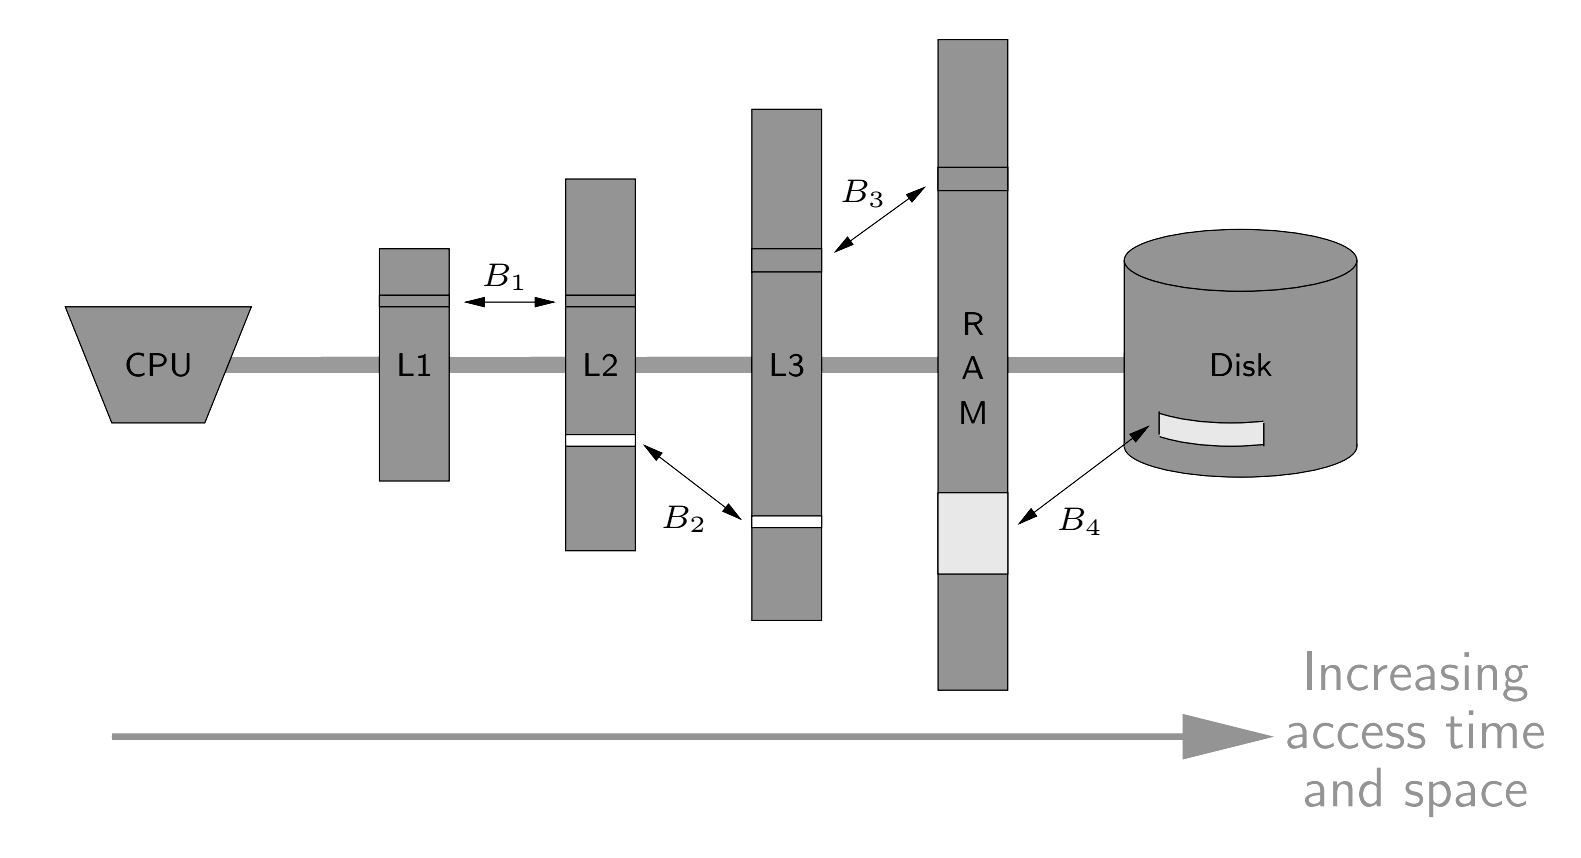
\includegraphics[]{img/memory.png}
	\caption{Paměťová hiearchie}
\end{figure}

\begin{table}[H]
	\centering
	\begin{tabular}{|l|r|r|}
		\hline
		& size & speed \\ \hline
		L1 cache & 32 KB & 223 GB/s \\ \hline
		L2 cache & 256 KB & 96 GB/s \\ \hline
		L3 cache & 8 MB & 62 GB/s \\ \hline		
		RAM 	& 32 GB & 23 GB/s \\ \hline		
		SDD 	& 112 GB & 448 MB/s \\ \hline		
		HDD 	& 2 TB & 112 MB/s \\ \hline		
		Internet & $\infty$ & 10 MB/s \\ \hline		
	\end{tabular}
	\caption{Příklad velikostí a rychlostí různých typů pamětí.}
\end{table}

\subsubsection{Zjednodušený model paměti}
\begin{wrapfigure}{r}{0.45\textwidth}
	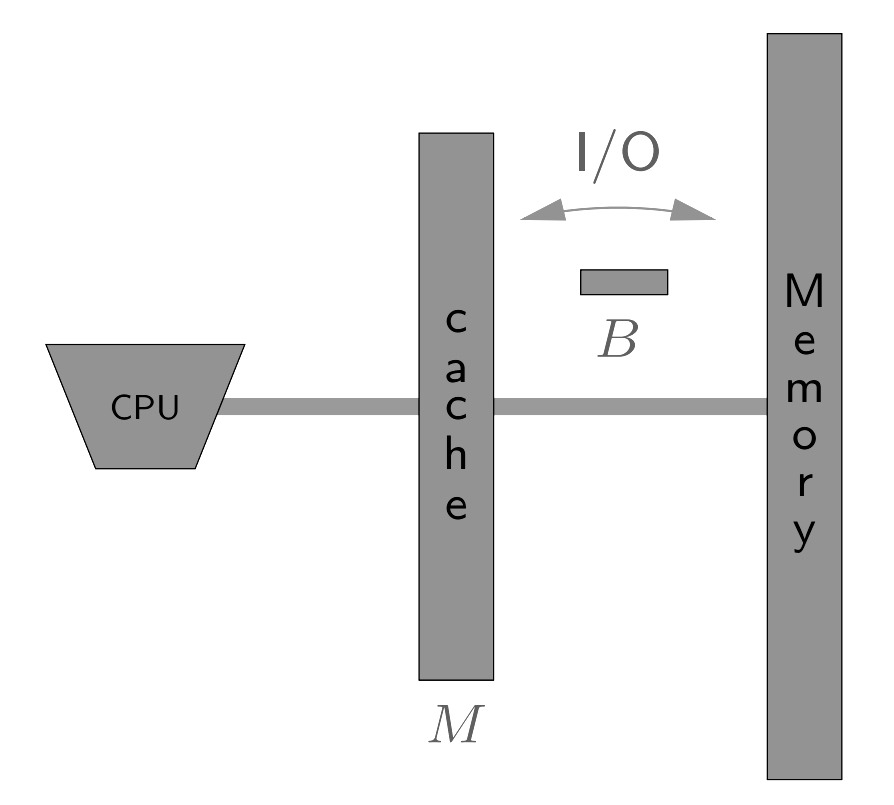
\includegraphics[width=0.4\textwidth]{img/memory_simple.png}
\end{wrapfigure}
Pro analýzu chování algoritmů a datových struktur v systémech s paměťovou hierarchií budeme uvažovat zjednodušený model paměti. Budeme mít pouze 2 úrovně: \textit{pomalý disk} a \textit{rychlou cache}.

Paměť je rozdělená na bloky velikosti $B$ (pro jednoduchost budeme předpokládat, že jeden prvek (integer, \dots) zabírá přesně jednotkový prostor, takže do jednoho bloku se vejde $B$ prvků). Velikost cache označíme $M$. Cache tedy obsahuje $P = M/B$ bloků. 

Procesor může přistupovat pouze k datům v cache. Paměť je plně asociativní, přičemž předpokládáme, že každý blok z disku může být uložený na libovolné pozici v cache. Data se mezi diskem a cache přesouvají po celých blocích. Naším cílem bude určit \textbf{celkový počet přenesených bloků}.

\subsection{Cache-aware a cache-oblivious algoritmy}
\textit{Pozn.: Otázka se ptá na \textbf{datové struktury} na systémech s paměťovou hierarchií, nikoliv algoritmy. Ke strukturám se taky dostaneme, ale v DS bylo tohle téma převážně o algoritmech. Proto je sem dáme taky.}

\textbf{Cache-aware} algoritmus je takový algoritmus, který \textbf{zná hodnoty $M$ a $B$} a podle nich nastavuje své parametry (např. velikost vrcholu B-stromu).

\textbf{Cache-oblivious} algoritmus je takový algoritmus, který efektivně funguje \textbf{bez znalosti $B$ a $M$}. 

Budeme zkoumat různé algoritmy prostřednictvím \textbf{cache-oblivious analýzy} -- tj. hodnoty $M$ a $B$ považujeme za neznáme a zkoumáme chování algoritmu, konkrétně počet přenesených bloků. 

\begin{itemize}
	\item \textbf{přečtení souvislého pole:} Máme pole zapsané v paměti v kuse, chceme přečíst úsek délky $n$. Počet přenesených bloků je nejvýše 
	$$\left\lceil \frac{n}{B}\right\rceil + 1$$
	
	\begin{figure}[H]
		\centering
		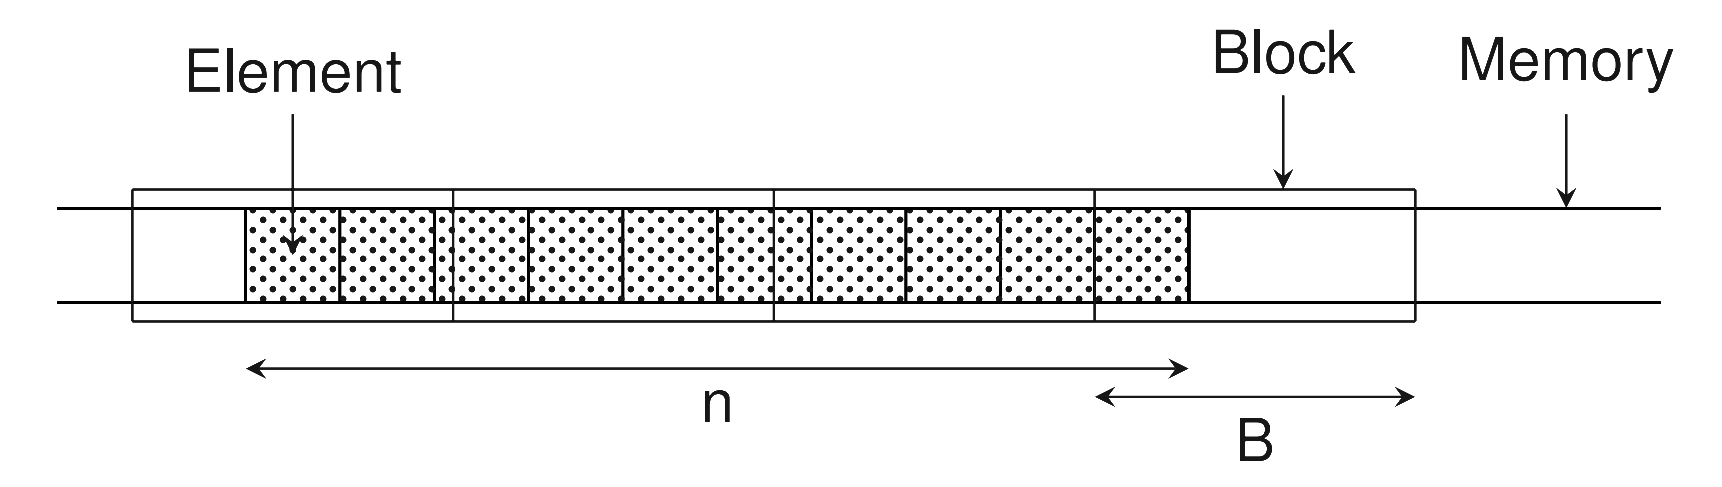
\includegraphics[scale=0.6]{img/cache_array.png}
	\end{figure}

	\item \textbf{binární vyhledávání v poli:} Celkem provedeme $\Theta(\log n)$ porovnání s hledaným prvkem (pro jednoduchost předpokládáme neúspěšné vyhledávání). Posledních $\Theta(\log B)$ prvků je uloženo nejvýše ve 2 blocích. Ostatní prvky jsou uloženy v po dvou různých blocích. Celkem je tedy přenesených bloků
	$$\Theta(\log n - \log B) = \Theta(\log \frac{n}{B})$$
	
	\item \textbf{průchod binární haldou uloženou v poli:} Analogicky jako předchozí případ, opět vyjde 
	$$\Theta(\log n - \log B) = \Theta(\log \frac{n}{B})$$
	\begin{figure}[H]
		\centering
		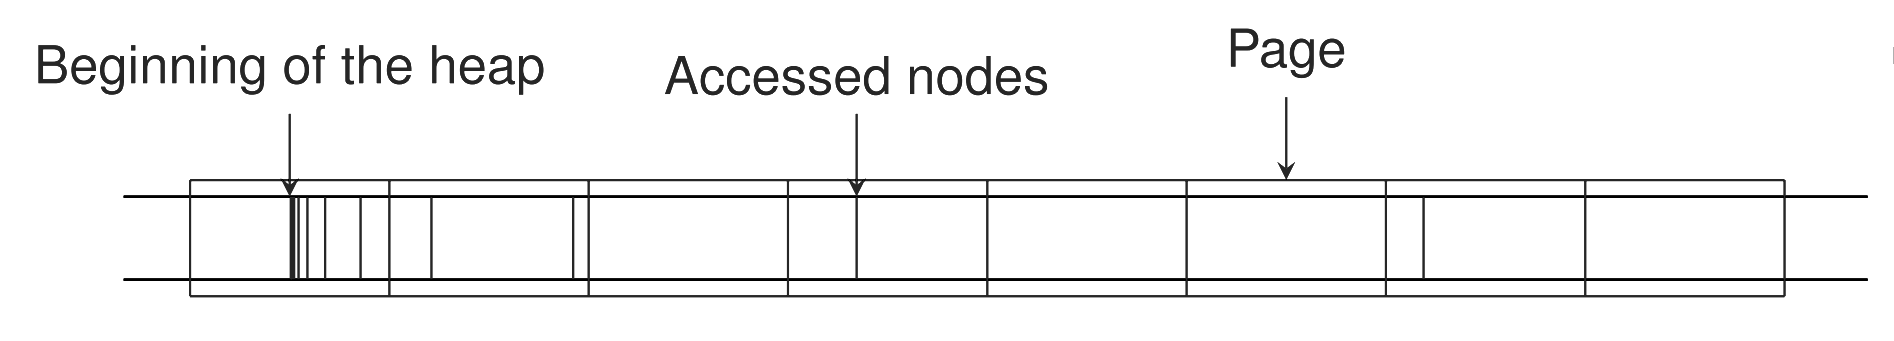
\includegraphics[scale=0.8]{img/cache_heap.png}
	\end{figure}
	
	\item \textbf{transpozice matice $n \times n$:} 
		Předpokládejme nejhorší možný případ, tj. $\frac{M}{B} < n$. Pokud je matice uložena po řádcích a do jednoho bloku se vejde nejvýše jeden řádek, tak to znamená, že se do cache nevejde celý sloupec matice. 
		\begin{enumerate}
			\item \textbf{naivní algoritmus}: 		
			Naivní implementace prochází matici po řádcích. 
			
			\begin{figure}[h]
				\centering
				\begin{minipage}{.7\linewidth}
					\begin{algorithm}[H]
						\caption{}
						\begin{algorithmic}[1]
							\For{$i = 1 \dots n$}
							\For{$j = 1 \dots n$}
							\State swap($A[i,j], A[j,i]$)
							\EndFor
							\EndFor
						\end{algorithmic}
					\end{algorithm}
					
				\end{minipage}
			\end{figure}
			
			Řekněme, že se řádek matice $A$ vejde do jednoho bloku. První řádek matice $A$ odpovídá prvnímu \textit{sloupci} matice $A^T$, přičemž každý prvek tohoto sloupce je v jiném bloku paměti. Pro transpozici prvního řádku tedy potřebujeme načíst do cache $1 + n$ bloků. Z předpokladu $\frac{M}{B} < n$ se však tolik bloků do cache nevejde, a tedy nutně musí nějaký blok z cache vypadnout. Pokud cache postupuje podle strategie LRU (\uv{least recently used}), pak tento vypadnutý blok odpovídá prvnímu řádku $A^T$. To znamená, že jakmile se dostaneme k druhému řádku $A$ a chceme umístit jeho první element $A_{2,1}$ do $A^T_{1,2}$, je již první řádek $A^T$ mimo cache a musí se znovu načíst. Toto se opakuje pro každý další element.
			
			Pokud by matice byla uložena po sloupcích (nebo pokud by transpozice postupovala po sloupcích), je situace podobná, avšak výpadky nenastávají při zápisu do $A^T$, nýbrž při čtení z $A$.
			
			Celkový počet přístupů do paměti je $\Omega(n^2)$.
			
			\item \textbf{cache-aware algoritmus}
			Funguje za předpokladu, že $M > B^2$ (tzv. \uv{tall cache}). Matici rozdělíme na podmatice $B \times B$ a použijeme následující algoritmus:
			\begin{figure}[h]
				\centering
				\begin{minipage}{.7\linewidth}
					\begin{algorithm}[H]
						\caption{}
						\begin{algorithmic}[1]
							\For{$i = 1; i < n; i += B$}
								\For{$j = i; j < n; j+= B$}
									\For{$ii = i; ii < min(k, i+B); i++$}
										\For{$jj = max(j,ii+1); jj < min(k, j+B); jj++$}
											\State swap($A[ii,jj], A[jj,ii]$)
										\EndFor
									\EndFor
								\EndFor
							\EndFor
						\end{algorithmic}
					\end{algorithm}				
				\end{minipage}
			\end{figure}
		
			Postupujeme tedy nikoliv po řádcích, ale po podmaticích $B \times B$. To nám zaručuje, že v rámci této podmatice nedochází k výpadkům paměti, jako v naivním algoritmu. První řádek této podmatice je zapsán nejvýše ve $2$ blocích, zapisujeme do $B$ bloků $A^T$, tedy $B+2$ bloků, což se do cache vejde. Přejdeme na druhý řádek, potřebujeme zapisovat do těch samých $B$ bloků, ty jsou stále v cache -- žádný výpadek. První řádek může již v klidu z cache vypadnout, bude-li třeba. I sloupce cílové podmatice mohou být uloženy až ve 2 blocích, celkem tedy načteme $4B$ bloků (bez výpadků). Podmatic je $(n/B)^2$, celkem tedy $$4B \cdot \left(\frac{n}{B}\right)^2 = 4\frac{n^2}{B} = O\left(\frac{n^2}{B}\right)$$
			
			Algoritmus pracuje s hodnotou $B$, je tedy cache-aware.
			
			\item \textbf{cache-oblivious algoritmus} Rekurzivní algoritmus. Matici $A$ rozdělíme na submatice
			$$A = 
			\begin{pmatrix}
			A_{11} & A_{12} \\
			A_{21} & A_{22}
			\end{pmatrix}
			\qquad
			A^T = 
			\begin{pmatrix}
			A_{11}^T & A_{21}^T \\
			A_{12}^T & A_{22}^T
			\end{pmatrix} 
			$$
			
			Rekurzivně transponujeme menší a menší podmatice, až se v nějakém $i$-tém kroku dostaneme na velikost $n_i$, která se již vejde do paměti, tj. $n_i \leq B \leq 2n_i$. Transponování v rámci této matice má stejné vlastnosti, jako v případě $B\times B$ matice u cache-aware algoritmu -- tj. nedochází k výpadkům a celkem je třeba načíst $4n_i \leq 4B$ bloků. Celkem máme $n/n_i$ těchto sumbatic, takže počet přenesených bloků je nejvýše
			$$\left(\frac{n}{n_i} \right)^2 \cdot 4n_i \leq \frac{8n^2}{n_i} = O\left(\frac{n^2}{B}\right)$$
			
			To je stekný výsledek, jako v předchozím případě. Tento algoritmus však již nezávisí na $B$ a je tedy cache-oblivious.
			
			\begin{figure}[h]
				\centering
				\begin{minipage}{.7\linewidth}
					\begin{algorithm}[H]
						\caption{}
						\begin{algorithmic}[1]
							\Function{transposeOnDiagonal}{$A$}
								\If{matice je \uv{malá}}
								\State Transponuj A triviálně
								\Else
									\State $A_{11}, A_{12}, A_{21}, A_{22} \gets$ souřadnice podmatic
									\State transposeOnDiagonal($A_{11}$)
									\State transposeOnDiagonal($A_{22}$)
									\State transposeAndSwap($A_{12}, A_{21}$)
								\EndIf
							\EndFunction
							
							\Function{transposeAndSwap}{$A, B$}
								\If{matice je \uv{malá}}
									\State Prohoď $A$ a $B$ a transponuj triviálně
								\Else
									\State $A_{11}, A_{12}, A_{21}, A_{22}, B_{11}, B_{12}, B_{21}, B_{22} \gets$ souřadnice podmatic
									\State transposeAndSwap($A_{11}, B_{11}$)
									\State transposeAndSwap($A_{12}, B_{21}$)
									\State transposeAndSwap($A_{21}, B_{12}$)
									\State transposeAndSwap($A_{22}, B_{22}$)
								\EndIf
								
							\EndFunction
						\end{algorithmic}
					\end{algorithm}				
				\end{minipage}
			\end{figure}
		\end{enumerate}
		\item \textbf{násobení matic} Velice podobný princip jako transpozice.
		\item \textbf{mergesort (binární):} Pokud $n \leq M/2$, tak se vejdeme do cache (polovina cache se použije pro vstupní pole, polovina pro slité). Přenášíme $2n/B + O(1)$ bloků.
		
		Pokud $n > M/2$: nechť $z$ je maximální velikost pole, které může být setříděno v cache (pro jednoduchost předpokládáme, že velikost polí v jedné úrovni cache jsou stejná), tzn. dvě pole velikosti $z/2$ mohou být slity v jedno pole velikosti $z$. Platí $z \leq M/2 < 2z$. Slití jedné úrovně vyžaduje $2\frac{n}{B} + 2\frac{n}{z} + O(1) = O(\frac{n}{B})$ přenosů (přečtení všech prvků + rezerva pro nezarovnané bloky). Celkový počet přenesených bloků je $O(\frac{n}{B})(1+\log_2\frac{n}{z}) = O(\frac{n}{B}\log_2\frac{n}{M})$.
		
		\item \textbf{funnel-sort} Chceme dostat $O(\frac{n}{B}\log_{\frac{M}{B}}\frac{n}{M})$ (lze ukázat, že to je dolní mez pro cache oblivious třídící algoritmy). Funnelsort rozdělí data na $N^{\frac{1}{3}}$ částí o velikosti $N^{\frac{2}{3}}$, ty rekurzivně setřídí a slije pomocí $N^{\frac{1}{3}}$-mergeru. 
		
		Obecný \textbf{$k$-merger} je stromovitá struktura bufferů, která slije $k$ vstupních bufferů do jediného výstupního. Stuktura viz obrázek \ref{merger}.
		
		Lze dokázat že za předpokladu tall cache je funnelsort optimální, tj. provede $O(\frac{n}{B}\log_{\frac{M}{B}}\frac{n}{M})$ přístupů do paměti.
		\begin{figure}[H]
			\label{merger}
			\centering
			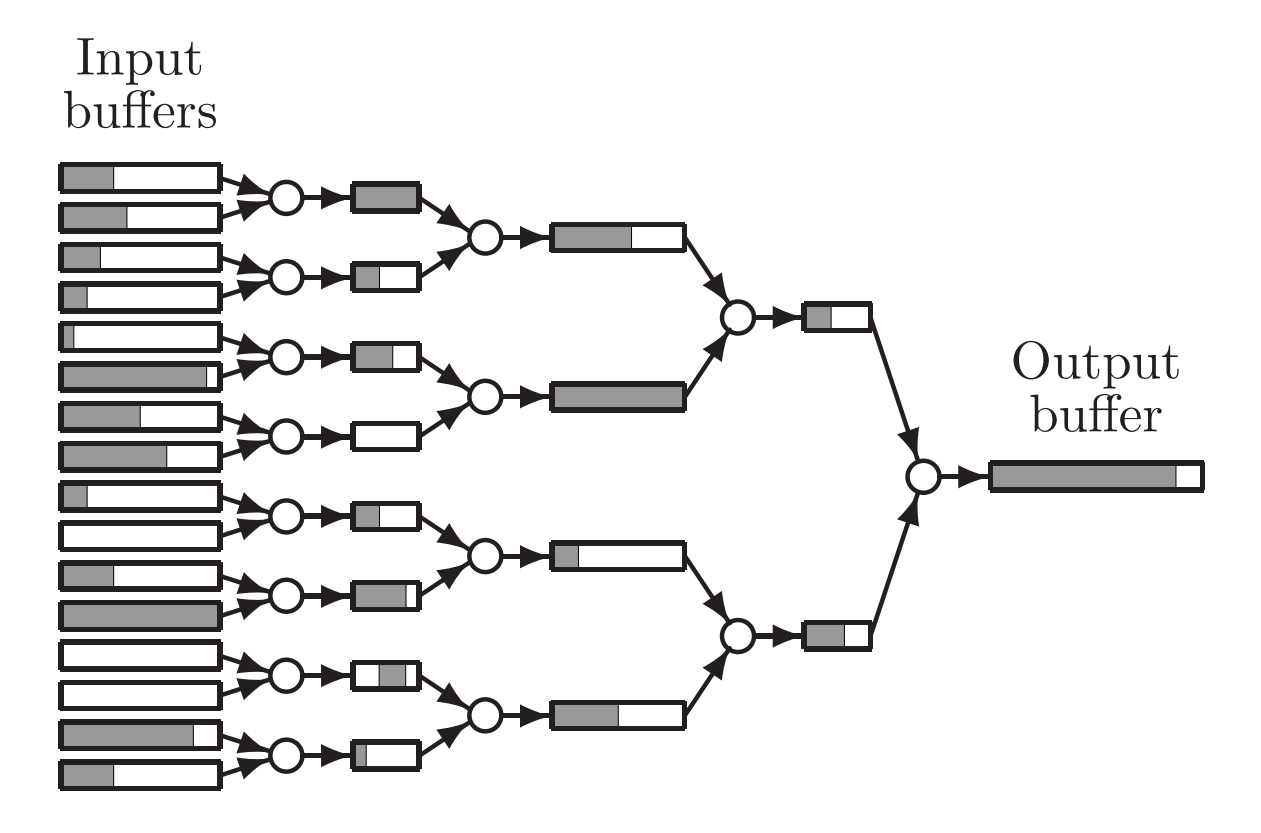
\includegraphics[]{img/kmerger.png}
		\end{figure}
\end{itemize}




\subsection{Cache-aware a cache-oblivious datové struktury}
Budeme chtít sestrojit efektivní reprezentaci \textbf{binárního stromu}.
\begin{itemize}
\item \textbf{Klasický binární strom (pomocí ukazatelů)}: co uzel, to jiný blok $\Rightarrow \log (n)$ přístupů do paměti.

\item \textbf{Binární halda:} $\Theta(\log(n) - \log(B))$

\item \textbf{B-strom:} uzly velikosti $B$, výška stromu je $\Theta(\log_B(n))$, při průchodu k listu se načte $\Theta(\log_B(n))$ bloků. Nicméně je to cache-aware struktura (a navíc jsme chtěli binární strom).

\textbf{van Emde Boas rozložení:} Rozsekneme strom v polovině výšky (tj. $h/2 = \log_2(n)/2$), vzniklé podstromy mají velikost $\sqrt{n}$. Do paměti uložíme v pořadí shora a zleva (viz obrázek). Rekurzivně rozdělujeme dále až do jisté úrovně, kdy podstrom výšky $z$ již vejde do cache. Platí $z \leq \log_2 B \leq 2z$.  Nyní počet podstromů výšky $z$ na cestě z kořene do listu je $$\frac{h}{z} \leq \frac{2\log_2 n}{\log_2 B} = 2\log_B(n)$$
Počet načtených bloků je tedy $\Theta(\log_B n)$.

\begin{figure}[H]
	\centering
	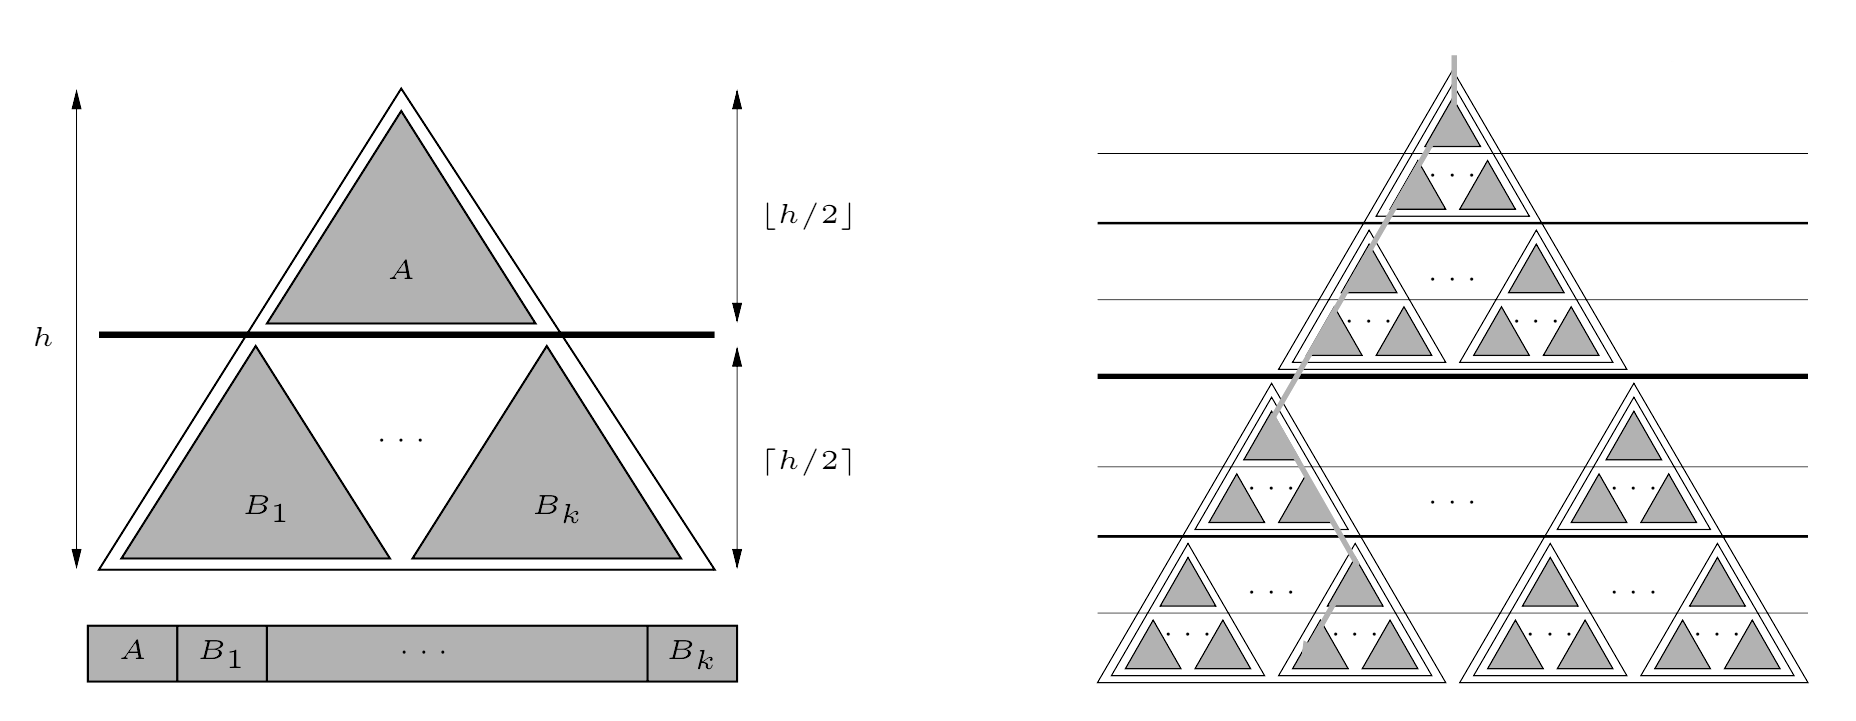
\includegraphics[]{img/vanemdeboas.png}
\end{figure}
	
\end{itemize}

\subsubsection{Dynamické cache-oblivious datové struktury}
\paragraph{Dynamické stromy}
Základní myšlenka je doplnit dynamický strom $T$ \uv{prázdnými} uzly na statický kompletní strom $T'$ a ten poté uložit v poli pomocí van Emde Boasova rozložení. Strom vyvažujeme. Pro každý uzel definujeme \textit{hustotu} $\rho(u) = \frac{|T_u|}{T'_u}$, tj. poměr reálných a (reálných + virtuálních) uzlů v podstromu zakořeněném v $u$. Pro každou úroveň definujeme horní a dolní práh hustoty uzlů na této úrovni a při porušení vyvažujeme.
\begin{figure}[H]
	\centering
	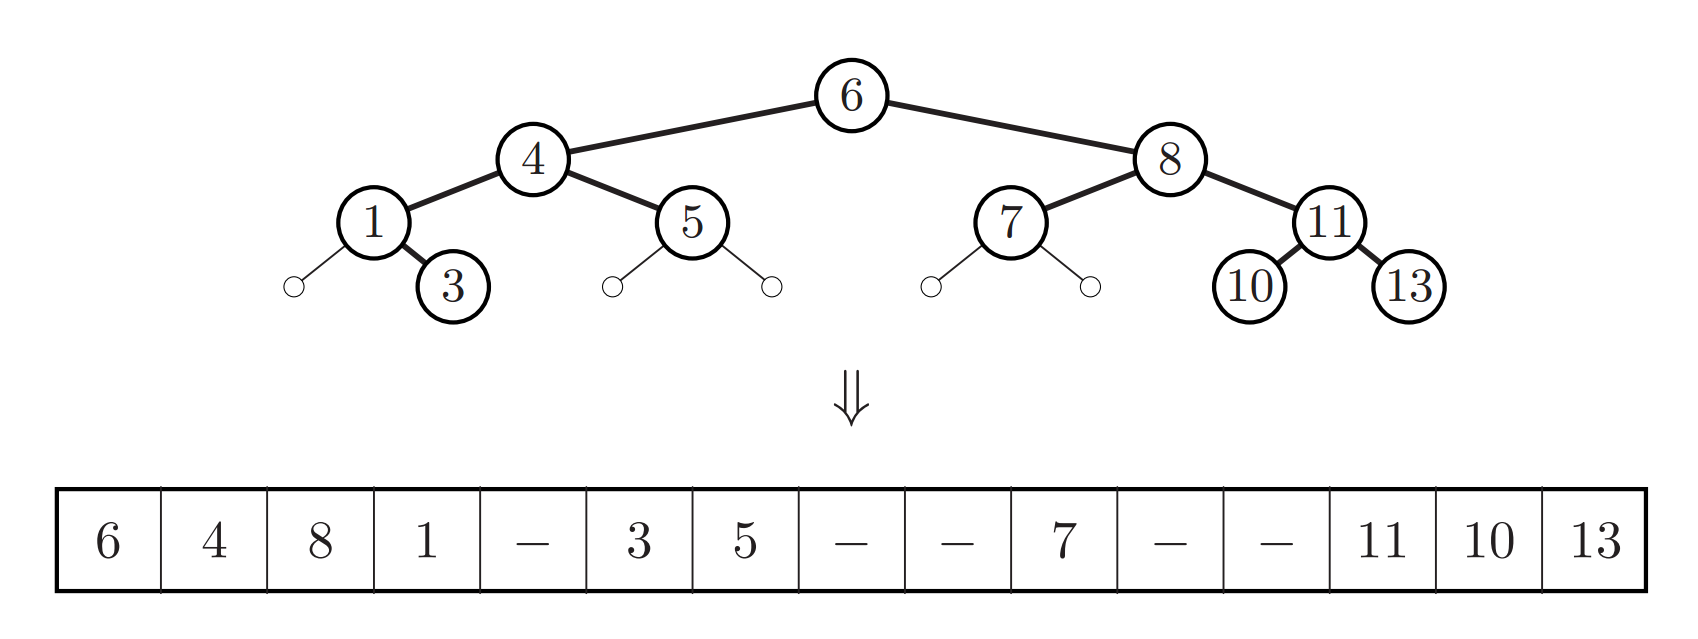
\includegraphics[width=0.8\textwidth]{img/dynamic_oblivious.png}
\end{figure}

Vyhledávání: $O(\log_B N)$, range query: $O(\log_B N + 	\frac{K}{B})$, update $O(\log_B N + \frac{\log^2N}{B})$.


\subsection{Strategie pro správu cache}
\begin{description}
	\item[OPT:] Optimální off-line algoritmus předpokladající znalost všech přístupů do paměti
	\item[FIFO:] Z cache smažeme stránku, která je ze všech stránek v cache nejdelší dobu
	\item[LRU:] Z cache smažeme stránku, která je ze všech stránek v cache nejdéle nepoužitá
\end{description}

Srovnání LRU a OPT:
\begin{theorem}[Sleator, Tarjan]
Nechť $s_1, s_2, \dots s_k$ je posloupnost přístupů do paměti, nechť LRU má k dispozici $n_{LRU}$ bloků v cache, OPT má k dispozici $n_{OPT}$ bloků v cache a $n_{LRU} > n_{OPT}$. Označme $F_{LRU}$ a $F_{OPT}$ počet přenesených bloků jednotlivých strategií (= počet výpadků cache). Pak
$$F_{LRU} \leq \frac{n_{LRU}}{n_{LRU} - n_{OPT}}\cdot F_{OPT} + n_{OPT}$$
\end{theorem}
\begin{implication}
Pokud LRU může uložit dvojnásobný počet bloků než OPT, pak má LRU nejvýše dvojnásobný počet přenesených bloků oproti OPT (plus $n_{OPT}$).
\end{implication}
Zdvojnásobení velikosti cache většinou nemá vliv na asymptotický počet přenesených bloků, viz např.:
\begin{itemize}
	\item průchod polem: $O(\frac{n}{B})$
	\item Mergesort: $O(\frac{n}{B}\log (\frac{n}{M})$
	\item Funnelsort: $O(\frac{n}{B}\log_{\frac{M}{B}} (\frac{n}{B})$
	\item van Emde Boas: $O(\log_B n)$
\end{itemize}

\begin{proof}
Rozsekáme $s_1, s_2, \dots, s_k$ na kusy, kde v každém kusu až na poslední přenese LRU přesně $n_{LRU}$ bloků (tj. dojde k $n_{LRU}$ výpadkům). To znamená, že v každém kusu se přistupuje aspoň k $n_{LRU}$ \textit{různým} blokům (plyne z definice LRU). OPT má v daném kusu nejméně $(n_{LRU} - n_{OPT})$ výpadků, neboť i při sebelepším managementu má k dispozici pouze $n_{OPT}$ bloků v cache, tedy k výpadkům nutně musí dojít.

Označíme $F'_{LRU}$ resp. $F'_{OPT}$ počet výpadků pro LRU resp. OPT v daném kusu. Platí $F'_{LRU} = n_{LRU}$ a $F'_{OPT} \geq (n_{LRU} - n_{OPT})$ a tedy
$$\frac{F'_{LRU}}{F'_{OPT}} \leq \frac{n_{LRU}}{n_{LRU} - n_{OPT}}$$

$$F'_{LRU} \leq \frac{n_{LRU}}{n_{LRU} - n_{OPT}} F'_{OPT}$$

V posledním kusu dat tato nerovnost neplatí, neboť počet výpadků LRU může být menší než $n_{LRU}$. Označme $F''_{LRU}$ resp. $F''_{OPT}$ počet výpadků pro LRU resp. OPT v posledním kusu. Stejnou logikou jako v obecném případě můžeme odvodit, že $F''_{OPT} \geq F''_{LRU} - n_{OPT}$, a tedy jednoduchou úpravou  
$$F''_{LRU} \leq F''_{OPT} + n_{OPT}$$
Díky $n_{LRU} > n_{OPT}$ také platí $\frac{n_{LRU}}{n_{LRU} - n_{OPT}} > 1$ a tedy
$$F''_{LRU} \leq \frac{n_{LRU}}{n_{LRU} - n_{OPT}}F''_{OPT} + n_{OPT}$$
\end{proof}



\part{Inteligentní agenti}

\chapter{Přírodou inspirované počítání}
\section{Genetické algoritmy, genetické a evoluční programování.}
\subsection{Evoluční algoritmy}
\textbf{Evoluční algoritmy (EA)} je souhrnné označení pro všechny výpočetní metody inspirované evolucí. Historicky se nejdříve paralelně vyvíjely 3 metodiky: genetické algoritmy, evoluční strategie a evoluční programování. Až později došlo k jejich seskupení pod společný zastřešující název: evoluční algoritmy (někdy také evoluční počítání).

EA jsou populační stochastické prohledávací algoritmy. Obecně se hodí spíše označení meta-algoritmus, jelikož pro specifické problémy se vytváří doménově specifické varianty EA s doménově danou reprezentací a vlastními implementacemi evolučních operátorů. Obecně platí \uv{no free lunch theorem} -- tj. neexistuje jeden ultimátní nejlepší algoritmus pro všechny typy problémů.

Základní struktura obecného EA je následující:
\begin{enumerate}
	\leftskip 40pt
	\setlength{\itemsep}{0pt}
	\item vytvoř náhodnou iniciální populaci $P(t=0)$, ohodnoť $P(0)$
	\item dokud není splněna ukončovací podmínka:
	\begin{enumerate}
		\leftskip 40pt
		\setlength{\itemsep}{0pt}
		\item rodičovská selekce podle fitness
		\item křížení s pravděpodobností $p_c$
		\item mutace s pravděpodobností $p_m$
		\item ohodnocení nové populace, environmentální selekce do $P(t+1)$
	\end{enumerate}
\end{enumerate}
\begin{figure}[H]
	\centering
	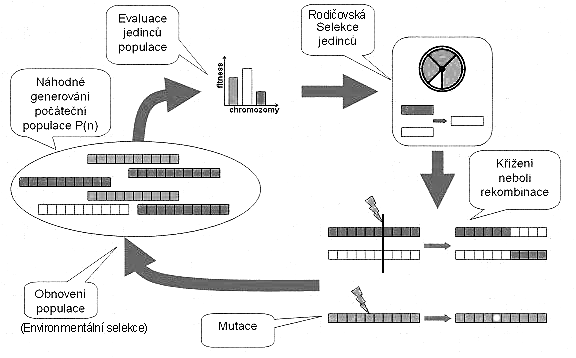
\includegraphics[width=0.8\textwidth]{img/ea.png}
\end{figure}

\subsection{Genetické algoritmy (GA)}
Původní Hollandův GA (dnes označován jako Simple GA, SGA) je nejstarší a nejjednodušší varianta EA, jejímž klíčovým rysem je to, že jedinci jsou \textbf{binární řetězce}. Používá ruletovou selekci (rodičovskou, environmentální se nepoužívá), 1-bodové křížení, bitové mutace (viz níže). V původním Hollandově návrhu je i operátor \textit{inverze}, který obrátí část řetězce, ovšem se zachováním významu bitů. Inverze se ukázala být nevýhodnou.


%TODO GA

\subsection{Genetické programování (GP)}
\begin{wrapfigure}{r}{0.3\textwidth}
\centering
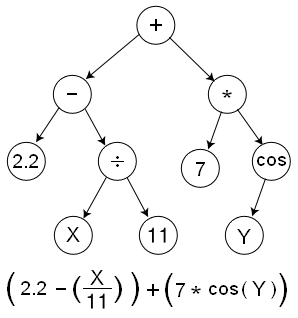
\includegraphics[width=0.25\textwidth]{img/gp.png}
\end{wrapfigure}
Tento pojem označuje genetické algoritmy, v nichž je jedincem v populaci počítačový \textbf{program}. Myšlenkou tedy je, že budeme evolvovat počítačový kód, který za nás bude řešit problémy. Duchovním otcem GP je John Koza. V jeho původní práci jsou programy reprezentovány jako syntaktické stromy, kde listy jsou proměnné a konstanty, vnitřní uzly jsou operace. \textbf{Křížení} je výměna podstromu, \textbf{mutací} se používá několik typů: mutace konstant, výměna uzlu stejné arity, permutace podstromů, záměna neterminálu za terminál apod. \textbf{Fitness} je poměrně jednoduchá: spustit vygenerovaný program na testovacích datech a ohodnotit, nakolik řeší daný problém.

Vylepšení základního principu je použití \textbf{automaticky definovaných funkcí (ADF)}. To jsou samostatné stromy, které mají omezenou množinu terminálů i neterminálů a jsou charakterizovány svou aritou. Volání nějaké ADF je pak novým terminálem, který se může vyskytnout v listech. Celý program pak sestává z hlavního stromu a několika vedlejších stromů ADF. Genetické operace GP pracují buď jen v rámci hlavního programu nebo v rámci ADF.

GP se často potýká s problémem bobtnání (\textbf{bloat}), tj. programy mají tendenci narůstat. V praxi se to řeší restrikcí velikosti či hloubky stromu, a to buď jako penalizující člen ve fitness a nebo jako kontrola (a případná eliminace) nově vznikajících jedinců. Zavádí se taky \textit{anti-bloat} operátory, tedy křížení a mutace, které jedince nezvětšují, případně jej rovnou zmenšují.

Kromě stromů lze použít i jiné struktury. \uv{Cestou dolů} jsou \textbf{lineární GP}, tj. program je lineární sekvence příkazů. To vede k jednodušším operátorům i celkové reprezentaci, rovněž rychlejší emulaci běhu; nicméně je tu velké riziko toho, že vznikne nesmyslný program. \uv{Cestou nahoru} jsou \textbf{grafové GP}, kde program je (často acyklický) graf. Vznikly nejprve jako rozšíření na paralelní programy, později získaly obecnější tvar a dnes se používají např. pro evoluci obvodů či neuronových sítí. Kvůli větší komplexitě reprezentace jsou komplikovanější i genetické operátory.

\subsection{Evoluční programování (EP)}
Evoluční programování je jeden z nejstarších směrů vývoje evolučních algoritmů, dokonce ještě o něco starší než Hollandovy GA (60. léta). Průkopníkem je Lawrence Fogel. Zásadní myšlenkou je vyvinout \uv{umělou inteligence}, konkrétně agenta, který bude umět předpovídat stav prostředí -- jinými slovy bude umět odvodit patřičnou akci v reakci na prostředí, v němž se nachází. Agent je zde reprezentován \textbf{konečným automatem}, prostředí je pak \textbf{sekvence symbolů konečné abecedy}.

Samotná evoluce pak vypadá takto: jedinci v populaci jsou konečné automaty, těm jsou předkládány vstupy. Jejich výstup je vždy porovnán s následujícím vstupem v posloupnosti. Fitness je úspěšnost predikce, přičemž se může měřit různě: vše nebo nic, absolutní chyba, mean square error. Často je do fitness započítána i velikost automatu.

\textit{Každý} automat podstoupí mutaci, která může mít různou \uv{intenzitu} -- od malých, \uv{kosmetických} změn po radikální. Příklady mutací jsou: změna výstupního symbolu, změna následného stavu, přidání stavu, odebrání stavu, změna počátečního stavu, \dots Noví jedinci jsou ohodnoceni a poté je vybráno (z nových i starých najednou) $N$ jedinců do nové populace. Výběr probíhá buď turnajem, nebo deterministicky (tj. vezme se $N$ nejlepších jedinců. (Pozn.: V původním algoritmu není nijak omezeno, kolik potomků může být vygenerováno z jednoho rodiče, ani že velikost populace musí zůstávat konstantní.)

\textbf{Křížení neexistuje (!)}. 

V dnešní době se EP vyvinulo do obecnější podoby. Zakódování jedinců je velmi benevolentní a mělo by být přirozené pro daný problém (často genotyp = fenotyp). Používá se více \uv{chytrých mutací}, které jsou těsně přizpůsobeny problému a dané reprezentaci. Křížení se typicky nepoužívá. Rodičovská selekce je prostá: každý jedinec se vybere právě jednou. Environmentální selekce je turnajová na spojené populaci rodičů a potomků.

Jelikož se EP vyvíjelo paralelně s GA i ES, jsou mezi nimi nevyhnutelně mnohé podobnosti. Pojďme si tyto metody porovnat.

\subsubsection{EP vs. GA}
V GA jsou jedinci sekvence symbolů abecedy, původně pouze binární, dnes už vcelku libovolné. V EP není žádné omezení na podobu reprezentace a typicky je přizpůsobena problému (jedinec může být např. neuronová síť). 

Mutace funguje rovněž trochu jinak. V EP máme škálu mutací od malých změn až po radikální zásahy, přičemž pravděpodobnost aplikace mutace je nepřímo úměrná její závažnosti. Celková závažnost mutací se rovněž může snižovat v průběhu konvergence k optimálnímu řešení.

Zjevným rozdílem je rovněž absence křížení u EP.

\subsubsection{EP vs. ES}
Pokud je jedincem v EP posloupnost reálných čísel, začínají být velice podobné evolučním strategiím. EP dokonce také mohou být \textit{self-adaptive}, tj. jedinec nese kromě genotypu i parametry ovlivňující evoluci, konkrétně míru závažnosti mutací (rozptyl gaussovské mutace).

Existují však rozdíly: EP používá turnajovou selekci, ES deterministicky odstraňuje dané množství nejhorších řešení. Druhým rozdílem je absence křížení u EP, zatímco ES je často implementuje. 

\subsubsection{Význam křížení}
Malá odbočka: trpí EP tím, že nemá křížení? Pomáhá vlastně křížení, nebo stačí mutace? Jones (1995) provedl tzv. \uv{headless chicken epxeriment}: porovnával klasické GA a GA, kde je klasické křížení nahrazeno \uv{náhodným křížením}. To funguje tak, že se dva vybraní jedinci nezkříží mezi sebou, namísto toho se pro každého z nich vygeneruje partner jako náhodná sekvence z domény (tj. například náhodný binární vektor správné délky). Pak se provede jednobodové křížení a od každého rodiče se vybere jeden potomek. Jones označil tento operátor jako \textit{headless chicken} -- stejně jako bezhlavé kuře pobíhající po dvorku není doopravdy kuře (protože mu něco důležitého chybí), tak ani toto \uv{náhodné křížení} není vlastně křížení, protože při něm vůbec nedochází ke kontaktu mezi jedinci. Jedná se ve skutečnosti o jakousi makromutaci.

Pointou experimentu bylo porovnat výkonnost obou variant a určit, nakolik opravdové křížení skutečně pomáhá. Závěrem bylo konstatování, že pokud má problém jasně definované stavební bloky, pak křížení skutečně pomáhá (především na začátku evoluce), zatímco pokud nejsou bloky zřejmé, pak křížení příliš nepomáhá (výkon obou variant byl srovnatelný).

\section{Teorie schémat, pravděpodobnostní modely jednoduchého genetického algoritmu.}
\subsection{Schémata}
\textbf{Schéma} v kontextu genetických algoritmů (tj. jedinec je slovo v abecedě \{0,1\}) je reprezentace množiny jedinců jako slova v abecedě \{0,1,*\}, kde * označuje libovolný symbol (\uv{žolík}). Například schéma 0*11* reprezentuje množinu jedinců \{00110, 00111, 01110, 01111\}. Platí následující:
\begin{itemize}
	\leftskip 20pt
	\setlength{\itemsep}{0pt}
	\item schéma s $r$ * reprezentuje $2^r$ jedinců
	\item jedinec délky $m$ je reprezentován $2^m$ schématy
	\item je $3^m$ schémat délky $m$
	\item v populaci velikosti $n$ je $2^m$ až $n\cdot2^m$ schémat
\end{itemize}
Pro schéma S lze definovat následující vlastnosti:
\begin{description}
	\leftskip 20pt
	\setlength{\itemsep}{0pt}
	\item[Řád schématu o(S):] počet pevných pozic (0 a 1) 
	\item[Definující délka d(S):] vzdálenost mezi první a poslední pevnou pozicí
	\item[Fitness F(S)] průměrná fitness odpovídajících jedinců v populaci
\end{description}

\noindent\textbf{Věta o schématech (VoS):} \textit{Krátká schémata s nadprůměrnou fitness a malým řádem se v populaci během GA exponenciálně množí.}


\begin{proof} Budeme zkoumat, co se děje s konkrétním schématem $S$ během selekce, křížení a mutace.

Nechť $P(t)$ je populace v čase $t$, $n$ je velikost populace, $m$ je délka jedinců v populaci, $C(S,t)$ je četnost schématu $S$ v populaci $P(t)$ (tj. počet jedinců v $P(t)$ reprezentovaných $S$). Budeme odhadovat $P(S, t+1)$.

\textit{Selekce:} Schéma $S$ má pravděpodobnost vybrání
$$p_s(S) = \frac{F(S)}{\sum\limits_{u \in P(t)}F(u)}$$
Tedy 
$$C(S,t+1) = C(S,t) \cdot n \cdot p_s(S)$$
neboť provádím $n$ výběrů do nové populace pomocí ruletové selekce, přičemž na ruletě zabírají jedinci odpovídající schématu $S$ právě $C(S,t) \cdot p_s(S)$ procent místa. Ekvivalentně lze psát
$$C(S,t+1) = C(S,t) \cdot \frac{F(S)}{\frac{\sum_{u \in P(t)}F(u)}{n}} = C(S,t) \cdot \frac{F(S)}{F_{avg}(t)}$$
kde $F_avg(t)$ označuje průměrnou fitness v populaci $P(t)$. 

Představme si, že schéma $S$ je nadprůměrné o $\varepsilon$\,\%, tj. $F(S) = F_{avg}(t) + \varepsilon\cdot F_{avg}(t)$. Pak 
$$C(S,t+1) = C(S,t)(1+\varepsilon)$$
$$C(S,t+1) = C(S,0)(1+\varepsilon)^t$$
Tedy četnost nadprůměrných schémat roste geometrickou řadou.

\textit{Křížení:} Předpokládáme klasické jednobodové křížení. Pravděpodobnost, že schéma $S$ křížení nepřežije, je 
$$p_{death}(S) = \frac{d(S)}{m-1}$$
a tedy pravděpodobnost přežití je 
$$p_{surv}(S) \geq 1 - p_c \cdot \frac{d(S)}{m-1}$$
kde $p_c$ je pravděpodobnost křížení. Všimněte si nerovnosti: je totiž šance, že i když se bod křížení \uv{trefí} dovnitř schématu, tak část doplněná s druhého rodiče bude pořád odpovídat schématu a celkově tedy schéma přežije. Zjevné je to například při křížení dvou totožných jedinců (tam schéma přežije vždy).

\textit{Mutace:} Pravděpodobnost změny jednoho bitu je $p_m$, pravděpodobnost přežití schématu je tedy 
$$p_{surv}(S) = (1-p_m)^{o(S)}$$
$$p_{surv}(S) \approx 1 - p_m \cdot o(S)$$
Poslední aproximace funguje pro $p_m \ll 1$.

Dohromady tedy dostáváme:
$$C(S,t+1) \geq C(S,t) \cdot \frac{F(S)}{F_{avg}(t)} \cdot \left(1 - p_c \cdot \frac{d(S)}{m-1} - p_m \cdot o(S)\right)$$
\end{proof}

\textbf{Hypotéza o stavebních blocích (HoSB)} GA hledá suboptimální řešení problému rekombinací krátkých, nadprůměrných s malým řádem schémat (\uv{building blocks}).

\subsubsection{Důsledky VoS}
GA pracuje s $n$ jedinci, ale implicitně vyvíjí mnohem více schémat: $2^m$ až $n\,2^m$ (implicitní paralelismus). Holland tvrdí, že za splnění jistých předpokladů ($n = 2^m$, schémata zůstávají nadprůměrná, \dots) platí, že počet schémat, kterým se v GA dostává exponenciálního růstu je úměrný $n^3$. 

GA také optimálně řeší problém explorace a exploatace, což lze ukázat na analogii s tzv. \textbf{2-rukým banditou}: \textit{Mám N mincí, ruce bandity (= hrací automat) vyplácí se střední hodnotou $m_1$ resp. $m_2$ a rozptylem $s_1$ resp. $s_2$, cílem je maximalizovat zisk. Analytickým řešením je alokovat exponenciálně více pokusů pro právě vyhrávající ruku.} GA rovněž alokuje exponenciálně mnoho nadějným schématům. Nejdříve se myslelo, že GA hraje $3^m$-rukého banditu, tj. všechna schémata jsou konkurenční ruce. Ve skutečnosti se hraje více her, v nichž schémata soutěží o konfliktní pevné pozice: schémata řádu $k$ soutěží právě o těch $k$ pozic -- hrají spolu $2^k$-rukého banditu. To stále není úplně přesné, protože na rozdíl od bandity, kde jsou ruce nezávislé, nesampluje GA schémata nezávisle.

Problémem také je, že GA často neodhadne správně skutečnou fitness schémat. Např. je-li F(111*\dots*)~= 2, F(0*\dots*) = 1 a jinak F(x) = 0, pak platí F(1*\dots*) = $\frac{1}{2}$, F(0*\dots*) = 1. Jenže GA odhadne F(1*\dots*) $\approx$ 2, protože 111*\dots* v populaci převáží. Tomuto se říká \textit{kolaterální konverence}, tj. jakmile se někam začne konvergovat, už nejsou schémata samplována rovnoměrně a fitness se neodhadne správně. Podobným problémem je velký rozptyl fitness (např. 1*\dots* z předchozího příkladu). GA bude nejspíše konvergovat tam, kde je fitness větší $\rightarrow$ chybný odhad statické fitness.


\subsection{Pravděpodobnostní modely}
Od 90. let se objevují snahy přesně modelovat chování GA, konkrétně: jak přesně vypadají populace, zobrazení přechodu k další populaci, vlastnosti tohoto zobrazení, asymptotické chování jednoduchého GA. Existují modely pro konečné i nekonečné populace.

\subsubsection{Ještě jednodušší jednoduchý GA (JJJGA)}
Pro jednodušší tvorbu modelů byl původní jednoduchý GA ještě o něco zjednodušen a formalizován takto:
\begin{itemize}
	\leftskip 20pt
	\setlength{\itemsep}{0pt}
	\item inicializuj náhodnou počáteční populaci binárních řetězců $x$ délky $l$
	\item dokud nenajdeš dost dobré $x$:
	\begin{itemize}
		\leftskip 40pt
		\setlength{\itemsep}{0pt}
		\item dokud nenaplníš novou populaci:
		\begin{itemize}
			\leftskip 40pt
			\setlength{\itemsep}{0pt}
			\item vyber selekcí 2 jedince, zkřiž je s pravděpodobností $p_c$, jednoho potomka zahoď
			\item mutuj každý bit nového řetězce s pravděpodobností $p_m$
			\item vlož do nové populace
		\end{itemize}
	\end{itemize}
\end{itemize}

\subsubsection{Analýza}
Každý jedinec je tedy binární řetězec délky $l$, což lze chápat jako binární zápis nějakého čísla [0, \dots, $2^l-1$] (např. 00000111 je 7). Populace v čase $t$ je reprezentována dvěma vektory $p(t)$ a $s(t)$, oba délky $2^l$. Číslo $p_i(t)$ vyjadřuje, kolik procent populace zabírá řetězec $i$; číslo $s_i(t)$ vyjadřuje pravděpodobnost selekce řetězce $i$.

Dále definujeme matici $F$ takto: $F(i,i) = f(i); F(i,j) = 0$ pro $i \neq j$. Hodnota $f(i)$ je fitness jedince $i$. Pak můžeme definovat vztah vektorů $s(t)$ a $p(t)$ jako
$$s(t) = \frac{F \cdot p(t)}{\sum\limits_{j=0}^{2^l-1} F(j,j) \cdot p_j(t)}$$

Naším ideálem je definovat matici G, která realizuje jeden krok JJGA, tj. $p(t+1) = G \cdot p(t)$, nebo obdobně $s(t+1) = G \cdot s(t)$. Toto zobrazení bude fungovat jako složení dvou dílčích zobrazení: matice F (fitness) a matice M (mutace a křížení). 

Nejprve uvažme $G=F$ (tj. nemáme žádné genetické operátory). Platí $E(p(t+1)) = s(t)$, kde $E$ je střední hodnota. Pak díky $s(t+1) \sim F \cdot p(t+1)$ (liší se jen o multiplikativní odchylku) můžeme psát $E(s(t+1)) \sim F \cdot s(t)$. V případě konečné populace nám výběrové chyby mohou způsobit odchylku od $E()$, obecně čím větší populace, tím menší odchylka. U nekonečné populace by to bylo přesné.

Nyní se podívejme na situaci $G = M$, tedy neřešíme selekci. Zde využijeme pomocnou veličinu $r(i,j,k)$, která udává pravděpodobnost, že z $i$ a $j$ vznikne $k$. Když tuto veličinu známe, pak lze vyjádřit 
$$E(p_k(t+1)) = \sum\limits_{i=0}^{2^l-1} \sum\limits_{j=0}^{2^l-1} s_i(t) \cdot s_j(t) \cdot r(i,j,k)$$
Funkci $r(i,j,k)$ lze analyticky spočíst.\footnote{\url{http://ktiml.mff.cuni.cz/~neruda/eva2-13.pdf}}

Závěr: JJGA pracující prostřednictvím $G$ je dynamický systém, $p(t)$ či $s(t)$ jsou body (trajektorie). Neznáme jeho pevné body, můžeme však vyjádřit pevné body jednotlivých zobrazení: Pevné body F jsou populace se stejnou fitness, stabilní pevný bod F je maximální stejná fitness. (Jediný) pevný bod M: stejné pravděpodobnosti $s$ (resp. stejné zastoupení jedinců $p$). Kombinace míchání M a ostření F odpovídá fenoménu \textit{punctuated equilibria} (známe z biologie).

\subsubsection{Konečné populace}
Pro konečné populace lze definovat GA jako \textit{markovovský řetězec}, tj. stochastický proces v systému se stavy a přechody mezi stavy s definovanými pravděpodobnostmi. Pravděpodobnost přechodu závisí vždy pouze na předchozím stavu. Jeden stav systému je jedna konkrétní populace. Populací o $n$ jedincích délky $l$ je $N = \binom{n+2^l-1}{2^l-1}$, matice pravděpodobností přechodů je $N\times N$, podrobnější rozbor opět v Nerudových slajdech.

Dokázala se korespondence ideálního JJGA s nekonečnou populací a modelu s konečnou populací (pro $n \rightarrow \infty$).






\section{Evoluční strategie, diferenciální evoluce, koevoluce, otevřená evoluce.} 
\subsection{Evoluční strategie}
\textbf{Evoluční strategie (ES)} je metoda pro optimalizaci reálných funkcí, která je výjimečná tím, že jako první používala \textit{self-adaptation}, tj. parametry evoluce byly součástí jedince -- šlo tedy o \uv{evoluci evoluce}. Evolvovaný jedinec se tedy skládá z \textbf{genetických parametrů} ovlivňujících chování a \textbf{strategických parametrů} ovlivňující evoluci.

Vznikly v 60. letech, autoři \textbf{Rechenberg a Schwefel.} ES jsou jedna z větví evolučních algoritmů (anglicky se jako \uv{umbrella term} používá buď \textit{Evolutionary Algorithms} nebo \textit{Evolutionary Computation}), nicméně nevyčlenily se v průběhu, jak by se dalo čekat. ES se vyvíjely paralelně s GA a EP (evolučním programováním), až později došlo k seskupení těchto tří metod pod jeden společný obor.

\subsubsection{Notace}
\begin{description}
	\leftskip 20pt
	\setlength{\itemsep}{0pt}
	\item[\textit{M}] počet jedinců v populaci
	\item[\textit{L}] počet vznikajících potomků
	\item[\textit{R}] počet rodičů každého nového jedince
\end{description}
Doporučení: $M > 1$, $L > M$ aby se vytvořily různé selekce (např. $L \approx 7 \cdot M$)

\subsubsection{Varianty}
\begin{description}
	\leftskip 20pt
	\setlength{\itemsep}{0pt}
	\item[\textit{(M+L)} ES] -- M jedinců do nové populace je vybráno z M+L starých i nových jedinců
	\item[\textit{(M,L)} ES] -- M nových jedinců je vybráno jen z L nových potomků (tato varianta se ukázala být robustnější vůči uvíznutí v lokálních extrémech)
\end{description}

\subsubsection{Kódování, genetické operátory}
Jedinec je tvaru $C(i) = [G_n(i), S_k(i)], k \in \{1, n, 2n\}$, tedy první část je samotný genotyp, druhá část jsou parametry evoluce, konkrétně \textbf{hodnoty standardních odchylek floating point mutací}. Podle hodnoty $k$ rozlišujeme 3 varianty:
\begin{description}
	\leftskip 20pt
	\setlength{\itemsep}{0pt}
	\item[k=1]: jedna společná odchylka pro všechny parametry
	\item[k=n]: nekorelované mutace; geometricky se mutuje po elipse rovnoběžné s osami
	\item[k=2n]: korelované mutace, odpovídají mutování z n-rozměrného normálního rozdělení. 
	Pro uložení korelační matice stačí n-rozměrný vektor (???). Tato matice odpovídá matici rotace (tj. elipsa se natočí v optimálním směru).
\end{description}

\begin{figure}[h]
	\centering
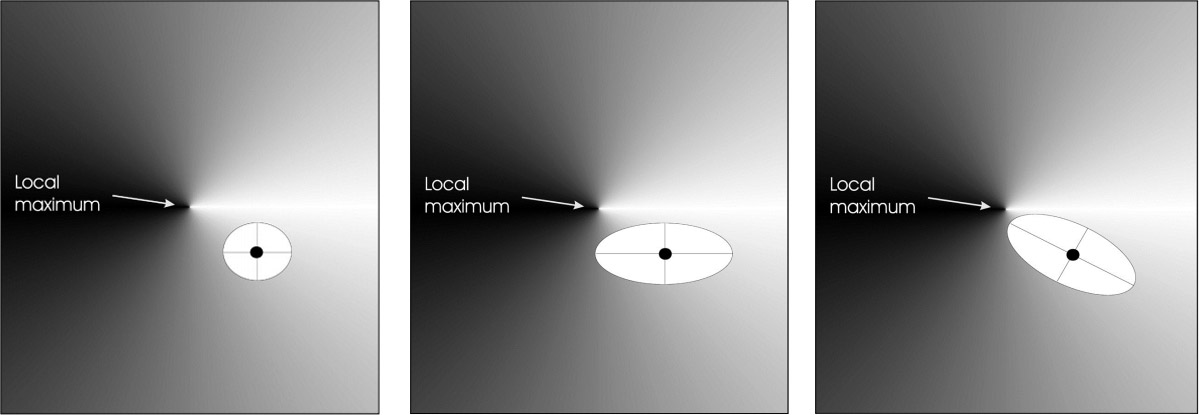
\includegraphics[width=0.7\textwidth]{img/ES_varianty_k.jpg}
\end{figure}

\textbf{Populační cyklus} vypadá takto:
\medskip

\begin{minipage}{\linewidth}
	\begin{lstlisting}[frame=single]
n=0, randomly init population P[n] of size M
evaluate fitness of individuals in P[n]
while not good enough:
	repeat L times:
		choose R parents
		crossover, mutate, evaluate new individual
	choose M new individuals (by the type of ES)
	n++
	\end{lstlisting}
\end{minipage}

Nový jedinec je akceptován pouze tehdy, je-li lepší než rodič -- pak rodiče nahradí.

\textbf{Mutace} jedince probíhá takto: \textit{genetické} parametry (genotyp) jsou změněny přičtením náhodného čísla s norm. rozdělení s příslušnou odchylkou (a případně i rotací). \textit{Strategické} parametry = odchylky jsou zvětšeny nebo zmenšeny podle \uv{pravidla $1/5$}, což heuristika, která říká, že nejlepší je, když má mutace úspěšnost 20\,\% (tzn. při menší zvyš odchylku, při větší sniž). V případě varianty s rotacemi jsou mezi strategickými parametry také hodnoty rotací -- ty se mutují jednoduše přičtením náhodného čísla z N(0,1).

\textbf{Křížení} je uniformní, typicky více rodičů. Podle velikosti R mluvíme o lokálním (R=2) nebo globálním (R=M). Může být diskrétní (použij hodnotu náhodně vybraného rodiče) nebo aritmetické (průměr).

\subsubsection{CMA-ES}
Dnes nejkomplexnější verzí je \textbf{CMA-ES} (Correlation Matrix Adaptation ES). Udržuje se korelační matice proměnných, která se inkrementálně aktualizuje po každém kroku metodou maximum-likelihood.

\subsection{Diferenciální evoluce}
Alternativní algoritmus spojité optimalizace, který funguje dobře i pro funkce které jsou nediferencovatelné, nespojité, zašuměné, neseparabilní nebo vysoce podmíněné. Každý jedinec prochází opakovaně cyklem \textbf{mutace} $\rightarrow$ \textbf{křížení} $\rightarrow$ \textbf{selekce}. Během mutace dochází k posunu \uv{podle ostatních}, tj. jedinec se posouvá ve směru populace. DE je také invariantní vůči rotaci či škálování prohledávaného prostoru.
\begin{figure}[H]
	\centering
	\includegraphics[width=0.7\textwidth]{img/DE_scheme.png}
\end{figure}

\subsubsection{Mutace}
V populaci $p$ zvolíme pro jedince $x_{i,p}$ tři různé jedince: $x_{a,p}$, $x_{b,p}$ a $x_{c,p}$. Definujeme donora: $$v_{i,p+1} = x_{a,p} + F \cdot (x_{b,p} - x_{c,p})$$ kde $F \in \langle 0; 2 \rangle$ je parametr mutace.
\subsubsection{Křížení}
Uniformní křížení původního jedince s donorem. Parametr $C$ určuje pravděpodobnost změny, $rand_{ij} \in \langle0,1\rangle$ je pseudonáhodné číslo. Číslo $I_{rand}$ je náhodný index z $\langle 1,2,...D\rangle$, kde $D$ je délka jedince. Pak vytvoříme pokusný vektor $u_{i,p+1}$ jako:
$$u_{i,p+1}[j] = v_{i,p+1}[j] \leftrightarrow rand_{ji} \leq C \lor j = I_{rand}$$
$$u_{i,p+1}[j] = x_{i,p}[j] \leftrightarrow rand_{ji} > C \land j \neq I_{rand}$$

Díky $I_{rand}$ je zajištěno, že ve výsledku bude aspoň jeden prvek z donora.

\subsubsection{Selekce}
Jako nový jedinec $x_{i,p+1}$ se vezme lepší (dle fitness) z dvojice $x_{i,p}$, $u_{i,p+1}$.

\subsection{Koevoluce}
Situace, kdy se dva či více druhů vyvíjí závisle na sobě, tj. fitness jedince není závislá pouze na prostředí, ale především na interakci s jinými jedinci (tzv. \textit{kontextová fitness}). Rozlišujeme koevoluci \textbf{kooperativní} a \textbf{kompetitivní}. Typickým modelem kompetitivní koevoluce je tzv. \textbf{dravec-kořist} (predator-prey). Kompetitivně lze rovněž vyvíjet strategie pro nejrůznější hry - např. dáma apod.

%TODO koevoluce

\subsection{Otevřená evoluce}
Evoluce bez konce, tj. neexistuje ukončovací podmínka ani optimální řešení, neboť fitness funkce je \textit{dynamická}. Často je dynamické i kódování jedince -- např. pokud u neuroevoluce mohou síti ubývat a přibývat neurony či synapse. 

Míra změn fitness může být různá: 
\begin{description}
	\leftskip 30pt
	\setlength{\itemsep}{0pt}
	\item[malé změny] robot se opotřebuje, v chemické továrně se trochu změní suroviny apod.
	\item[výrazné morfologické změny] vrcholy zanikají, nové vznikají, \uv{emerging markets}
	\item[cyklické změny] roční období, spotřeba elektřiny, \dots
	\item[katastrofické změny] bouchla elektrárna, nehoda na dálnici, \dots
\end{description}

Byly navrženy různé postupy pro vyrovnání se s dynamickou fitness. Například \textit{vyvolaná hypermutace} (při snížení fitness), \textit{náhodná migrace} (při snížení fitness se generují noví náhodní jedinci) a obecně metody vedoucí k udržení diverzity populace: zmenšení selekčního tlaku, crowding, niching, subpopulace, dynamické druhy (které se množí jen mezi sebou).

Dynamická fitness je vyvolaná i kompetitivní koevolucí, a tedy evoluční souboje typ lovec-kořist lze označit za otevřenou evoluci.


%TODO otevřená evoluce


\section{Rojové optimalizační algoritmy.}
\subsection{Optimalizace hejnem částic}
Anglicky \textit{particle swarm optimization} -- jedná se o populační prohledávací algoritmus inspirovaný hejny ptáků/hmyzu/ryb. Jedinec se nazývá \textbf{částice} a jde typicky o vektor reálných čísel. Neexistují křížení ani mutace, jak je známe.

\subsubsection{Algorimus}
\begin{minipage}{\linewidth}
	\begin{lstlisting}[frame=single, escapeinside={\%*}{*)}]
init each particle
while not (max iterations or minimum error)
	foreach particle p:
		f = fitness(p)
		if f > p.pBest
			p.pBest = f
	gBest = max(p.pBest for each particle p)			
	foreach particle p:
		p.v = p.v + 
			+ c1 * rand(0,1) * (pBest - p.position) 
			+ c2 * rand(0,1) * (gBest - p.position) 
		p.position += p.v		
	\end{lstlisting}
\end{minipage}

Každá částice má rychlostní vektor $v$, který se aktualizuje podle nejlepší pozice částice v historii (řádek 10) a nejlepší globální pozice v historii (řádek 11). Učicí konstanty c1,c2 se často nastavují na c1 = c2 = 2. \\
\textit{Pozn. celé to asi může být v jednom for cyklu s tím, že gBest se aktualizuje průběžně a ne po "generacích".}

PSO jsou podobné GA -- stochastický model, fitness pro ohodnocení, náhodná iniciální konfigurace atd. -- ale současně se v mnohém liší: neexistují genetické operace, částice mají paměť a výměna informací probíhá pouze od nejlepších částic ostatním. 

PSO nepoužívají gradient pro optimalizaci, což znamená, že optimalizovaná funkce nemusí být diferencovatelná.


\subsection{Další rojové optimalizační algoritmy}
Obecně se definuje \textbf{Swarm Intelligence (SI)} jako \textit{“The emergent collective intelligence of groups of simple agents"}. Dvě základní vlastnosti jsou sebeorganizace a dělba práce. Kromě PSO sem lze zařadit ještě Ant Colony Optimization (ACO), Artificial Bee Colony (ABC), Glowworm Swarm Optimization, Cuckoo Search Algorithms a v jistém směru sem spadá i diferenciální evoluce (jelikož je population-based). Kromě DE se tyto algoritmy (a mnohé další, třeba i simlated annealing)  označují také nálepkou \textit{metaphor-based metaheuristics}, a to díky tomu, že jsou typicky insipirované nějakou reálnou skutečností (chování roje, chování mravenců, zpracování kovů apod.). Tyto se staly terčem kritiky pro nedostatek inovace a efektivity, kterou schovávají právě za poutavou metaforou (\url{https://en.wikipedia.org/wiki/List_of_metaphor-based_metaheuristics}).

\subsubsection{Ant Colony Optimization (ACO)}
Systém inspirovaný chování mravenců při hledání potravy, konkrétně použitím feromonů. V podstatě jde o techniku nalezení nejlepší cesty v grafu. Agent (mravenec) se pohybuje v grafu a zanechává za sebou feromonovou stopu. Pohyb se řídí rovnicí:
$$p^k_{ij}(t) = \frac{([\tau_{ij}(t)]^\alpha \cdot [\eta_{ij}]^\beta)}{(\sum\limits_{n \in J_k}[\tau_{in}(t)]^\alpha \cdot [\eta_{in}]^\beta)}$$

$p^k_{ij}(t)$ je pravděpodobnost přechodu mravence $k$ z uzlu $i$ do uzlu $j$ v čase $t$, $J_k$ jsou uzly, kam má mravenec $k$ povoleno jít, $\eta_{ij}$ symbolizuje \uv{viditelnost} mezi $i$ a $j$ a $\tau_{ij}(t)$ reprezentuje množství nevypařeného feromonu mezi $i$ a $j$ v čase $t$. Parametry $\alpha$ a $\beta$ kontrolují, nakolik prohledávání závisí na feromonech. Každý mravenec $k$ má také tabu list navštívených uzlů, aby nenavštívil nějaký dvakrát.

Umístění feromonů se řídí rovnicí:
\[
\Delta\tau^k_{ij} = 
\begin{cases}
	\frac{Q}{L_k}(t) 	& \quad \text{leží-li hrana $ij$ na cestě mravence $k$} \\
	0 					& \quad \text{jinak}\\
\end{cases}
\]

$Q$ je konstanta, $L_k$ je cena cesty (její délka), $k$ je mravenec, $t$ je čas (iterace).

Feromony se časem vypařují. Celková změna feromonu na hraně $ij$ je tedy:
$$\tau_{ij}(t+1) = (1-p)\tau_{ij}(t) + \sum_{k=1}^m [\Delta\tau^k_{ij}(t)]$$
kde $m$ je počet mravenců a $p$ je míra vypařování. To je důležitý parametr algoritmu, který ovlivňuje poměr mezi explorací a exploatací.

Mírně vylepšená varianta ACO je Ant Colony System (ACS).

Dobrý přehled dalších algoritmů (např Artificial Bee Colony) lze nalézt na \url{http://journals.plos.org/plosone/article?id=10.1371/journal.pone.0122827}






\section{Memetické algoritmy, hill climbing, simulované žíhání.}
\textbf{Memetické algoritmy} jsou EA obohacené o lokální prohledávání uvnitř cyklu. Základní princip je ten, že evolucí vyvinutý jedinec ještě před ohodnocením podstoupí proceduru lokálního prohledávání -- to může být např. hill climbing, simulované žíhání nebo backpropagation u ANN). 

Inspirováno \textbf{mémy} (angl. \textit{meme} (čti /mi:m/)), což jsou ideje/myšlenky šířící se ve společnosti, které mohou podstoupit mutaci či selekci, stejně jedinci v klasické evoluci. 

Alternativně jsou MA označovány jako \textit{Baldwinian EA}, \textit{Lamarckian EA} nebo jako \textit{genetic local search}.

\subsubsection{Algoritmus}
\begin{minipage}{\linewidth}
	\begin{lstlisting}[frame=single, escapeinside={\%*}{*)}]
t = 0, initialize P[0]
P[0].localSearch()
evaluate(P[0])
while notTerminated do
	P[t] = selectIndividuals()
	mutate(P[t])
	P[t].localSearch()
	evaluate(P[t])
	P[t+1] = buildNextGen(P[t])
	t++

	\end{lstlisting}
\end{minipage}

\subsubsection{Existují dva přístupy, co dělat s výsledkem:}
\begin{description}
	\leftskip 20pt
	\setlength{\itemsep}{0pt}
	\item[Lamarckismus] Když prohledáváním najdu lepšího jedince, vezmu ho (to je ovšem darwinisticky nekorektní, změnil jsem genotyp na základě fenotypu).
	\item[Baldwinismus] Když lokálním prohledáváním najdu lepšího jedince, vezmu jen jeho fitness (ale neměním genotyp).
\end{description}


\subsubsection{Hill climbing}
Nejjednodušší informovaná metoda lokálního prohledávání stavového prostoru. Vstupem je uzel, ze kterého se má prohledávání zahájit. Nejprve je uzel expandován - jsou vygenerovány jeho sousední uzly a tyto uzly jsou ohodnoceny. Algoritmus vybere z nich nejlépe ohodnocený uzel a ten je nadále expandován. 

Algoritmus tak expanduje uzly se stále vyšším ohodnocením, dokud nenarazí na uzel po jehož expanzi mají všechny jeho sousední uzly horší ohodnocení. Algoritmus nemá paměť, navštívené uzly okamžitě zapomíná.

\medskip\textbf{Varianty:}
\begin{description}
	\leftskip 30pt
	\setlength{\itemsep}{0pt}
	\item[first choice HC vs. steepest ascent HC] First choide HC vezme prvního lepšího souseda, steepest zkusí všechny a vezme nejlepšího.
	\item[stochastic HC] Ze zlepšujících sousedů vybere náhodně podle míry zlepšení.
	\item[random restart HC (or shotgun HC)] Náhodné restarty v různých místech, částečně řeší problém uvíznutí v lokálním optimu.
\end{description}


\subsubsection{Simulované žíhání}
	\setlength\intextsep{0pt}
\begin{wrapfigure}{r}{0.35\textwidth}
	\centering

	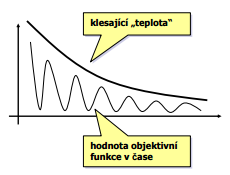
\includegraphics[width=0.3\textwidth]{img/simulated_annealing.png}
\end{wrapfigure}
Lokální prohledávání kombinující HC a náhodnou procházku. Algoritmus náhodně volí stav okolí a vydá se do něj pokud:
\begin{itemize}
	\leftskip 20pt
	\setlength{\itemsep}{0pt}
	\item je lepší než aktuální stav
	\item je horší, ale zhoršení je povoleno s určitou mírou pravděpodobnosti odvozenou od aktuální \textbf{teploty}; teplota se přitom postupně snižuje podle „ochlazovacího“ schématu
\end{itemize}


\subsubsection{Algoritmus}
\begin{minipage}{\linewidth}
\begin{lstlisting}[frame=single, escapeinside={\%*}{*)}]
	current = init()
	for t = 1 to %*$\infty$*)
		T = schedule(t)
		if T = 0 then 
			return current
		next = randomNeighbor(current)
		%*$\Delta$E*) = f(next) - f(current)
		if (%*$\Delta$E*) > 0) or (%*$e^{\Delta{}E/T} < $*) rand(0,1))
			current = next
\end{lstlisting}
\end{minipage}






\section{Aplikace evolučních algoritmů (evoluce expertních systému, neuroevoluce, řešení kombinatorických úloh, vícekriteriální optimalizace).}
\subsection{Evoluce expertních systémů}
Expertní systémy jsou modely z oblasti \textit{strojového učení}, jejichž základní charakteristikou je, že pro výpočet svého výstupu používají pravidla IF: THEN. Zastupují tedy větev strojového učení založenou na \textit{formální logice} (druhá, protikladná větev, reprezentovaná především neuronovými sítěmi, je založena na \textit{konekcionismu}, tj. modeluje biologické fungování mozku, nikoli logické). Expertní systémy, které se učí pomocí simulované evoluce, se nazývají \textbf{learning classifier systems (LCS)}. Existují dvě základní paradigmata: \textit{michiganský přístup} (jedinec je pravidlo) a \textit{pittsburghský přístup} (jedinec je množina pravidel).

\begin{wrapfigure}{r}{0.45\textwidth}
\centering
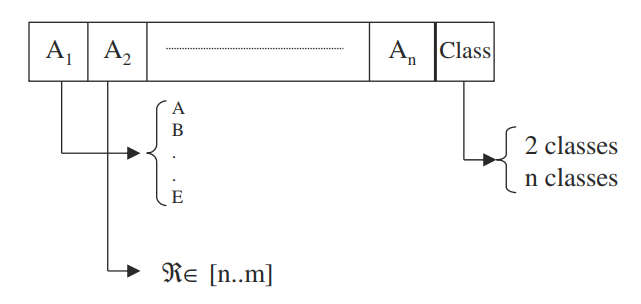
\includegraphics[width=0.4\textwidth]{img/classification_instance.png}
\end{wrapfigure}
Nejprve ještě ke klasifikaci obecně. \textbf{Klasifikační úloha} spočívá v označování předkládaných instancí z nějaké domény správnou \uv{nálepkou}, jejich přiřazení do nějaké \textbf{třídy} (kterých je omezená množina, často pouze dvouprvková). \textbf{Instance} mají pevnou strukturu danou konkrétní problémovou doménou, která se dá vyjádřit pevným počtem \textbf{atributů} (nebo \textit{příznaků, angl. features}), které charakterizují tuto instanci; a v případě anotovaného datasetu má instance jako atribut i správnou třídu. Atributy obecně mohou být nominální (prvek nějaké konečné množiny), diskrétní nebo spojité.


\subsubsection{Pittsburghský přístup}
Pittsburghský přístup je nejbližší klasickému GA. Jedinec v populaci je kompletní množina pravidel řešící daný problém. Tato množina může být různě velká, máme tedy jedince variabilní délky. Při klasifikaci může dojít ke \textit{konfliktu pravidel}, tj. více pravidel může být použito pro klasifikaci dané instance -- to lze řešit např. utříděním pravidel do seznamu, pak se z pravidel \uv{matchujících} danou instanci aplikuje to s nejnižším pořadovým číslem. \textbf{Genetické operátory} jsou poměrně komplikované, typicky jich je více a některé fungují na úrovni celých množin, některé na úrovni jednotlivých pravidel a některé na úrovni termů v pravidlech. 

\textbf{Fitness} jedince se počítá takto: pro každou instanci v trénovací množině se vezme první matchující pravidlo a přiřadí se třída daná tímto pravidlem -- ta se porovná s očekávanou třídou (trénovací vzorky jsou anotované). Fitness je pak dána procentem úspěšně klasifikovaných instancí.

Konkrétním reprezentantem pittsburghského přístupu je například systém GABIL. Ten je určen pro řešení \textit{binární} klasifikace (tj. pouze 3 třídy) a funguje pouze pro domény s \textit{nominálními} atributy. Jednotlivá pravidla (tzv. \textit{komplexy}) jsou ve formátu \textit{predikát $\rightarrow$ třída}, kde predikát je výraz v konjunktivně normální formě (CNF) ve tvaru
$$(A_1 = V_1^1 \lor \dots \lor A_1 = V_1^m) \land \dots \land (A_n = V_n^1 \lor \dots \lor A_n = V_n^m)$$
kde $A_i$ je $i$-tý atribut a $V_i^j$ je $j$-tá hodnota $i$-tého atributu. Taková pravidla lze pak zapsat pomocí binárního řetězce, například 
$$1100|0010|1001|1$$
tedy vyjadřuje pravidlo: pokud první atribut nabývá první či druhé hodnoty, druhý atribut třetí hodnoty a třetí atribut první nebo čtvrté hodnoty, pak instance patří do třídy 1. 

Na těchto binárních řetězcích lze pak snadno aplikovat genetické operátory. Ty fungují na různých úrovních:
\begin{description}
	\leftskip 40pt
	\setlength{\itemsep}{0pt}
	\item[na úrovni jedince (množiny pravidel)] výměna pravidel, kopírování pravidel, generalizace pravidla, smazání pravidla, specializace pravidla, zahrnutí jednoho pozitivního příkladu
	\item[na úrovni komplexů] rozdělení komplexu na 1 selektoru, generalizace selektoru (nahrazení 11\dots1), specializace
	generalizovaného selektoru, zahrnutí negativního příkladu
	\item[na selektorech] mutace $0 \leftrightarrow 1$, rozšíření $0 \rightarrow 1$, zúžení $1 \rightarrow 0$,
\end{description}

\subsubsection{Michiganský přístup}
Zde je jedincem v populaci pravidlo. V klasickém GA typicky dojde ke konvergenci populace k jedinému řešení -- my ale chceme získat množinu pravidel, ideálně docela ortogonálních. Jednou možností je \textbf{Iterative Rule Learning} přístup, který postupně generuje pravidla iterativním spouštěním GA. Tj. spustí se GA, najde se nejlepší pravidlo, to se uloží a z trénovací množiny se odstraní všechny správně klasifikované instance. Toto se opakuje, dokud není trénovací množina prázdná.

Michiganský přístup funguje trochu jinak. Na klasifikaci se podílí \textit{celá populace}. Evoluce neprobíhá po generacích, nýbrž jen občas a jen na části populace. Konkrétně lze rozlišit fázi \textit{objevování nových pravidel} (pomocí GA) a fázi \textit{učení}, během které dochází k odměňování/penalizaci jedinců, jak si vedou při klasifikaci -- od toho je pak odvozena jejich fitness.

Pravidla mohla mít na pravé straně kromě klasifikačního výstupu i další příznaky, tzv \uv{zprávy}. Na levé straně pravidel se pak mohly vyskytovat \uv{receptory} pro jejich příjem. Celý systém má frontu zpráv.

Problémem při klasifikaci celou populací realizace algoritmu odměn pro pravidla. Původní Hollandův návrh obsahoval tzv. \textit{bucket brigade}: pravidla musejí dát část svého \uv{kreditu}, když chtějí soupeřit o možnost být v cestě k řešení. Tento systém byl ale poměrně těžkopádný. 

Zjednodušením tohoto systému byl \textbf{ZCS (Zero Classifier System)}. Neměl vnitřní zprávy ani žádný složitý systém alokace odměn. Síla pravidel se upravovala podle jednoduchého algoritmu:
\begin{itemize}
	\leftskip 20pt
	\setlength{\itemsep}{0pt}
	\item pravidlům, která odpovídají vstupu, ale mají jiný výstup, se síla zmenší násobením konstantou $0 < T < 1$
	\item všem pravidlům se zmenší síla o malou část B
	\item tahle síla se rozdělí rovnoměrně mezi pravidla, která \textit{minule} odpověděla správně, zmenšená o faktor $0<G<1$
	\item nakonec, odpověď od systému se zmenší o B a rozdělí rovnoměrně mezi pravidla, která \textit{teď} odpověděla správně
\end{itemize}
Inovací bylo přidání \textbf{cover} operátoru. Ten řešil případy, kdy nebylo žádné pravidlo pro daný vstup. Pak bylo vygenerováno ad hoc. Pravidla jsou ve formátu $01\#|0$, kde 1 znamená \uv{příznak nastal}, 0 opak a $\#$ je \uv{žolík}. Pro nebinární nominální atributy lze samozřejmě použít rozšířenou abecedu. Ad hoc pravidlo bylo tedy vygenerováno tak, že se nějaké náhodné vstupní atributy nahradily $\#$ a zvolil se náhodný výstup.

Dalším vylepšením byl systém \textbf{XCS}, který zakládá fitness pravidla na jeho přesnosti, nikoliv \uv{výdělku}, tj. dává šanci prosadit se i pravidlům, která vedou k akcím s malou odměnou. Tímto je podpořeno vyvíjení komplexního systému pravidel pokrývajícího co nejvíce případů.




\subsection{Neuroevoluce}
Neuronové sítě se klasicky učí pomocí nějaké varianty backpropagation, ale jsou situace, kdy může být lepší pokusit se vyvinout optimální síť (řešící daný problém) pomocí EA. Mnohdy nelze \textit{učení s učitelem} použít vůbec -- například v robotice -- a je nutno spoléhat na \textit{zpětnovazební učení} (reinforced learning).

Předmětem evoluce mohou být synaptické váhy, struktura sítě, nebo obojí najednou. 

Existují i hybridní přístupy, kdy jsou EA zkombinovány s lokálním prohledáváním. Je například možno pomocí GA najít počáteční vah a poté síť doučit pomocí klasické BP $\rightarrow$ výsledná fitness (BP je citlivé na počáteční nastavení vah).

\subsubsection{Učení vah}
Nejjednodušší je zakódovat váhy do vektoru a pak použít klasický floating point GA se standardními genetickými operátory. Problémy: mnoho parametrů optimalizováno naráz (stovky až tisíce hodnot synaptických vah); různé vzájemně si konkurující kódy reprezentují funkčně totožné sítě; předčasná konvergence. (Jednoduché) křížení navíc nefunguje příliš dobře, neboť výsledné vektory často nekódují validní síť.

\subsubsection{Učení struktury}
Prostor možných architektur je nekonečný a především nediferencovatelný, takže gradientní metody jsou k ničemu. Evoluce však může fungovat bez problémů.
Strukturu sítě lze zakódovat několika způsoby:
\begin{description}
	\leftskip 20pt
	\setlength{\itemsep}{0pt}
	\item[přímé kódování] -- binární matice synapsí, před evolucí se typicky převedou na jeden dlouhý linearizovaný vektor 
	\item[gramatické kódování] 2D formální gramatiky, které jsou \uv{programem} pro vytvoření matice	
	\item[růst sítě ve 2D] rané pokusy v evoluční robotice, velmi neefektivní
	\item[celulární kódování] v podstatě Genetické programování -- program obsahuje instrukce, jak zkonstruovat síť (operace typu: přidej neuron, rozděl neuron sériově/paralelně, přepoj synapsi apod.)
\end{description}

\subsubsection{Evoluce částečných sítí}
\setlength\intextsep{0pt}
\begin{wrapfigure}{r}{0.5\textwidth}
	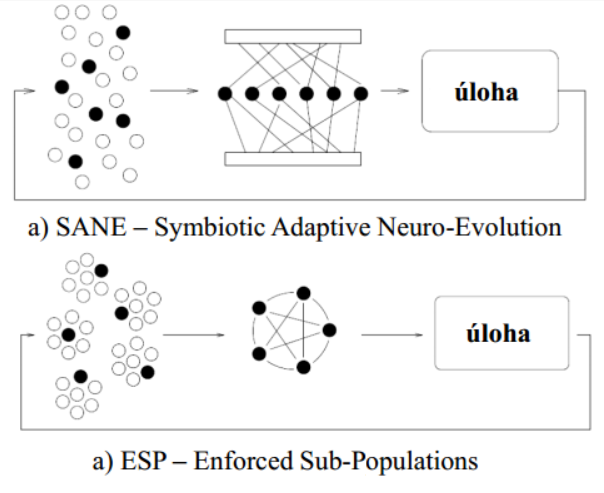
\includegraphics[width=0.5\textwidth]{img/sane_esp.png}
\end{wrapfigure}
\textbf{SANE} (Symbiotic Adaptive Neuroevolution) je variantou neuroevoluce, kdy je struktura pevně daná: jediná skrytá vrstva, pevný počet skrytých neuronů. Jedinci v evoluci jsou neurony (včetně vstupních a výstupních vah). Při ohodnocování se náhodně vybere pevný počet neuronů z populace, postaví se síť a ta se vyhodnotí. Toto se opakuje tak, aby každý neuron z populace byl vybrán aspoň $10\times$. Fitness neuronu je pak průměrná fitness všech sítí, jichž byl součástí.

\textbf{ESP} (Enforced Sub-Populations) funguje na podobném principu, tj. architektura je opět předem daná s pevně daným počtem neuronů (na rozdíl od SANE může být i rekurentní). Rozdíl je v tom, že pro každý z těchto \uv{slotů} se vyvíjejí neurony zvlášť, v oddělených subpopulacích. Takto navržená evoluce podporuje diverzitu (dobrá síť potřebuje různé druhy neuronů), potlačuje redundanci (neurony se vyvíjí pro kompatibilní role) a implicitně rozděluje prohledávaný prostor na podúlohy.


\subsubsection{NEAT (Neuroevolution of Augmenting Topologies)}
Základními charakteristikami algoritmu NEAT jsou: 
\begin{enumerate}
	\leftskip 20pt
	\setlength{\itemsep}{0pt}
	\item evoluce topologie společně s vahami
	\item smysluplné křížení pomocí historických značek
	\item ochrana inovací pomocí druhů
\end{enumerate}
Evoluce topologie zahrnuje přidání/odebrání synapse, přidání/odebrání vrcholu. Typicky se začíná od menší sítě, která postupně roste.

Každý neuron a každý synaptický spoj dostanou při svém vzniku svou \textit{historickou značku} (nebo \uv{rodné číslo}). Tato značka se dědí, takže i u různých potomků lze poznat, zda neurony/spoje mají stejný evoluční původ. Při křížení dvou jedinců se potom postupuje takto: pokud se uzel (neuron či spoj) vyskytuje pouze v jednom rodiči, je automaticky zkopírován; pokud se vyskytuje v obou, je náhodně vybrán jeden z nich.
\begin{figure}[H]
	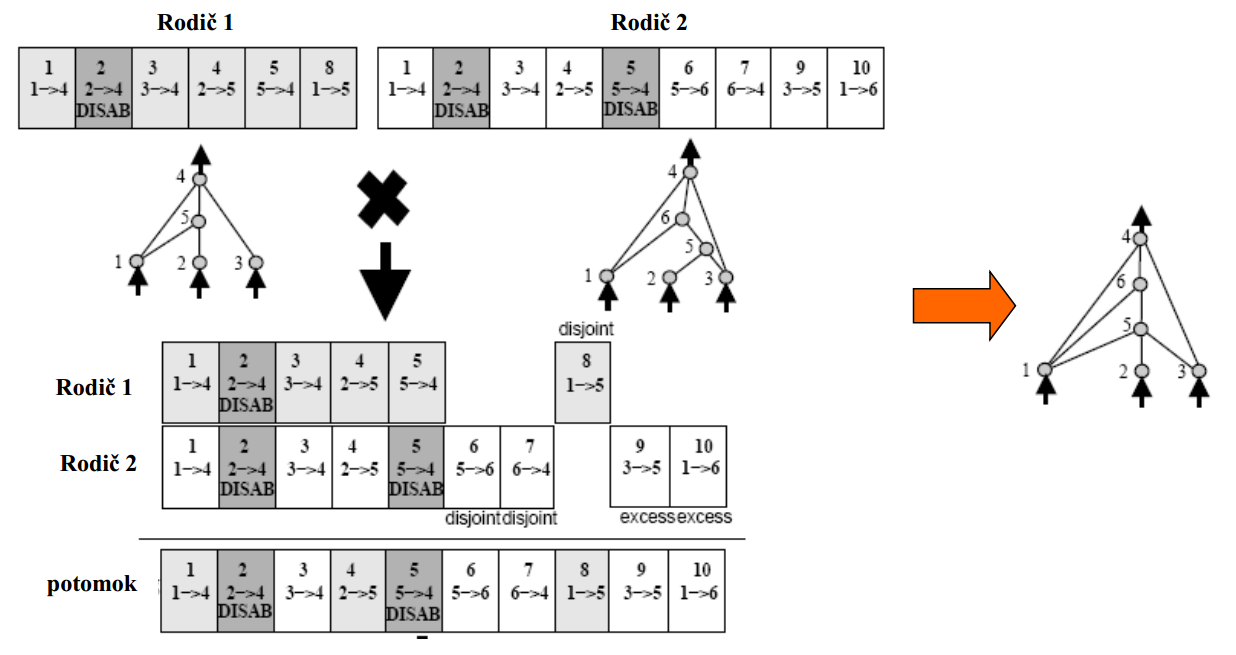
\includegraphics[width=\textwidth]{img/neat.png}
\end{figure}

Když během evoluce vznikne jedinec, který se výrazně liší od ostatních (na to musí být definovaná nějaká metrika), založí se nový \textbf{druh}. Ten je několik generací chráněný -- jedinci nového druhu soutěží pouze mezi sebou.

%TODO hyperneat

\subsection{Řešení kombinatorických úloh}
EA jsou velmi vhodné pro řešení NP-těžkých úloh. Rozebereme několik příkladů:

\subsubsection{Batoh (0-1 knapsack problem)}
\textit{Problém:} máme batoh o kapacitě $CMAX$, množinu $n$ věcí, z nichž každá má cenu $v(i)$ a objem $c(i)$. Úkolem je naplnit batoh tak, abychom maximalizovali sumu cen obsažených věcí a současně nepřekročili kapacitu batohu.

\textbf{Kódování:} Binární jedinci délky $n$, přímočará bitová mapa. Např. 0110010 znamená, že bereme věci s indexy 2,3 a 6. Pozor, jedinci nemusí splňovat podmínku o $CMAX$.

\textbf{Operátory:} Lze použít přímočaré křížení, mutaci a klasickou selekci.

\textbf{Fitness:} Bude mít 2 členy: 
$$\max\limits_{B \subset \{1..n\}} \sum\limits_{i \in B} v(i) \text{\ \ a současně\ \ } \min\limits_{B \subset \{1..n\}} CMAX - \sum\limits_{i \in B} c(i)$$

Problém s víceúčelovou optimalizací lze řešit různě:
\begin{itemize}
	\leftskip 20pt
	\setlength{\itemsep}{0pt}
	\item Oba členy fitness zvážit a sečíst
	\item Použít jeden z obecných EA pro víceúčelové funkce
	\item Anebo chytře změnit zakódování:
	\begin{itemize}	
		\setlength{\itemsep}{0pt}
		\leftskip 20pt
		\item 1 znamená: DEJ věc do batohu POKUD se nepřeplní
		\item takto dosáhneme i toho, že všechny řetězce jsou přípustná řešení
	\end{itemize}
\end{itemize}

\subsubsection{Problém obchodního cestujícího (TSP -- travelling salesman problem)}
\textit{Problém:} Máme $n$ měst, mezi nimi existují cesty definované délky (úplný graf, ohodnocené hrany). Cílem je navštívit všechna města s co nejmenšími náklady -- tj. najít co nejkratší hamiltonovskou kružnici.

\textbf{Fitness:} Délka cesty.

Existuje několik možných reprezentací a na nich závislých genetických operátorů:
\begin{description}
	\leftskip 40pt
	\setlength{\itemsep}{0pt}
	\item[reprezentace sousednosti:] Cesta je seznam měst, město $j$ je na pozici $i$, vede-li cesta z $i$ do $j$. Např. (248397156) odpovídá cestě 1-2-4-3-8-5-9-6-7. Některé seznamy negenerují přípustnou cestu. Klasické křížení nefunguje. Schémata fungují, např (*3*\dots) značí všechny cesty s hranou 2-3.
	\item[reprezentace bufferem] Máme buffer vrcholů, třeba uspořádaný. Reprezentace představuje pořadí města v bufferu, města se z bufferu postupně mažou. Např. buffer (123456789) a reprezentace (112141311) kóduje cestu 1-2-4-3-8-5-9-6-7. V této reprezentaci lze použít jednobodové křížení.
	\item[reprezentace permutací] Nejvíce přímočaré: řetězec (517894623) kóduje cestu 5-1-7-8-9-4-6-2-3. Klasické křížení nefunguje, byly navrženy speciální operátory (dobrý přehled viz \footnote{http://www.rubicite.com/Tutorials/GeneticAlgorithms/CrossoverOperators/PMXCrossoverOperator.aspx}):
	\begin{description}
		\leftskip 30pt
		\setlength{\itemsep}{0pt}
		\item[PMX (partially mapped crossover] Náhodně vybereme podřetězec z rodiče 1, ten zkopírujeme do nového jedince. Pak se podíváme na tytéž pozice v rodiči 2. Pro každou hodnotu, která se ještě nevyskytuje v budovaném potomkovi, budeme hledat vhodné umístění: nechť chceme umístit hodnotu $h$, která se nachází v rodiči 2 na pozici $i$. Vezmeme hodnotu $h_2$ na téže pozici $i$, ale v rodiči 1. Pak se podíváme, kde se $h_2$ nachází v rodiči 2 -- označme tuto pozici jako $i_2$. Je-li to mimo zkopírovanou oblast, pak jsme našli vhodné umístění a zkopírujeme původní hodnotu $h$ do nového potomka na $i_2$. Je-li $i_2$ uvnitř kopírovaného intervalu, pak pokračujeme v hledání -- do $h_2$ dosadíme hodnotu na $i_2$ v rodiči 1. Viz obr. \ref{pmx}.
		\begin{figure}[H]
			\centering			
			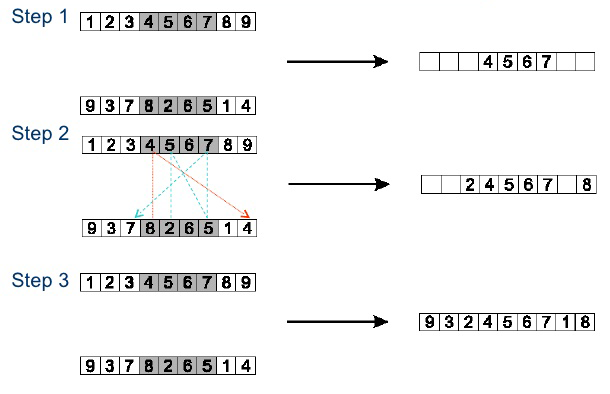
\includegraphics[width=0.6\textwidth]{img/pmx.png}
			\caption{Partially mapped crossover (PMX)}
			\label{pmx}
			
		\end{figure}
		\item[OX (order crossover)] Nejrychlejší křížení. Stejně jako v PMX nejprve vezmeme náhodný podinterval rodiče 1 a beze změny jej zkopírujeme do potomka. Poté vezmeme nepoužité hodnoty z rodiče 2 a počínaje pravým koncem zkopírovaného intervalu je dokopírujeme do potomka.
		
		\begin{figure}[H]
			\centering			
			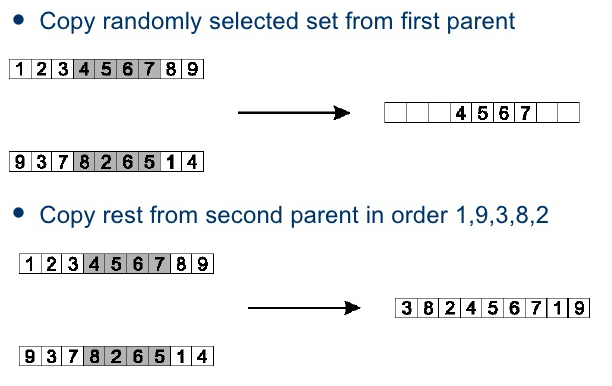
\includegraphics[width=0.6\textwidth]{img/ox.png}
			\caption{Order crossover (OX)}
			\label{pmx}
			
		\end{figure}
		\item[CX (cyclic crossover)] Nejprve jsou identifikovány \uv{cykly} mezi dvěma rodiči: začneme první hodnotou v prvním rodiči, podíváme se na hodnotu na tomtéž indexu v rodiči 2, tuto hodnotu najdeme v rodiči 1, podíváme se na hodnotu na témže indexu v rodiči 2 atd. dokud neuzavřeme cyklus. Takto najdeme všechny cykly. Nového jedince pak vytvoříme kopírováním hodnot po cyklech: hodnoty z prvního cyklu zkopírujeme z prvního rodiče, hodnoty z druhého cyklu z druhého rodiče, hodnoty z třetího cyklu opět z prvního rodiče atd.
		
		\begin{figure}[H]
			\centering			
			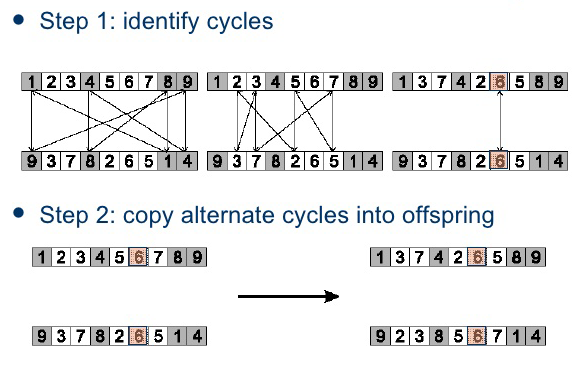
\includegraphics[width=0.6\textwidth]{img/cx.png}
			\caption{Cyclic crossover (CX)}
			\label{cx}
			
		\end{figure}
		
		\item[ER (edge recombination)] Pro každé město si udělám seznam hran, které do/z něj vedou a jsou použity v některém z rodičů. Pak začnu náhodným městem a postupně napojuji další, přičemž vždy ze sousedů vybírám město s nejméně hranami (v případě shody náhodně). Může se stát, že nelze hranu vybrat, ale to se v praxi stává zřídka.
		\item[ER2] Vylepšení: označím si hrany, které jsou dvakrát (tj. v obou rodičích) a při výběru jim dávám přednost. To zachovává ještě více hran z obou rodičů.
		\begin{figure}[H]
			\centering			
			\smallskip
			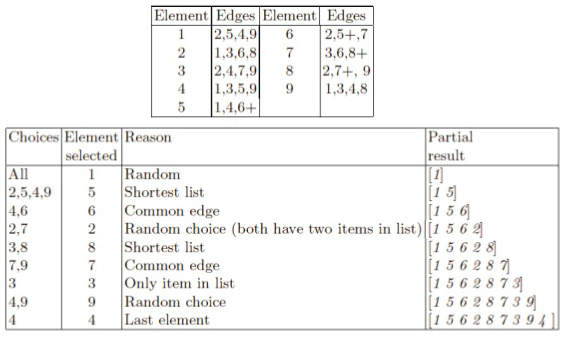
\includegraphics[width=0.6\textwidth]{img/er.png}
			\caption{Edge recombination 2 (ER2): příklad pro rodiče (123456789) a (937826514)}
			\label{pmx}
			
		\end{figure}
		
	\end{description}
\end{description}



Mutace jsou obecně jednodušší (pro všechny reprezentace), používá se:
\begin{itemize}
	\leftskip 20pt
	\setlength{\itemsep}{0pt}
	\item inverze podcesty
	\item posun podcesty
	\item záměna 2 měst
	\item záměna podcest
	\item složitější heuristiky: např. \textbf{2-OPT}. Tento \uv{chytrý operátor} funguje tak, že se vyberou dvě hrany, ty se odeberou a nahradí jinými dvěma hranami (je jen jedna možnost). Nakonec se vybere kratší z obou vzniklých cest. Vlastně se jedná o mutaci, která vezme část cesty a tu vloží do jedince v opačném pořadí. 2-OPT se navíc ještě podívá, jestli je výsledek kratší a přijme ho jen pokud je.
	
	2-OPT se přirozeně dá zobecnit na \textbf{$k$-OPT}, odstraní se $k$ hran a vzniklé fragmenty se pospojují tak, aby výsledná cesta byla co možná nejkratší.
\end{itemize}

Úspěšnost evoluce závisí také na inicializaci. Nejpoužívanější jsou dvě varianty:
\begin{description}
	\leftskip 40pt
	\setlength{\itemsep}{0pt}
	\item[nejbližší sousedi] Začni s náhodným městem, postupně vybírej jako další to nejbližší z dosud nevybraných.
	\item[vkládání hran] Budujeme cestu T, na začátku náhodná hrana. K cestě T vyber nejbližší město c mimo T. Najdi hranu k-j v T tak, že minimalizuje rozdíl mezi k-c-j a k-j. Vyhoď k-j, vlož k-c-j do T.
\end{description}

\subsection{Vícekriteriální optimalizace (MOEA -- Multi-objective EA)}
Velmi často potřebujeme optimalizovat více funkcí současně, tj. místo jedné fitness jich máme celý vektor $\overline{f} = (f_1, f_2, \dots f_n)$. Ty si často odporují, nelze tedy najít řešení optimální pro všechny zároveň.

\begin{wrapfigure}{r}{0.45\textwidth}
	\centering
	
	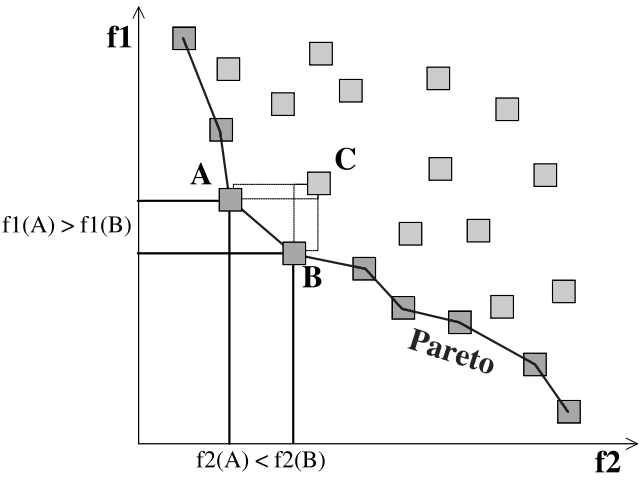
\includegraphics[width=0.4\textwidth]{img/pareto.png}
\end{wrapfigure}

Řekneme, že řešení $x$ \textbf{slabě dominuje} řešení $y$, jestliže $x$ je ve všech kritériích aspoň tak dobré jako $y$, tj. $f_i(x) \leq f_i(y)\quad \forall i \in \{1,\dots,n\}$. 

Řekneme, že $x$ \textbf{dominuje} $y$, když jej slabě dominuje a navíc je aspoň v jedno kritériu lepší, tj. $\exists j: f_j(x) < f_j(y)$. 

Řešení $x$ a $y$ jsou \textbf{nesrovnatelná}, jestliže $x$ nedominuje $y$ a $y$ nedominuje $x$.

\textbf{Pareto-optimální řešení} (Paretova fronta, Pareto-optimální fronta) je množina jedinců, kteří nejsou dominováni žádným jiným jedincem. Je často nekonečná, hledáme konečnou aproximaci.

V případě MOEA není jeden nejlepší jedinec v populaci, používá se celá populace a považuje se za aktuální aproximaci Pareto-optimální množiny řešení. 

\subsubsection{Algoritmy}
Hlavní rozdíl mezi jednokriteriálními a vícekriteriálními algoritmy je v selekci (operátory mohou klidně zůstat stejné). S čímž samozřejmě souvisí způsob, jakým se počítá fitness. Celkově je potřeba zajistit konvergenci k Pareto optimální frontě a zároveň zajistit i dobré pokrytí této fronty.
\begin{description}
	\leftskip 40pt
	\setlength{\itemsep}{0pt}
	\item[Agregace fitness] Nejjednodušší přístup. Definujeme agregovanou fitness $f$ jako váženou sumu všech $f_i$ a problém řešíme jako klasickou jednokriteriální optimalizaci. Problémem je nastavení vah u jednotlivých $f_i$.
	\item[VEGA (Vector Evaluated GA)] Populaci $N$ jedinců utřídím podle každé z $n$ fitness funkcí, poté pro každé $i$ vyberu $\frac{N}{n}$ nejlepších jedinců dle $f_i$. Na ty poté aplikuji křížení, mutaci a provedu selekci do další generace. 
	
	Nevýhodou tohoto přístupu je obtížné udržování diverzity populace a často dochází ke konvergenci k extrémům jednotlivých $f_i$.
	\item[NSGA (Non-dominated sorting GA)] Fitness se počítá pomocí dominance, diverzitu populace zaručuje \textbf{niching}.
	
	Populace $P$ je rozdělena na postupně konstruované fronty $F_1$, $F_2$, \dots, a to takto: 
	\begin{itemize}
		\leftskip 40pt
		\setlength{\itemsep}{0pt}
		\item $F_1$ je množina všech nedominovaných jedinců z $P$
		\item $F_2$ je množina všech nedominovaných jedinců z $P-F_1$
		\item $F_3$ je množina všech nedominovaných jedinců z $P - (F_1 \cup F_2)$
		\item \dots
	\end{itemize}
	
	Pro každého jedince $i$ ve frontě $F_k$ se spočte jeho \textit{niching faktor} jako
	$$sh(i) = \sum_{j \in F_k} sh(i,j)$$
	kde 
	$$
	sh(i,j) = 
	\begin{cases}
		1 - \left(\frac{d(i,j)}{dshare}\right)^2 	& \quad \text{pro $d(i,j) < dshare$} \\
		0 											& \quad \text{jinak}\\
	\end{cases}
	$$
	kde $d(i,j)$ je vzdálenost $i$ a $j$, $dshare$ je předem daný parametr. Niching faktor tedy vyjadřuje, jak blízko jsou další jedinci v populaci. Čím blíže 0, tím osamocenější jedinec je, naopak hodnota blízká 1 znamená mnoho blízkých sousedů.
	
	Jedinci z $F_1$ dostanou nějakou \uv{dummy fitness} dělenou jejich niching faktorem. Jedinci z $F_2$ dostanou jinou dummy fitness, která je menší než fitness nejhoršího jedince z $F_1$ a opět se dělí jejich niching faktorem; atd.
	
	\item[NSGA II] Odstraňuje nutnost určení $dshare$ -- nahrazuje ji \textbf{crowding distance}, což je součet přes všechna kritéria, vzdálenosti nejbližšího horšího (v daném kritériu) a nejbližšího lepšího jedince. Fitness se pak ve skutečnosti nepočítá, namísto toho se v turnajové selekci porovnávají jedinci nejprve podle čísla fronty (menší je lepší), v případě remízy podle crowding distance (větší je lepší -- jedinci jsou v řídce osídlené oblasti a tedy lépe přispívají k pokrytí fronty).
	
	Dále zavádí elitismus: stará a nová generace jsou spojeny, utříděny a z nich se pak vybírá lepší část do další populace. Postupně se kopírují fronty (od nejlepší) dokud se vejdou do populace, z fronty, která se již nevejde celá, se vybírá podle turnajové metody popsané výše.
	
\end{description}

\subsubsection{Porovnání algoritmů}
Pro porovnání kvality řešení dvou různých algoritmů je třeba vyhodnotit, která z výsledných populací lépe aproximuje Pareto optimální množinu. 
\begin{description}
	\leftskip 40pt
	\setlength{\itemsep}{0pt}
	\item[IGD (Inverted Generational Distance)] IGD měří průměrnou vzdálenost každého řeše\-ní na \textit{skutečné} Pareto optimální frontě k nejbližšímu řešení ve výsledné množině. Díky tomu indikátor vyjadřuje jak blízkost řešení k Pareto-optimální frontě (convergence), tak to, jestli jsou řešení po frontě rozmístěna rovnoměrně (spread). Menší hodnoty tohoto indikátoru jsou lepší. 
	\begin{figure}[H]
		\centering
		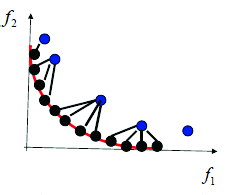
\includegraphics[width=0.4\textwidth]{img/igd.png}
	\end{figure}
	
	\item[Hyperobjem (HV -- hypervolume)] Hyperobjem vyjadřuje objem prostoru dominovaného danou množinou (a omezeného zvoleným referenčním bodem). V případě, že máme jen dvě funkce, které obě najednou minimalizujeme, tak se jedná o plochu \uv{nad} body, které jsou obrazy jedinců v populaci. Plocha je shora omezena referenčním bodem (jinak by byla nekonečná). Tento indikátor opět spojuje jak konvergenci, tak pokrytí Pareto-optimální fronty. Větší hodnoty tohoto indikátoru jsou lepší. Někdy se také jako indikátor používá rozdíl hyperobjemu \textit{skutečné} Pareto optimální fronty a aproximace nalezené algoritmem. Potom jsou samozřejmě lepší menší hodnoty.
	\begin{figure}[H]
		\centering
		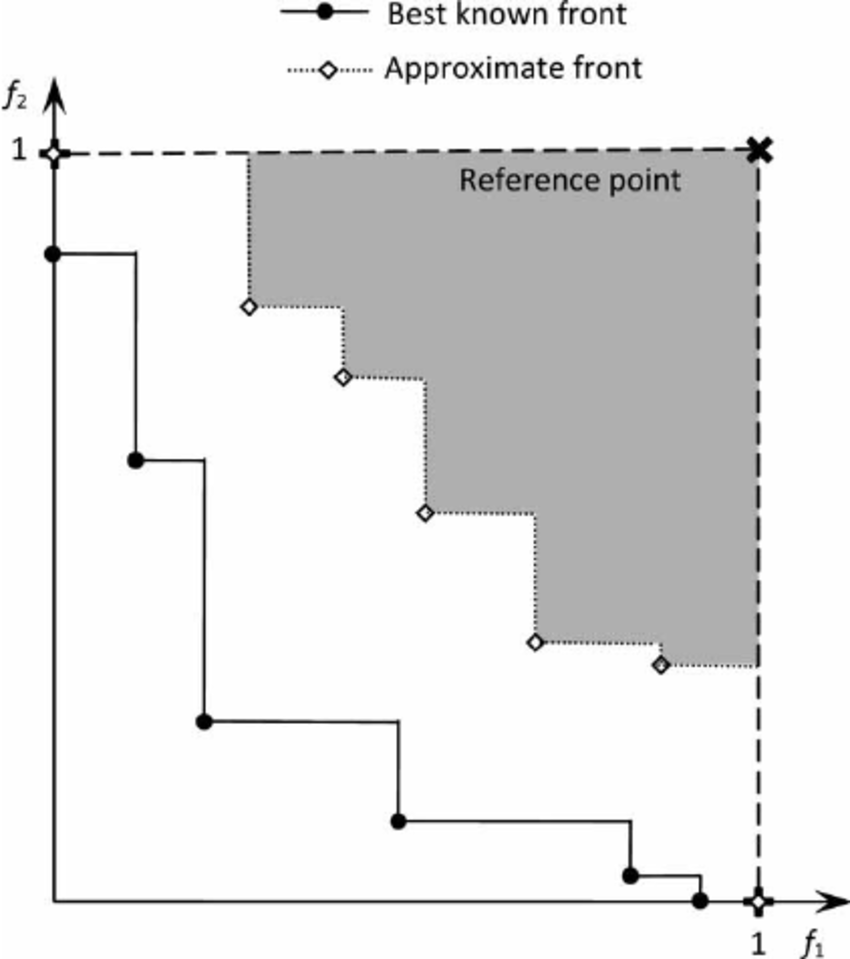
\includegraphics[width=0.35\textwidth]{img/hypervolume.png}
	\end{figure}
	
\end{description}


\part{Strojové učení}
\chapter{Strojové učení a jeho aplikace}
\section{Strojové učení; prohledávání prostoru verzí, učení s učitelem a bez učitele, pravděpodobnostní přístupy, teoretické aspekty strojového učení.}
\subsection{Teoretické aspekty strojového učení}

\subsubsection{Základní pojmy}
\begin{itemize}
	\item cílová veličina $Y$ -- kvantitativní nebo kategoriální
	\item příznaky (features) $X$ 
	\item předpokládáme, že v datech existuje vztah $f$, pro nějž $Y = f(X) + \epsilon$. Chceme sestrojit model $\hat{f}$, který co nejlépe aproximuje $f$. 
	\item modely
	\begin{itemize}
		\item parametrické (např. lin. regrese) 
		\item neparametrické modely (např. $k$-NN)
	\end{itemize}
	
	\item učení
	\begin{itemize}
		\item s učitelem (supervised) -- máme cílovou veličinu, kterou se snažíme aproximovat
		\item bez učitele (unsupervised) -- popis dat, klastrování
	\end{itemize}
	
	\item data rozdělíme na
	\begin{itemize}
		\item trénovací
		\item testovací
		\item (validační) -- pro doladění parametrů (např. volba stupně polynomu)
	\end{itemize}
	Používá se poměr 2/3 : 1/3 (bez validační množiny), nebo 1/2 : 1/4 : 1/4 (s validační).
	
	\textbf{Stratifikovaný výběr:} data rozdělíme tak, aby v každé části byl zachován poměr tříd.
	\item úspěšnost klasifikace:
	\bigskip
	\begin{table}[H]
		\centering
		\begin{tabular}{|c|c|c|}
			\hline
			správná třída \textbackslash klasifikace & + & - \\ \hline
			+ & TP (true positive) & FN (false negative) \\ \hline
			- & FP (false positive) & TN (true negative) \\ \hline
		\end{tabular}
	\end{table}
	\bigskip
	\begin{table}[H]
		\centering
		\begin{tabular}{|c|c|c|}
			\hline
			celková správnost & accuracy & $Acc = \frac{TP + TN}{TP + TN + FP + FN}$ \\ \hline
			chyba & error & $Err = \frac{FP + FN}{TP + TN + FP + FN}$ \\ \hline
			přesnost & precision & $Prec = \frac{TP}{TP + FP}$ \\ \hline
			úplnost, sensitiva & recall, sensitivity & $Rec = \frac{TP}{TP + FN}$ \\ \hline
			specificita & specificity & $Spec = \frac{TN}{TN + FP}$ \\ \hline
		\end{tabular}
	\end{table}
	
	
\end{itemize}

\subsubsection{Chyba}
Očekávaná hodnota:
$$E(Y-\hat{Y})^2 = E[f(X) + \epsilon - \hat{f}(X)]^2$$

\begin{itemize}		
	\item reducibilní chyba ($[f(X) - \hat{f}(X)]^2$ -- špatně naučený model
	\item ireducibilní chyba($Var(\epsilon)$)-- vliv neměřených veličin, náhody, šumu v datech 
\end{itemize}

\paragraph{Míry chyby pro regresi}
\begin{itemize}
	\item \textbf{kvadratická} $L(Y, \hat{f}(X)) = (Y - \hat{f}(X))^2 $
	\item \textbf{absolutní} $L(Y, \hat{f}(X)) = |Y - \hat{f}(X)| $	
\end{itemize}
\paragraph{Míry chyby pro klasifikaci}
Cílovou veličinu označujeme většinou $G$ (místo $Y$), model predikuje buď jednu konkrétní třídu, nebo pravděpodobnostní vektor různých tříd $p_k(X) = P(G=k|X)$.
\begin{itemize}
	\item \textbf{0-1 chyba} $L(G,\hat{G}(X)) = I(G \neq \hat{G}(X))$
	\item \textbf{log-likelihood} $L(G,\hat{p}(X)) = -2\sum_{k=1}^{K}I(G=k)\cdot \log \hat{p}_k(X) = -2\log \hat{p}_G(X)$
\end{itemize}

\textbf{Trénovací chyba} na trénovacích datech velikosti $N$ je 
$$\overline{err} = \frac{1}{N}\sum_{i=1}^{N}L(y_i, \hat{f}(x_i))$$

\textbf{Chyba generalizace} je očekávaná chyba na nezávislých testovacích datech $(X,Y)$
$$Err = E[L(Y,\hat{f}(X))]$$

Odhad chyby generalizace na testovacích datech $S = (X,Y)$:
$$\overline{Err} = \frac{1}{T}\sum_{i=1}^{T}L(y_i, \hat{f}(x_i))$$
resp.
$$\overline{Err} = \frac{1}{T}\sum_{i=1}^{T}L(g_i, \hat{p}(x_i))$$

\subsubsection{Přeučení, bias-variance trade-off}
Přeučení na trénovacích datech $\to$ zvýšení chyby na testovacích.

Jiné vyjádření chyby:
$$E(Y - \hat{X})^2 = Var(\hat{X}) + [Bias(\hat{f}(X))]^2 + Var(\epsilon)$$

\textbf{Bias:} chybné předpoklady učícího algoritmu, zjednodušení reálného světa. Např. použití lineární regrese pro nelineární data má velký Bias ($\to$ underfitting)

\textbf{Variance:} jak moc se $\hat{f}$ změní pro jiná trénovací data. Pokud je moc velká, znamená to, že model kromě relevantních vztahů modeluje i šum v datech ($\to$ přeučení).

Vztah: čím flexibilnější model, tím nižší bias, ale vyšší variance.

\subsubsection{Prokletí dimenzionality}
\url{http://www.visiondummy.com/2014/04/curse-dimensionality-affect-classification/}
\uv{Nejbližší sousedé jsou při velké dimenzi hodně daleko.}

Zvyšování počtu příznaků (tedy dimenzionality $X$) vede k exponenciálnímu snížení hustoty vzorků ve vstupním prostoru. 

Problém: přeučení -- při dostatečně velké dimenzi lze vždycky najít dělící nadrovinu.

Problém: chceme získat dostatek trénovacích dat, abychom pokryli řekněme 20\,\% rozsahu každého příznaku. Pro 1D stačí 20\,\% dostupných dat, pro 2D už potřebujeme 45\,\%, pro 3D 58\,\%.

\subsubsection{Krosvalidace}
Používá se typicky v případě nedostatku dat, kdy nelze vyčlenit testovací množinu. Případně pro stabilnější odhad chyby.

Data se rozdělí na $k$ částí (folds), jedna část se použíje pro testování, ostatní pro učení. Opakujeme s každou částí, získáme $k$ testů, jejich výsledky zprůměrujeme. Ze zkušenosti se používá $k = 5$ nebo $k = 10$. 

Celý proces se často opakuje pro různá dělení (aby se ošetřila možnost nešťastného dělení), častá je \uv{$10 \times 10$fold crossvalidation}

Kritika: odhady chyby nejsou nezávislé.

\subsubsection{LOOCV (Leave-one-out cross-validation)}
Jeden vzorek dáme stranou, naučíme model, poté otestujeme na odloženém vzorku. Zprůměrujeme chybu. Vlastně ekvivalentní $N$-fold CV, tj. každý vzorek ve vlastním foldu. 

Výhody: velká trénovací množina, učení netřeba opakovat (dělení je jednoznačné).

Nevýhody: výpočetně náročné, může selhat (např. dvě třídy, data 50 na 50 -- chyba je 100\,\%!)

\subsubsection{Bootstrap}
Máme $N$ vzorků, z nich vybereme \textit{s opakováním} $N$ vzorků do trénovací množiny (tj. některé tam budou víckrát, některé vůbec). Vzorky, které nebyly vybrány, použijeme jako testovací množiny (pravděpodobnost nevybrání = $(1-\frac{1}{N})^N \approx e^{-1} =0.368$).

Provedeme mnoho bootstrap výběrů a celkovou chybu spočteme jako 
$$\overline{Err}^{(1)} = \frac{1}{N}\sum_{i=1}^{N}\frac{1}{|C^{-i}|}\sum_{b\in C^{-i}} L(y_i, \hat{f}^{b}(x_i))$$
kde $C^{-1}$ je množina bootstrap výběrů nebosahujících vzorek $i$.

Takto formulovaná chyba je pesimistická, neboť učíme na $N$ datech, která ale reálně pocházejí pouze z 0.632$N$ dat, proto korekce přičtením chyby na trénovacích datech:

$$\overline{Err}^{(0.632)} = 0.632\cdot \overline{Err}^{(1)} + 0.368 \cdot \overline{err}$$

Tato chyba zase ale může podhodnotit v případě přeučených dat, proto 

$$\overline{Err}^{(0.632+)} = \hat{w}\cdot \overline{Err}^{(1)} + (1-\hat{w})\cdot \overline{err}$$
kde
$$w = \frac{0.632}{1 - 0.368\cdot\hat{R}}
\quad \text{kde}\quad 
\hat{R} = \frac{\overline{Err}^{(1)} - \overline{err}}{\hat{\gamma} - \overline{err}}
\quad \text{kde}\quad 
\hat{\gamma} = \frac{1}{N^2}\sum_{i=1}^{N}\sum_{j=1}^{N}L(y_i,\hat{f}(x_j))
$$


regularizace: p >> n
* subset selection
* shrinkage (ridge, lasso)
* dimension reduction (PCA, PCR, PLS)


\subsection{Učení s učitelem}
\subsubsection{Lineární regrese}
Předpokládáme lineární vztah, tj. $Y \approx \beta_0 + \beta_1 X$. Náš model bude tedy $\hat{y} = \hat{\beta}_0 + \hat{\beta}_1 x$. 

Odhadneme $\hat{\beta}_0, \hat{\beta}_1$ z dat: 
\begin{itemize}
	\item definujeme \textbf{residuum} vzorku jako $y_i - \hat{y}_i = y_i - (\hat\beta_0 + \hat\beta_1x_i)$
	\item \textbf{RSS (residual sum of squares)} = $e_1^2 + e_2^2 + \dots + e_n^2$
	\item RSS chceme minimalizovat (=MSE, minimal square error), takže zderivujeme a položíme rovno 0. Dostaneme
	$$\hat\beta_1 = \frac{\sum_{i=1}^{n}(x_i-\overline{x})(y_i - \overline{y})}{\sum_{i=1}^{n}(x_i-\overline{x})^2}
	\qquad
	\hat\beta_0 = \overline{y} - \hat\beta_1\overline{x}$$
	\item ve skutečnosti: $Y =\beta_0 + \beta_1 X + \epsilon$, kde $\epsilon$ je chyba modelu, vliv jiných proměnných, šum,...	
\end{itemize}

\paragraph{Přesnost odhadu koeficientů}
Značení: $\beta_1, \beta_0$ jsou reálné koeficienty, $\hat{\beta}_1, \hat{\beta}_0$ jsou odhady získané pomocí MSE.

Standardní chyba:
$$
SE(\hat{\beta}_1)^2 = \frac{\delta^2}{\sum_{i=1}^{n}(x_i - \overline{x})}
\qquad
SE(\hat{\beta}_0)^2 = \delta^2 \left[\frac{1}{n} + \frac{\overline{x}^2}{\sum_{i=1}^{n}(x_i - \overline{x})} \right]$$

kde $\delta^2 = Var(\epsilon)$, taktéž označován jako RSE (standard residual error). Odhaduje se jako $RSE = \sqrt{RSS/(n-2}$.

\subparagraph{Intervaly věrohodnosti:} na 95\,\% leží $\beta_1$ v intervalu $[\hat{\beta}_1 - 2\cdot SE(\hat{\beta}_1), \hat{\beta}_1 + 2\cdot SE(\hat{\beta}_1)]$, analogicky $\beta_0$.

\subparagraph{Testování hypotézy nezávislosti}
Nulová hypotéza $H_0: \beta_1 = 0$ (žádná závislost $Y$ na $X$).

Alternativní hypotéza $H_1: \beta_1 \neq 0$ (existuje závislost $Y$ na $X$).

Používá se \textbf{t-statistika}: $t = \frac{\hat\beta_1 - 0}{SE(\hat\beta_1)}$. Porovnáním s tabelovaným t-rozložením pro $(n-2)$ stupňů volnosti získáme \textbf{p-value}, pokud je $< 0.05$, zamítáme nulovou hypotézu.

\paragraph{Správnost modelu}
Chceme-li ohodnotit, jak dobře model odpovídá datům, můžeme použít
\begin{itemize}
	\item $RSE = \sqrt{RSS / (n-2)}$ Tato míra však závisí na datech, těžko se porovnává pro různá data.
	
	\item $R^2 = \frac{TSS - RSS}{TSS}$, kde $RSS = \sum_{i=1}^{n}(y_i - \hat{y}_i)^2$ a $TSS = \sum_{i=1}^{n}(y_i - \overline{y})^2$ (total sum of squares). Hodnota TSS vyjadřuje rozptyl v Y, RSS je rozptyl, který zůstal \uv{nevysvětlen} regresí; TSS - RSS je pak rozptyl v Y, který \uv{vysvětluje} regrese. $R^2$ tedy vyjadřuje \textbf{kolik procent rozptylu v $Y$ lze vysvětlit pomocí $X$}.
\end{itemize}
\paragraph{Vícerozměrná lineární regrese}
Vícerozměrná lineární funkce, tj. $Y = \beta_0 + \beta_1X_1 + \beta_2X_2 + \dots + \beta_px_p + \epsilon$. Náš model bude tedy $\hat{y} = \hat{\beta}_0 + \sum_{i=1}^{n}X_i\hat{\beta}_i$. Rozšíříme li vektory $x$ na $x = \langle1, x_1, x_2,\dots\rangle$, můžeme psát maticově:
$$\hat{y} = X\beta$$

Pro odhad parametrů $\beta$ použijeme opět RSS:
$$RSS(\beta) = \sum_{i=1}^{N}(y_i - x_i^T\beta)^2 = (y-X\beta)^T(y-X\beta)$$
Derivací podle $\beta$ dostaneme $X^T(y-X\beta) = 0$. Pro regulární matice vyjde $\hat{\beta} = (X^TX)^{-1}X^Ty$, pro singulární zkoušíme ubrat závislé sloupce.
		

\paragraph{Další varianty}
\begin{itemize}
\item \textbf{kvalitativní proměnné (prediktory):} Používáme \uv{dummy} proměnné, pro 0/1 stačí 1 dummy, pro $k$ tříd je třeba $k-1$ dummy proměnných.

\item \textbf{nelineární modely} Polynomiální, exponenciální, logaritmické, součiny prediktorů
\end{itemize}

\paragraph{Problémy}
\begin{itemize}
	\item \textbf{korelovaná rezidua:} např. u časových řad mívají sousedé často podobnou chybu (směr, velikost), což může vést k celkovému podhodnocení chyby.
	
	\item \textbf{nekonstantní rozptyl reziduí:} např. s rostoucím $x$ roste rozptyl. Řešením je logaritmická transformace vstupu nebo použití vážených nejmenších čtverců.
	
	\item \textbf{outliers (odehlá pozorování):} Chyba v datech (odstranit) nebo v modelu (chybějící prediktor)? Většinou moc nepohne s přímkou, ale vede ke zkreslení chyby, p-hodnoty,... 
	
	\item \textbf{high leverage point:} Vzdálený bod, nezvyklé $x_i$, může silně ovlivnit přímku. Při vícerozměrné regresi není lehké odhalit, pomůže \textit{leverage statistics}.
	
	\item \textbf{kolinearita}
\end{itemize}

\subsubsection{Lineární metody pro klasifikaci (logistická regrese, LDA, QDA)}
  \begin{itemize}
	\item klasifikace: kvalitativní cílová proměnná $G$, předpověz správnou $G_k \in G$ nebo $p_k = P(G=G_k | X)$
	\item LINEÁRNÍ metody = hranice mezi třídami je linární
	\item NE lineární regrese:
	\begin{itemize}
		\item číselné kódování je špatně (není přirozené pořadí, škála; jiná pořadí mohou dát jiné výsledky)
		\item pro bin. G by šlo, ale logistická je lepší (žádné negativní pravděpodobnosti)
		\item masking = nějaká třída je skryta ostatními, nikdy nedominuje
	\end{itemize}
	\end{itemize}
	\paragraph{Logistická regrese}
	Předpokládáme binární klasifikaci, tj. dvě třídy 0 a 1. Chceme modelovat vztah mezi $p_k(X) = P(G=1 | X)$ a $X$. Tj. chceme fci, jejíž hodnoty jsou vždy mezi 0 a 1 (což lin. není). Použijeme \textbf{logistickou funkci}:
	$$p(X) = P(G=1 | X) = \frac{\exp(\beta_0 + \beta_1X)}{1 + \exp(\beta_0 + \beta_1 X)}$$
	
	resp. od ní odvozenou \textbf{logit funkci}
	$$\log\frac{p(X)}{1 - p(X)} = \beta_0 + \beta_1 X$$
	Levá strana této rovnice se nazývá \textit{logit} nebo \textit{log-odds} (protože $p(X)/(1-p(X))$ se nazývá \textit{\uv{šance} = odds}). 
	
	\subparagraph{Učení koeficientů}
	Pro naučení parametrů modelu $\beta$ se používá \textit{maximalizace věrohodnosti}, kde optimalizovaná funkce má tvar $$l(\beta_0,\beta_1) = \prod_{i : y_i = 1} p(x_i) \cdot \prod_{i : y_i = 0} (1-p(x_i))$$
	
	Kvalitativní prediktory lze řešit dummy proměnnými stejně jako u lin. regrese.

	\subparagraph{Více rozměrná logistická regrese}
	Více prediktorů:
	$$p(X) = \frac{\exp(\beta_0 + \beta_1X_1 + \dots + \beta_pX_p)}{1 + \exp(\beta_0 + \beta_1 X_ + \dots + \beta_pX_p)}$$
	
	Více cílových tříd: existuje, spíše se ale používá LDA.

	\paragraph{LDA (Linear Discriminant Analysis)}
	\begin{itemize}
		\item use of bayes theorem
		\item předpoklad normálního rozložení X
		\begin{itemize} 
			\item každá třída vlastní mean, ale společná kovarianční matice (kovariance mezi prediktory) $\to$ stejně tvarované elipsy
		\end{itemize}
		\item aproximuje bayesovský klasifikátor (=ideální klasifikátor při znalosti tříd)
		\item různá cena chyby -\textgreater{} posun hranice z 0.5 třeba na 0.2
		\item ROC křivka
	\end{itemize}
	\paragraph{QDA (Quadratic Discriminant Analysis)}
	\begin{itemize}
		\item každá třída svou kovarianční matici $\to$ různé elipsy
		\item mnohem více parametrů, které je třeba odhadnout z dat 
		\item kvadratická hranice
	\end{itemize}
	
	\paragraph{Srovnání (kNN, logistická regrese, LDA, QDA)}
	\begin{itemize}	
		\item LDA, QDA \dots předpoklad norm. rozložení
		\item logist, LDA \dots lin. rozh. hranice
		\item kNN \dots vhodné pro libovolně nelineární hranici
	\end{itemize}


\subsubsection{Rozhodovací stromy}
Rozhodovací strom pro daný cílový atribut $G$ je kořenový strom tvořený z 
\begin{itemize}
	\item \textit{kořene a vnitřních listů označených atributem}, ze kterého vede jedna hrana pro každou možnou hodnotu tohoto atributu (případně interval pro spojité predikáty)
	\item \textit{listů označených předpokládanou hodnotou cílového atributu G} za předpokladu, že ostatní atributy nabývají hodnot daných uzly na cestě od kořene do tohoto listu
\end{itemize}

\textbf{Základní algoritmus (obecně):}
\begin{enumerate}
	\item vyber atribut, vytvoř uzel a rozděl data podle hodnoty atributu (pro regresi: nový dělicí bod intervalu)
	\item pro každou hodnotu vytvoř podstrom z dat s odpovídající hodnotou
	\item pokud data obsahují jen jednu hodnotu $G$ nebo pokud došly atributy k dělení, \textit{vytvoř list s hodnotou nejčetnější cílové třídy}
\end{enumerate}

Stromy mohou být
\begin{itemize}
	\item \textbf{regresní} -- list obsahuje průměr hodnot cílové veličiny v regionu daném atributy ($\to$ schodovitý graf). Jako míru chyby lze použít RSS.
	
	\item \textbf{klasifikační} -- list obsahuje najčetnější třídu v regionu daném atributy. Jako míru chyby lze použít:
	\begin{itemize}
		\item \textbf{classification error rate}: pro každý region $R_m$ (jehož vypočtenou třídu označíme jako $k(m)$) spočti
		$$\frac{1}{|R_m|} \sum_{i \in R_m} I(y_i \neq k(m)) = 1 - p_{m,k(m)}$$
		kde $p_{m,k(m)}$ označuje procento vzorků v regionu $R_m$ patřících do třídy $k(m)$.
		
		\item \textbf{gini index}: 
		$$\sum_{k \in K} p_{m,k} \cdot (1 - p_{m,k})$$
		Vyjadřuje \uv{region purity}. Čím jednoznačnější klasifikace v regionu, tím nižší gini index. Nejvyšší je pro uniformní rozdělení tříd.
		
		\item \textbf{cross-entropy}: 
		$$\sum_{k \in K} p_{m,k}\cdot \log_2 p_{m,k}$$
		Podobný efekt jako gini.
	\end{itemize}
\end{itemize}

Regresní stromy se vytváří podobně, jen místo rozštěpení na všechny možné hodnoty kvalitativního atributu se kvantitativní atribut rozdělí nějakým dělicím bodem na 2 intervaly. Podle téhož atributu je pak možno řezat i opakovaně. 

\paragraph{Volba atributu pro rozštěpení}
Atribut pro rozštěpení v každé iteraci algoritmu vybíráme podle \textbf{informačního zisku}:
$$Gain(data, X_j) = E_G(data) - \sum_{x_j \in X_j} \frac{|data_{X_j = x_j}|}{|data|}E_G(data_{X_j = x_j}) $$
kde $X_j$ je atribut (pro nějž zisk počítáme), $x_j$ je nějaká hodnota tohoto atributu, $data_{X_j = x_j}$ je podmnožina dat, v nichž má atribut $X_j$ hodnotu $x_j$; a $E_G$ je entropie definovaná jako
$$E_G(data) = \sum_{g \in G} - \frac{|data_{G=g}|}{|data|}\cdot \log_2 \frac{|data_{G=g}|}{|data|} = \sum_{i=1}^{|G|} - p_i\cdot log_2p_i$$
kde $g$ je hodnota (třída) cílové veličiny $G$.

Pro kvantitativní atributy je potřeba vyzkoušet všechny možné řezy intervalu a vybrat ten, který minimalizuje entropii.

\paragraph{Algoritmus ID3}
Formalizovaný postup, který jsme doposud popsali:
\bigskip
\begin{algorithm}[H]
	\caption{ID3}
	\begin{algorithmic}[1]
		\Function{ID3}{$data,G,X$}
			\State vytvoř kořen \textit{root}
			\If{všechna $data$ stejné $g\in G$}
				\State označ kořen $g$
				\State \textbf{return}
			\EndIf
			\If{$X = \emptyset$}
				\State označ kořen nejčastější $g$ v data
				\State \textbf{return}
			\EndIf
			\State $X_j \gets$ atribut z $X$ s maximálním $Gain(data,X)$
			\State označ \textit{root} atributem $X_j$
			\For{$x_j$ \textbf{in} $X_j$}
				\State přidej větev pod root
				\State $data_{X_j = x_j} \gets$ podmonžina $data$, kde $X_j = x_j$
				\If{$data_{X_j = x_j} = \emptyset$}
					\State přidej list označený nejčastější $g$ v data
					\State \textbf{return}	
				\EndIf
				\State přidej podstrem ID3($data_{X_j=x_j}, G, X \setminus {X_j}$)
			\EndFor
		\EndFunction
	\end{algorithmic}
\end{algorithm}	

\paragraph{Prořezávání}
U rozhodovacích stromů je velké riziko přeučení, chceme tedy strom nějak zmenšit. Jednou možností je už při konstrukci zaříznout rekurzi, pokud je Gain příliš malý -- to ovšem může být krátkozraké (slabý split může později vést k silnému). V praxi je lepší postavit velký strom a ten pak \textbf{prořezat}.

\subparagraph{Reduced error pruning}
Vyčleníme z dat stranou \textit{validační množinu} (případně použijeme krosvalidaci), poté slučujeme listy stromu, dokud se snižuje chyba na validační množině.

\subparagraph{Cost complexity pruning}
Přidáme do výpočtu chyby člen penalizující velikost stromu:
$$C(T) = \sum_{leaf \in T} err(leaf) + \alpha|T|$$ 
kde $err(leaf)$ je nějaká z chyb popsaných výše (gini, entropie). Jak volit $\alpha$? Pomocí krosvalidace, konkrétně: pro každé $\alpha$ uděláme kopii $T$ a přořežeme ji tak, abychom minimalizovali
$$C_\alpha(T) = \sum_{leaf \in T} err(leaf) + \alpha|T|$$ 
pro dané $\alpha$. Takto získáme sadu stromů \uv{indexovaných} parametrem $\alpha$. Z nich vybereme nejlepší pomocí krosvalidace.

\subparagraph{CART}
Vytvořím posloupnost stromů postupným slučováním dvou listů (vždy těch, které nejméně zvýší chybu), až mám jen kořen. Z této posloupnosti vyberu nejlepší pomocí krosvalidace.

\paragraph{Chybějící hodnoty atributů}
Řešení:
\begin{itemize}
\item Ignorovat instanci? chybějící atribut nemusí být důležitý, není důvod ignorovat.	
\item Nebo naopak může chybět a není to náhoda -- pak vytvoříme novou hodnotu \uv{missing}
\item Možno rozdělit instanci na kousky s různými hodnotami, váženými podle pravděpodobnosti hodnoty na dané úrovni stromu.
\end{itemize}


\subsubsection{Kombinace modelů (learning ensembles)}
Idea: naučíme více modelů, pak jejich predikce zprůměrujeme / vybereme nejčastější klasifikaci. Obecný princip, ale často užívaný s rozhodovacími stromy. Ty totiž trpí na vysokou variance, kterou agregace naopak úspěšně snižuje ($\delta^2 \to \delta^2 / N)$. 



\paragraph{Bagging (bootstrap aggregating)}
Abych mohli vytrénovat mnoho různých modelů, potřebujeme mnoho trénovacích množin. Ty získáme technikou \textit{bootstrap} (tj. z $N$ dat vybereme \textit{s opakováním} $N$ vzorků, na těch natrénujeme model). V případě regresních stromů pak predikci tvoří průměr predikcí jednotlivých stromů, v případě klasifikace vezmeme nejčastěji predikovanou třídu (v případě \uv{soft} klasifikace vážený vektor pravděpodobností).

Užité rozhodovací stromy \textit{nejsou prořezané}. Čím víc stromů, tím lépe (nehrozí overfitting), stačí zastavit jakmile se chyba ustálí (používá se cca 100 - 1000 stromů, záleží na problému).

\subparagraph{OOB (Out Of Bag) error estimation}
Pro odhad chyby bagged modelu nepotřebujeme krosvalidaci, protože bootstrapping přirozeně vytváří vhodná \uv{testovací data}. Pro každý model totiž použijeme jen cca $0.638\cdot N$ původních dat, zbytek jsou tzv. \textit{out-of-the-bag observations} = data nepoužitá v daném modelu. To znamená, že libovolný $i$-tý prvek jej cca $B/3$ modelů nepoužívá pro učení ($B$ = celkový počet stromů v ansámblu) -- na těchto modelech tedy můžeme testovat, jak dobře zvládnou $i$-tý prvek klasifikovat.

Celková průmerná chyba se tedy spočte jako průměr chyb pro predikci jednotlivých prvků, které vypočteme na stromech, v nichž nebyl prvek použit při učení. Typ chyby záleží na úloze (MSE pro regresi; 0-1 chyba nebo log-likelihood pro klasifikaci).

\paragraph{Random forest}
Funguje stejně jako bagging, s jediným rozdílem. Vždy během splitování uzlů se uvažuje pouze \textbf{náhodně zvolená podmnožina $p$ atributů velikosti $m \sim \sqrt{p}$}. To napomáhá dekorelaci stromů a zabraňuje tomu, aby byl jeden silný prediktor vybrán do kořene každého stromu.

Pro $m = p$ je to totéž, jako bagging.

\paragraph{Stacking}
Dvouúrovňová architektura: na vyšší úrovni je jeden (většinou jednoduchý) učící algoritmus (např. lineární), který kombinuje predikce modelů na nižší úrovni (např. stromů). Je žádoucí, aby model na nižší úrovni predikoval nejen třídu, ale i míru důvěry ve svou predikci.

Jako míru chyby lze použít modifikované \textit{one-leave-out} a váhy jednotlivým modelům přiřadit tak, abychom minimalizovali
$$\hat{\vec{w}} = \arg\min_\vec{w} \sum_{i=1}^{N}\left(y_i - \sum_{m=1}^{M} w_m \hat{f}_m^{-i}(x_i) \right)^2$$
kde $\hat{f}^{-i}_m$ je predikce $m$-tého modelu naučeného s vynecháním $i$-tého příkladu. Váhy $\vec{w}$ je lépe mít nezáporné a normalizované.

Celková predikce je tedy $\sum_{m=1}^{N} \hat{w}_m \hat{f}_m(x)$.

\paragraph{Bumping}
Bootstrap, ale místo agregace jen vybere nejlepší model (nejmenší chyba).

\paragraph{Boosting}
Stromy stavěny \emph{iterativně}, na základě chyb předchozího stromu. Nepoužívá bootstrap sampling. Fituje strom nikoliv na $y_i$, ale na \textbf{$r_i$ = residua} z předchozí iterace (pro regresi; pro klasifikaci: vážená data, špatně zařazeným zvýšíme váhu).

\textbf{Parametry:}
\begin{itemize}
\item $d$ = velikost stromů (počet listů) - může být docela malé (i 1)
\item $lambda$ = shrinkage parametr - zpomaluje učení (0.001 - 0.001)
\item $B$ = počet stromů (\textbf{hrozí přeučení!! }ale jen pomalu, když vůbec
\end{itemize}

\textbf{Algoritmy:}
\subparagraph{AdaBoost}
Nejpopulárnější boosting algoritmus. Je však citlivý na šum a outliers. Varianta \textit{Discrete AdaBoost (M1)} vrací diskrétní třídu (\uv{hard} calssification):
\bigskip
\begin{algorithm}[H]
	\caption{AdaBoost.M1}
	\begin{algorithmic}[1]
		\State $w_i \gets 1/N \quad \forall i = 1,2, \dots N$ \Comment{váhy trénovacích instancí}
		\For{$m = 1 \dots M$}
			\State nauč klasifikátor $G_m(x)$ na datech vážených $w_i$
			\State spočti chybu 
			$$err_m = \frac{\sum_{i=1}^{N} w_i\cdot I(y_i \neq G_m(x_i))}{\sum_{i=1}^{N} w_i}$$
			\If{$err_m = 0 \vee err_m \geq 0.5$}
				\State \textbf{return}
			\EndIf
			\State $\alpha_m \gets \log\frac{1 - err_m}{err_m}$
			\State $w_i \gets w_i \cdot \exp(\alpha_m \cdot I(y_i \neq G_m(x_i))),\quad \forall i = 1,2,\dots,N$ \Comment{aktualizace vah}
			\State (normalizace vah)
		\EndFor
		\State \textbf{return} $G(x) = sign\left[\sum_{m=1}^{M} \alpha_m G_m(x)\right]$
	\end{algorithmic}
\end{algorithm}		

\subparagraph{Real AdaBoost}
\uv{Soft} classification, tj. vrací pravděpodobnosti tříd.
		
\subparagraph{Boosting pro regresní stromy}
Používá se \textit{shrinkage parameter $\lambda$} a horní limit na velikost stromu $d$:
\bigskip
\begin{algorithm}[H]
	\caption{Boosting pro regresní stromy}
	\begin{algorithmic}[1]
		\State $\hat{f}(x) \gets 0$
		\State $r_i = y_i \quad \forall i = 1,2,\dots,N$ \Comment{rezidua}
		\For{$b = 1 \dots M$}
			\State nauč strom $\hat{f}^b$ s $d$ řezy na datech $(X, r)$
			\State aktualizuj $\hat{f}$ přidáním vážené verze tohoto nového stromu
			$$\hat{f}(x) \gets \hat{f}(x) + \lambda\hat{f}^b(x)$$
			\State aktualizuj rezidua
			$$r_i \gets r_i - \lambda\hat{f}^b(x_i)$$
		\EndFor
		\State \textbf{return} $\hat{f}(x) =\sum_{b=1}^{B} \lambda \hat{f}^b(x)$
	\end{algorithmic}
\end{algorithm}		


\subsubsection{SVM}
\textbf{Support Vector Machines} jsou binární klasifikátory fungující na principu hledání dělící nadroviny. 

\paragraph{Dělicí nadrovina}
\textbf{Dělicí nadrovina} je tvaru
$$\beta_0 + \beta_1 x_1 + \beta_2 x_2 + \dots \beta_N x_N = 0
\qquad\text{nebo vektorově}\qquad
\beta_0 + \vec{\beta}^T \vec{x} = 0$$
pro níž platí, že 
\begin{align*}
\beta_0 + \beta^T \vec{x} > 0 \quad \text{pokud $\vec{x} \in X^+$} \\
\beta_0 + \beta^T \vec{x} < 0 \quad \text{pokud $\vec{x} \in X^-$} 
\end{align*}
Máme-li trénovací data (X,Y), kde $y_i \in \{-1,1\}$ kóduje dvě cílové kategorie, pak lze psát sjednoceně
$$y_i(\beta_0 + \beta^T \vec{x}) > 0$$

Dělicí nadrovinu hledají i jiné modely, např. perceptron, logistická regrese či LDA. Pokud jsou pozitivní a negativní vzorky lineárně separabilní, pak tato nadrovina vždy existuje -- dokonce jich existuje nekonečně mnoho. Ostatní modely najdou \textit{nějakou} dělící nadrovinu, SVM však najde \textbf{optimální dělicí nadrovinu}, tj. s největším \textit{marginem}. 

\paragraph{Maximal margin classifier}
Orientovaná vzdálenost bodu $\vec{x}$ k nadrovině se spočte jako
$$\frac{1}{||\beta||}(\beta^T\vec{x} + \beta_0)$$
Protože $\beta\cdot\vec{x}$ promítne $\vec{x}$ na vektor $\beta$, který je kolmý na dělicí nadrovinu. Díky normalizaci $\frac{1}{||\beta||}$ získáme přesně kolmou vzdálenost $\vec{x}$ od nadroviny.

Formálně tedy hledáme 
$$\max\limits_{\beta,\beta_0} M
\qquad\text{za předpokladu}\qquad
\frac{1}{||\beta||}y_i(x_i^T\beta + \beta_0) \geq M$$

pro všechny vzorky $(x_i, y_i)$. Tj. že všechny body jsou od nadroviny dále než je velikost marginu $M$. 

Platí-li podmínka pro $\beta,\beta_0$, platí i pro jejich kladné násobky (protože normalizujeme), můžeme proto zvolit $||\beta|| = \frac{1}{M}$ \textit{(Intuitivně: $\beta$ je vektor kolmý na dělicí nadrovinu, jeho velikost není pro určení nadroviny důležitá. Pro měření vzdálenosti bodu od nadroviny jej stejně normalizujeme. Takže velikost si můžeme zvolit zcela libovolně.)} Pak se podmínka změní na 
$$y_i(x_i^T\beta + \beta_0) \geq 1$$
a maximalizaci můžeme změnit na minimalizaci tvaru
$$\min\limits_{\beta,\beta_0} ||\beta||$$
nám se však bude hodit ještě jiný tvar, a to
$$\min\limits_{\beta,\beta_0} \frac{1}{2}||\beta||^2$$
Tyto dva optimalizační problémy jsou ekvivalentní (protože jen přenásobíme konstantou a umocníme absolutní hodnotu).

Dostali jsme konvexní optimalizační problém, který můžeme řešit pomocí \textit{Lagrangeových multiplikátorů}. Řešením je tedy sedlový bod funkcionálu
$$L_P = \min_{\beta,\beta_0}\left(\frac{1}{2}||\beta||^2 - \sum_{i=1}^{N} \alpha_i [y_i(\vec{x}_i^T\beta + \beta_0)-1]\right)$$ 
kde $\alpha_i$ jsou Lagrangeovy multiplikátory.

Položíme-li derivace podle $\beta$ a podle $\beta_0$ rovno nule, dostaneme
$$\beta = \sum_{i=1}^{N} \alpha_i y_i \vec{x}_i$$
$$0 = \sum_{i=1}^{N} \alpha_i y_i$$
Dosazením do $L_P$ dostaneme tzv. \textit{Wolfeho duální formu:}
$$L_D = \sum_{i=1}^{N}\alpha_i - \frac{1}{2}\sum_{i=1}^{N}\sum_{k=1}^{N}\alpha_i \alpha_k y_i y_k \vec{x}_i^T \vec{x}_k$$
kterou maximalizujeme za podmínek $\alpha_i \geq0$. Na to už lze použít nějaký standardní software pro optimalizaci.

Optimální řešení musí splňovat tzv. Kuhn-Tuckerovy podmínky (obecně nutné, ale nikoliv postačující):
$$\alpha_i [y_i(\vec{x}^T\beta + \beta_0)-1] = 0$$
pro každé $i$. To implikuje, že pokud $\alpha_i > 0$, je nutně $\vec{x}_i$ přesně na hranici marginu (tzv. \textbf{support vector}). Body za hranicí mají $\alpha_i = 0$.

Klasifikace pak probíhá pomocí 
$$G(\vec{x}) = sign(\vec{x^T \beta + \beta_0})$$
kde $\beta = \sum_{i=1}^{N}\alpha_i y_i x_i$ a $\beta_0 = y_i - \beta x_i$ pro libovolný support vector $x_i$. Všimneme si, že pro výpočet $\beta$ jsou pouze některé členy sumy nenulové -- právě ty odpovídající support vektorům.

\paragraph{Support Vector Classifier}
Zobecnění pro neseparabilní případ (\uv{soft margin} classifier). Postupujeme podobně, avšak povolíme vzorky uvnitř marginu či dokonce na špatné straně dělící nadroviny -- ty budeme penalizovat. 

Budeme tedy hledat
$$\min\limits_{\beta,\beta_0} \frac{1}{2}||\beta||^2 + \gamma \sum_{i=1}^{N}\xi_i
\qquad\text{za předpokladu}\qquad
y_i(x_i^T\beta + \beta_0) \geq (1 - \xi_i)$$
kde $\xi_i \geq 0$ jsou \textbf{\uv{slack variables}} (relaxační proměnné). Ty značí vzdálenost vzorku od hranice jeho třídy, pokud je na špatné straně. Pokud je $\xi_i = 0$, je vzorek na správné straně (nebo na hranici), pokud je $\xi_i > 0$, je na špatné straně okraje, pokud je $\xi_i > 1$, je dokonce na špatné straně nadroviny. Parametr $\gamma$ kontroluje, nakolik může být porušen margin a volí se typicky pomocí krosvalidace.

Řešíme opět pomocí Lagrangeových multiplikátorů:
$$L_P = \min_{\beta,\beta_0}\left(\frac{1}{2}||\beta||^2 + \gamma\sum_{i=1}^{N}\xi_i  - \sum_{i=1}^{N} \alpha_i [y_i(\vec{x}_i^T\beta + \beta_0)- (1 - \xi_i )] - \sum_{i=1}^{N}\mu_i\xi_i\right)$$ 
Duální forma vyjde stejně jako pro separabilní případ, přibudou podmínky $0 \leq  \alpha_i \leq \gamma$.

\paragraph{Support Vector Machine (SVM)}
SVM přidávájí navíc oproti SVC ještě možnost nelineární transformace vstupního prostoru do příznakového prostoru (typicky vyšší dimenze) prostřednictvím tzv. \textbf{kernel} funkcí. Chceme tedy zobrazení $\Phi : X \mapsto F$. To může být však velmi výpočetně náročné. SVM využívají trik: v duální formulaci problému potebujeme (jak pro konstrukci, tak pro klasifikaci) \textit{vždy pouze skalární součin dvou vektorů}, tj. $\vec{x} \cdot \vec{z}$, resp. zobrazených vektorů $\Phi(\vec{x}) \cdot \Phi(\vec{z})$. Budou nám tedy stačit funkce počítající pro dva vektory tento součin v novém prostoru, tzv. \textbf{kernel funkce}:
$$K_\Phi(\vec{x},\vec{z}) = \Phi(\vec{x})\cdot\Phi(\vec{z})$$
Předpokládáme tedy, že kernel funkce je jednodušší pro výpočet než spočíst dvě mapování do nového prostoru a poté skalární součin.
Obvyklé kernel funkce:
\begin{itemize}
	\item \textbf{polynomiální:} $K(\vec{x},\vec{z}) = (\vec{x}\cdot\vec{z} + t)^d$
	\item \textbf{Gaussovská:} $K(\vec{x},\vec{z}) = \exp(-\frac{||\vec{x} - \vec{z}||^2}{2d})$
	\item \textbf{sigmoidální:} $K(\vec{x},\vec{z}) = \tanh(k(\vec{x}\cdot\vec{z})-d)$
	Pro tento kernel lze ukázat ekvivalenci s dvouvrstvou neuronovou sítí.
\end{itemize}

\paragraph{Závěrečné poznámky}
SVM pracuje se spojitými hodnotami, kvalitativní proměnné je třeba převést. 

SVM jsou binární model, pro klasifikaci do více tříd je nutná speciální strategie (one-against-rest).

SVM vždy najde unikátní globální řešení.


\subsection{Učení bez učitele}
\subsubsection{Shlukování (klastrování)}
\paragraph{$k$-means}
Zvolíme počet klastrů $k$, poté zvolíme $k$ bodů jako počáteční středy klastrů. 

Dokud se mění přiřazení bodů ke klastrům:
\begin{enumerate}
	\item přiřaď každý bod k nejbližšímu klastru
	\item přepočítej středy = průměr bodů v klastrech
\end{enumerate}
Algoritmus typicky zkonverguje k lokálnímu optimu, proto se provádí několik běhů a vezme se nejlepší.

\subparagraph{Metrika vzdáleností}
Vzdálenost prvků $d(x_i, x_j)$ je typicky aplikačně závislá, silně na ní závisí výsledek. Lze definovat explicitně maticí nebo definovat metriku pro každý atribut a poté spočíst celkovou vzdálenost jako (vážený) součet vzdáleností v atributech. S normalizací příznaků opatrně, mohou zmizet přirozené klastry.

\subparagraph{Počet klastrů}
Většinou není dán, třeba nějak zvolit. Chceme minimalizovat součet vzdáleností uvnitř klastrů, tj.

$$W(C) = \frac{1}{2} \sum_{k=1}^{K} \sum_{i \in C_k} \sum_{j \in C_k}  d(x_i, x_j)$$
to ale klesá s rostoucím $K$ i pro rovnoměrně rozložená data, tzn. minimum nastane pro každý prvek ve vlastním klastru. Zkusíme tedy místo toho najít $K$, při němž dojde ke \textit{zpomalení klesání}, tj
$\{W_k - W_{k+1} |\ k < k^* \} \gg \{W_{k} - W_{k+1}\ |\ k \geq k* \}$
což je docela dobře fungující heuristika. Lze také použít \textit{\uv{gap} statistiku}, která porovnává $\log W_k$ s křivkou získanou pro uniformně rozložená data (přes obdélník obsahující data). Optimální K $\sim$ největší \uv{gap} mezi křivkami (expected curve - observed curve). 

\paragraph{$k$-medoids}
Namísto means vezmi vzorek z klastru minimalizující součet vzdáleností uvnitř klastru (=medoid). Tato metoda je časově náročnější než k-means (kvadratický čas), nicméně nabízí větší flexibility ve volbě metriky.

\paragraph{Hierarchical clustering}
Postupně shlukujeme data až do jediného klastru, přitom vytváříme \textit{dendrogram}, tj. historii slučování v podobě stromu příbuznosti. Nemusíme tedy určovat $K$, oproti tomu ale musíme umět interpretovat výsledný dendrogram, např. se rozhodnout pro nějakou úroveň, podle které data rozdělíme pro naši aplikaci. Pozor na interpretaci v horizontálním směru (dendrogram lze zrotovat jako zavěšený mobil).

\subparagraph{Metody}
\begin{itemize}
	\item \textbf{odspoda (bottom-up}) Na začátku každý vzorek ve svém klastru. Sloučuje dva klastry s minimální vzdáleností (maximal similarity) dokud nemáme 1 klastr. Možnosti měření vzdálenosti/podobnosti mezi klastry (=\textit{linkage}):
	\begin{itemize}
		\item \textbf{single linkage}: Vzdálenost mezi nejbližšími body.
		\item \textbf{complete linkage}: Vzdálenost mezi nejvzdálenějšími body.
		\item \textbf{average linkage}: Průměr vzdáleností mezi všemi dvojicemi bodů mezi klastry.
		\item \textbf{centroid linkage}: Spočti centroidy klastrů, poté vzdálenost mezi nimi.
	\end{itemize}
	
	\item \textbf{shora (top-down)}	Oddělím nejvzdálenější prvek, z něj vytvořím nový klastr. Přeliju ze starého do nového klastru ty prvky, co jsou blíž. Pro další dělení vyberu klastr s největším \uv{průměrem} (vzdálenost nejvzdálenějších).

\end{itemize}

\paragraph{Shlukování -- závěrečné poznámky}
Problémy: volba dissimilarity measure, linkage, K, \dots (typicky ad hoc). Outliers, noise (vše musí být v nějaké třídě) -- lze použít \textit{soft $k$-means} (pravděpodobnost příslušnosti k třídě).

\subsubsection{Asociační pravidla}
Pozorování $X$ sdružená pravděpodobnost $P(X)$. Chceme místa hustého výskytu dat. 

\textbf{Asociační pravidla} mají za cíl najít v datech nejčastěji se vyskytující kombinace hodnot proměnných $X$. Nejčastěji uvažujeme binární data ($X_j in \{0, 1\}$). Často označováno jako \textbf{analýza nákupního koše}. 

Chceme najít $L$ souřadnic a hodnoty $v_1, \dots, v_L$ tak, že $P(v_l)$ je pro každou hodnotu velká. Na to však máme málo dat, proto místo hodnot hledáme \textbf{oblasti} (intervaly / výčet hodnot), resp. pouze průniky oblastí přes různé souřadnice.

Další zjednodušení: 
\begin{itemize}
	\item pouze dva typy podmnožin $X_j$: jedna hodnota nebo vše (sloupec nebo buňka)
	\item četnost kombinace v datech musí být vyšší než práh $t$
	\item kategoriální data převedu na binární (dummy variables)
\end{itemize}

\paragraph{APRIORI algoritmus}
\begin{itemize}
	\item vezmi jednoprvkové množiny, spočti četnosti
	\item vyřad všechny s četností $< t$
	\item for $i = 2,3,\dots$
	\begin{itemize} 						
		\item vytvoř $i$-tice z předchozích (k $(i-1)$-tici připoj prvek)
		\item spočti četnosti
		\item vyřaď $< t$
	\end{itemize}
	\item iteruj dokud není prázdný seznam
\end{itemize}

APRIORI je vhodný i pro velmi velká data. Vyhýbá se prokletí dimenzionality tím že 
\begin{itemize}
\item jen málo kombinací překročí práh
\item podmnožina četné kombinace je také četná
\item max $d$ průchodů daty kde $d$ = délka nejdelší četné kombinace
\end{itemize}

Z každé četné množiny K nalezené APRIORI algoritmem můžeme vytvořit seznam asociačních pravidel, tj. implikací $A \Rightarrow B$, kde $A,B$ jsou disjunktní a $A \cup B = K$. 

Vlastnosti pravidel:
\begin{itemize}
\item \textbf{support} (podpora) $T(A\Rightarrow B)$: četnost $A \wedge B$ (četnost K)
\item \textbf{confidence} (přesnost) $C(A\Rightarrow B) = \frac{T(A\Rightarrow B)}{T(A)}$: odhad $P(B|A)$
\item \textbf{lift} (zdvih) $L(A\Rightarrow B) = \frac{C(A\Rightarrow B)}{T(B)}$: odhad $\frac{P(A \wedge B)}{P(A)P(B)}$
\end{itemize}

Cíl: získat pravidla s velkou podporou a přesností. Zpravidla volíme práh četnosti $t$ a přesnosti $c$.

Konverze itemsetu $K$ na pravidla není výpočetně náročné.

\subsubsection{Bez učitele jako s učitelem}
Máme data $x_1,\dots x_N$, těm přidělíme třídu 1. Rovnoměrně vygenerujeme náhodná data (stejný počet) v oblastí obsahující $x_1,\dots x_N$, těm přidělíme třídu 0. Učíme se rozlišit třídy na základě X.


\subsection{Pravděpodobnostní přístupy}
Chceme modely pracující s nejistotou -- pravděpodobnostní (stochastické) modely. Jak takové modely učit? Tj. jak vyplnit tabulky podmíněných pravděpodobností?

\subparagraph{Příklad s bonbóny}
Bonbóny 2 typů $c$ (cherry) a $l$ (lime), balení s různě namixovanými bonbóny. Otevřeli jsme nějaké balení (nevíme jaké), otveřeli nějaké bonbony. Otázka: jaká bude další příchuť?

Formálně: 
\begin{itemize}
	\item náhodná proměnná $H$ = \textbf{hypotéza} (typ balení, např.: $h_1$: 100\,\% cherry, $h_2$: 75\,\% cherry, 25\,\% lime atd.)
	\item \textbf{vstupní data $D$} (otevřené bonbony)
\end{itemize}

\subsubsection{Bayesovské učení}
Spočteme pravděpodobnost \textit{každé} hypotézy, předpověď uděláme podle \textit{všech} hypotéz a jejich pravděpodobností.

Pravděpodobnosti hypotéz (Bayesovo pravidlo):
\begin{align*}
	P(h_i|d) &= \frac{P(d|h_i)\cdot P(h_i)}{P(d)}\\
	P(h_i|d) &= \alpha P(d|h_i)\cdot P(h_i)\\
\end{align*}

Předpověď:
$$P(X|d) = \sum_{i} P(X|d,h_i)\cdot P(h_i|d) = \sum_{i} P(X|h_i)\cdot P(h_i|d)$$
za předpokladu podmíněné nezávislosti starých a nových pozorování ($\sim$ velká balení).

Předpověď je tedy váženým průměrem předpovědí jednotlivých hypotéz.

Bayesovská předpověď po určité době souhlasí s pravdivou hypotézou (posteriorní pravděpodobnosti nepravdivých hypotéz se blíží 0). 

Bayesovská předpověď je optimální nezávisle na velikosti dat (každá jiná předpověď bude správná méně často).

Prostor hypotéz je ale často velmi velký (až nekonečný). Proto se používají aproximace.

\subsubsection{MAP (Maximum Aposteriori Hypothesis)}
Častá aproximace Bayesovského učení. Namísto váženého průměru všech hypotéz se uvažuje pouze jediná, \textit{nejlepší hypotéza} a předpověď se pak dělá podle ní:
$$P(X|d) = P(X|h_{MAP})$$
kde 
$$h_{MAP} = \arg\max_i P(h_i|d) = \arg\max_i P(d|h_i)\cdot P(h_i)$$
(normalizační konstantu $\alpha$ můžeme ignorovat, je pro všechny stejná (=\uv{golden rule of statistics})).

Hledání MAP hypotézy znamená řešení optimalizačního problému, což je snazší než dlouhé součty (integrály) u Bayesovského učení.

\subsubsection{MDL (Minimal Description Length)}
V podstatě pouze jiná formulace MAP: 
$$h_{MAP} = \arg\max_i P(d|h_i)\cdot P(h_i)$$
$$h_{MAP} = \arg\min_i (-\log_2P(d|h_i)-\log_2 P(h_i))$$

Tj. preference hypotéz s malým binárním zakódováním. MAP to dělá implicitně, MDL je pouze explicitní přeformulování. Také lze říci, že MAP/MDL vybírá hypotézu, která maximalizuje kompresi dat.


\subsubsection{ML (Maximum Likelihood)}
Jiné zjednodušení Bayesovského učení, kdy uvažujeme \textit{stejné apriorní pravděpodobnosti všech hypotéz}. Stejně jako u MAP nás zajímá pouze nejpravděpodobnější hypotéza, tentokrát podle ještě jednoduššího vzorce:

$$h_{ML} = \arg\max_i P(d|h_i)$$

Dobrá aproximace pro hodně dat (data časem převáží nad apriorním rozdělením hypotéz); pro malý počet příkladů problém.

\paragraph{Učení parametrů}
Neznáme parametry modelu, tj. apriorní pravděpodobnosti hypotéz ani rozložení pravděpodobností pro jednotlivé hypotézy. Odhadneme je z dat.

V našem příkladě má každá hypotéza jediný parametr, tj. procento $c$ (cherry) bonbonů ($l$ (lime) dopočítáme). Prostor hypotéz je tedy $h_\theta$, kde $\theta \in \langle 0,1 \rangle$. Apriorní pravděpodobnost všech hypotéz je stejná ($\to$ ML model). Pro danou hypotézu $h_\theta$ je pravděpodobnost dané posloupnosti $c$ cherry bonbonů a $l$ plněných bonbonů rovna
$$P(d|h_\theta) = \theta^c \cdot (1-\theta)^l$$
Chceme nalézt maximum přes $\theta$. Trik: zlogaritmujeme (dostaneme log-likelihood), zderivujeme a položíme rovno 0:

$$L(d|h_\theta) = c\cdot \log_2\theta + l\cdot\log_2(1-\theta) = 0$$

$$\frac{\partial L(d|h_\theta)}{\partial \theta} = \frac{c}{\theta} - \frac{l}{1-\theta}
\qquad \Rightarrow \qquad
\theta = \frac{c}{c+l}$$

Pro více parametrů je postup stejný, jen o něco pracnější.


\subsubsection{Naivní bayesovský klasifikátor}
Klasifikátor fungující na principu Bayesova pravidla. Z trénovacích dat odhadneme $p(h_i)$ i $p(e|h_i)$, kde $e$ je nějaký atribut (příznak). \textit{Pro více atributů předpokládáme, že jsou nezávislé} (proto \uv{naivní} klasifikátor) \textit{a odhady provádíme pro každý zvlášť}. Predikujeme podle $p(h_i|e)$. 


\subsubsection{EM (Expectation Maximization)}
Problém \textbf{skrytých} proměnných, tj. proměnné v modelu, které nejsou součástí přímo pozorovatelných dat. Např. lékařské záznamy obsahují symptomy, diagnózu, léčbu a výsledek léčby, ale málokdy lze přímo pozorovat nemoc samotnou. Přesto však chceme tyto proměnné v modelu mít, neboť bez nich by byl příliš komplikovaný (např. mapovat přímo symptomy $\to$ léčba je složitější (mnohem více parametrů), než mapovat symptomy $\to$ nemoc $\to$ léčba). 

Jak se naučit podmíněné distribuce skryté proměnné, když v příkladech nejsou její hodnoty? Trik: můžeme \textit{předstírat}, že hodnoty parametrů známe -- potom jsme schopni spočítat očekávané hodnoty skrytých proměnných, čímž data doplníme na úplný model (E-step, expectation). Poté upravíme hodnoty parametrů, abychom
zvýšili věrohodnost modelu (M-step, maximization). Celý proces iterujeme.

\textbf{Příklad (mixture of gaussians):} Vytváříme model pro výšku lidí v populaci. Výšky následují normální rozdělení, avšak muži jsou v průměru vyšší než ženy, výsledný model tedy bude odpovídat směsi dvou gaussovských rozdělení:
$$\mathcal{N}(\mu_1, \sigma_1) + \mathcal{N}(\mu_2, \sigma_2)$$ 

\begin{figure}[H]
	\centering
	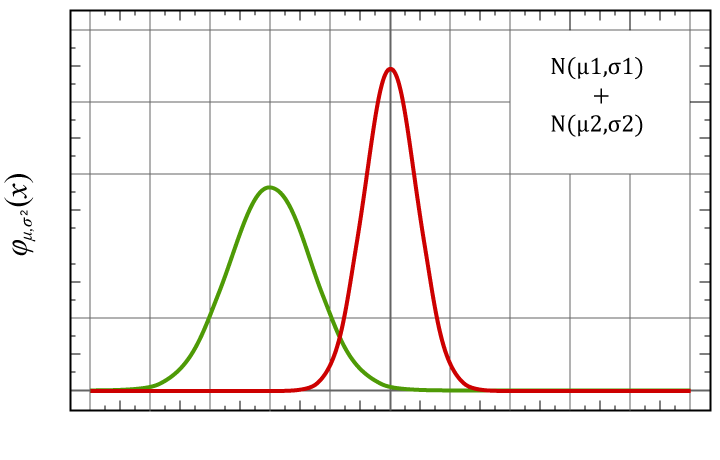
\includegraphics[width=0.7\textwidth]{img/mixture_gaussians.png}
\end{figure}

V tomto případě máme \textit{pozorovnaná data} $x_1, \dots, x_n$ a \textit{skryté proměnné} $z_1, \dots, z_n$ určující, ke které komponentě data náleží (tj. muž/žena). Lze samozřejmě sestavit model pouze na základě $X$, ten však bude poměrně složitý. Pokud přidáme skrytou proměnou $Z$, výrazně se tím model zjednoduší. Proměnná $Z$ nabývá hodnot 1 (muž) nebo 2 (žena), přičemž
$$X_i|(Z_i = 1) \sim \mathcal{N}(\mu_1,\sigma_1) \qquad\text{a}\qquad X_i|(Z_i = 2) \sim \mathcal{N}(\mu_2,\sigma_2)$$
Tedy $X_i$ se řídí rozdělením $\mathcal{N}(\mu_1,\sigma_1)$, pokud je $Z_i = 1$; a rozdělením $\mathcal{N}(\mu_2,\sigma_2)$ pokud je $Z_i = 2$. Označíme
$$P(Z_i = 1) = \tau_1 = \tau \qquad \text{a}\qquad P(Z_i = 1) = \tau_2 = (1-\tau)$$

Parametry modelu jsou tedy 
$$\theta = (\tau,\mu_1,\sigma_1,\mu_2,\mu_2)$$
a pravděpodobnostní rozložení proměnné $X$ lze vyjádřit jako
$$g_X = \tau\cdot \varphi_{\mu_1,\sigma_1} + (1 - \tau)\varphi_{\mu_2,\sigma_2}$$

kde $\varphi_{\mu,\sigma}$ je hustota pravděpodobnosti $\mathcal{N}(\mu,\sigma)$, tj. normálního rozdělení se střední hodnotou $\mu$ a odchylkou $\sigma$.

\textit{(Pozn.: Kdybychom neuvažovali $Z$ a modelovali data pomocí jediného normálního rozdělení, byly by parametry modelu pouze $\theta = (\mu,\sigma)$, které bychom mohli odhadnout jednoduše např. pomocí ML. Což by bylo jednodušší, ale hůře by to vystihovalo data.)}

Budeme chtít minimalizovat chybu modelu, tzn. maximalizovat věrohodnost modelu (resp. jeho parametrů) pro daná data. Připomenutí: \textit{pravděpodobnost (probability)} je pravděpodobnost dat na základě modelu, \textit{věrohodnost (likelihood)} je pravděpodobnost modelu (jeho parametrů) na základě dat. Platí ekvivalence
$$\mathcal{L}(\theta;X) = P(X|\theta)$$

\begin{figure}[H]
\centering
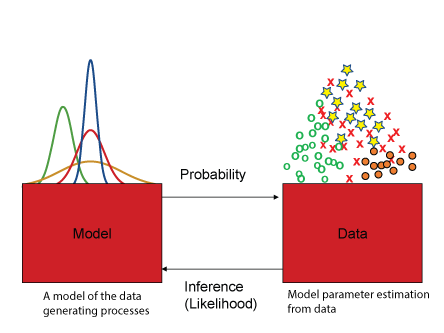
\includegraphics[scale=0.6]{img/likelihood.png}
\end{figure}

My však nemáme $P(X|\theta)$, nýbrž $P(X,Z|\theta)$ (to byl náš původní trik -- přidat proměnnou, abychom si zjednodušili model). Použijeme tedy marginální pravděpodobnosti
$$\mathcal{L}(\theta;X) = P(X|\theta) = \sum_{Z}P(X,Z|\theta)$$

V praxi se používá \textit{log-likelihood}, tj. $l(\theta;X) = \log \mathcal{L}(\theta;X) = \log P(X|\theta)$, v našem případě tedy maximalizujeme:
\begin{align*}
l(\theta;X) &= \log\sum_{Z}P(X,Z|\theta) = \sum_{i=1}^{N} \log\sum_{j=1}^{2}P(Z_i=j)\cdot\varphi_{\mu_j,\sigma_j}(x_i)\\
&=\sum_{i=1}^{N} \log[\tau\cdot \varphi_{\mu_1,\sigma_1}(x_i) + (1 - \tau)\varphi_{\mu_2,\sigma_2}(x_i)]\\
\end{align*}

Přímá maximalizace této sumy je však výpočetně náročná, proto EM používá trik: tipneme si $\theta$ (na začátku náhodně), pomocí něj odhadneme $Z$. Pomocí $X$ a odhadnutého $Z$ pak spočteme lepší odhad $\theta$.

Formálně se jedná o dva kroky
\begin{enumerate}
	\item \textbf{Expectation:} Na základě aktuálních parametrů $\theta$ a pozorovaných dat $X$ odhadni $Z$. Poté spočti \textit{očekávanou hodnotu} log-likelihood funkce (tj. váženou odhadem dané hodnoty $Z$):
	$$Q(\theta|\theta^{(t)}) = E_{Z|X,\theta^{(t)}} [\log L(\theta;X,Z)]$$
	\item \textbf{Maximization:} Najdi nové hodnoty $\theta$ maximalizující likelihood -- v tuhle chvíli \uv{známe} $Z$ (odhadnuté v předchozím kroku), takže tato maximalizace je jednoduchá:
	$$\theta^{(t+1)} = \arg\max_\theta Q(\theta|\theta^{(t)})$$
\end{enumerate}

Pro náš příklad směsi gaussovských rozdělení:
\bigskip
\begin{algorithm}[H]
	\caption{EM pro směs 2 gaussovských rozdělení}
	\begin{algorithmic}[1]
		\State $\theta = (\mu_1,\sigma_1,\mu_2,\sigma_2,\tau) \gets$ náhodná inicializace
		\While{\textbf{not} converged}
		\State \textbf{Expectation step:} Spočti
		$$\gamma_i = \frac{\tau\varphi_{\mu_1,\sigma_1(x_i)}}{\tau\varphi_{\mu_1,\sigma_1(x_i)} 
			+ (1-\tau)\varphi_{\mu_2,\sigma_2(x_i)}}$$
		\Comment{$\gamma_i$ je pravděpodobnost, že $z_i = 1$ v daném kroku, tj. pro aktuální parametry $\theta$. Máme tedy odhad $Z$, můžeme pokračovat k maximalizaci.}t
		
		\State \textbf{Maximization step:} Uprav parametry modelu $\theta$ na základě spočtených odhadů $Z$:
		$$
		\mu_1 = \frac{\sum_{i=1}^{N}\gamma_i x_i}{\sum_{i=1}^{N}\gamma_i},\qquad
		\sigma^2_1 = \frac{\sum_{i=1}^{N}\gamma_i (x_i - \mu_1)^2}{\sum_{i=1}^{N}\gamma_i}
		$$
		$$
		\mu_2 = \frac{\sum_{i=1}^{N}(1-\gamma_i) x_i}{\sum_{i=1}^{N}(1-\gamma_i)},\qquad
		\sigma^2_2 = \frac{\sum_{i=1}^{N}(1-\gamma_i)(x_i - \mu_2)^2}{\sum_{i=1}^{N}(1-\gamma_i)}
		$$
		$$\tau = \sum_{i=1}^{N}\frac{\gamma_i}{N}$$
		\EndWhile
	\end{algorithmic}
\end{algorithm}		

\bigskip
Obecně lze celý EM algoritmus zapsat jediným nesrozumitelným vzorcem:
$$\theta^{(t+1)} = \arg\max_\theta\sum_{data}\sum_{z \in Z} P(Z = z | data,\theta^{(t)}) \cdot \log P(data, Z = z |\theta)$$


\subsection{Prohledávání prostoru verzí}
\subsubsection{Znalosti v učení}
Umíme se učit funkce vstup $\to$ výstup. Jedinou dodatečnou znalost, kterou jsme využili, byl tvar hypotézy (např. lineární funkce), resp. prostor hypotéz (např. polynomiální funkce). Můžeme využít již získané znalosti o světě (background knowledge)? 

Znalosti budeme nejčastěji vyjadřovat v predikátové logice prvního řádu.
Metody:
\begin{itemize}
\item metoda nejlepší současné hypotézy
\item prostor verzí
\item induktivní logické programování
\end{itemize}

\subsubsection{Logická formulace učení}
Příklady (vzorky, data) i hypotézy budou logické formule. 
\begin{itemize}
\item \textbf{atributy} budou reprezentovány unárními predikáty (např. Alternate(X1) $\wedge$ $\lnot$Bar(X1) $\wedge$ $\lnot$Fri/Sat(X1) $\wedge$ Hungry(X1)\dots)

\item \textbf{klasifikace} vzorku (tj. cílová třída) bude také vyjádřena tzv. cílovým predikátem (např. WillWait(X1) nebo $\lnot$WillWait(X1))

\item \textbf{hypotéza} bude mít základní tvar 
$$\forall x\ Goal(x) \Leftrightarrow C_j(x)$$
kde $C_j$ je tzv. \textit{extenze hypotézy}.

Příklad: 
\begin{align*}
\forall r\ WillWait(r) &\Leftrightarrow Patrons(r,Some)\\
&\vee (Patrons(r,Full) \wedge Hungry(r) \wedge Type(r,French))\\
&\vee (Patrons(r,Full) \wedge Hungry(r) \wedge Type(r,Thai) \wedge Fri/Sat(r))\\
&\vee (Patrons(r,Full) \wedge Hungry(r) \wedge Type(r,Burger))\\
\end{align*}
\begin{figure}[H]
	\centering
	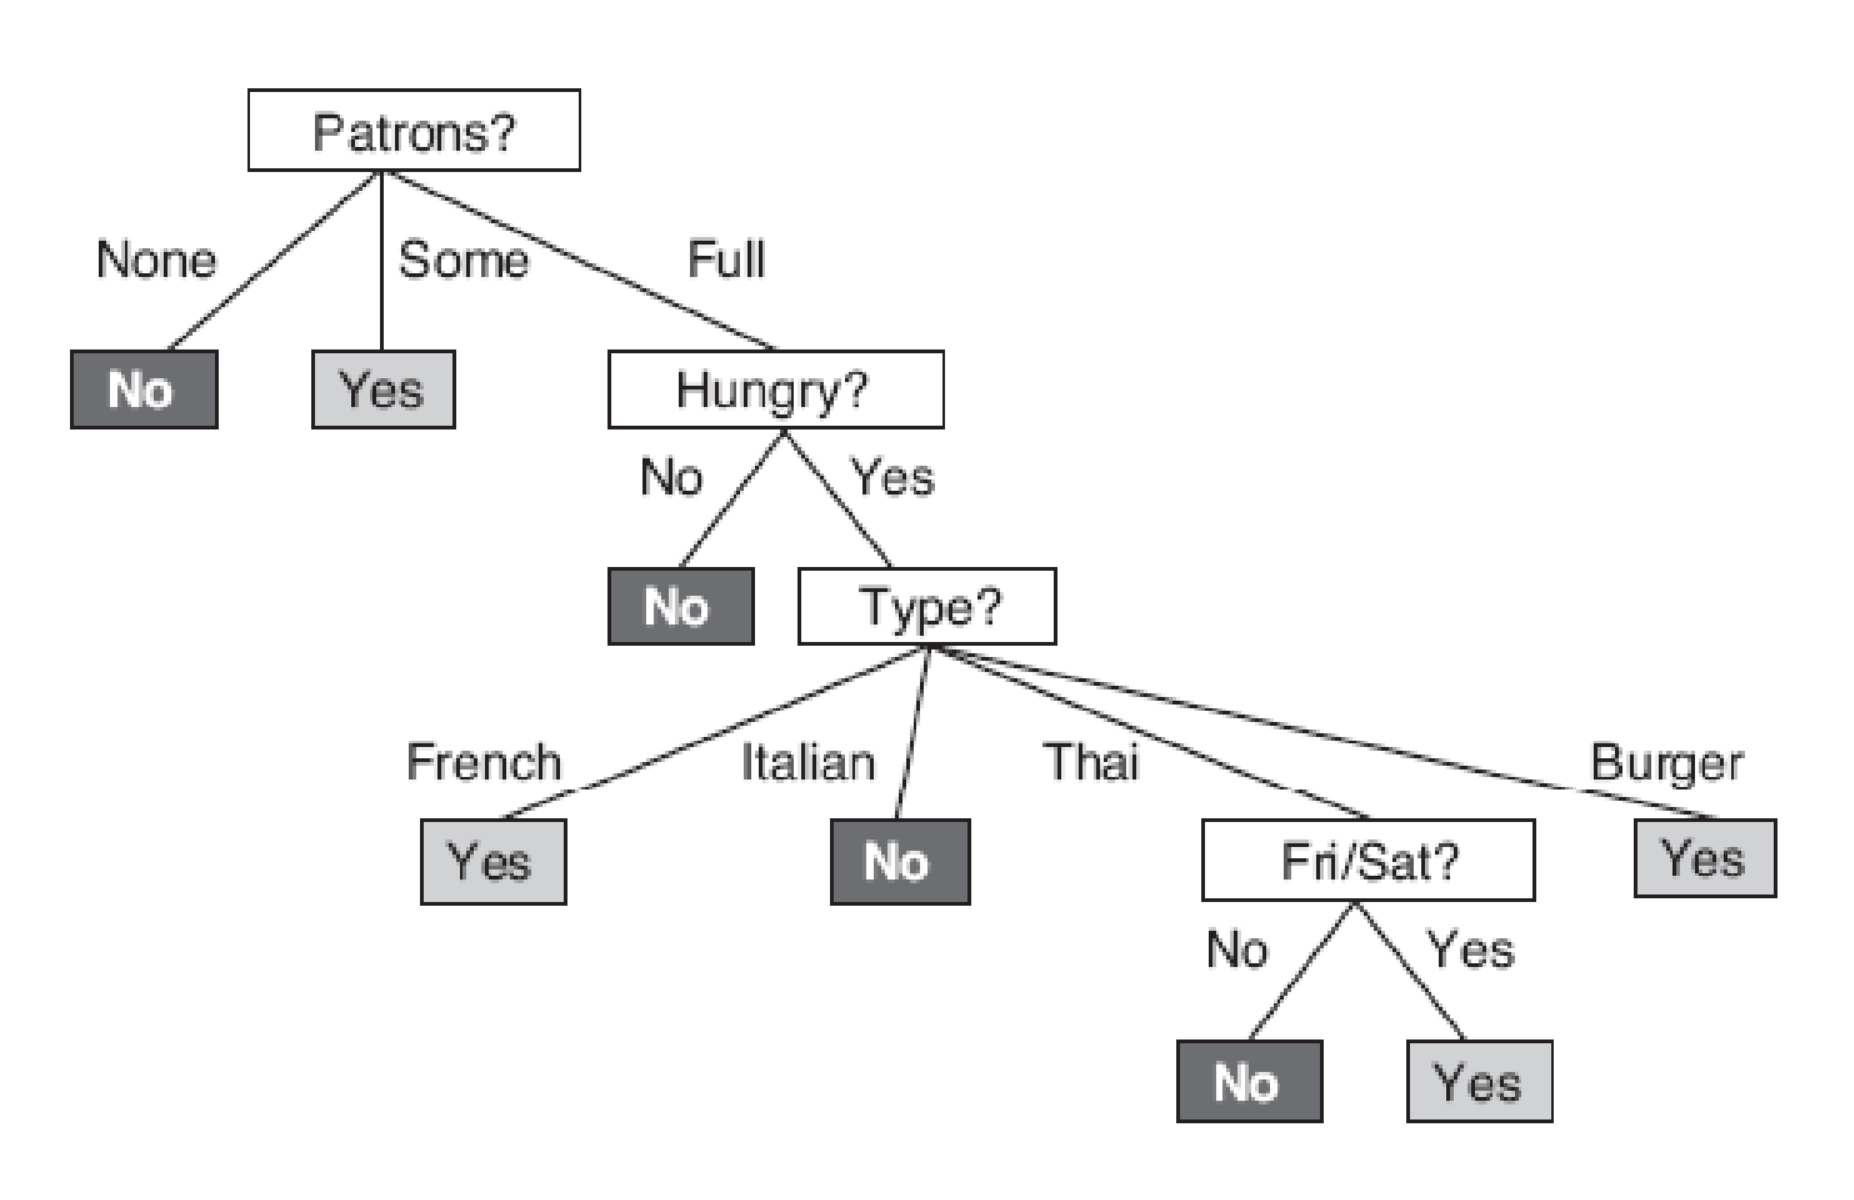
\includegraphics[scale=0.6]{img/logic_learning.png}
\end{figure}

\end{itemize}

\subsubsection{Prostor hypotéz}
\textbf{Prostor hypotéz} je množina všech hypotéz. Učící algoritmus přepokládá, že nějaká hypotéza je správná, tj. platí: $h_1 \vee h_2 \vee \dots \vee h_n$. 

Dva typy nekonzistence (pro binární klasifikaci) \textbf{falešně negativní} (hypotéza tvrdí, že příklad je negativní, ale ve skutečnosti je pozitivní) \textbf{falešně pozitivní} (naopak).

\subsubsection{Metody}
\paragraph{Metoda nejlepší současné hypotézy}
Udržujeme jednu hypotézu (current-best hypothesis) a podle příkladů ji upravujeme:
\begin{itemize}
\item příklad je s hypotézou konzistentní konzistentní $\to$ hypotézu \textbf{neměníme}
\item falešně negativní $\to$ hypotézu \textbf{zobecníme}

Pokud je hypotéza $h_1$ \textit{zobecněním} hypotézy $h_2$, potom platí $\forall x \ C_2(x) \Rightarrow C_1(x)$.

Hypotéza je typicky konjunkcí predikátů $\to$ zobecnění uděláme \textit{\uv{vypuštěním} podmínek} nebo \textit{přidáním disjunkce}.

\item falešně pozitivní $\to$ hypotézu \textbf{specializujeme}

Specializaci uděláme \textit{přidáním podmínek} nebo \textit{vypuštěním nějaké disjunkce}.
\end{itemize}


\subparagraph{Vlastnosti}
Po každé modifikaci hypotézy je potřeba \textbf{kontrolovat všechny předchozí příklady} (pouze modifikace, které jsou s nimi konzistentní, jsou povolené).

Při prohledávání často dochází k množství návratů (backtracking).

Prapůvodce problémů – příliš silný závazek: algoritmus musí v každém kroku vybrat jednu konkrétní hypotézu i když k tomu nemá dostatek informací. Řešením může být metoda nejmenších závazků.

\paragraph{Prostor verzí}
Prostor hypotéz lze reprezentovat disjunkcí $h_1 \vee h_2 \vee \dots \vee h_n$. Pokud je nějaká hypotéza nekonzistentní s příkladem, vyřadíme ji z disjunkce. Mezi zbylými hypotézami v disjunkci pořád zůstává ta správná (pokud existuje).

Obecně \textbf{prostor verzí (version space)} je množina možných hypotéz, které jsou konzistentní s dosud zpracovanými příklady.

Algoritmus \textit{eliminace kandidátů} postupně zmenšuje prostor verzí. Algoritmus je \textit{inkrementální}, tj. po přidání příkladu není potřeba kontrolovat předchozí příklady.

\subparagraph{Reprezentace}
Jak reprezentovat velkou (potenciálně nekonečnou) disjunkci? Pokud máme k dispozici uspořádání hypotéz (a to máme pomocí zobecnění/specializace), můžeme prostor verzí
reprezentovat \textit{dolní a horní mezí}.

\begin{itemize}
\item $G$ = \textbf{nejobecnější hypotézy} konzistentní s dosavadními příklady (žádná jiná konzistentní hypotéza není obecnější). Na začátku obashuje pouze $True$.

\item $S$ = \textbf{nejspecifičtější hypotézy} konzistentní s dosavadními příklady (žádná konzistentní hypotéza není specifičtější). Na začátku obsahuje pouze $False$.
\end{itemize}
\begin{figure}[H]
	\centering
	\includegraphics[width=0.45\textwidth]{img/version_space.png}
	\includegraphics[width=0.40\textwidth]{img/version_space2.png}
\end{figure}
Všechny hypotézy mezi S a G jsou konzistentní s příklady a žádné jiné konzistentní nejsou. 

Po přidání nového příkladu upravíme množiny $G$ a $S$ takto:
\begin{itemize}
\item příklad je falešně pozitivní pro $S_i$ $\to$ vyřadíme $S_i$ z množiny $S$
\item příklad je falešně negativní pro $S_i$ $\to$ nahradíme $S_i$ v množině $S$ všemi přímými zobecněními
\item příklad je falešně pozitivní pro $G_i$ $\to$ nahradíme $G_i$ v množině $G$ všemi přímými specializacemi
\item příklad je falešně negativní pro $G_i$ $\to$ vyřadíme $G_i$ z množiny $G$
\end{itemize}

Algoritmus eliminace kandidátů končí pokud:
\begin{itemize}
\item zůstala jediná hypotéza
\item rostor hypotéz zkolaboval (množina $G$ nebo $S$ je prázdná)
\item jsme vyčerpali všechny příklady. Prostor verzí potom reprezentuje disjunkci. Pokud zbylé hypotézy klasifikují různě, můžeme vybrat majoritní odpověď
\end{itemize}

\subparagraph{Vlastnosti}
Šum v datech nebo chybějící hodnoty atributů způsobují kolaps prostoru verzí. Zatím nebylo nalezeno obecně fungující řešení. 

Pokud povolíme \textit{neomezené} disjunkce, tak $S$ bude disjunkce popisů pozitivních příkladů $G$ bude negace disjunkce popisů negativních příkladů. Můžeme omezit tvar disjunkce nebo použijeme hierarchii zobecnění predikátů.

\paragraph{Induktivní logické programování (ILP)}
Kombinuje induktivní učící metody s logickou reprezentací (logickými programy). Na rozdíl od technik založených na atributech ILP umí dobře pracovat \textbf{s relacemi}.

V principu se jedná o řešení problému: hledání \textit{hypotézy} použitím známých znalostí (\textit{Background}) z příkladů popsaných \textit{Descriptions} a \textit{Classifications}, tž.
$$\text{Background} \wedge \text{Hypothesis} \wedge \text{Descriptions} |= \text{Classifications}$$

Dvě hlavní metody učení:
\begin{itemize}
\item postup shora-dolů (systém FOIL)
\item inverzní rezoluce (systém PROGOL)	
\end{itemize}

\subparagraph{ILP problém}
$$\text{Background} \wedge \text{Hypothesis} \wedge \text{Descriptions}\ {|}= \text{Classifications}$$

Příklady (\textit{Descriptions}) jsou typicky popsány Prologovskými fakty, např
\begin{itemize}
\item Father(Philip,Charles), Father(Philip, Anne), …
\item Mother(Mum,Margaret), Mother(Mum, Elizabeth), …
\item Married(Diana, Charles), Married(Elizabeth, Philip), …
\item Male(Philip), Male(Charles), …
\item Female(Beatrice), Female(Margaret),…
\end{itemize}

Podobně známá klasifikace (\textit{Classification}) je dána fakty:
\begin{itemize}
\item Grandparent(Mum,Charles), Gradparent(Elizabeth, Beatrice), …
\item $\lnot$Gradparent(Mum,Harry), $\lnot$Grandparent(Spencer,Peter), …
\end{itemize}

Možná hypotéza (\textit{Hypothesis}):
\begin{align*}
Grandparent(x,y) &\Leftrightarrow [\exists z\ Mother(x,z) \wedge Mother(z,y)]\\
&[\exists z Mother(x,z) \wedge Father(z,y)] \\
&[\exists z Father(x,z) \wedge Mother(z,y)] \\
&[\exists z Father(x,z) \wedge Father(z,y)] \\
\end{align*}

Použijeme-li znalost (\textit{Background})
$$Parent(x,y) \Leftrightarrow Mother(x,y) \vee Father(x,y)$$

potom můžeme hypotézu zjednodušit:
$$Grandparent(x,y) \Leftrightarrow [\exists z\ Parent(x,z) \wedge Parent(z,y)]$$

\subparagraph{Metoda shora-dolů}
Začneme klauzulí s prázdným tělem
$$Grandfather(x,y) \gets $$

Klasifikuje všechny příklady jako pozitivní, takže ji postupně budeme specializovat
přidáním literálu do těla klauzule
\begin{align*}
Grandfather(x,y) \gets Father(x,y) \\
Grandfather(x,y) \gets Parent(x,z) \\
Grandfather(x,y) \gets Father(x,z) \\
\dots \\
\end{align*}
Vybereme tu specializaci, která klasifikuje nejvíce pozitivních a negativních příkladů.

Pokračujeme ve specializaci
$$Grandfather(x,y) \gets Father(x,z) \wedge Parent(z,y)$$

pokud nemáme k dispozici znalost $Parent$, můžeme získat více klauzulí
\begin{align*}
Grandfather(x,y) \gets Father(x,z) \wedge Father(z,y) \\
Grandfather(x,y) \gets Father(x,z) \wedge Mother(z,y) \\
\end{align*}
Každá klauzule pokrývá některé pozitivní příklady a žádný negativní příklad.

Literály se vybírají ze známých predikátů, rovnosti/nerovnosti a aritmetických porovnání. Musí obsahovat proměnnou, která už v klauzuli je. Můžeme použít znalost typů (číslo, osoba,\dots). Volba literálu se dělá na základě \textit{informačního zisku}.

\subparagraph{Inverzní rezoluce}
$$\text{Background} \wedge \text{Hypothesis} \wedge \text{Descriptions}\ {|}= \text{Classifications}$$

Obecná rezoluce tedy musí dokázat Classifications z Background, Hypothesis, Descriptions. Můžeme jít v rezoluci obráceně a hledat Hypothesis, kterou k důkazu potřebujeme, tj. z rezolventy C hledáme C1 a C2 (máme-li C2, hledáme jen C1).


\section{Evoluční algoritmy; základní pojmy a teoretické poznatky, hypotéza o stavebních blocích, koevoluce, aplikace evolučních algoritmů.}
Skip.

\section{Strojové učení v počítačové lingvistice a algoritmy pro statistický parsing.}
Od 80. a 90. let se ve \textbf{zpracování přirozených jazyků (NLP, Natural Language Processing)} začaly silně uplatňovat metody strojového učení. Dříve se při úkolech spojených se zpracováním jazyků spoléhalo na ručně zakódovaná pravidla. Ta se nyní získávají pomocí \textbf{statistické inference} z velkých korpusů textů, ideálně získaných z reálných zdrojů (tj. ne umělé). 

Mnoho metod strojového učení již bylo adaptováno pro NLP. Rozhodovací stromy generují systém rozhodovacích if-then pravidel, na která byla tehdy komunita zvyklá. Postupně se však na výsluní dostaly \textbf{statistické modely}, které pracují s pravděpodobnostmi, váhami na vstupních příznacích a s mírou nejistoty.

Využití metod strojového učení má mnoho výhod:
\begin{itemize}
	
	
	\item Statistické učení se automaticky zaměřuje na \textbf{nejčastější} (a tedy důležité) případy.
	\item Budované modely jsou typicky \textbf{robustní} vůči novým \textbf{neznámémým datům} a \textbf{zašuměnému či chybnému vstupu}. Toho je u ručně psaných pravidel velmi obtížné dosáhnout.
	\item Modely lze zpřesňovat poskytnutím dodatečných trénovacích dat. U ručně psaných pravidel to lze pouze zvyšováním komplexity modelu.
\end{itemize}

Strojové učení a NLP se vlastně dobře doplňují. NLP samotné nedokáže text zpracovat o moc lépe, než jako \uv{bag-of-words}, kdežto NLP má prostředky pro extrakci struktury (morfologie, syntax, sémantika) z textu. Naopak NLP nedokáže s těchto poznatků získat nějakou hlubší informaci, kdežto strojové učení na to má spoustu nástrojů. Nabízí se tedy výhodná spolupráce: NLP extrahuje sofistikované informace o struktuře, které pak strojové učení použije jako příznaky pro učení nějakého modelu.

\hrule
\medskip
\textit{Následující sekce jsou výtahem z přednášek NPFL067 a NPFL068}
\subsection{Základy teorie informace}
Nechť $p_X{x}$ je pravděpodobnostní rozdělení náhodné proměnné $X$ a nechť $\Omega$ je množina základních jevů. Pak \textbf{entropie} tohoto rozdělení je 
$$H(X) = -\sum\limits_{x \in \Omega} p(x) \cdot \log_2(p(x))$$
Entropie vyjadřuje \textit{míru nejistoty}. Vyjadřuje se v bitech. Nejnižší možná hodnota je 0 (pokud je výsledek experimentu dán předem), horní limit obecně není -- nicméně největší nejistota odpovídá uniformnímu rozdělení, tj. pro $|\Omega| = n : H(X) \leq \log_2 (n)$. Entropii lze taktéž interpretovat jako minimální počet bitů nutných pro zakódování nějaké informace: čím předvídatelnějí jsou data, tím úspornější kódování.

\textbf{Podmíněnou entropii} náhodných proměnných $X$ (prostor $\Omega$) a $Y$ (prostor $\Psi$) definujeme jako:
$$H(Y|X) = -\sum\limits_{x \in \Omega} \sum\limits_{y \in \Psi} p(x,y) \cdot \log_2 p(y|x)$$ 
Důležité: první pravděpodobnost \textbf{není} podmíněná! Jedná se z jistého pohledu o vážený průměr, kde $p(x,y)$ je váha a ta není podmíněná.

Podmíněná entropie je vždy lepší, tj. $H(Y|X) \leq H(Y)$. Tedy vždy se nám hodí mít nějakou znalost podmiňující odhadovanou proměnnou (příklad: chceme-li odhadnout další slovo ve větě, náš odhad jistě zlepší znalost slovníku daného jazyka včetně distribuce slov).

Abychom změřili, nakolik naše znalost $X$ pomůže odhadu $Y$, můžeme použít míru \textbf{vzájemné informace (MI, Mutual Information)}:
$$I(X,Y) = \sum\limits_{x \in \Omega} \sum\limits_{y \in \Psi} p(x,y) \cdot \log_2 \frac{p(x,y)}{p(x)p(y)}$$ 
Ta se měří rovněž v bitech. Vyjadřuje, o kolik bitů znalost $X$ sníží entropii $Y$.

Posledním důležitým nástrojem z teorie informace je \textbf{cross-entropie}. Ta vyjadřuje, nakolik naše pozorování odpovídají očekávanému pravděpodobnostnímu rozdělení. Nechť $p$ označuje očekávané rozdělení (získané například analýzou slovníku) a $p'$ označuje odhad pravděpodobností na základě pozorovaných dat (typicky $p'(x) = $počet pozorování $x$ děleno celkový počet pozorování):
$$H_p(p') = -\sum\limits_{x \in \Omega} p(x) \cdot \log_2(p'(x))$$
Cross-entropie slouží nikoliv k ohodnocení či porovnání pozorovaných dat, ale k \textbf{porovnání různých distribucí}. Máme-li dvě distribuce $p$ a $q$, pak porovnáním jejich cross-entropií na reálných datech (tj. $H_p(p')$ vs. $H_q(p')$) zjistíme, které z nich lépe vystihuje reálná data -- tj. má nižší cross-entropii (např. máme 2 slovníky pro nějaký jazyk včetně pravděpodobností výskytů jednotlivých slov; na základě reálného vzorku nějakého textu můžeme rozhodnout, který slovník jej odhaduje lépe).

I cross-entropie může být \textbf{podmíněná}:
$$H_p(p') = -\sum\limits_{x \in \Omega} \sum\limits_{y \in \Psi} p(x,y) \cdot \log_2 p'(y|x)$$ 
Často se vyplácí sčítat nikoliv přes celý prostor jevů, ale pouze přes \textbf{slovníková data $T$}:
$$H_p(p') = -\frac{1}{|T|}\sum\limits_{i = 1 \dots |T|}\log_2 p'(y_i|x_i)$$ 

\subsection{Modelování jazyka, zašuměný kanál}
\textbf{Zašuměný kanál} je označení pro modela média, které k přenášeným slovům přidá nějaký šum. Formálně: do kanálu vstupuje nějaká sekvence symbolů, z něj pak vystupuje pozměněná, zašuměná sekvence, kterou my přijmeme. Cílem je tedy na základě přijaté zašuměné sekvence uhodnout původní zprávu.

\begin{figure}[H]
	\centering
	\includegraphics[]{img/noisy_channel.png}
\end{figure}

Mnoho problémů NLP lze chápat jako případ zašuměného kanálu, např. rozpoznávání mluvené řeči, OCR, strojový překlad (\uv{šum} kvůli překladu), \dots

Formálně nás tedy zajímá podmíněná pravděpodobnost původní zprávy $A$ za předpokladu přijaté zprávy $B$, tedy $p(A|B)$. Díky Bayesově větě:
$$p(A|B) = p(B|A)p(A)/p(B)$$
Zajímá nás nejpravděpodobnější možnost, tj.
$$A_best = \text{argmax}_A p(B|A)p(A)/p(B) =\text{argmax}_A p(B|A)p(A)$$
kde $p(B)$ lze ignorovat, protože je pro všechny možnosti $A$ stejné. Náš výpočet má tedy nyní dvě složky:
\begin{itemize}
	
	
	\item $p(B|A)$: akustický/překladový/\dots model (záleží na konkrétním problému)
	\item $p(A)$: \textbf{jazykový model}
\end{itemize}
 
Z hlediska ručně kódovaných pravidel je přirozeným popisem jazyka nějaká \textit{gramatika}. Z hlediska statistického zpracování je základem statistický \textbf{jazykový model} (LM, Language Model). Ten tvoří \textbf{pravděpodobnostní distribuce přes sekvence slov}, tj. každé sekvenci $W = (w_1, w_2, \dots w_k)$ přiřadí pravděpodobnost $p(W) = p(w_1,w_2,\dots w_k)$. To můžeme jednoduše přeformulovat díky Bayesovu pravidlu a řetízkovému pravidlu na 
$$p(W) = p(w_1,w_2,\dots w_k) = p(w_1) \times p(w_2|w_1) \times p(w_3|w_1,w_2) \times \dots \times p(w_k|w_1,w_2,\dots,w_{k-1})$$

Tato přímočará formulace je ale nepraktická kvůli vysokému počtu parametrů i pro relativně krátká $W$. Nejčastější v praxi používanou variantou je tzv. \textbf{n-gram Language Model}, kdy je \uv{paměť} omezena na posledních $n$ slov, tj.
$$p(W) = p(w_1,w_2,\dots w_k) = \prod\limits_{i = 1}^{k} p(w_i|w_{i-n+1}, w_{n-n+2},\dots,w_{i-1})$$
Pro každé slovo tedy spočteme jeho pravděpodobnost za \textbf{předpokladu předchozích $n$ slov}, celková pravděpodobnost sekvence je pak \textbf{součinem pravděpodobností jednotlivých slov}.

Příklady pro malá $n$:
\begin{description}
	
	
	\item[0-gram LM: uniformní model] 	\quad $p(w) = \frac{1}{|V|}$  (pro slovník velikosti $|V|$)
	\item[1-gram LM: unigram model] 	\quad $p(w)$
	\item[2-gram LM: bigram model] 		\quad $p(w_i|w_{i-1})$
	\item[3-gram LM: trigram model] 	\quad $p(w_i|w_{i-2},w_{i-1})$
\end{description}

Čím vyšší $n$, tím přesnější model, nicméně za cenu nárůstu složitosti. Používá se $n = 3$ (\textbf{trigram model}). 

Tento model odpovídá \textbf{Markovovu procesu (řetězci)} řádu $n-1$. Markovův řetězec (1. řádu) je jakákoliv posloupnost (stavů, hodnot, \dots), která splňuje 2 vlastnosti:
\begin{enumerate}
	
	
	\item \textbf{omezená historie:} $\forall i \in 1\dots T : P(X_i|X_1,X_2,\dots X_{i-1}) = P(X_i|X_{i-1})$
	Tj. aktuální hodnota je podmíněna pouze předchozí hodnotou.
	\item \textbf{stacionarita:} $\forall i \in 1\dots T, \forall x,y \in S : P(X_i = x | Y_i = y) = p(x|y)$ 
	Tj. pravděpodobnost přechodu z $x$ do $y$ je stejná nezávisle na pozici v sekvenci.
\end{enumerate}
Díky stacionaritě se Markovovy řetězce jednoduše reprezentují pomocí \textit{stavových diagramů}. Definici lze také jednoduše rozšířit na vyšší řády. Pak jsou stavy v diagramu odpovídající $n$-tice.

Jazykový model se získává z trénovacích dat (preprocessing: sjednocení velikosti písmen, anotace konců vět, \dots), a to strategií \textbf{Maximum Likelihood Estimate (MLE)} (maximálně věrohodný odhad), který je založen na počtech výskytů jednotlivých n-gramů v trénovacích datech. Trigramový model pak získáme jako
$$p(w_i|w_{i-2},w_{i-1}) = \frac{c_3(w_{i-2}, w_{i-1}, w_{i})}{c_2(w_{i-1}, w_{i})}$$
kde $c_2$ resp. $c_3$ označuje počet výskytů daného bigramu resp. trigramu v trénovacích datech. Tato metoda nefunguje na začátku trénovacích dat, pro se často přidávají 2 \uv{dummy} slova před začátek trénovacích dat. 

\subsection{Vyhlazování jazykového modelu}
Problémem popsaného modelu jsou nulové pravděpodobnosti $n$-gramů, které se v trénovacích datech vůbec nevyskytují. To je samozřejmě nežádoucí (na nových datech pak může vyjít nekonečná cross-entropie) a řeší se to tzv. \textbf{vyhlazováním} (angl. \textit{LM smoothing}). Existuje více strategií, ale obecná idea je stejná: ubrat nějakým nenulovým $p(w)$ a distribuovat mezi nulové $p(w)$, čímž získáme nové, vyhlazené rozdělení $p'(w)$. Vždy však musíme dbát na to, aby součet pravděpodobností byl 1.

Strategie:
\begin{description}
	
	
	\item[přidání jedničky:] K počtu výskytů každého ze všech \textit{možných} slov ze slovníku $V$ přičteme jedničku:
	$$p'(w) = \frac{c(w) + 1}{|T| + |V|}$$
	kde $T$ je trénovací množina (a původní výpočet by tedy vypadal $p(w) = c(w)/|T|$)
	
	V případě $n$-gramů pro $n > 1$ vypadá vzorec takto: $p'(w) = \frac{c(h,w) + 1}{c(h) + |V|}$, kde $h$ označuje \uv{historii}, tj. předchozích $n$ slov.
	
	Jednoduché, ale v praxi nepříliš použitelné.
	
	\item[přidání $\lambda < 1$:] Tentýž princip, pouze místo 1 přidáváme nějakou menší konstantu. Myšlenkou je opravit ten nedostatek, že přidání byť jen 1 výskytu může pro malá trénovací data velmi silně pokřivit rozdělení.
	
	$$p'(w) = \frac{c(w) + \lambda}{|T| + \lambda|V|} \quad \text{resp.} \quad p'(w) = \frac{c(h,w) + \lambda}{c(h) + \lambda|V|}$$
	
	\item[Good-Turingovo vyhlazování:] 
	$$p'(w) = \frac{(c(w)+1) \cdot N(c(w) + 1)}{|T| \cdot N(c(w))}$$
	kde $N(c)$ je počet slov s počtem výskytů rovným $c$ (\uv{počet počtů}). Speciálně pro $c(w) = 0$ je $p'(w) = \frac{N(1)}{|T|\cdot N(0)}$. Tedy pro slova s nulovým výskytem si \uv{vypůjčíme} od slov s 1 výskytem. Pro vyšší hodnoty se pak \uv{masa pravděpodobnosti} rozdistribuuje vždy směrem k \uv{potřebnějším}.
	
	\item[lineární interpolace:] \textit{Pozorování:} čím nižší řád $n$-gramů, tím méně detailní distribuce a pro $0$-gramy dokonce dostáváme uniformní rozdělení. To má sice nízkou informaci, ale na druhou stranu nemá problém s nulovými hodnotami. 
	
	\textit{Idea:} zkombinovat různé řády $n$-gramů:
	$$p'(w_i|w_{i-2}, w_{i-1}) = \lambda_3 p_3(w_i|w_{i-2}, w_{i-1}) + \lambda_2 p_2(w_{i}| w_{i-1}) + \lambda_1 p_1(w_i) + \lambda_0 \frac{1}{|V|}$$
	kde $\lambda = (\lambda_0, \lambda_1, \lambda_2, \lambda_3)$ jsou parametry ovlivňující detailnost vs. vyhlazenost výsledné distribuce. Platí $\forall i \lambda_1 > 0, \sum_i \lambda_i = 1$. Tyto parametry se odhadnou EM algoritmem (detaily vynecháme) pomocí speciálně vyčleněného datesetu (\textit{heldout data}), na němž se budeme snažit minimalizovat cross-entropii pro fixní $p_1, p_2, p_3$. Je nutné použít jiná data, než trénovací (ze kterých jsme získali $p_1, p_2, p_3$), jinak by došlo k degeneraci modelu k $\lambda = (0,0,0,1)$. Obecně se v NLP rozdělují dostupná data na 3 části: \textit{trénovací, testovací} a \textit{heldout data}.
	%TODO EM smoothing algoritmus
	
\end{description}

\subsection{Třídy slov}
Další strategií pro korekci chyby distribuce $p(w)$ způsobené příliš malým trénovacím datasetem (který nikdy nebude dost velký :)) je užití \textbf{slovních tříd}. 

Uvažme následující situaci: v trénovacích datech se setkáváme s frázemi \textit{short homework}, \textit{simple homework}, \textit{short assignment}; ale nikoliv se \textit{simple assignment}. Pak tedy $p(homework|simple)$ je vysoká, ale $p(assignment|simple)$ je velmi malá (není nulová vlastně jen díky vyhlazování). 

Pokud však seskupíme slova s podobným významem do společné třídy, tj. \textit{(simple, short)(homework, assignment)}, můžeme náš $n$-gramový model vybudovat na úrovni tříd a tím dosáhnout lepšího odhadu pro $n$-gramy, s nimiž jsme se nesetkali, ale které významově dávají smysl. Cenou za práci na úrovni tříd namísto slov je jistá ztráta informace.

Nová podoba $n$-gramového jazykového modelu je tedy následující:
$$p_n(w_i|h_i) = \frac{p(w_i|c_i)}{p_n(c_i|h_i)}$$
kde $c_i$ označuje \textbf{třídu} slova $w_i$, $p(w_i|c_i)$ popisuje pravděpodobnostní distribuci slov v této třídě a $h_i$ je historie slova $w_i$, avšak tentokrát jako \textbf{předchozích $n$ tříd} (resp. \textbf{třídy předchozích $n$ slov})! Např. pro trigramový model je $h_i = c_{i-2},c_{i-1}$, nikoliv $w_{i-2},w_{i-1}$!

I pro třídy lze použít lineárně vyhlazený model.

Rozdělení slov do tříd můžeme získat třeba z nějakého slovníku, nicméně jak je ve strojovém učení zvykem, raději ho sestrojíme z dostupných dat. Algoritmus je následující:

Nechť $V$ je množina slov (=slovník), $C$ je množina tříd a $r : V \mapsto C$ je mapování slov do do tříd.
\begin{enumerate}
	
	
	\item Na začátku je každé slovo ve vlastní třídě, tj. $V = C, r = \text{id}$
	\item Vyber dvě třídy $k,j$ takové, že
	$$(k,l) = \text{argmax}_{k,l} I_{merge(r,k,l)}(D,E)$$
	kde $I(D,E)$ vyjadřuje \textit{vzájemnou informaci} pro sousední třídy, tj. $D,E$ jsou náhodné proměnné takové, že $d \in D, e \in E$ jsou třídy z $C$, které se v trénovacích datech vyskytují vedle sebe. $I_{merge(r,k,l)}(D,E)$ vyjadřuje tuto hodnotu po hypotetickém sloučení tříd $k,l$.
	\item sluč třídy $k,l$, přitom uprav $C$ a $r$
	\item opakuj kroky 2 a 3 dokud $|C|$ nedosáhne předem dané velikosti
\end{enumerate}

Pozor, $k,l$ typicky nejsou sousední třídy, kterých se týká $I(D,E)$! Optimálně to jsou třídy slov, která se vyskytují v podobném kontextu a proto jejich sloučení zhorší globální $I(D,E)$ co nejméně. Optimální $I(D,E)$ samozřejmě nastává v případě, že je každé slovo ve vlastní třídě, proto je důležité slučování vynucovat v každém kroku.

Důležitá je podmínka na ukončení při dosažení určitého počtu tříd (jinak bychom se dostali na jedinou třídu). 

Pro sestrojení tříd se používají \textit{trénovací} data. 

\subsection{Markovovy modely}
O jednoduchých Markovových procesech jsme se již zmínili u $n$-gramového jazykového modelu. Nyní definujeme složitější model, který se používá hned v několika odvětvích NLP.

\textbf{Skrytý Markovův model (HMM, Hidden Markov Model)} je pětice $(S, s_0, Y, P_S, P_Y)$, kde
\begin{itemize}
	
	
	\item $S = \{s_0, s_1, \dots s_T\}$ je \textbf{množina stavů}
	\item $s_0$ je \textbf{počáteční stav}
	\item $Y = \{y_1,y_2,\dots y_V\}$ je \textbf{výstupní abeceda}
	\item $P_S(s_j|s_i)$ jsou \textbf{pravděpodobností přechodu} mezi stavy. Velikost $|P_S| = |S|^2$
	\item $P_Y(y_k|s_i,s_j)$ jsou \textbf{výstupní pravděpodobnostni}. Velikost $|P_Y| = |S|^2 \times |Y|$
\end{itemize}
Výstup se v této nejobecnější verzi generuje \textit{na přechodových hranách}, časté je ale také generování výstupu ze stavů. Výstupní pravděpodobnosti udávají pro každou hranu pravděpodobnost emise daného symbolu.
\begin{figure}[H]
	\centering
	\includegraphics[scale=1]{img/hmm.png}
\end{figure}

\medskip
\textbf{Úkoly pro HMM}
\begin{itemize}
	
	
	\item\textbf{Generuj výstup. (Nepříliš hodnotné\dots)} 
	
	Začni v $s_0$, pohybuj se náhodně podle $P_S$, vypisuj náhodně podle $P_Y$, opakuj dokud tě někdo nezastaví.
	
	\item \textbf{Dána sekvence $Y = y_1y_2\dots y_k$, spočti její pravděpodobnost.}\footnote{Občas nesprávně označován jako Trellisův algoritmus, ale \uv{trellis} je pouze označení jistého typu grafu, kde jsou vrcholy rozděleny do sloupců odpovídajících časům $t, t+1,\dots$}
	
	Udržujeme si \textit{trellis stavy}, tj. stav automatu v čase $t$, každý stav drží proměnnou $\alpha$. Pravděpodobnost $Y$ je pak dána jako $\sum\alpha$ předchozích stavů.
	\begin{enumerate}
		
		
		\item iniciální trellis sloupec $t_0$: obsahuje jenom $s_0$, nastav $\alpha(s_0, 0) = 1$
		\item na základě sloupce $t_{i-1}$ a aktuálního vstupního symbolu $y_i$ vytvoř následující sloupec trellis grafu, ale vyber pouze stavy, do nichž se dá dostat z aktuálního sloupce a které generují $y_1$ (resp. takové, že přechodová hrana generuje $y_1$)
		\item nastav $\alpha(state,i) = \sum\limits_{s \in t_{i-1}, \exists\text{hrana }s\rightarrow state} P_S(state|s) \cdot \alpha(s, i-1) \cdot P_Y(y_i|s,state)$
		\item jakmile $i = |Y|$ (vstup je vyčerpán), nastav $P(Y) = \sum\limits_{s \in t_{|Y|}} \alpha(s,|Y|)$	
	\end{enumerate}
	
	\begin{figure}[H]
		\centering
		\includegraphics[scale=1]{img/trellis.png}
		\captionsetup{width=0.6\textwidth}
		\caption{Příklad \uv{trellis} grafu pro vstup $Y =$ \uv{toe} (varianta s \textit{deterministickými} výstupy z \textit{vrcholů})}
	\end{figure}
	
	
	
	\item \textbf{Dána sekvence $Y = y_1y_2\dots y_k$, spočti nejpravděpodobnější posloupnost stavů, která ji vygenerovala (popř. $n$ nejpravděpodobnějších posloupností).}
	
	Požívá se \textbf{Viterbiho algoritmus}. Princip je podobný jako v předchozím úkolu, pouze v průchodu trellis grafem nebereme součet $\alpha$ pro různé hrany vedoucí do téhož vrcholu, nýbrž \textbf{bereme pouze přechod s maximální $\alpha$ hodnotou}. Současně si pamatujeme zpětné hrany, abychom na konci mohli cestu zrekonstruovat.
		
	Ve třetím kroku původního algoritmu bychom tedy použili výpočet  $$\alpha(state,i) = \max\limits_{s \in t_{i-1}, \exists\text{hrana }s\rightarrow state} (P_S(state|s) \cdot \alpha(s, i-1) \cdot P_Y(y_i|s,state))$$
	
	Pokud chceme $n$ nejlepších cest, budeme si vždy pamatovat $n$ nejlepších zpětných ukazatelů a cesty poté zrekonstruujeme pomocí backtracking algoritmu.
	
	\begin{figure}[H]
		\centering
		\includegraphics[scale=1]{img/viterbi.png}
		\caption{Příklad výpočtu Viterbiho algoritmu.}
	\end{figure}


	\item \textbf{Dána trénovací data $Y$, odhadni (tj. nauč se) parametry HMM (tj. $P_S$ a $P_Y$).}
	
	\textbf{Baum-Welch algoritmus.} Založen na EM. %TODO baum-welch
	
\end{itemize}


\subsection{Tagging}
\textbf{Tagování} je proces, kdy se snažíme slovo rozložit na \textit{lemma} (=základní tvar slova) a \textbf{tag}, tj. \uv{slovníkovou značku}, která obsahuje mluvnické kategorie, jako například číslo, pád, rod, druh, čas apod. Různé korpusy a treebanky používají různé formáty, české jsou výrazně složitější.

\begin{figure}[H]
	\centering
	\includegraphics[scale = 1]{img/czechtag.png}
	\caption{Ukázka standardní české 15-písmenné značky (tagu) včetně vysvětlivek}
\end{figure}

Formálně je tagování zobrazení $A^+ \rightarrow T$, kde $A$ je abeceda fonémů a $T$ je množina tagů, tzv. \textbf{tagset}. S tagování úzce souvisí \textit{morfologická analýza}, což je formálně zobrazení $A^+ \rightarrow 2^{L, C_1, C_2, \dots C_n}$, kde $L$ je lemma a $C_i$ jsou mluvnické kategorie. Morfologická analýza tedy přiřadí neprázdné sekvenci fonémů (=slovu) množinu možných lemmat spolu s mluvnickými kategoriemi (např. pro slovo \uv{kolem} nalezne morfologická analýza několik možností). Tagování lze pak chápat jako \textit{disambiguation}, tj. výběr jedné z možností (typicky na základě kontextu). Tag $t \in T$ je pak typicky přímo množina mluvnických kategorií $t = C_1C_2\dots C_m$.

Různé přístupy k tagování:
\begin{enumerate}
	\item \textbf{ručně psaná pravidla} Mějme následující výstup z morfologické analýzy (Penn tagset):
	\begin{figure}[H]
		\centering
		\includegraphics[scale=1]{img/tag1.png}
	\end{figure}
	Cílem je vybrat správnou sekvenci značek. Používáme \textbf{předdefinovaná pravidla if-then}, například:
		\begin{align*}
			&\text{if }(t_{i-1} = DT)\text{ then }(t_i = NN)\\
			&\text{if }((t_{i-1} = PRP) \wedge (t_{i+1} = DT))\text{ then }(t_i = NN)\\
			&\text{if }((t_{i} \in \{DT,NN\})\text{ then }(t_i = DT)\\
			&\text{if }((t_{i+1} \in \{VB,VBZ,VBP,VBD,VBG\})\text{ then }(t_i \neq DT)\\
			&\dots
		\end{align*}
	Pro každé pravidlo sestrojíme vlastní \textbf{konečný automat}, který se po skončení výpočtu nachází v přijímacím stavu, právě tehdy, pokud není pravidlo porušeno. Automaty spouštíme paralelně a zkoušíme všechny možné sekvence tagů. Pokud všechny přijímají, jde o validní otagování.
	\begin{figure}[H]
		\centering
		\includegraphics[scale=1]{img/tag_automat.png}
	\end{figure}
	
	
	\item \textbf{statistické metody}
	\begin{enumerate}
		\item \uv{pravděpodobnostní}
		\begin{enumerate}
			\item HMM
			\item maximum entropy
		\end{enumerate}
		\item pravidlové
		\begin{enumerate}
			\item TBEDL
			\item Example based
		\end{enumerate}
		\item feature-based
		\item kombinace klasifikátorů
	\end{enumerate}
\end{enumerate}



\subsection{Statistický parsing}
\textbf{Parsing (parsování)} je označení pro proces, kdy je pro vstupní větu, o níž předpokládáme, že byla vytvořena nějakou gramatikou, nalezena posloupnost pravidel této gramatiky, kterou byla věta nejpravděpodobněji vytvořena. Typicky se pro větou rovnou sestrojí \textit{parsovací strom}.


\subsection{Statistický strojový překlad}
Klasickým přístupem je chápat strojový překlad jako problém \textbf{zašuměného kanálu}, kdy například při překladu z francouzštiny do angličtiny je nezkresleným vstupem anglická věta $E$ a \uv{zašuměným výstupem} je francouzská věta $F$. Naším cílem je pak nalézt nejpravděpodobnější původní řetězec, tj. nejpravděpodobnější překlad do EN. Formálně $P(E|F) = P(F|E)\cdot P(E) / P(F)$, nejpravděpodobnější překlad je 
$$\text{argmax}_E = \text{argmax}_E P(E|F) = P(F|E)\cdot P(E)$$
Opět vynecháme člen $P(F)$, jelikož ten je pro všechna $E$ stejný.

Potřebujeme tedy \textbf{language model (LM)} $P(E)$, \textbf{translation model (TM)} $P(F|E)$ a vyhledávací proceduru, která k $E$ nalezne nejlepší $F$ pomocí LM a TM. 
\begin{description}
	\item[Language Model] Lze použít v podstatě jakýkoliv, např. (smoothed) 3-gram LM, 3-gram s třídami, \dots Jazykový model nemusí nutně operovat přímo se slovy/slovními tvary, může se hodit přidat úroveň abstrakce (viz níže).
	
	\item[Translation Model] Nestará se o korektnost anglických vět, to je starost LM. To nám dává větší volnost.
	
	Typicky nemáme mapování 1:1, věty bývají i jinak dlouhé. Proto se používá \textbf{Alignment (zarovnání)}:
	
	\begin{figure}[H]
		\centering
		\includegraphics[scale = 1]{img/translation_alignment.png}
	\end{figure}

	Označíme $m = |F|, l = |E|$, pak máme celkem $m\cdot l$ možných spojů mezi větami $E$ a $F$; jedno konkrétní zarovnání je pak nějaká podmnožina těchto spojů, tj. celkem $2^{ml}$ různých zarovnání. V praxi to však bývá o něco lepší, např. při překladu EN $\rightarrow$ FR má každé anglické slovo $1\dots n$ spojů a každé francouzské \textit{právě} jeden spoj. To je tedy celkem \uv{pouze} $(1+l)^m$ zarovnání.
	
	Nechť celková pravděpodobnost anglické věty $E$, francouzské věty $F$ a zarovnání $A$ je $P(F,A,E)$. Pak můžeme vyjádřit $P(F|E)$ jako
	$$P(F|E) = \frac{P(F,E)}{P(E)} = \frac{\sum_A P(F,A,E)}{\sum_{A,F} P(F,A,E)} = \sum_A P(F,A |E) $$
	
	Jedna z možných \textbf{dekompozic} pravděpodobnosti $P(F,A|E)$, kterou budeme používat, je tato:
	$$P(F,A|E) = P(m|E) \cdot \prod\limits_{j=1}^{m} P(a_j | a_l^{j-1}, f_l^{j-1}, m, E) \cdot P(f_j | a_l^j, f_l^{j-1}, m, E)$$
	kde
	\begin{itemize}
		
		
		\item $m$ je délka francouzské věty
		\item $f_j$ je $j$-té francouzské slovo, tj. $F[j]$
		\item $a_j$ je alignment $j$-tého francouzského slova $f_j$ (tj. jeden spoj vedoucí z $f_j$)
		\item $a_l^{j}$ je posloupnost alignmentů $a_i$ od začátku věty po $f_j$ (včetně)
		\item $f_l^j$ je posloupnost francouzských slov od začátku věty po $f_j$ (včetně)
	\end{itemize}
	Pomocí této dekompozice můžeme jednoduše generovat $F$ a $A$: 
	\begin{enumerate}
		
		
		\item nejprve vygenerujeme délku věty $m$ na základě $E$, 
		\item poté spoj $a_1$ vedoucí z první pozice $F$ (aniž bychom v tuto chvíli znali $f_1$)
		\item teď díky spoji $a_1$ (a anglickému slovu, do něž link vede) vygenerujeme francouzské slovo na první pozici, $f_1$
		\item pokračujeme další pozicí, dokud nezaplníme $m$ pozic
	\end{enumerate}
	
	Předchozí model má však stále příliš mnoho parametrů (podobně jako $n$-gramy s \uv{neomezeným} $n$), proto je potřeba aproximace. Používá se 5 modelů rostoucí úrovně komplexity, přičemž parametry modelu 1 se použijí jako iniciální odhad parametrů model 2 atd.
	\begin{description}
		
		
		\item[Model 1:] Zjednodušení:
		\begin{itemize}
			
			
			\item hodnota $P(m|E)$ je konstantní (malé $\varepsilon$)
			\item distribuce zarovnání spojů závisí pouze na délce anglické věty $l$, tj. namísto $P(a_j | a_l^{j-1}, f_l^{j-1}, m, E)$ použijeme $1 / (l+1)$
			\item distribuce francouzských slov $f_j$ závisí pouze na odpovídajícím anglickém slově, tj. $P(f_j | a_l^j, f_l^{j-1}, m, E)$ nahradíme $p(f_j|e_{a_j})$
		\end{itemize}
		Distribuce Modelu 1 je tedy:
		$$P(F,A|E) = \frac{\varepsilon}{(1+l)^m} \prod_{j=1}^{m} p(f_j | e_{a_j})$$
		
		\item[Model 2:] Komplexnější $P(a_j|\dots)$, preference více \uv{vertikálních} spojů.
		\item[Model 3:] Přidána \uv{fertilita}, tj. počet spojů pro dané anglické slovo je explicitně modelován: $P(n|e_i)$. Pravděpodobnosti zarování z Modelu 2 nahradil model \uv{distortion}.
		\item[Model 4:] Myšlenka \uv{distortion} rozšířena na \uv{word chunks}.
		\item[Model 5:]	Vylepšení Modelu 4.
	\end{description}

	\item[vyhledávací procedura] Chceme \textbf{dekodér}, který na základě \uv{výstupu} ($F$) odhalí \uv{vstup} ($E$). Překladový model ale funguje v opačném směru, tj. $P(F|E)$. Řešení (idea): generuj anglická slova po jednom pomocí LM, uchovej $n$ nejlepších kandidátů podle TM. Také započítej délku kandidátů (anglických vět).
\end{description}


\subsubsection{Model ATG (Analysis, Translation, Generation)}
Doposud jsme operovali na slovech (resp. slovních tvarech -- \textit{word forms}), nicméně těch je příliš mnoho a jakákoliv trénovací data budou příliš \uv{řídká} (sparse). Budeme tedy překlad provádět v těchto fázích:
\begin{enumerate}
	\item \textbf{Analýza:} použijeme 4 kroky lingvistické analýzy:
	\begin{itemize}
		\item tagging
		\item lemmatizace
		\item word-sense disambiguation: víceznačná slova jsou ve slovníku vícekrát s příponou, např. kolem-1, kolem-2, \dots Správný význam se odvodí automaticky pomocí TM, který pracuje přímo na těchto příponových slovech, tj. $p(kolem-1|\dots)$ vs. $p(kolem-2|\dots)$
		\item noun-phrase chunks
	\end{itemize}

	\item \textbf{Překlad:} Oba jazyky analyzujeme prostředky popsanými v předchozím kroku. Jak trénovací fáze, tak samotný ostrý překlad (test) bude pak probíhat na nikoliv na slovech (resp. slovních tvarech), nýbrž na výsledku analýzy (tj. na \uv{chunks}, tags, \dots). Jazykový model (EN) bude rovněž vyvinut na analyzovaném zdroji.
	
	\item \textbf{Generování:} Opak analýzy. Z přeložených symbolů (chunks, tags, \dots) vygenerujeme smysluplnou anglickou větu:
	\begin{enumerate}
		
		
		\item chunks $\rightarrow$ lemmata spolu s významy (triviální)
		\item lemmata spolu s významy $\rightarrow$ lemmata (triviální) 
		\item lemmata + tagy $\rightarrow$ slovní tvary 
	\end{enumerate}
\end{enumerate}








\section{Pravděpodobnostní algoritmy pro analýzu biologických sekvencí; hledávání motivů v DNA, strategie pro detekci genů a predikci struktury proteinů.}
\textbf{Bioinformatika} je vědní disciplína, která využívá výpočetní metody pro studium biologických dat (typicky velkého objemu), zejména dat molekulárně-biologických (tj. DNA a proteiny).

\textbf{Typické úkoly:} vyhledávání subsekvencí v datech, srovnávání podobných sekvencí, analýza sekvencí, snaha předpovídat strukturu a funkci proteinů, vizualizace, dynamické modelování 

\bigskip
\hrule
\medskip
\textit{Následující sekce jsou výtahem z přednášky Bioinformatické algoritmy - NTIN084}

\subsection{Restrikční mapování}
\textbf{Restrikční enzymy} sekají DNA na specifických místech, tzv. \textbf{restriction sites}. Vznikají segmenty různé délky, kterou lze změřit pomocí \textbf{gelové elektroforézy}. Naším cílem bude získat \textbf{restrikční mapu}, tj. mapu pozic restrikčních míst v DNA. 

Formálně: Nechť $S$ je DNA sekvence. \textbf{Fyzická (restrikční) mapa} je množina značek $M$ a funkce $p: M \mapsto \N$, která přiřadí každé značce pozici v $S$. 

Dále nechť $X = \{x_1,\dots x_n\}$ je množina pozic v $S$, $0 = x_1 < x_2 \dots < x_n$. Pak
\begin{itemize}
	\item \textbf{partial digest} je multi-množina $\delta X = \{x_j - x_i\ |\ 1 \leq x_i < x_j \leq n\}$ všech vzájemných vzdáleností všech dvojic v $X$.
	
	\item \textbf{full digest} je multi-množina $\Delta X = \{(x_2 -x_1), (x_3 - x_2), \dots, (x_n - x_{n-1}) \}$ vzdáleností všech dvojic sousedních prvků.
\end{itemize}

\textbf{Problém restrikčního mapování} je definován takto: máme (experimentálně získanou) podmnožinu $E \subseteq \delta X$, úkolem je zrekonstruovat $X$.

Jeden full digest nemusí stačit, můžeme dostat nejednoznačné řešení. V praxi se používají 3 různé přístupy a tedy definujeme 3 odpovídající problémy:
\begin{description}
	\item[DDP (Double Digest Problem)] Použijeme 2 enzymy $A, B$ a získáme 3 full digesty
	\begin{itemize}
		\item $\Delta A$ -- full digest using $A$
		\item $\Delta B$ -- full digest using $B$
		\item $\Delta AB$ -- full digest using both $A$ and $B$ at the same time
	\end{itemize} 
	Bez $\Delta AB$ je nemožné získat jednoznačné řešení. Nicméně i když máme $\Delta AB$, může řešení být nejednoznačné.
	
	\begin{figure}[H]
		\centering
		\includegraphics[scale=1]{img/ddp.png}
		\caption{Příklad DDP s dvěma možnými řešeními.}
	\end{figure}
	DDP je oblíbená metoda, protože je experimentálně jednoduchá. Nicméně řešení nemusí být jednoznačné a lze ukázat, že DDP je NP-úplný problém.
	\begin{proof}(idea)
		Na DDP lze převést \textit{problém 2 loupežníků}, tj. rozdělení množiny $X$ na dvě stejně velké části. Převod funguje tak, že dosadíme $\Delta A = \Delta AB = X$ a $\Delta B = \{\frac{K}{2}, \frac{K}{2}\}$, kde $K = \sum_{i=1}^{n}x_i$.
	\end{proof}
	\item[PDP (Partial Digest Problem)] Máme k dispozici kompletní $\delta A$ získané opakovaným vystavením sekvence restrikčnímu enzymu, avšak jen po omezenou dobu. 
	\begin{figure}[H]
		\centering
		\includegraphics[scale=1]{img/pdp.png}
		\caption{$X = \{0,5,14,19,22\}$, $\delta X = \{3, 5, 5, 8, 9, 14, 14, 17, 19, 22\}$}
	\end{figure}
	Množinu $\delta X$ lze také reprezentovat pomocí horní trojúhelníkové matice $M : M[i,j] = (x_j - x_i) : 1 \leq i < j \leq n$. Z toho je zřejmé, že pro $n$ řezů získáme celkem $n(n-1)/2$ fragmentů.
	
	V podstatě vždy existuje více řešení, např. pro $X = \{0, 2, 5\}$ a $X' = \{10, 12, 15\}$ platí $\delta X = \delta X' = \{2,3,5\}$. Existují i netriviálně nejednoznačná řešení -- tzv. \textit{homometrické sety}.
	
	Algoritmy:
	\begin{description}
		\item[BruteForcePDP]~
		\begin{enumerate}
			\item $L$ = experimentálně získaný partial digest
			\item $M$ = délka nejdelšího fragmentu (= $|X|$)
			\item pro každou možnou množinu $X = \{0, x_2, \dots, x_{n-1, M}\}$ spočti $\delta X$
			\item pokud $\delta X$ = L, return $X$
		\end{enumerate}
		Časová složitost $O(M^{n-2})$.
		
		\item[AnotherBruteForcePDP]~\\
		 V kroku 3. používej pouze $x_i$ z $L$. Časová složitost $O(n^{2n-4})$.
		
		\item[Branch and Bound]~
		\begin{enumerate}
			\item Begin with $X = {0}$
			\item Remove the largest element in $L$ and place it in $X$
			\item Pick the largest element in $X$
			\item If the element fits on the right
			\begin{enumerate}
				\item Find all lengths it creates and remove those from $L$
				\item Recursively continue by Step 3, until $L$ is empty
				\item Put back all length removed in Step 1
			\end{enumerate}
			\item If the element fits on the left
			\begin{enumerate}
				\item Find all lengths it creates and remove those from L
				\item Recursively continue by Step 3, until L is empty
				\item Put back all length removed in Step 1
			\end{enumerate}
		\end{enumerate}
		Popsaný algoritmus je backtrackovací. Je tedy exponenciální, ale v praxi docela rychlý. Polynomiální algoritmus není znám (složitost PDP je otevřený problém). V praxi se moc nepoužívá, je těžké získat experimentálně \textit{všechny} vzájemné délky.
		
	\end{description}
	
	\item[SPDP (Simplified Partial Digest Problem)] Máme sekvenci $S$ a enzym $A$, provedeme 2 experimenty:
	\begin{itemize}
		\item \textbf{krátký:} Každá kopie $S$ je rozřezána právě na jednom místě (tj. na dvě části). Získáme multiset $\Gamma = \{\gamma_1, \dots, \gamma_{2n} \}$
		\item \textbf{dlouhý:} Full digest. Získáme fragmenty $\Lambda = \{\lambda_1, \dots, \lambda_{n+1} \}$
	\end{itemize}
	
	\begin{figure}[H]
		\centering
		\includegraphics[scale=1]{img/spdp1.png}
		$$\Downarrow$$
		\includegraphics[scale=1]{img/spdp2.png}
		\caption{$X = \{0,2,8,9,13,16\}$, $\Lambda = \{2,6,1,4,3\}$, $\Gamma = \{2,14,8,8,9,7,13,3\}$}
	\end{figure}
	
	Nechť $\Gamma$ je neklesající, pak $(\gamma_i, \gamma_{2n-i+1})$ tvoří \textbf{komplementární délky} (jejich součet je $|S|$). 
	
	\textbf{Algoritmus:} Každý komplementární pár lze použít jako $(\gamma_i, \gamma_{2n-i+1})$ nebo jako $(\gamma_{2n-i+1}, \gamma_i)$. Pomocí backtrackování nalezni takové konfigurace všech párů, že odvozené fragmenty odpovídají $\Lambda$.
	
	Složitost je exponenciální. Problémy: nepřesné měření (lze řešit intervalovou aritmetikou), chybějící fragmenty (nicméně lze detekovat a doplnit chybějící komplement).
\end{description}

\subsection{Hledání motivů}
Jen asi 1\,\% z DNA kóduje nějaké geny. Speciální protein se naváže na DNA těsně před začátkem genu a umožní čtení a transkripci. Tento protein pozná gen podle speciální značky v DNA kousek před začátkem genu, v tzv. \textit{promoting region}, tyto značky obecně označujeme jako \textbf{motivy}. Motiv se může nacházet \textbf{kdekoli} v daném regionu a může být mírně \textbf{zmutovaný}.

\textbf{Motiv} je nějaká hledaná sekvence nukleotidů (A, C, T, G). 

Problém: Máme množinu $t$ DNA sekvencí délky $n$ (reprezentovány maticí $DNA$ o rozměrech $t\times n$), chceme v nich najít společný motiv délky $l$. Na výstupu chceme pole $t$ startovních pozic $s = (s_1, \dots, s_t)$, na nichž začíná motiv v daných sekvencích. 

Jelikož původní motiv může být v různých sekvencích různě zmutovaný a navíc typicky původní motiv vůbec neznáme, chceme nějaké ohodnocení daného řešení (=pole startovních pozic) -- to pak budeme chtít optimalizovat.

\begin{wrapfigure}{r}{0.45\textwidth}
	\includegraphics[width=0.4\textwidth]{img/dna_profile.png}
	\caption{Skóre pro tento profil je 3+4+4+5+3+4+3+4 = 20. Totální vzdálenost od konsenzu je 10.}
\end{wrapfigure}
Předpokládejme nyní, že máme dány nějaké startovní pozice $s = (s_1, \dots, s_t)$. Pokud zarovnáme DNA sekvence podle těchto startovních pozic a \uv{vystřihneme} $l$-mery začínající na těchto pozicích, dostaneme \textbf{alignment} o velikosti $t \times l$. 

\textbf{Profil} pro dané sekvence a dané startovní pozice je pak matice $4 \times l$, kde řádky odpovídají jednotlivým nukleotidům, sloupce pozicím v alignmentu a hodnoty matice jsou počty výskytů daného nukleotidu na dané pozici. 

\textbf{Konsenzus} je $l$-mer, který vznikne, když z profilu vybereme vždy nejčastější nukleotid na dané pozici. 

\textbf{Skóre} je součet počtů výskytů těchto nejčastějších nukleotidů pro každý sloupec. 

\textbf{Totální vzdálenost} $l$-merů začínajích na daných startovních pozicích daných sekvencí je součet Hammingovských vzdáleností těchto $L$-merů od konsenzu. 

Zjevně platí,že \textbf{skóre} + \textbf{totální vzdálenost} = $l\cdot t$.

\subsubsection{Dvě ekvivalentní formulace problému}

\textbf{Problém hledání motivu:} Pro $t$ zadaných DNA sekvencí délky $n$ (reprezentovány maticí $DNA$ o rozměrech $t\times n$) nalezni množinu $l$-merů, jeden z každé posloupnosti, které \textbf{maximalizují skóre}.

\textbf{\uv{Median string} problém} Pro $t$ zadaných DNA sekvencí délky $n$ (reprezentovány maticí $DNA$ o rozměrech $t\times n$) nalezni \textbf{$l$-mer $v$, který minimalizuje součet vzdáleností $v$ vůči každé sekvenci}. Vzdálenost $v$ k dané sekvenci je minimum z vzdáleností $v$ ke všem možným $l$-merům z dané sekvence.

\subsubsection{Algoritmy}
\begin{description}
	\item[BruteForceMotifSearch] Spočti skóre pro všechny možné startovní pozice $s$, vrať maximum. 
	
	Složitost $O(l\cdot t \cdot n^t)$, tj. nepoužitelné.
	
	\item[MedianStringSearch] Pro všechny možné řetězce délky $l$ (tj. AA\dots A, \dots, TTT\dots T) spočti totální vzdálenost k daným sekvencím, vrať minimum.
	
	Složitost $O(l\cdot t \cdot n \cdot 4^l)$, tj. o něco lepší.
\end{description}

%TODO motif finding



\subsection{Sequence alignment}
Sequence alignment; dotplot, scoring matrices (PAM, BLOSUm), pairwise and multiple alignment, Needleman wunsch , smith waterman, KBand
(BLAST and FASTA heuristics)

\subsection{Genome rearrangement}
\textbf{Genom} je kompletní genetický materiál organismu. Může nás zajímat srovnání genomů v rámci druhu i napříč druhy.

\begin{figure}[H]
	\centering
	\includegraphics[scale=1]{img/genome_rearr.png}
\end{figure}

Příbuzné organismy mohou mít stejné geny, ale v jiném pořadí a případně opačně orientované (např. kapusta a tuřín mají 99\,\% stejných genů, jen v jiném pořadí). 

\begin{figure}[H]
	\centering
	\includegraphics[width=\textwidth]{img/genome_rearr2.png}
\end{figure}

Můžeme se setkat s těmito změnami: reversal, translokace, fusion a fission. My se budeme zabývat reversaly.

\textbf{Pořadí genů} v sekvenci budeme reprezentovat permutací $$\pi = \pi_1 \dots \pi_{i-1} \pi_{i} \pi_{i+1} \dots \pi_{j-1} \pi_{j} \pi_{j+1} \dots \pi_{n}$$

\textbf{Reveresal $\rho(i,j)$} přetočí prvky $i$ až $j$ v $\pi$, tj. vznikne 
$$\pi = \pi_1 \dots \pi_{i-1} \pi_{j} \pi_{j-1} \dots \pi_{i+1} \pi_{i} \pi_{j+1} \dots \pi_{n}$$

\textbf{Reversal distance problem:} Máme dvě permutace $\pi$ a $\sigma$, chceme nalézt nejkratší posloupnost reversalů $\rho_1,\dots \rho_t$, která transformuje $\pi$ na $\sigma$. Označíme $d(\pi, \sigma) = \min t$ jako \textbf{reversal distance permutací $\pi$ a $\sigma$}.

\textbf{Sorting by reversals problem:} Máme permutaci $\pi$, chceme nalézt nejkratší posloupnost reversalů $\rho_1,\dots \rho_t$, která transformuje $\pi$ na $(1 2 \dots n)$. Označíme $d(\pi) = \min t$ jako \textbf{reversal distance permutace $\pi$}.

\subsection{Predikce genů}
Gene prediction, codon preference, HMM, CG islands.

z ML in BI:
2: unsupervised: density estimation, data visualisation



\chapter{Neuronové sítě}
\textit{Zdroje: slajdy Mrázové, knížka R. Rojas: Neural Networks: A Systematic Introduction (podle které jsou ty slajdy udělané -- pokud nejde něco ze slajdů pochopit, v knížce jde najít širší kontext)}

\section{Neurofyziologické minimum.}
Neuronové sítě jsou výpočetní model inspirovaný lidským mozkem a jeho fungováním, proto rozebereme základní biologické poznatky.

\subsection{Mozek}

\includegraphics[width=\textwidth]{img/mozek.png}

\subsection{Neuron}
Biologický neuron se skládá z \textbf{těla (somatu)}, \textbf{dendritů} a \textbf{axonu}. Jednotlivé neurony jsou spojeny prostřednictvím \textbf{synapsí}.
\begin{description}
	
	
	\item[tělo (soma)] Obsahuje organely neuronu včetně jádra (nukleus). Na základě signálů z dendritů může dojít k \textbf{excitaci}.
	\item[dendrity] \uv{Antény} neuronu, místa vstupu signálů z ostatních neuronů (přijímací strana synapse). Místa synapsí jsou pokryta speciální membránou plnou tzv. \textit{receptorů}, které detekují neurotransmittery v synaptické mezeře (\textit{synaptic cleft}). Délka cca 2-3\,mm.
	\item[axon] Jediný výstup neuronu, který však bývá bohatě (typicky pravoúhle) rozvětvený. Přenáší signál k synapsím a dále do ostatních napojených neuronů. Délka může být i přes 1\,m.
	\item[synapse] Místo kontaktu z jiným neuronem. Dochází původně elektrický signál přivedený axonem se zde mění na chemický, který překlene mezeru (\textit{synaptic cleft}) mezi presynaptickou a postsynaptickou plochou (z axonu jednoho neuronu do dendritu jiného neuronu). Na 1 neuron připadá až $10^6$ spojů s jinými neurony.
\end{description}

Kromě neuronů se v mozku nachází ještě \textit{glie}, které mají především podpůrnou funkci. Prvním typem jsou \textbf{astrocyty}, které vyplňují prostor mezi neurony a obalují místa synapsí, čímž brání šíření neurotransmitterů mimo \textit{synaptic cleft}. Druhým typem jsou \textbf{myelinating glia}, které obalují axony (celý obal se nazývá \textit{myelin}). Obálka není zcela souvislá, v pravidelných intervalech je membrána axonu exponována (tzv. \textit{node of Ranvier}).

\begin{figure}[H]
	\centering
	\includegraphics[width=0.7\textwidth]{img/neuron.png}
\end{figure}


\subsection{Přenos signálu}
Obal neuronu tvoří \textit{membrána}, která se skládá ze dvou vrstev molekul \textbf{fosfolipidů}. V membráně jsou umístěny \textbf{iontové pumpy} a \textbf{kanály}. Iontové kanály volně propouští ionty daného typu, iontové pumpy je přenáší aktivně a spotřebovávají přitom energii (ve formě ATP). Každý kanál či pumpa jsou selektivní vůči jednomu typu iontů: především K$^+$, Na$^+$ a Cl$^-$.

\subsubsection{Klidový potenciál}
Pomocí pump je udržována neustálá \textbf{polarizace membrány}. Vně je kladný potenciál, uvnitř záporný (rozdíl se pohybuje kolem -70\,mV). Nejvíce prominentní jsou sodíkovo-draslíkové pumpy, které pumpují K$^+$ dovnitř a současně Na$^+$ ven. Draslíkové kanály jsou otevřené, takže nepoměr koncentrace draslíkových iontů vně a uvnitř se může vyrovnávat. Sodíkové kanály jsou ovšem uzavřené, takže sodík zůstává více koncentrovaný vně. To vede k zápornému potenciálu uvnitř neuronu.

\begin{figure}[H]
	\centering
	\includegraphics[width=0.7\textwidth]{img/resting_potential.png}
\end{figure}


\subsubsection{Akční potenciál}
Některé Na$^+$ a K$^+$ kanály jsou \textit{voltage-gated}, tj. při dosažení jisté úrovně napětí (-55\,mV) dochází k jejich automatickému uzavření/otevření. Tím je umožněno generování akčního potenciálu. Přílivem Na$^+$ (například z jiného neuronu, vybuzením receptorů v dendritech) dochází k depolarizaci neuronu. Dosáhne-li depolarizace kritické úrovně (\textit{threshold}), dojde k uzavření K$^+$ kanálů a otevření Na$^+$ kanálů a rapidnímu přílivu Na$^+$ dovnitř neuronu, neboť v něm je stále negativní potenciál. Tzv. \textit{rising phase}. Příliv je natolik veliký, že dojde k tzv. \textit{overshoot}, kdy je vnitřek neuronu nabit kladně na cca 40\,mV. V tuto chvíli dochází k uzavření Na$^+$ kanálů a otevření K$^+$ kanálů a potenciál se opět začíná snižovat - tzv. \textit{falling phase}. Jelikož je otevřeno více K$^+$ kanálů než obvykle (klasické + voltage-gated), dochází k tzv. \textit{undershoot}, tj. hyperpolarizaci neuronu. Po zavření voltage-gated kanálů se napětí opět ustálí na klidovém potenciálu.
\begin{figure}[H]
	\centering
	\includegraphics[width=0.7\textwidth]{img/action_potential.png}
\end{figure}

\subsection{Paměť}
\begin{description}
	
	
	\item[Krátkodobý paměťový mechanismus] Založen na cyklickém oběhu vzruchů v neuronových sítích. Proběhne-li tato cirkulace cca 300-krát, začne docházet k fixaci informace ve střednědobé paměti – to trvá cca 30 s.
	\item[Střednědobý paměťový mechanismus] Založen na změnách \uv{vah neuronů}. Změna váhových koeficientů v synapsi je vyvolána mnohonásobným působením téhož signálu na příslušných synaptických přechodech. Ve spánku přecházejí některé z takto uchovaných informací do dlouhodobých pamětí. Informace se uchovává několik hodin a případně i dnů.
	\item[Dlouhodobý paměťový mechanismus] Spočívá v kopírování informací ze střednědobé paměti do bílkovin, které jsou uvnitř neuronů – hlavně v jejich jádrech. Některé takto uchovávané informace zůstanou v organismu celý život.
\end{description}


\section{Modely pro učení s učitelem, algoritmus zpětného šíření, strategie pro urychlení učení, regularizační techniky a generalizace.}

\subsection{Modely pro učení s učitelem}
\subsubsection{Formální neuron}
\textbf{Formální neuron} s vahami $(w_1, w_2, \dots w_n) \in \R^n$, prahem $\theta \in \R$ a přenosovou funkcí $f : \R^{n+1} \times \R^n \rightarrow \R$ počítá pro libovolný vstup $\vec{x} \in \R^n$ svůj výstup $y$ jako hodnotu přenosové funkce $f$ v $\vec{x}$, $f[\vec{w}, \theta](\vec{z})$. Mezi nejznámější \textbf{přenosové funkce} (také \textbf{aktivační funkce}) patří \textit{skoková} (unit step), \textit{sigmoidální} nebo \textit{hyperbolická tangentoida}. \textbf{Potenciál neuronu} je vážená suma jeho vstupů: $\xi = \sum\limits_{i=1}^n x_i w_i + \theta$. Právě tento potenciál je vstupem přenosové funkce (na přehledu níže je potenciál neuronu označen písmenem $z$).

\begin{figure}[H]
	\centering
	\includegraphics[scale=0.7]{img/activation_functions.png}
\end{figure}

\subsubsection{Perceptron}
\textbf{(Jednoduchý) perceptron} je výpočetní jednotka sestávající z jediného neuronu se skokovou přenosovou funkcí, tj.
$$
y = f[\vec{w},\theta](\vec{x}) = 
\begin{cases}
1 	& \quad \sum\limits_{i=1}^n w_i x_i \geq \theta \quad \text{tedy pokud} \quad \vec{w}\cdot\vec{x} \geq \theta\\
0 	& \quad \text{jinak}\\
\end{cases}
$$
Často se uvažuje tzv. \textbf{rozšířený váhový a vstupní vektor}, kde je navíc umělý vstup s konstantní hodnotou 1 a vahou $-\theta$, tj. $\overrightarrow{w_{ext}} = (w_1, w_2, \dots, w_n, -\theta)$, $\overrightarrow{x_{ext}} = (x_1, x_2, \dots, x_n, 1)$. Potom lze práh neuronu považovat za váhu speciálního vstupu a přenosovou funkci počítat jako 

$$
y = f[\vec{w},\theta](\vec{x}) = 
\begin{cases}
1 	& \quad \overrightarrow{w_{ext}}\cdot\overrightarrow{x_{ext}} \geq 0\\
0 	& \quad \text{jinak}\\
\end{cases}
$$

Jednoduchý perceptron ve skutečnosti realizuje \textbf{dělící nadrovinu}, jejíž poloha je dána váhovým vektorem: je to množina všech bodů $\vec{x} \in \R$, pro něž $\vec{w}\cdot\vec{x} = 0$. Ve dvourozměrném případě odpovídá perceptron dělicí přímce. Všechny body na jedné straně přímky jsou perceptronem klasifikovány jako 1, všechny body na druhé straně jako 0. Formálně mluvíme o \textit{pozitivním a negativním podprostoru}: \textbf{otevřený (uzavřený) pozitivní podprostor} určený váhovým vektorem $\vec{w}$ je množina všech bodů $\vec{x} \in \R$, pro něž $\vec{w}\cdot\vec{x} > 0$ ($\vec{w}\cdot\vec{x} \geq 0$). \textbf{Negativní podprostor} je definován analogicky.

Abychom mohli formulovat typy úloh, které perceptron umí řešit, budeme také potřebovat následující definici:

Dvě množiny $A$ a $B$ se nazývají \textbf{lineárně separabilní} v $n$-rozměrném prostoru, pokud existuje $n+1$ reálných čísel $w_1, w_2, \dots w_n, \theta$ takových, že každý bod $\vec{x} = (x_1, x_2, \dots, x_n) \in A$ splňuje $\sum\limits_{i=1}^n w_i x_i \geq \theta$ a každý bod $\vec{x} = (x_1, x_2, \dots, x_n) \in B$ splňuje $\sum\limits_{i=1}^n w_i x_i < \theta$. Pokud dokonce v obou případech platí ostrá nerovnost, mluvíme o \textbf{absolutní lineární separabilitě}. 

Lze dokázat, že pokud jsou dvě množiny separabilní, jsou i absolutně separabilní (idea důkazu: posun přímky o $\sfrac{\varepsilon}{2}$).

Nalezení vhodné dělicí nadroviny pro zadané body je ekvivalentní nalezení vhodného vektoru $\vec{w}$. To probíhá pomocí \textbf{perceptronového učení}:
\begin{enumerate}
	
	
	\item inicializace vah náhodnými hodnotami $w_i(0)$
	\item předložení trénovacího vzoru, tj. $\vec{x} = (x_1, x_2,\dots,x_n)$ a očekávaného výstupu $d(t)$
	\item výpočet skutečného výstupu jako $y(t) = sgn(\vec{w}\cdot\vec{x})$
	\item adaptace vah:
	\begin{align*}
		w_i(t+1)& = w_i(t)			& \text{výstup je správný}\\
		w_i(t+1)& = w_i(t) + x_i	& \text{výstup je 0 a měl být 1}\\
		w_i(t+1)& = w_i(t) - x_i	& \text{výstup je 1 a měl být 0}
	\end{align*}
	\item pokud $t$ nedosáhl požadované hodnoty, přejdi ke kroku 2
\end{enumerate}

Základním principem je natáčení vektoru $\vec{w}$ (který je kolmý na dělicí nadrovinu) ve směru kladných vzorků. Je-li výstupv kroku 3 kladný, svírají $\vec{w}$ a $\vec{x}$ úhel menší než 90\,°, je-li záporný, je úhel větší než 90\,°. 

Pro nastavení počátečních vah může být použita jednoduchá heuristika: vezmi průměr kladných vstupů mínus průměr záporných vstupů.

Další heuristikou je použít parametr učení $\eta \in (0,1)$, který ovlivňuje plasticitu modelu. Váhy se pak aktualizují podle $w_i(t+1) = w_i(t) + \eta\cdot x_i$, resp. $w_i(t+1) = w_i(t) - \eta\cdot x_i$.

\medskip\noindent\textbf{Věta (konvergence perceptronového algoritmu učení):} \textit{Nechť P a N jsou konečné a lineárně separabilní množiny. Potom provede perceptronový algoritmus učení konečný počet aktualizací váhového vektoru $\vec{w}$.}

\begin{proof}
Nejprve provedeme 3 zjednodušení:
\begin{enumerate}
	
	
	\item Sjednotíme $P$ a $N$ jako $P' = P \cup N^-$, kde $N^-$ jsou negované prvky $N$.
	\item Vektory $P'$ normalizujeme.
	\item Váhový vektor bude také normalizovaný. Předpokládané řešení označíme jako $\vec{w^*}$.
\end{enumerate}

Nyní uvážíme situaci v kroku $t$, kdy došlo k aktualizaci váhového vektoru pomocí nějakého $\vec{p_i} \in P'$, tedy $\vec{w_{t+1}} = \vec{w_t} + \vec{p_i}$ (pro přehlednost přesuneme $t$ do dolního indexu). Nyní budeme zkoumat úhel mezi $\vec{w^*}$ a $\vec{w_{t+1}}$, konkrétně výraz:
\begin{equation}
\label{perc_cos}
\cos{\rho} = \frac{\vec{w^*} \cdot \vec{w_{t+1}}}{||\vec{w_{t+1}}||}
\end{equation}

Pro výraz v čitateli víme, že:
$$\vec{w^*}\cdot\vec{w_{t+1}} = \vec{w^*}\cdot(\vec{w_{t}} + \vec{p_i}) = \vec{w^*}\cdot\vec{w_{t}} + \vec{w^*}\cdot\vec{p_i} \geq \vec{w^*}\cdot\vec{w_{t}} + \delta$$ 
kde $\delta = min\{\vec{w^*}\cdot\vec{p}\ |\ \forall\vec{p} \in P'\}$. Protože $\vec{w^*}$ definuje \textit{absolutní} lineární separaci $P$ a $N$, víme, že $\delta > 0$. Indukcí dostáváme
\begin{equation}
	\label{perc_nomin}
	\vec{w^*}\cdot\vec{w_{t+1}} \geq \vec{w^*}\cdot\vec{w_0} + (t+1)\delta
\end{equation}

Pro výraz ve jmenovateli platí
$$||\vec{w_{t+1}}||^2 
= (\vec{w_{t}} + \vec{p_i}) \cdot (\vec{w_{t}} + \vec{p_i}) 
= ||\vec{w_t}||^2 + 2\vec{w_t}\cdot\vec{p_i} + ||\vec{p_i}||^2
$$

Všechny vektory v $P'$ jsou normalizovány, takže poslední člen je roven 1. Navíc $\vec{w_t}\cdot\vec{p_i} \leq 0$ (jinak by nebylo třeba aktualizovat váhový vektor), takže dostáváme
$$
||\vec{w_{t+1}}||^2 \leq ||\vec{w_t}||^2 + ||\vec{p_i}||^2 \leq ||\vec{w_t}||^2 + 1
$$
a indukcí dostaneme
\begin{equation}
\label{perc_denom}
||\vec{w_{t+1}}||^2 \leq ||\vec{w_0}||^2 + (t+1)
\end{equation}

Porovnáním \ref{perc_nomin} a \ref{perc_denom} s původní \ref{perc_cos} dostáváme nerovnici
$$
\cos\rho \geq \frac{\vec{w^*}\cdot\vec{w_0} + (t+1)\delta}{\sqrt{||\vec{w_0}||^2 + (t+1)}}
$$

Pravá strana nerovnice roste proporcionálně k $\sqrt{t}$, a protože $\delta > 0$, mohla by být libovolně velká. Protože ale $\cos\rho \leq 1$, musí existovat horní mez a počet aktualizací váhového vektoru musí být konečný.

\end{proof}

Zmíníme ještě, že popsaný algoritmus není jediný. Existují různé varianty a vylepšení, ve slajdech pí. Mrázové je popsán ještě \textit{přihrádkový algoritmus}.

\subsubsection{Neuronová síť}
\textbf{Neuronová síť} je uspořádaná 6-tice $M=(N,C,I,O,w,t)$, kde:
\begin{itemize}
	
	
	\item $N$ je konečná neprázdná množina neuronů
	\item $C \subseteq N \times N$ je neprázdná množina orientovaných spojů mezi neurony
	\item $I \subseteq N$ je neprázdná množina vstupních neuronů
	\item $O \subseteq N$ je neprázdná množina výstupních neuronů
	\item $w: C \rightarrow \R$ je váhová funkce
	\item $t: N \rightarrow \R$ je prahová funkce
\end{itemize}

Neurony jsou typicky uspořádány do vrstev, pak mluvíme o \textbf{vrstevnatých sítích}. První vrstva je \textbf{vstupní vrstva} sestávající ze vstupních neuronů, ty nemají v grafu spojů žádné předchůdce a \textbf{jejich výstup je roven jejich vstupu}. Poslední vrstva je \textbf{výstupní vrstva} obsahující výstupní neurony. Zbylé vrstvy jsou \textbf{skryté vrstvy}. 

Typicky uvažujeme sítě s acyklickým grafem spojů, tzv. \textbf{dopředné sítě (angl. feed-forward networks)}. Sítě obsahující cykly nazýváme obecně \textbf{rekurentní sítě}.

\subsection{Algoritmus zpětného šíření (Backpropagation)}
Nejpoužívanější algoritmus učení pro neuronové sítě. Cílem učení je nastavit váhy sítě tak, aby síť správně počítala výstupy pro předkládané vzory. Přitom však není specifikována ani skutečná, ani očekávaná aktivita skrytých neuronů. Jedná se o tzv. \textit{gradientní metodu}, tzn. snaží se minimalizovat nějakou (chybovou) funkci, k čemuž využívá kroky ve směru gradientu funkce v aktuálním bodě.

Pro konečnou množinu trénovacích vzorů $T$ lze celkovou chybu vyjádřit pomocí rozdílu mezi skutečným a
požadovaným výstupem sítě u každého předloženého vzoru. Definujeme tedy \textbf{chybovou funkci} jako
$$E = \frac{1}{2} \sum\limits_{p \in T}\sum\limits_{j\in O}(y_{j,p} - d_{j,p})^2$$
kde $T$ je trénovací množina, $O$ jsou výstupní neurony, $y_{j,p}$ je skutečný výstup neuronu $j$ pro vzor $p$ a $d_{j,p}$ je očekávaná odezva neuronu $j$ na vzor $p$. Používá se kvadratická chyba, aby se zanedbal směr chyby. Zlomek $\sfrac{1}{2}$ je ve vzorci pouze pro pohodlnější počítání při pozdějším derivování. 

Cílem učení je minimalizovat chybu na dané trénovací množině. Úprava vah sítě probíhá iterativně, tj. předloží se vzor, porovná se skutečný a očekávaný výstup, spočte se chyba, adaptují se váhy a pak se pokračuje dalším vzorem. Váhy se upravují od výstupní vrstvy směrem ke vstupní a \textit{proti gradientu chybové funkce}.

Dlužno poznamenat, že síť je po naučení ještě třeba otestovat na nezávislé testovací množině, aby se stanovila její úspěšnost.

\subsubsection{Adaptační pravidla}
V každém kroku aktualizujeme váhy:
$$
w_{ij}(t+1) = w_{ij}(t) + \Delta_E w_{ij}(t)
$$
kde $w_{ij}$ je váha spoje mezi neurony $i$ a $j$; a $\Delta_E w_{ij}(t)$ je přírůstek váhy přispívající k minimalizaci chyby $E$. Ten nalezneme \uv{derivací chyby ve směru této váhy}, kteroužto hodnotu pak odečteme:
$$
\Delta_E w_{ij}(t) 
= -\frac{\partial E}{\partial w_{ij}} 
= -\frac{\partial E}{\partial y_j} \cdot \frac{\partial y_j}{\partial \xi_j} \cdot \frac{\partial \xi_j}{\partial w_{ij}}
$$
Hodnota $y_j$ je skutečný výstup neuronu $j$ a $\xi_j$ je potenciál neuronu $j$, tj. vážená suma jeho vstupů. Tento vzorec ještě dále upravíme, a to zvlášť pro výstupní vrstvu a pro skryté vrstvy. 

\paragraph{Aktualizace synaptických vah pro výstupní vrstvu:}
\begin{align*}
\Delta_E w_{ij}(t) 
&\cong -\frac{\partial E}{\partial y_j} \cdot \frac{\partial y_j}{\partial \xi_j} \cdot \frac{\partial \xi_j}{\partial w_{ij}}\\
&= -\frac{\partial E}{\partial y_j} \cdot \frac{\partial y_j}{\partial \xi_j} \cdot \frac{\partial}{\partial w_{ij}}\sum\limits_{i'} w_{i'j}y_{i'}\\
&\stackrel{(1)}{=} -\frac{\partial E}{\partial y_j} \cdot \frac{\partial y_j}{\partial \xi_j} \cdot y_{i}\\
&\stackrel{(2)}{=} -\frac{\partial E}{\partial y_j} \cdot f'(\xi_j) \cdot y_{i}\\
&\stackrel{(3)}{=} -(y_j - d_j) \cdot f'(\xi_j) \cdot y_{i} = \delta_j \cdot y_{i}\\
\end{align*}

Rovnost (1) platí, neboť v sumě je pouze jediný člen, v němž se vyskytuje \uv{proměnná} $w_ij$, a to $w_{ij}y_i$, který bude po derivaci roven $y_i$. Ostatní členy jsou vůči $w_{ij}$ konstatní a jejich derivace je tedy 0.

Rovnost (2) pracuje pouze s jiným vyjádřením druhého zlomku. Neboť $y_j = f(\xi_j)$ a tedy druhý zlomek je vlastně pouze jednoduchá derivace přenosové funkce.

Rovnost (3) platí triviálně z definice chybové funkce. Ta je suma rozdílů $(y_k - d_k)$, z nichž pouze jediný zůstane po derivaci nenulový. Celkovou derivaci chyby $E$ podle potenciálu $\xi_j$ označíme symbolem $\delta_j$ (bude se nám to hodit později).

\paragraph{Aktualizace synaptických vah pro skryté vrstvy:}
\begin{align*}
\Delta_E w_{ij}(t) 
&\cong -\frac{\partial E}{\partial y_j} \cdot \frac{\partial y_j}{\partial \xi_j} \cdot \frac{\partial \xi_j}{\partial w_{ij}}\\
&\stackrel{(1)}{=} -\frac{\partial E}{\partial y_j} \cdot f'(\xi_j) \cdot y_i\\
&\stackrel{(2)}{=} -\left(\sum\limits_k\frac{\partial E}{\partial\xi_k}\cdot\frac{\partial\xi_k}{\partial y_j} \right) \cdot f'(\xi_j) \cdot y_i \\
&= -\left(\sum\limits_k\frac{\partial E}{\partial\xi_k}\cdot\frac{\partial}{\partial y_j}\sum\limits_{j'}w_{j'k}y_{j'} \right) \cdot f'(\xi_j) \cdot y_i \\
&\stackrel{(3)}{=} -\left(\sum\limits_k\frac{\partial E}{\partial\xi_k}\cdot w_{jk} \right) \cdot f'(\xi_j) \cdot y_i \\
&\stackrel{(4)}{=} -\left(\sum\limits_k \delta_k\cdot w_{jk} \right) \cdot f'(\xi_j) \cdot y_i = \delta_j \cdot y_i\\
\end{align*}

Rovnost (1) plyne stejně, jako v předchozím případě (zestručněno). 

Rovnost (2) platí, neboť $y_j$ již není výstup neuronu ve výstupní vrstvě, který by šlo přímo porovnat s očekávaným výstupem, nýbrž výstup nějakého vniřního neuronu. Budeme tedy iterovat přes všechny neurony $k$, do nichž vede spoj z $j$ (a $y_j$ tedy přispívá do potenciálu $\xi_k$) a tak vyjádříme vliv $y_j$ na celkovou chybu takto nepřímo. 

Rovnost (3) platí analogicky jako rovnost (1) v předchozím případě.

Rovnost (4) využívá označení $\delta_j$ zavedeného v předchozím případě. Jak je vidět, pro úpravu vah vedoucích do vnitřního neuronu $j$ potřebujeme znát $\delta_k$ pro všechny vrcholy $k$, do nichž vede z $j$ hrana. Toto vynucuje počítat směrem od výstupní vrstvy, neboť pro všechny výstupní neurony umíme $\delta_k$ jednoduše spočíst. Pak můžeme spočítat $\delta_k$ (a aktualizace vah) pro předposlední vrstvu, pak pro před-předposlední atd.

Než přejdeme k finálnímu sjednocení vzorců a vyjádření aktualizace vah, vyjádříme si ještě $f'(\xi_j)$. Pracujeme se \textit{sigmoidální přenosovou funkcí}, tj. $f(\xi_j) = \frac{1}{1 + e^{-\lambda\xi_j}}$. Pro tu platí zajímavá a užitečná věc, a to že $f'(\xi_j) = \lambda f(\xi_j)(1 - f(\xi_j))$ neboli $f'(\xi_j) = \lambda y_j(1 - y_j)$.

Nyní tedy umíme vyjádřit přírůstek váhy jako
$$
w_{ij}(t+1) = w_{ij}(t) + \alpha\delta_jy_i
$$
kde
$$
\delta_j =
\begin{dcases*}
(d_j - y_j)\lambda y_j (1-y_j) 	& \quad pro výstupní neuron\\
\left(\sum\limits_k \delta_k\cdot w_{jk} \right) \lambda y_j (1-y_j)  	& \quad pro skrytý neuron\\
\end{dcases*}
$$
Parametr $\alpha \in (0,1)$ nazýváme \textbf{parametrem učení}.

Nyní se pokusíme celý algoritmus zpětného šíření stručně shrnout:

\noindent\fbox{
	\setlength{\fboxsep}{30pt}
	\parbox{\textwidth}{
		Krok 1: Zvolte náhodné hodnoty synaptických vah.\\
		Krok 2: Předložte nový trénovací vzor ve tvaru:
			$$[\ \text{vstup } \vec{x}, \text{požadovaný výstup }\vec{d}\ ]$$
		Krok 3: Vypočtěte skutečný výstup. Aktivita neuronů v každé vrstvě je dána pomocí:
			$$y_j = f(\xi_j) = \frac{1}{1 + e^{-\lambda\xi_j}} , \quad \text{kde } \xi_j = \sum\limits_i{w_{ij}y_i}$$
		Krok 4: Aktualizujte váhy postupně směrem od výstupní vrstvy ke vstupní podle vzorce
			$$
			w_{ij}(t+1) = w_{ij}(t) + \alpha\delta_jy_i
			$$
			\hskip 40pt kde
			$$
			\delta_j =
			\begin{dcases*}
				(d_j - y_j)\lambda y_j (1-y_j) 	& \quad pro výstupní neuron\\
				\left(\sum\limits_k \delta_k\cdot w_{jk} \right) \lambda y_j (1-y_j)  	& \quad pro skrytý neuron\\
			\end{dcases*}
			$$
			\hskip 40pt a dále
			\begin{itemize}
				
				
				\item $w_{ij}(t)$ je váha spoje z neuronu $i$ do neuronu $j$ v čase $t$
				\item $\alpha$ je parametr učení
				\item $\xi_j$ je potenciál neuronu $j$
				\item $\delta_j$ je chyba na neuronu $j$
				\item $k$ je index pro neurony z vrstvy nad neuronem $j$
				\item $\lambda$ je strmost přenosové funkce
			\end{itemize}
		Krok 5: Přejdi ke kroku 2.
			
	}
}

\subsection{Strategie pro urychlení učení}
Popsaný standardní model zpětného učení je poměrně jednoduchý, dává poměrně dobré výsledky, ale má i mnohé nevýhody. V první řadě je docela pomalý. Problém učení neuronových sítí je obecně NP-úplný a výpočetní složitost roste exponenciálně s počtem proměnných. Důležité je taky počáteční nastavení parametrů. 

Existují různé postupy a algoritmy pro urychlení učení. Některé zachovávají pevnou topologii sítě, jiné jsou naopak založeny na použití modulárních sítí, některé algoritmy adaptují jak parametry (váhy, prahy, \dots) i topologii.

\subsubsection{Volba počátečních vah}
Příliš malé počáteční váhy mohou \uv{paralyzovat učení}, tj. propagovaná chyba je příliš malá. Příliš velké váhy naopak vedou k \uv{saturaci} neuronů a rovněž pomalému učení. Oba extrémy mají pak za následek ukončení učení v suboptimálním lokálním extrému. Správná volba počátečních vah může toto riziko výrazně snížit.

Chceme zvolit váhy tak, aby potenciál neuronu byla náhodná proměnná se směrodatnou odchylkou $A$. Potenciál skrytého neuronu je
$$\xi = w_0 + w_1x_1 + \dots + w_nx_n$$
Střední hodnota potenciálu je 
$$E[\xi_j] = E\left[\sum\limits_{i=0}^{n}w_{ij} x_i  \right] = \sum\limits_{i=0}^{n} E[w_{ij}] \cdot E[x_i] = 0$$
což plyne z toho, že váhy jsou nezávislé na vzorech a jsou to náhodné proměnné se  střední hodnotou 0. Rozptyl potenciálu je dán pomocí
$$\sigma_{\xi_j}^2 = E[\xi_j^2] - E^2[\xi_j] = E\left[\left(\sum\limits_{i=0}^{n} w_{ij}x_i \right)^2 \right] -0 = \sum\limits_{i,k = 0}^{n} E[w_{ij}w_{kj} x_{i} x_{k}] = \sum\limits_{i = 0}^{n} E[w_{ij}^2] E[x_{i}^2]$$
kde poslední rovnost plyne z vzájemné nezávislosti pro všechna $j$. Nyní předpokládejme, že trénovací vzory jsou normalizované a leží v intervalu $\langle 0,1 \rangle$. Pak
$$E[x_i^2] = \int\limits_0^1 x_i^2 dx = \left[\frac{x^3}{3} \right]_0^1 = \frac{1}{3}$$
Dále nechť váhy jsou náhodné proměnné se střední hodnotou 0 a rovnoměrně rozložené v intervalu $\langle -a, a \rangle$. Pak
$$E[w_{ij}^2] = \int\limits_{-a}^a w_{ij}^2 \cdot \frac{1}{2a} dw_{ij} = \left[\frac{w_{ij}^3}{3\cdot 2a}\right]_{-a}^a = \frac{a^2}{3}$$
Směrodatná odchylka pro $N$ vah vedoucích do neuronu $j$ je pak tedy
$$\sigma_{\xi_j} = \frac{a}{3}\sqrt{N}$$

Chceme-li tedy, aby potenciál neuronu měl danou odchylku $A$ nezávisle na počtu příchozích vah, pak volme počáteční váhy z intervalu
$$\left(- \frac{3}{\sqrt{N}} A,\ \ \frac{3}{\sqrt{N}} A \right)$$
Speciálně pro $A = 1$ dosáhneme poměrně velkého gradientu a rychlého učení.

\subsubsection{Moment učení}
Pokud by se učení řídilo pouze gradientem, může v \uv{úzkých údolích} chybové funkce docházet k silným oscilacím. Přidání momentu zajistí jistou setrvačnost. Změna váhy $w_{ij}$ v kroku $t+1$ ja pak dána jako

$$
\Delta w_{ij}(t+1) = - \alpha \frac{\partial E}{\partial w_{ij}(t)} + \alpha_m(w_{ij}(t) - w_{ij}(t-1))
$$

kde $\alpha$ je \textit{parametr učení} a $\alpha_m$ nazýváme \textbf{moment učení}. Vyvážení parametrů $\alpha$ a $\alpha_m$ určuje, nakolik se učení řídí gradientem a nakolik setrvačností. Optimální nastavení závisí na konkrétní úloze.

\subsubsection{Adaptivní parametr učení}
Myšlenkou je ovládat rychlost učení pomocí změny parametru učení v průběhu učení. Např. v oblastech vzdálených od lokálního minima může být gradient velmi nízký, pak je vhodné učení urychlit; naopak v oblastech s velkými gradienty jsou vhodnější menší kroky.

Každé váze $w_i$ přidělíme její vlastní lokální parametr $\alpha_i$. Váhy poté adaptujeme podle $$\Delta w_i = - \alpha_i \frac{\partial E}{\partial w_i}$$

\textbf{Algoritmy:}
\begin{description}
	
	
	\item[Algoritmus Silvy a Almeidy] Základní myšlenka: pokud se poslední dvě iterace nezměnilo znaménko parciální derivace, \textit{urychluj}. Pokud se změnilo, \textit{zpomaluj}.
	
	Formálně:
	$$
	\alpha_i^{(k+1)} =
	\begin{dcases*}
	\alpha_i^{(k)}\cdot u &\quad jestliže  $\nabla_i E^{(k)} \cdot \nabla_i E^{(k-1)} > 0$\\
	\alpha_i^{(k)}\cdot d &\quad jestliže  $\nabla_i E^{(k)} \cdot \nabla_i E^{(k-1)} < 0$\\
	\end{dcases*}
	$$
	kde konstanty $d < 1, u > 1$ jsou pevně zvolené, $\nabla_i E^{(k)}$ je parciální derivace chybové funkce podle váhy $w_i$ v kroku $k$. Počáteční hodnoty $\alpha_i^{(0)}$ se inicializují malými náhodnými hodnotami.
	
	Problémem tohoto přístupu je, že parametr učení roste resp. klesá exponenciálně vůči $u$ resp. $d$. Problémy tedy mohou nastat, pokud následuje mnoho urychlovacích kroků po sobě.
	
	\item[Delta-bar-delta] Varianta předchozího algoritmu s opatrnějším zrychlováním. Váhy se adaptují podle
	$$
	\alpha_i^{(k+1)} =
	\begin{dcases*}
	\alpha_i^{(k)} + u &\quad jestliže  $\nabla_i E^{(k)} \cdot \delta_i^{(k-1)} > 0$\\
	\alpha_i^{(k)}\cdot d &\quad jestliže  $\nabla_i E^{(k)} \cdot \delta_i^{(k-1)} < 0$\\
	\alpha_i^{(k)} &\quad jinak
	\end{dcases*}
	$$
	kde $\delta_i^{(k)} = (1 - \Phi)\nabla_i E^{(k)} + \Phi \delta_i^{k-1}$, přičemž $\Phi$ je konstanta.
	
	\item[Super SAB] Opět varianta předchozího. Rozdílem je \textit{použití momentu} a \textit{odlišné chování při změně znaménka gradientu}.
	
	\begin{enumerate}
		
		
		\item nastav všchna $\alpha_i^{(0)}$ na $\alpha_{START} = 1.2$
		\item proveď krok algoritmu zpětného šíření \textbf{s momentem}
		\item pokud se nezměnilo znaménko $\nabla_i E$, nastav $\alpha_i^{(k+1)} = u \cdot \alpha_i^{(k)}$
		\item pokud se změnilo znaménko $\nabla_i E$, proveď:
		\begin{enumerate}
			
			
			\item anuluj předchozí změnu vah
			\item nastav $\alpha_i^{(k+1)} = \frac{\alpha_i^{(k)}}{d}$
			\item polož $\Delta w_i^{(t+1)} = 0$
		\end{enumerate}
		\item přejdi ke Kroku 2
	\end{enumerate}
\end{description}

\subsubsection{Algoritmy 2. řádu}
Algoritmy, které berou v úvahu i \textbf{druhou derivaci} chybové funkce, tj. nejen graident, ale i zakřivení. Používá se \textbf{kvadratická aproximace} chybové funkce pomocí Taylorovy řady:
$$E(\vec{w} + \vec{h}) \approx E(\vec{w}) + \nabla E(\vec{w})^{T} \vec{h} + \frac{1}{2} \vec{h}^T \nabla^2 E(\vec{w}) \vec{h}$$
Člen $\nabla^2 E(\vec{w})$  je \textit{Hessovská matice} ($n\times n$) parciálních derivací druhého řádu:
$$
\nabla^2 E(\vec{w}) = 
\begin{pmatrix}
\frac{\partial^2 E(\vec{w})}{\partial w_1^2} & \frac{\partial^2 E(\vec{w})}{\partial w_1 \partial w_2} & \cdots & \frac{\partial^2 E(\vec{w})}{\partial w_1 \partial w_n} \\[10pt]
\frac{\partial^2 E(\vec{w})}{\partial w_2 \partial w_1} & \frac{\partial^2 E(\vec{w})}{\partial w_2^2} & \cdots & \frac{\partial^2 E(\vec{w})}{\partial w_2 \partial w_n} \\
\vdots  & \vdots  & \ddots & \vdots  \\
\frac{\partial^2 E(\vec{w})}{\partial w_n \partial w_1} & \frac{\partial^2 E(\vec{w})}{\partial w_n \partial w_2} & \cdots & \frac{\partial^2 E(\vec{w})}{\partial w_n^2} 
\end{pmatrix}
$$

Zderivováním dostaneme gradient chybové funkce:
$$
\nabla E(\vec{w} + \vec{h})^T \approx \nabla E(\vec{w})^T + \vec{h}^T \nabla^2 E(\vec{w})
$$
Jelikož chceme, aby gradient byl nulový (hledáme minimum $E$) můžeme odvodit:
$$
\vec{h} = - (\nabla^2 E(\vec{w}))^{-1} \nabla E(\vec{w})
$$

\textbf{Varianty:}
\begin{description}
	
	
	\item[newtonovské metody] Využívají přímo předchozího vzorce, iterativně upravují váhy podle
	$$
	\vec{w}^{(k+1)} = \vec{w}^{(k)} - (\nabla^2 E(\vec{w}))^{-1} \nabla E(\vec{w})
	$$
	Tyto metody rychle konvergují, ale problémem bývá výpočet inverzní Hessovské matice.
	
	\item[pseudonewtonovské metody] Pracují se zjednodušenou aproximací Hessovské matice. V úvahu se berou pouze prvky na diagonále, tj. $\frac{E(\vec{w})}{\partial w_i^2}$, ostatní prvky matice jsou vynulovány. Váhy se pak adaptují podle
	$$
	w_i^{(k+1)} = w_i^{(k)} - \frac{\nabla_i E(\vec{w})}{\frac{\partial^2 E(\vec{w})}{\partial w_i^2}} 
	$$
	Odpadá potřeba inverze Hessovské matice. Tyto metody dobře fungují, má-li chybová funkce kvadratický tvar, jinak mohou nastat problémy.
	
	\noindent\textbf{Algoritmy:}
	\begin{enumerate}
		
		
		\item \textbf{Quickprop:} Minimalizační kroky se provádí pouze v jedné dimenzi.
		Váhy se adaptují podle
		$$
		w_i^{(k+1)} = w_i^{(k)} + \Delta^{(k)} w_i
		$$	
		kde
		$$\Delta^{(k)} w_i = \Delta^{(k-1)} w_i \cdot \frac{\nabla_i E^{(k)}}{\nabla_i E^{(k-1)} - \nabla_i E^{(k)}}$$
		Pozorování: předchozí vzorec lze přepsat na 
		$$\Delta^{(k)} w_i = \frac{\nabla_i E^{(k)}}{\frac{\nabla_i E^{(k-1)} - \nabla_i E^{(k)}}{\Delta^{(k-1)} w_i}}$$
		kde jmenovatel je vlastně diskrétní aproximací $\frac{\partial^2 E(\vec{w})}{\partial w_i^2}$. Quickprop tedy používá tzv. \textbf{sekantové kroky} (sekant = sečna)
	\end{enumerate}
\end{description}

\subsubsection{Relaxační metody}
\begin{description}
	
	
	\item[perturbace vah] Učení pomocí \textbf{perturbace vah} je motivováno tím, že chceme se vyhnout počítání gradientu chybové funkce v každém kroku. Základní myšlenkou je porovnat hodnotu chybové funkce pro aktuální váhy, tj. $E(\vec{w})$ a hodnotu chybové funkce pro mírně změněné váhy (tj. po přičtení malé perturbace $\beta$), tj. $E(\vec{w'})$.
	
	Váhy se aktualizují postupně (vždy náhodně zvolená váha) pomocí
	$$\Delta w_i = - \alpha \frac{E(\vec{w'}) - E(\vec{w})}{\beta}$$ 
	
	\item[perturbace výstupu neuronu] 
	Alternativním přístupem je perturbace výstupu neuronu. Nechť $o_i$ je výstup $i$-tého neuronu, který chceme perturbovat o $\Delta o_i$. Pokud je $E - E'$ kladné (kde $E'$ je chyba pro nový, perturbovaný výstup), pak aplikujeme perturbaci -- to znamená spočíst nové váhy do neuronu $i$. Chceme-li výstup $(o_i + \Delta o_i)$, pak potřebujeme potenciál neuronu nastavit na 
	$$\sum\limits_{k=1}^{m} w'_k x_k = s^{-1}(o_i + \Delta o_i)$$
	kde $s^{-1}$ je inverze přenosové funkce (pro sigmoidu je $s^{-1}(y) = \ln \frac{y}{1-y}$).
	
	Nové váhy jsou tedy dány jako 
	$$
	w'_k = w_k \cdot \frac{s^{-1}(o_i + \Delta o_i)}{\sum\limits_{j=1}^{m} w_j x_j}
	$$
	Pozorování: váhy se adaptují proporcionálně ke své velikosti. Tomu lze zamezit zavedením stochastických faktorů a nebo kombinací s perturbací vah.
	
\end{description}






\subsubsection{Předzpracování trénovací množiny}








\section{Asociativní paměti, Hebbovské učení a hledání suboptimálních řešení, stochastické modely.}
\subsection{Asociativní paměti}

Principem asociativních sítí (a pamětí) je mapování vstupních vektorů $\vec{x}$ na dané výstupní vzory $\vec{y}$, přičemž blízké okolí $\vec{x}$ by se mělo mapovat na týž cílový vzor -- ten se tedy chová jako \uv{atraktor}. Asociativní paměti by tedy měly být schopné správně přiřadit vzor i zašuměným vstupům. 

Rozlišujeme 3 základní typy asociativních sítí:

\begin{description}
	
	
	\item[heteroasociativní sítě] Zobrazují $m$ vstupních vzorů $\vec{x}^1, \vec{x}^2, \dots, \vec{x}^m$ z $n$-rozměrného prostoru na $m$ výstupních vektorů $\vec{y}^1, \vec{y}^2, \dots, \vec{y}^m$ v $k$-rozměrném prostoru, $\vec{x}^i \mapsto \vec{y}^i$. 
	\begin{figure}[H]
		\centering
		\includegraphics[scale=1]{img/nn_asoc_hetero}
	\end{figure}
	
	Jestliže pro nějaký vektor $\vec{x}$ platí, že $||\vec{x} - \vec{x}^i|| < \varepsilon$, potom $\vec{x} \mapsto \vec{y}^i$ (pro zvolené $\varepsilon > 0$).
	
	\item[autoasociativní sítě] Podmnožina heteroasociativních sítí: každý vzor se zobrazuje 
	sám na sebe, tj. $\vec{y}^i = \vec{x}^i \quad \forall i = 1, \dots, m$. Funkcí těchto sítí je oprava zašuměných vzorů.
	\begin{figure}[H]
		\centering
		\includegraphics[scale=1]{img/nn_asoc_auto}
	\end{figure}
	
	\item[sítě pro rozpoznávání vzorů] Speciální typ heteroasociativních sítí, kde je každému vektoru $\vec{x}^i$ přiřazena skalární hodnota $i$, která reprezentuje třídu daného vzoru. Cílem je identifikace třídy daného vstupního vzoru.
	\begin{figure}[H]
		\centering
		\includegraphics[scale=1]{img/nn_asoc_class}
	\end{figure}
	
\end{description}

\subsubsection{Struktura asociativních pamětí}
Asociativní paměť lze implementovat pomocí jedné vrstvy neuronů (resp. jedné vstupní a jedné výstupní). Síť má $n$ vstupních a $k$ výstupních neuronů. Označíme $w_{ij}$ váhu mezi neurony $i$ a $j$. Pak $\vec{W}$ bude \textbf{matice vah} o rozměrech $n \times k$. Vektor potenciálů výstupních neuronů označíme jako \textbf{excitační vektor} $\vec{e} = \vec{x}\cdot \vec{W}$. V případě identické přenosové funkce na výstupních neuronech pak dostáváme \textit{lineární asociátor} a výstup sítě spočteme jako $\vec{y} = \vec{x} \cdot \vec{W}$.

Nechť $\vec{X}$ je $m \times n$ matice vstupních vzorů a $\vec{Y}$ je $m \times k$ matice výstupních vzorů. Pak lze problém vyjádřit maticově: hledáme $\vec{W}$ tak, aby $\vec{X}\cdot \vec{W} = \vec{Y}$ (v případě autoasociativní paměti $\vec{X}\cdot \vec{W} = \vec{X}$). Pokud je $\vec{X}$ čtvercová a regulární, lze řešení najít jednoduše jako $\vec{W} = \vec{X}^{-1} \cdot \vec{Y}$. Obecně to ale samozřejmě platit nemusí.

\subsubsection{Rekurentní asociativní síť}
Než se budeme zabývat učením asociativních sítí, podíváme se ještě podrobněji na problém autoasociativních pamětí a jak jej lze popsat. Autoasociativní sítě jsou rekurentní, tj. z výstupních neuronů vedou spoje zpět do vstupních a výstup sítě v čase $t$ se použije jako vstup sítě v čase $t+1$. Toto se opakuje, dokud se výstup sítě neustálí, tj. dokud $\vec{x}(t+1) = \vec{x}(t)$. Vzhledem k tomu, že váhová matice $\vec{W}$ je u autoasociativních sítí čtvercová, je problém stabilizace sítě ve skutečnosti otázkou nalezení \textit{vlastního vektoru} matice $\vec{W}$ s vlastním číslem 1, tj. 
$$\overrightarrow{\xi} \cdot \vec{W} = \overrightarrow{\xi}$$
Jedná se vlastně o dynamický systém prvního řádu, jelikož stav $\vec{x}(t+1)$ je zcela určen stavem $\vec{x}(t)$.

\subsubsection{Vlastní automaty (eigenvector automata)}
Podívejme se nyní na vlastnosti čtvercové matice $\vec{W}$. Jak jsme již řekli, zajímají nás pevné body dynamického systému, tedy vlastní vektory matice. Samozřejmě ale ne všechny matice mají netriviální vlastní vektory. Nás budou zajímat pouze takové, které mají dokonce kompletní sadu $n$ lineárně nezávislých vlastních vektorů. Připomeneme, že pro vlastní vektory $x^1, x^2, \dots x^n$ platí
$$
\vec{x}^i\vec{W} = \lambda_i x^i \quad \forall i = 1 \dots n
$$
kde $\lambda_i$ jsou vlastní čísla.

Každá matice s kompletní sadou vlastních vektorů definuje jakýsi \uv{vlastní automat}. Ten funguje tak, že po předložení libovolného vzoru nalezne vlastní vektor s největším vlastním číslem. BÚNO $\lambda_1$ je největší vlastní číslo. Nechť $\lambda_1 > 0$ a nechť $\vec{a_0}$ je nějaký nenulový $n$-rozměrný vektor. Ten můžeme vyjádřit jako lineární kombinaci $n$ nezávislých vektorů, konkrétně vlastních vektorů $\vec{W}$:
$$\vec{a_0} = \alpha_1\vec{x^1} + \alpha_2\vec{x^2} + \dots + \alpha_n\vec{x^n}$$ 
Předpokládáme že konstanty $\alpha_i$ jsou nenulové. Po jedné iteraci s maticí $\vec{W}$ dostáváme:
\begin{align*}
\vec{a_1} &= \vec{a_0}\vec{W} \\
&= (\alpha_1\vec{x^1} + \alpha_2\vec{x^2} + \dots + \alpha_n\vec{x^n})\vec{W} \\
&= \alpha_1\lambda_1\vec{x^1} + \alpha_2\lambda_2\vec{x^2} + \dots + \alpha_n\lambda_n\vec{x^n}\\
\end{align*}
Po $t$ iteracích dostáváme
$$\vec{a_t} = \alpha_1\lambda_1^t\vec{x^1} + \alpha_2\lambda_2^t\vec{x^2} + \dots + \alpha_n\lambda_n^t\vec{x^n}\\$$
Je zjevné, že pro dost velké $t$ bude člen s $\lambda_1$ dominovat a vektor $\vec{a_t}$ můžeme dostat libovolně blízko k $\vec{x^1}$ (ve smyslu směru, ne nutně délky). Vlastní vektor $\vec{x^1}$ s největším vlastním číslem $\lambda_1$ je \textit{atraktorem} pro všechny vektory $a_0$, které mají \textbf{nenulovou složku $\alpha_1$}.

\subsection{Hebbovské učení a hledání suboptimálních řešení}
Automat popsaný v předchozí části vystihuje to, čeho chceme dosáhnout: chceme použít asociativní síť jako dynamický systém, jehož atraktory jsou právě ty vektory, které si chceme uložit. Problémem ovšem je, že případě lineárního vlastního automatu je pouze jeden jediný vektor, který dominuje téměř celý vstupní prostor -- to je vlastní vektor odpovídající největšímu vlastnímu číslu. My bychom ale chtěli použít co nejvíce atraktorů, s vlivem rovnoměrně rozprostřeným po vstupním prostoru. Řešením je použít nelineární systém, tj. ve výstupních neuronech použít místo identity binární (0,1) nebo bipolární (-1, 1) skokovou přenosovou funkci. Bipolární je častější, neboť bipolární vektory mají větší šanci být ortogonální, než binární. 

\subsubsection{Hebbovské učení}
Mějme 1-vrstvou síť s $k$ neurony a skokovou přenosovou funkcí $sgn$. Chceme nalézt váhy pro zobrazení $n$-rozměrného vektoru $\vec{x}$ na $k$-rozměrný vektor $\vec{y}$. \textbf{Hebbovské} je založeno na jednoduchém principu: \uv{Dva neurony, které jsou současně aktivní, by měly mít vyšší stupeň vzájemné interakce než neurony, jejichž aktivita je nekorelovaná – v takovém případě by měla být vzájemná interakce hodně malá nebo nulová} (\textit{what fires together wires together}).
\begin{figure}[H]
	\centering
	\includegraphics[scale = 0.6]{img/hebb_rule.png}
\end{figure}

Hebbovské učení aktualizuje váhy podle pravidla
$$\Delta w_{ij} = \gamma x_i y_j$$
kde $\gamma$ je parametr učení. Během učení se zapojí jak vstup $\vec{x}$, tak očekávaný výstup $\vec{y}$, a podle předchozího pravidla se aktualizuje váhová matice $\vec{W}$ (ta je na začátku učení nulová). $\vec{W}$ je ve skutečnosti \textbf{korelační maticí} pro tyto dva vektory a má tvar
$$\vec{W} = [w_{ij}]_{n\times k} = [x_iy_j]_{n\times k} $$
Lze ukázat, že $\vec{W}$ zobrazí nenulový vektor $\vec{x}$ právě na $\vec{y}$:
$$\vec{x}\cdot \vec{W} = \left(y_1 \sum\limits_{i=1}^{n} x_ix_i,y_2 \sum\limits_{i=1}^{n} x_ix_i, \dots, y_k \sum\limits_{i=1}^{n} x_ix_i \right) = \vec{y} (\vec{x}\cdot \vec{x})$$
Pro $\vec{x} \neq \vec{0}$ platí $\vec{x} \cdot \vec{x} > 0$ a výstup sítě je 
$$\text{sgn}(\vec{x}\cdot \vec{W}) = (y_1, y_2, \dots y_k) = \vec{y}$$
kde $sgn$ je aplikováno na všechny složky excitačního vektoru zvlášť.

Popsali jsme situaci pro jeden vstupní vektor $\vec{x}$ a jeden odpovídající výstupní vektor $\vec{y}$. Nyní uvažme $m$ $n$-rozměrných vektorů $\vec{x}^1, \vec{x}^2, \dots \vec{x}^m$, kterým chceme asociovat $m$ $k$-rozměrných výstupních vektorů $\vec{y}^1, \vec{y}^2,\dots\vec{y}^m$. Pro každý pár $\vec{x^p}, \vec{y^p}$ spočteme odpovídající korelační matici $\vec{W}^i = [x_i^p y_j^p]_{n\times k}$ a celková matice vah pak bude
$$\vec{W} = \vec{W}^1 + \vec{W}^2 + \dots + \vec{W}^m$$

Pro vstup $\vec{x}^p$ pak dostaneme výstup
$$\vec{x}^p \cdot \vec{W} = \vec{x}^p \cdot (\vec{W}^1 + \vec{W}^2 + \dots + \vec{W}^m) = \vec{x}^p \cdot \vec{W}^p  + \sum\limits_{l\neq p}\vec{x}^p \cdot \vec{W}^l = \vec{y}^p \cdot (\vec{x}^p\cdot\vec{x}^p) + \sum\limits_{l\neq p}\vec{y}^l (\vec{x}^l \cdot \vec{x}^p)$$
Excitační vektor tedy odpovídá $\vec{y}^p$ (vynásobenému kladnou konstantou) s perturbačním členem
$$\sum\limits_{l\neq p}\vec{y}^l (\vec{x}^l \cdot \vec{x}^p)$$
který se označuje jako \textbf{crosstalk}. Síť dává na výstupu požadovaný vektor $\vec{y}^p$ v případě, že
je crosstalk nulový, tzn. pokud jsou vstupní vzory $\vec{x}^1, \dots \vec{x}^m$ navzájem ortogonální. Avšak i pokud není crosstalk nulový, může síť dávat dobré výsledky, stačí, aby byl crosstalk menší než $\vec{y}^p (\vec{x}^p \cdot \vec{x}^p)$

Výstupem sítě tedy bude
$$\text{sgn}(\vec{x}^p\cdot \vec{W}) = \text{sgn}\left(\vec{y}^p \cdot (\vec{x}^p\cdot\vec{x}^p) + \sum\limits_{l\neq p}\vec{y}^l (\vec{x}^l \cdot \vec{x}^p)\right)$$
Jelikož je $\vec{x}^p \cdot \vec{x}^p$ kladná konstanta, platí
$$\text{sgn}(\vec{x}^p\cdot \vec{W}) = \text{sgn}\left(\vec{y}^p  + \sum\limits_{l\neq p}\vec{y}^l \cdot \frac{(\vec{x}^l \cdot \vec{x}^p)}{(\vec{x}^p\cdot\vec{x}^p)}\right)$$
Aby byl tento výstup roven $\vec{y}^p$, musí být absolutní hodnota všech složek perturbačního členu $\sum\limits_{l\neq p}\vec{y}^l \cdot \frac{(\vec{x}^l \cdot \vec{x}^p)}{(\vec{x}^p\cdot\vec{x}^p)}$ menší než 1. Pro bipolární vektory to znamená, že skalární součin $(\vec{x}^l\cdot\vec{x}^p)$ musí být menší než druhá mocnina délky $\vec{x}^p$. Pokud jsou náhodně zvoleným bipolárním vektorům přiřazeny (jiné) náhodně zvolené bipolární vektory, je pravděpodobnost, že budou navzájem ortogonální, poměrně vysoká (pokud jich ovšem nebylo zvoleno příliš mnoho). V takovém případě bude crosstalk malý a Hebbovské učení povede k volbě vhodných vah pro asociativní síť.

\subsubsection{Geometrická interpretace Hebbovského učení}
V případě autoasociativních sítí se nabízí hezká geometrická interpretace. Pro autoasociativní sítě jsou matice $\vec{W}^i = (\vec{x}^i)^T \vec{x}^i$. Pak pro vstup $\vec{z}$ platí 
$$\vec{z}\cdot \vec{W^i} = \vec{z} (\vec{x}^i)^T \vec{x}^i = c_i \cdot \vec{x}^i$$
kde $c_i$ je konstanta. Tedy $\vec{z}$ je zobrazen do lineárního podprostoru $L_i$ určeného vektorem $\vec{x}^i$. Matice $\vec{W} = \vec{W}^1 + \dots + \vec{W}^m$ tedy zobrazí vektor $\vec{z}$ do lineárního podprostoru určeného vektory $\vec{x}^1, \dots \vec{x}^m$, protože 
$$\vec{z}\cdot \vec{W} = \vec{z}\cdot \vec{W}^1 + \dots +\vec{z}\cdot \vec{W}^m = c_1\vec{x}^1 + \dots + c_m\vec{x^m}$$
Obecně se jedná o neortogonální projekci.


\subsubsection{Problém kapacity sítě}
S rostoucím počtem uložených vzorů se jejich \textit{sféra vlivu} zmenšuje, a to poměrně rychle. Jedním s důvodů je i to, že spolu s vektorem $\vec{x}$ je implicitně \uv{uložen} i vektor $-\vec{x}$, což vede k \textit{nepravým stabilním stavům}.

Může se dokonce stát, že dříve uložený vzor bude zapomenut, je-li crosstalk příliš velký. To je samozřejmě nežádoucí. Je proto třeba mít nějaký odhad na počet vzorů $m$, které lze \uv{bezpečně} uložit do autoasociativní sítě s váhovou maticí velikosti $n \times n$. Hodnotu $m$ označíme jako \textbf{maximální kapacitu sítě} a její hodnota ja přibližně\footnote{\textit{Odvození maximální kapacity lze nalézt ve slajdech nebo v Rojasovi. Základní myšlenka je vyjádřit crosstalk pro autoasociativní sítě a odhadnout pravděpodobnost, že nějaký člen bude větší než 1. Jedná se o binomiální rozdělení, které lze aproximovat normálním rozdělením a pak lze numericky dojít k výsledku $0.18n$.}}
$$m \sim 0.18n$$
Tedy počet uložených vzorů by neměl přesáhnout $0.18n$ pro $n$-rozměrné vstupní vektory. Pro korelované vzory může dojít k problému i pro nižší hodnoty.

\subsubsection{Pseudoinverzní matice}
Hebbovské učení funguje dobře, pokud jsou uložené vzory téměř ortogonální, což pro $m$ náhodných $n$-rozměrných bipolárních vektorů platí, pokud $m \ll n$. V praxi jsou však vzory téměř vždy korelované a perturbační člen může ovlivnit kvalitu rozpoznávání, protože skalární součiny $\vec{x}^l \cdot \vec{x}^p, l \neq p$ nejsou dost malé. Takováto korelace výrazně snižuje kapacitu sítě. Uvážíme-li například problém rozpoznávání rukou psaných číslic, digitalizovaných na mřížky $16 \times 16$. Vzory nejsou rovnoměrně rozprostřeny po prostoru, jsou naopak koncentrované v poměrně malé oblasti (protože číslice mají hodně podobné tvary).

Jedním z alternativních přístupů, které se snaží výše popsaný problém řešit, je použití \textbf{pseudoinverzní matice} namísto korelační. Nejprve formalizace:

Nechť $\vec{x}^1, \dots, \vec{x}^m$ jsou $n$-rozměrné vektory, kterým chceme přiřadit $m$ $k$-rozměrných vektorů $\vec{y}^1, \dots, \vec{y}^m$. Matice $\vec{X}$ je matice $m \times n$, jejíž řádky jsou vstupní vektory, a $\vec{Y}$ je matice $m \times k$, jejíž řádky jsou výstupní vektory. Hledáme váhovou matici $\vec{W}$ takovou, že
$$\vec{X}\vec{W} = \vec{Y}$$
Jelikož obecně $m \neq n$ vstupní vektory nejsou nutně lineárně nezávislé, nemusí existovat inverzní matice k $\vec{X}$. Můžeme nicméně najít takovou matici $\vec{W}$, která minimalizuje $||\vec{X}\vec{W} - \vec{Y}||$. 

\textbf{Pseudoinverzní matice} k matici $\vec{X}$ reálných čísel o rozměrech $m \times n$ je matice $\vec{\tilde{X}}$, pro níž platí:
\begin{enumerate}
	
	
	\item $\vec{X}\vec{\tilde{X}}\vec{X} = \vec{X}$
	\item $\vec{\tilde{X}}\vec{X}\vec{\tilde{X}} = \vec{\tilde{X}}$
	\item $\vec{\tilde{X}}\vec{X}$ a $\vec{X}\vec{\tilde{X}}$ jsou symetrické
\end{enumerate}
Lze ukázat, že pseudoinverzní matice vždy existuje a je jednoznačně určena. Pokud existuje $\vec{X}^{-1}$, pak $\vec{X}^{-1} = \vec{\tilde{X}}$. 

\begin{theorem}
	Nechť $\vec{X}$ je reálná matice $m \times n$ a $\vec{Y}$ je reálná matice $m \times k$. Pak reálná matice $\vec{W} = \vec{\tilde{X}}\vec{Y}$ minimalizuje  $||\vec{X}\vec{W} - \vec{Y}||$.
\end{theorem}
\begin{proof}
\textit{Je docela technický a lze jej najít ve slajdech či v Rojasovi.}	
\end{proof}

Důsledkem mj. je, že $\vec{\tilde{X}}$ minimalizuje $||\vec{X}\vec{\tilde{X}} - I||$, tedy je \uv{nejlepší aproximací} inverzní matice. 

Experimenty ukazují, že pseudoinverzní matice si vede lépe než Hebbovské učení, jsou-li vzory korelovány.

Pro výpočet pseudoinverzní matice lze využít neuronové sítě se zpětným šířením. Síť je rozšířena o vrstvu, v níž je spočtený výstup porovnán s očekávaným výstupem (po složkách), výstupem je součet chyby na všech složkách. Celková chyba na všech předložených vzorech $E = E_i$ odpovídá kvadratické normě matice $\vec{X}\vec{W} - \vec{Y}$. Algoritmus zpětného šíření (backpropagation) najde matici, která bude minimalizovat $E$.

\begin{figure}[H]
	\centering
	\includegraphics[scale=1]{img/pseudoinverse.png}
\end{figure}


\subsubsection{BAM (Bidirectional Associative Memory)}
Model skládající se ze 2 vrstev neuronů, které si mezi sebou rekurzivně posílají informace. Vstupní vrstva posílá výsledky svého výpočtu výstupní vrstvě klasicky prostřednictvím vah sítě.  Výstupní vrstva vrací výsledky svých výpočtů zpět vstupní vrstvě \textbf{prostřednictvím stejných vah}. Tento model se také označuje jako \textbf{rezonanční síť}. Jako u všech asociativních sítí i zde nás zajímá, zda existuje stabilní stav.

\begin{wrapfigure}{r}{0.42\textwidth}
	\includegraphics[width=0.4\textwidth]{img/bam.png}
\end{wrapfigure}
Síť zobrazí $n$-rozměrný vektor $\vec{x_0}$ na $k$-rozměrný vektor $\vec{y}_0$ pomocí váhové matice $\vec{W}$ o rozměrech $n \times k$. Přenosovou funkcí je opět $sgn$, používají se bipolární vektory. Po prvním průchodu dostaneme
$$\vec{y_0} = \text{sgn}(\vec{x_0}\vec{W})$$
Po zpětném průchodu
$$\vec{x_1}^T = \text{sgn}(\vec{W}\vec{y_0}^T)$$
Po $m$ iteracích dostaneme $(m+1)$ dvojic vektorů $(\vec{x_0},\vec{y_0), \dots, (\vec{x_m}, \vec{y_m})}$, pro něž platí
\begin{equation}
\label{bam_update}
\vec{y_i} = \text{sgn}(\vec{x_i}\vec{W}) \qquad \vec{x_{i+1}}^T = \text{sgn}(\vec{W}\vec{y_i}^T)
\end{equation}

Pro pevný bod (stabilní stav) $(\vec{x},\vec{y})$ bude tedy platit
$$\vec{y} = \text{sgn}(\vec{x}\vec{W}) \qquad \vec{x}^T = \text{sgn}(\vec{W}\vec{y}^T)$$


Chceme-li nastavit BAM tak, aby $(\vec{x},\vec{y})$ bylo pevným bodem (=atraktorem), můžeme k tomu opět použít Hebbovské učení. To určuje $\vec{W} = \vec{x}^T \vec{y}$ a pak tedy platí

$$\vec{y} = \text{sgn}(\vec{x}\vec{W}) = \text{sgn}(\vec{x}\vec{x}^T\vec{y}) = \text{sgn}(||\vec{x}||^2\vec{y}) = \vec{y}$$
a zároveň
$$\vec{x}^T = \text{sgn}(\vec{W}\vec{y}^T) = \text{sgn}(\vec{x}^T\vec{y}\vec{y}^T) = \text{sgn}(\vec{x}^T||\vec{y}||^2) = \vec{x}^T$$

Chceme-li uložit více vzorů, bude Hebbovské učení fungovat lépe, pokud jsou vstupní vektory navzájem ortogonální a výstupní rovněž. Pro $m$ dvojic vektorů, které chceme uložit, bude váhová matice mít tvar
$$\vec{W} = \vec{x_1}^T\vec{y_1} + \vec{x_2}^T\vec{y_2} + \dots + \vec{x_m}^T\vec{y_m}$$
BAM lze použí pro konstrukci autoasociativních sítí, protože matice vah vytvořené Hebbovským učením jsou symetrické.


\subsubsection{Energetická funkce BAM}
Nechť pro danou síť BAM představuje dvojice $(\vec{x},\vec{y})$ stabilní stav. Při inicializaci je síti (zleva) předložen vstupní vektor $\vec{x_0}$ (časem by měla dokonvergovat k $(\vec{x},\vec{y})$). Spočte se vektor $\vec{y_0} = \text{sgn}(\vec{x_0}\vec{W})$ a ten se použije pro novou iteraci, tentokrát zprava. Nyní můžeme vyjádřit excitaci neuronů v levé (vstupní vrstvy) pomocí \textbf{excitačního vektoru} $\vec{e}$:
$$\vec{e}^T = \vec{W}\vec{y_0}^T$$
Dvojice $(\vec{x_0},\vec{y_0})$ by odpovídala stabilnímu stavu, pokud by $\text{sgn}(\vec{e}) = \vec{x_0}$, tj. pokud je $\vec{e}$ dostatečně blízko $\vec{x_0}$. V takovém případě je skalární součin $\vec{x_0}\cdot \vec{e}$ větší než jiných vektorů, které mají stejnou délku, ale jsou dále (protože $\vec{x_0}$ a $\vec{e}$ svírají menší úhel). Díky tomu bude 
$$E = - \vec{x_0}\vec{e}^T = - \vec{x_0}\vec{W}\vec{y_0}^T$$
menší, pokud $\vec{W}\vec{y_0}^T$ leží blíže $\vec{x_0}$. Skalární hodnota $E$ odpovídá \textit{energetické funkci} sítě a umožňuje nám sledovat konvergenci ke stabilnímu stavu.

Formálně: Nechť $\vec{W}$ je váhová matice BAM a nechť se v $i$-té iteraci spočte výstup $\vec{y_i}$ pravé vrstvy neuronů a výstup $\vec{x_i}$ levé vrstvy neuronů podle \ref{bam_update}. Pak \textbf{energetická funkce} sítě BAM se spočte pomocí
$$E(\vec{x_i}, \vec{y_i}) = - \frac{1}{2}\vec{x_i}\vec{W}\vec{y_i}^T$$
Faktor $\frac{1}{2}$ je jen škálovací konstanta, která se bude hodit později.

Doposud jsme uvažovali pouze neurony s přenosovou funkcí $signum$, avšak energetickou funkci lze zobecnit i pro neurony s \textit{prahem} a \textit{skokovou přenosovou funkcí}. Prahy neuronů lze simulovat přidáním neuronu s konstantním výstupem 1 do obou vrstev, přičemž váhy z tohoto neuronu odpovídají záporné hodnotě prahu neuronů, do nichž vedou. Formálně to realizujeme rozšířením každého vektoru $\vec{x}$ na $(x_1, x_2, \dots, x_n, 1)$, analogicky rozšíříme i vektory $\vec{y}$. Váhová matice bude rozšířena o jeden řádek a sloupec, kde nový $(n+1)$-ní řádek je tvořen zápornými prahy neuronů z pravé vrstvy, nový $(k+1)$-ní sloupec tvoří záporné prahy neuronů z levé vrstvy, prvek na pozici $(n+1, k+1)$ může být 0. Energetická funkce takto modifikované sítě bude
$$E(\vec{x_i}, \vec{y_i}) = - \frac{1}{2}\vec{x_i}\vec{W}\vec{y_i}^T + \frac{1}{2}\vec{\Theta_r}\vec{y_i}^T + \frac{1}{2}\vec{x_i}\vec{\Theta_l}^T$$
kde $\vec{\Theta_l}$ je vektor prahů neuronů v levé vrstvě a $\vec{\Theta_r}$ je vektor prahů neuronů v pravé vrstvě.


\subsubsection{Asynchronní sítě BAM}
V asynchronní síti počítá každý neuron svou excitaci v náhodném čase a změní svůj stav na 1 nebo -1 nezávisle na ostatních (ale podle znaménka své excitace). Pravděpodobnost, že budou dva neurony současně měnit svůj stav, je nulová. Zjednodušení: stav neuronu se nemění, je-li celková excitace nulová (tj. ponecháme $signum$ nedefinovanou v bode 0). Asynchronní sítě jsou obecně biologicky o něco realističtější než synchronní.

\begin{theorem}
BAM s libovolnou maticí vah $W$ dosáhne stabilního stavu v konečném počtu iterací -- a to jak pomocí synchronní, tak také pomocí asynchronní aktualizace.
\end{theorem}

\begin{proof}
Pro $\vec{x} = (x_1, \dots, x_n), \vec{y} = (y_1, \dots, y_k)$ a váhovou matici $\vec{W} = \{w_{ij}\}$ o rozměrech $n\times k$ je energetická funkce $E(\vec{x},\vec{y})$ rovna:
$$
E(\vec{x},\vec{y}) = -\frac{1}{2}(x_1,\dots,x_n)
\begin{pmatrix}
w_{11} & w_{12} & \cdots & w_{1k} \\
w_{21} & w_{22} & \cdots & w_{2k} \\
\vdots  & \vdots  & \ddots & \vdots\\
w_{n1} & w_{n2} & \cdots & w_{nk} \\
\end{pmatrix}
\begin{pmatrix}
y_1\\
y_2 \\
\vdots\\
y_k\\
\end{pmatrix}
$$

Součin $i$-té řádky $\vec{W}$ a $\vec{y}^T$ udává míru excitace $i$-tého neuronu z levé vrstvy, označme ji jako $g_i$. Pak lze psát
$$
E(\vec{x},\vec{y}) = -\frac{1}{2}(x_1,\dots,x_n)
\begin{pmatrix}
g_1\\
g_2 \\
\vdots\\
g_k\\
\end{pmatrix}
$$
Analogicky pro pravou vrstvu a excitační vektor $\vec{e}$:
$$
E(\vec{x},\vec{y}) = -\frac{1}{2}(e_1,\dots,e_n)
\begin{pmatrix}
y_1\\
y_2 \\
\vdots\\
y_k\\
\end{pmatrix}
$$
Energetickou funkci lze tedy vyjádřit dvěma způsoby:
$$
E(\vec{x},\vec{y}) = -\frac{1}{2}\sum\limits_{i=1}^{k} e_i y_i = -\frac{1}{2}\sum\limits_{i=1}^{k} g_i x_i
$$
Stav neuronu $i$ z levé vrstvy sítě se změní pouze v případě, že má excitace $g_i$ jiné znaménko, než jeho
aktuální stav $x_i$. Protože ostatní neurony svůj stav nemění (asynchronní dynamika), bude rozdíl mezi předchozí energií $E(\vec{x},\vec{y})$ a novou energií $E(\vec{x'},\vec{y})$ odpovídat
$$E(\vec{x},\vec{y}) - E(\vec{x'},\vec{y}) = -\frac{1}{2}g_i(x_i - x'_i)$$
Protože jak $x_i$, tak $x'_i$ mají různé znaménko od $g_i$, má i $(x_i - x'_i)$ jiné znaménko než $g_i$ a tedy 
$$E(\vec{x},\vec{y}) - E(\vec{x'},\vec{y}) > 0$$
Nový stav sítě má tedy nižší energii. Pro neurony pravé sítě analogicky.

Každá aktualizace stavu sítě vede ke snížení energie. Protože existuje konečně mnoho kombinací bipolárních
hodnot stavů, musí proces skončit v nějakém stavu, kdy už nelze energii sítě dále snižovat.

Synchronní sítě lze chápat jako speciální variantu asynchronních a platí pro ně totéž.
\end{proof}

\subsubsection{Hopfieldův model}
Hopfieldův model lze chápat jako speciální případ BAM, kdy jsou levá a pravá vrstva sloučeny do jedné; ačkoliv chronologicky byl vyvinut jako první.

\textbf{Hopfieldův model} sestává z $n$ plně propojených neuronů (každý s každým) s přenosovou funkcí $signum$. Synaptické váhy jsou obousměrné, $w_{ij} = w_{ji}$ a platí $\forall i : w_{ii} = 0$ (tj. bez reflexivních spojů). Matice $\vec{W}$ je čtvercová, symetrická a má nulovou diagonálu. Stav neuronů je zachován, dokud nejsou vybrány (náhodně) k aktualizaci.

Během trénovací fáze s $m$ trénovacími vzory $\vec{x}^1, \dots, \vec{x}^m$ se nastaví váhy sítě takto:
$$w_{ij} = 
\begin{dcases*}
\sum\limits_{s=1}^{m} x_i^s x_j^s & \quad pro $i \neq j$\\
0 & \quad pro $i = j$
\end{dcases*}
$$

Při klasifikaci se síti předloží nový vzor, spočtou se excitace a iteruje se:
$$y_j(t+1) = \text{sgn}\left(\sum\limits_{i=1}^{n} w_{ij}y_i(t) \right) \quad 1 \leq j \leq n$$
Iterace pokračuje dokud se výstupy neuronů neustálí.

Po předložení vzoru $\vec{x^1}$ bude vektor potenciálů sítě
$$\vec{y} = \vec{x^1}\vec{W} = \vec{x^1}\cdot ((\vec{x^1})^T\vec{x^1} + \dots + (\vec{x^m})^T\vec{x^m} - m\vec{I}) = (n-m)\vec{x^1} + \sum\limits_{j=2}^{m}\alpha^{1j}\vec{x^j}$$
kde $\alpha^{1j}$ je skalární součin $\vec{x^1}\cdot\vec{x^j}$. Stav $x^1$ je stabilní, jestliže $m < n$ a perturbační člen $\sum\limits_{j=2}^{m}\alpha^{1j}\vec{x^j}$ je malý. 

Příklad: Váhová matice s \textit{nenulovou diagonálou} nemusí vést ke stabilním stavům:
$$
\vec{W} = 
\begin{pmatrix}
-1 & 0 & 0 \\
0 & -1 & 0 \\
0 & 0 & -1 \\
\end{pmatrix}
$$
Pro synchronní sítě vede tato matice k oscilaci mezi $(-1,-1,-1)$ a $(1,1,1)$. Pro asynchronní dynamiku se náhodně střídá 8 možných vzorů.

Příklad: \textit{Nesymetrická} matice 
$$
\vec{W} = 
\begin{pmatrix}
0 & -1\\
1 & 0 \\
\end{pmatrix}
$$
vede v případě asynchronní dynamiky k zacyklení.

\subsubsection{Energetická funkce Hopfieldovy sítě}
Nechť $\vec{W}$ je váhová matice Hopfieldovy sítě s $n$ neurony a $\vec{\theta}$ je $n$-rozměrný řádkový vektor prahů neuronů. \textbf{Energie} $E(\vec{x})$ stavu $\vec{x}$ je dána jako
$$E(x) = -\frac{1}{2}\vec{x}\vec{W}\vec{x}^T + \vec{\theta}\vec{x}^T = - \frac{1}{2}\sum\limits_{i=1}^{n}\sum\limits_{j=1}^{n} w_{ij} x_i x_j + \sum\limits_{i = 1}^{n}\theta_ix_i$$

\begin{figure}[H]
	\centering
	\includegraphics[width=\textwidth]{img/hopfield.png}
	\caption{Příklad Hopfieldovy sítě spolu s analýzou stavů, jejich energetických funkcí a konvergence do stabilního stavu.}
\end{figure}

\begin{theorem}
Hopfieldova síť s asynchronní dynamikou dosáhne z libovolného počátečního stavu sítě stabilního stavu v lokálním minimu energetické funkce.
\end{theorem}
\begin{proof}
Nechť je síť v (počátečním) stavu $\vec{x} = (x_1,x_2,\dots,x_n)$ a nechť je k aktualizaci náhodně vybrán neuron $k$. Jestliže $k$ nezmění svůj stav, zůstane $E$ stejná. Jestliže $k$ změní svůj stav, je nová energetická funkce $E(\vec{x'})$ pro $\vec{x} = (x_1,\dots,x'_k, \dots,x_n)$. Rozdíl energetických funkcí
$E(\vec{x'}) - E(\vec{x})$ je dán rozdílem členů $E$ obsahujících $x_k$
\begin{align*}
E(\vec{x'}) - E(\vec{x}) &= 
\left(- \frac{1}{2}\sum\limits_{i=1}^{n} w_{ik} x_i x'_k 
- \frac{1}{2}\sum\limits_{j=1}^{n} w_{kj} x'_k x_j 
+ \theta_k x'_k\right)\\
&- \left(- \frac{1}{2}\sum\limits_{i=1}^{n} w_{ik} x_i x_k
- \frac{1}{2}\sum\limits_{j=1}^{n} w_{kj} x_k x_j
+ \theta_k x_k\right)\\
\end{align*}
což je díky symetrii vah
\begin{align*}
E(\vec{x'}) - E(\vec{x}) = 
\left(-\sum\limits_{i=1}^{n} w_{ik} x_i x'_k 
+ \theta_k x'_k\right) 
- \left(\sum\limits_{i=1}^{n} w_{ik} x_i x_k
+ \theta_k x_k\right)\\
\end{align*}
a protože $w_{kk} = 0$, lze psát
$$E(\vec{x'}) - E(\vec{x}) = 
-(x'_k - x_k)\left(\sum\limits_{i=1}^{n} w_{ik} x_i - \theta_k\right) = -(x'_k - x_k)e_k
$$
kde $e_k$ je excitace neuronu $k$ (po odečtení prahu). Jelikož došlo k aktualizaci, musí mít $e_k$ odlišné znaménko od $x_k$ a rovněž od $-x'_k$, a tedy $E(\vec{x'}) - E(\vec{x}) > 0$. 

Tedy vždy, když dojde k aktualizaci, dojde ke snížení energie. Jelikož máme jen konečný počet stavů, musí síť někdy dosáhnout stavu, z nějž už nelze energii dále snižovat = stabilní stav.
\end{proof}

Důležitá je nezávislost excitace neuronu na jeho stavu (protože $w_{kk} = 0$).

\subsubsection{Perceptronové učení pro Hopfieldův model}
V některých případech nelze nalézt pomocí Hebbovského učení váhovou matici Hopfieldovy sítě tak, aby
$m$ daných vektorů odpovídalo stabilním stavům sítě (i když taková matice existuje). Pokud leží vektory, které mají být do sítě uloženy, hodně blízko, může být crosstalk příliš velký. 

Alternativou je použít percetronové učení. Uvažme Hopfieldovu síť s $n$ neurony, které mají nenulový práh a bipolární přenosovou funkci (výstup 1 nebo -1). Nechť $\vec{W}$ je $n\times n$ matice vah a $\theta$ $n$-rozměrný vektor prahů. Chceme-li si zapamatovat vektor $\vec{x} = (x_1,\dots x_n)$, pak tento vektor bude odpovídat stabilnímu stavu, jestliže se po jeho předložení síti nezmění stav sítě, tj. pro každou složku je znaménko excitace příslušného neuronu (mínus práh) stejné jako předchozí stav. Tedy
\begin{align*}
	\text{Neuron 1: } sgn(x_1)(0 +x_2w_{12}+x_3w_{13} + \dots  + x_nw_{1n} -\theta_1) < 0\\	\text{Neuron 2: } sgn(x_1)(x_1w_{21}  + 0 +x_3w_{23} + \dots  + x_nw_{2n} -\theta_2) < 0\\
	\vdots\\
	\text{Neuron n: } sgn(x_1)(x_1w_{n1} +x_2w_{n2} + x_3w_{n3} + \dots + 0 -\theta_n) < 0\\
\end{align*}
Díky symetrii vah má váhová matice $\vec{W}$ pouze $n\cdot(n-1)/2$ nenulových prvků. Sestrojíme vektor $\vec{v}$ dimenze $n(n-1)/2 + n$:
$$\vec{v} = (
\underbrace{w_{12},w_{13},\dots,w_{1n}}_\text{n-1},
\underbrace{w_{23},w_{24},\dots,w_{2n}}_\text{n-2},
\dots
\underbrace{w_{n-1,n}}_\text{1},
\underbrace{-\theta_1,\dots,-\theta_n}_\text{n}
)$$
Každý vektor $\vec{x}$ tranformujeme do $n$ pomocných vektorů $\vec{z}_1,\vec{z}_2,\dots,\vec{z}_n$
\begin{align*}
\vec{z_1} &= (\underbrace{x_2,x_3,\dots,x_n}_\text{n-1},0,0,\dots, \underbrace{1,0,\dots,0}_\text{n})\\
\vec{z_2} &= (\underbrace{x_1,0,\dots,0}_\text{n-1},
\underbrace{x_3,\dots,x_n}_\text{n-2},
0,0,\dots, \underbrace{0,1,\dots,0}_\text{n})\\
\vdots\\
\vec{z_n} &= (\underbrace{0,0,\dots,x_1}_\text{n-1},
\underbrace{0,0,\dots,x_2}_\text{n-2},
0,0,\dots, \underbrace{0,0,\dots,1}_\text{n})\\
\end{align*}

Nyní můžeme psát předchozí nerovnosti jako
\begin{align*}
\text{Neuron 1: } sgn(x_1)\vec{z}_1 \vec{v} > 0\\	
\text{Neuron 2: } sgn(x_2)\vec{z}_2 \vec{v} > 0\\	
\vdots\\
\text{Neuron n: } sgn(x_n)\vec{z}_n \vec{v} > 0\\	
\end{align*}

\subsubsection{Hledání suboptimálních řešení (řešení NP-úplných problémů pomocí Hopfieldovy sítě)}
Hopfieldovy sítě lze použít pro řešení těžkých optimalizačních úloh. Základní myšlenkou je přeformulovat úlohu tak, aby její analytický zápis byl isomorfní energetické funkci nějakého Hopfieldova modelu. Ten pak nalezne lokální minimum této funkce a tím i nějaké suboptimální řešení daného problému.

\textbf{Příklady problémů a převodů:}
\begin{description}
	
	
	\item[multiflop] Cíl: nalézt vektor $\vec{x}$, jehož jediná složka bude rovna 1, ostatní budou nulové. To lze formulovat jako problém nalezení minima funkce
	\begin{align*}
		E(x_1, \dots,x_n) &= \left(\sum\limits_{i=1}^{n} x_i - 1\right)^2		\\
		&=\sum\limits_{i=1}^{n} x_i^2 + \sum\limits_{i\neq j}^{n} x_i x_j - 2\sum\limits_{i=1}^{n} x_i + 1
	\end{align*}
	Pro binární stavy platí $x_i^2 = x_i$ a tedy
	\begin{align*}
	E(x_1, \dots,x_n) &= \sum\limits_{i\neq j}^{n} x_i x_j - \sum\limits_{i=1}^{n} x_i + 1\\
	&= -\frac{1}{2}\sum\limits_{i\neq j}^{n} (-2)x_i x_j + \sum\limits_{i=1}^{n} (-1)x_i + 1
	\end{align*}
	Což je ekvivalentní síti s $n$ neurony s prahy $-1$ a se všemi váhami nastavenými na $-2$. Jedničku můžeme ignorovat, jelikož je to konstanta a tedy irelevantní pro optimalizační problém.
	
	\begin{figure}[H]
		\centering
		\includegraphics[scale=0.6]{img/multiflop.pdf}
	\end{figure}

	\item[problém $n$ věží] Cíl: umístít $n$ věží na šachovnici $n\times n$ tak, aby se navzájem neohrožovaly. Definujme proměnné $x_{ij}, 1 \leq i,j \leq n$ pro něž platí, že $x_{ij} = 1$ pokud na poli $[i,j]$ je věž, $x_{ij} = 0$ pokud je pole prázdné. Musí platit, že na každém řádku je právě jedna jednička, tj. $\forall i : \sum_{j=1}^{n} x_{ij} = 1 $; a stejně tak v každém sloupci, tj. $\forall j : \sum_{i=1}^{n} x_{ij} = 1 $. Budeme tedy chtít minimalizovat
	$$E(x_{11}, \dots, x_{nn}) = \sum_{i=1}^{n}\left(\sum_{j=1}^{n} x_{ij} - 1\right)^2 + \sum_{j=1}^{n}\left(\sum_{i=1}^{n} x_{ij} - 1\right)^2$$
	Což lze převést na energetickou funkci Hopfieldovy sítě. Lze si také všimnout, že jeden řádek/sloupec odpovídá multiflop problému. Výsledný model má všechny prahy $-1$ a všechny spoje \textit{v rámci daného řádku/sloupce} mají váhu $-2$.
	
	\item[problém $n$ královen] Podobné předchozímu problému, jen s královnami místo věží. Je třeba brát v potaz i diagonály. Lze řešit podobně jako věže s přidanými členy pro diagonály, nicméně se ukazuje, že tato varianta nemusí vždy vést k validnímu řešení. Funkce totiž může dosáhnout lokálního minima i s použitím méně než $n$ královen. Problémem jsou diagonály, které královnu nemusí mít vůbec -- proto již nefunguje řešení pomocí překrytí několika multiflop problémů.
	
	\item[problém obchodního cestujícího] Cíl: Nalézt cestu přes $n$ měst $M_1, \dots, M_n$ tak, aby bylo každé město navštíveno alespoň jednou a délka \uv{okružní jízdy} byla minimální.
	
	Cestu budeme reprezentovat pomocí matice $n \times n$, kde řádek $i$ je asociován s městem $M_i$ a sloupec $j$ znamená $j$-té pořadí v cestě. Tj. jednička v buňce $[i,j]$ znamená, že město $M_i$ bude navštíveno jako $j$-té. Každý sloupec smí obsahovat nejvýše jednu 1, stejně tak každý řádek. Matice tedy odpovídá problému $n$ věží. Navíc použijeme konvenci, že $(n+1)$ sloupec je totožný s prvním, čímž dostaneme cyklus.
	
	Budeme chtít minimalizovat následující energetickou funkci:
	$$E = \frac{1}{2}\sum\limits_{i,j,k}^{n}d_{ij}x_{ik}x_{j,k+1} + \frac{\gamma}{2}\left(\sum\limits_{i=1}^{n}\left(\sum\limits_{j=1}^{n} x_{ij} - 1 \right)^2 + \sum\limits_{j=1}^{n}\left(\sum\limits_{i=1}^{n} x_{ij} - 1 \right)^2\right)$$
	První člen odpovídá minimalizaci délky cesty ($d_{ij}$ je vzdálenost $M_i, M_j$), zbytek jsou omezení na tvar matice totožné problému $n$ věží. Parametr $\gamma$ reguluje, jak velký důraz je kladen na minimalizaci cesty a jak velký na validnost cesty. Abychom zajistili validní řešení, musí být parametr $\gamma$ velmi velký.
	
	Z energetické funkce lze odvodit nastavení parametrů sítě. Prahy neuronů nastavíme na $\frac{\gamma}{2}$, váhy mezi neurony nastavíme na 
	$$
	w_{ik,j(k+1)} = 
	\begin{dcases*}
	-d_{ij} - \gamma &\quad pro neurony ve stejné řádce či sloupci\\
	-d_{ij} &\quad jinak
	\end{dcases*}
	$$
\end{description}


\subsection{Stochastické modely}
Hopfieldův model lze úspěšně použít k řešení optimalizačních problémů, avšak model má tendenci často zůstat v lokálním optimu. Mezi varianty, které se tento problém snaží řešit, patří
\begin{itemize}
	
	
	\item \textbf{spojitý model:} Rozšíření na reálné stavy a sigmoidální přenosovou funkci. Vede ke zvětšení počtu možných cest k řešení ve stavovém prostoru.
	
	\item \textbf{zašumění sítě:} Principem je umožnit únik z lokálního optima zavedením šumu, který umožní aktualizaci sítě i za cenu zvýšení energetické funkce. Tyto stochastické modely probereme blíže.
\end{itemize}

\subsubsection{Simulované žíhání}
Při minimalizaci energetické funkce $E$ se tento jev simuluje následujícím způsobem:
\begin{itemize}
	
	
	\item Hodnota proměnné $x$ se změní vždy, když může aktualizace $\Delta x$ zmenšit hodnotu energetické funkce $E$
	\item Pokud by se při aktualizaci $x$ naopak hodnota $E$ zvýšila o $\Delta E$ , bude nová hodnota $x$ (tj. $x + \Delta x$ ) přijata s pravděpodobností $p_{\Delta E}$:
	$$p_{\Delta E} = \frac{1}{1 + e^{\frac{\Delta E}{T}}}$$
	kde $T$ je tzv. \textbf{teplotní konstanta}.
\end{itemize}

Pro velké $T$ je $p_{\Delta E} \approx \frac{1}{2}$, tj. aktualizace nastane přibližně v polovině zhoršujících případů. Pro $T = 0$ dojde k aktualizace jen tehdy, pokud se $E$ sníží. Postupná změna hodnot $T$ z velmi vysokých hodnot směrem k nule odpovídá zahřátí a postupnému ochlazování v procesu žíhání

Navíc lze ukázat, že touto strategií lze dosáhnout (asymptoticky) globálního minima energetické funkce.

\subsubsection{Boltzmannův stroj}
\textbf{Boltzmannův stroj} je Hopfieldova síť, která se skládá z $n$ neuronů se stavy $x_1, x_2, \dots, x_n$. Stav neuronu i se aktualizuje asynchronně podle pravidla:
$$x_i = 
\begin{dcases*}
1 &\quad s pravděpodobností $p_i$ \\
0 &\quad s pravděpodobností $1 - p_i$ \\
\end{dcases*}
\qquad \text{kde}\qquad
p_i = \frac{1}{1 + \exp\left({-\frac{\left(\sum_{j=1}^{n}w_{ij} x_j - \theta_i \right)}{T}}\right)}
$$
kde $T$ je kladná \textbf{teplotní konstanta}.

Stavy mohou být binární nebo bipolární, dále budeme uvažovat binární. Energetická funkce je totožná jako pro Hopfieldův model.

Je-li $T$ hodně malé, pak $p_i \approx 1$, je-li aktivace $\sum_{j=1}^{n}w_{ij} x_j - \theta_i > 0$. Je-li aktivace záporná, pak $p_i \approx 0$. Boltzmannův stroj tedy aproximuje dynamiku Hopfieldovy sítě a zkonverguje do \textit{lokálního optima}. 

Je-li $T > 0$, pak je pravděpodobnost přechodu do jiného stavu \textbf{vždy nenulová}, tj. neexistuje stabilní stav. Pro $T \gg 0$ projde síť v podstatě celý stavový prostor. 

Pokud se teplota snižuje správným způsobem, můžeme očekávat, že systém dosáhne globálního minima s pravděpodobností 1









\section{Umělé neuronové sítě založené na principu učení bez učitele.}
Nejprve stručně rozebereme \textit{učení bez učitele} obecně, poté se dostaneme ke konkrétním typům sítí.

Základní principy učení bez učitele jsou \textbf{samoorganizace} a \textbf{shlukování}. Jinými slovy, nemáme předepsaný očekávaný výstup, síť se musí sama rozhodnout, jaká odezva je nejlepší a podle toho upravit své parametry. Síť se rozhoduje podle rozložení vzorů v příznakovém prostoru -- identifikuje shluky vzorů. Problematickým parametrem je počet shluků -- ten můžeme buď specifikovat, a nebo nechat síť vybrat i ten např. pomocí krosvalidace.

\subsection{Kompetiční učení}
\begin{wrapfigure}{r}{0.4\textwidth}
	\includegraphics[width=0.38\textwidth]{img/nn_competitive.png}
\end{wrapfigure}
V kompetičním učení soutěží jednotlivé elementy sítě o právo reprezentovat daný vzor. Vždy vítězí právě jeden, soupeři jsou potlačeni.

Vstupní vzor je zpracován takovým počtem neuronů, jaký je očekávaný počet shluků (\textit{clusterů}) v datech. Každý neuron pak reprezentuje jeden shluk. Každý neuron počítá (euklidovskou) vzdálenost mezi svým váhovým neuronem a vstupním vzorem, vítězí ten nejbližší. Lze si to představit jako zobecnění perceptronu pro více váhových vektorů.

Mezi neurony existují \uv{laterální spoje}, pomocí kterých vítězný neuron inhibuje ostatní. 

Vítězný neuron adaptuje své váhy podle
$$\vec{w} = \vec{w} + \Delta \vec{w}$$
kde $\Delta \vec{w}$ může být
$$\Delta \vec{w} = \alpha\vec{x}$$
a nebo
$$\Delta \vec{w} = \alpha(\vec{x} - \vec{w})$$
kde $\alpha$ je \textbf{plasticita sítě}, která během učení klesá. Druhý způsob se nazývá \textit{diferenční aktualizace}. Nový váhový vektor se typicky ještě znormuje. Variantou je i \textit{dávková aktualizace}, kdy se korekce vah \uv{kumuluje} a aplikuje se naráz po několika iteracích.

Proces lze urychlit vhodnou inicializací vah (např. podle náhodně vybrných vzorů). Problémem jsou \textit{mrtvé neurony} (tj. neurony, které nikdy nezvítězí a tedy nereprezentují žádný shluk) -- ty řeší např. mřížka v Kohonenově vrstvě (viz dále).

Cílem učení je umístit neurony (resp. jejich váhy) \textit{do středu (=těžiště) shluku}. Formulujeme-li pro 1 neuron s váhovým vektorem $\vec{w}$ a množinu normovaných $n$-rozměrných vstupních vektorů $X = \{\vec{x_1},\dots \vec{x_m} \}$ energetickou funkci jako
$$E_X(\vec{w}) = \sum\limits_{i=1}^{m}||\vec{x_i} - \vec{w}||^2$$
pak lze ukázat, že optimálním případě (tj. v minimu energetické funkce) je vektor vah umístěn právě v těžišti:
\begin{align*}
	E_X(\vec{w}) &= m\vec{w}^2 - 2\sum\limits_{i=1}^{m}\vec{x_i}\vec{w} + \sum\limits_{i=1}^{m} \vec{x_i}^2 \\
	&=m\left(\vec{w}^2 - \frac{2}{m}\vec{w}\sum\limits_{i=1}^{m}\vec{x_i}\right) + \sum\limits_{i=1}^{m} \vec{x_i}^2 \\
	&=m\left(\vec{w} - \frac{1}{m}\sum\limits_{i=1}^{m}\vec{x_i}\right)^2 - \frac{1}{m^2}\left(\sum\limits_{i=1}^{m}\vec{x_i}\right)^2 + \sum\limits_{i=1}^{m} \vec{x_i}^2 \\
	&=m(\vec{w} - \vec{x^*})^2 + K
\end{align*}
kde $\vec{x^*}$ je centroid $X$ a $K$ je konstanta.

\subsubsection{Klasické shlukovací metody}
\begin{description}
	\item[$k$-NN ($k$ nejbližších sousedů) -- supervised] Trénovací vzory jsou klasifikovány do jedné z tříd a \textit{všechny uloženy}. Nový vzor se pak zařadí do té třídy, kam patří většina z jeho $k$ nejbližších sousedů.
	
	\item[$k$-means ($k$ středů) -- unsupervised] Na začátku máme $k$ vektorů, každý ve svém vlastním shluku. Nový vektor je klasifikován k tomu shluku, jehož centroid je mu nejblíž. Cetnroid se pak aktualizuje
	$$\vec{c}_k = \vec{c}_k + \frac{1}{n_k}(\vec{x} - \vec{c}_k)\qquad \text{kde $n_k$ je velikost shluku $k$}$$
	Jedná se vlastně o vektorovou kvantizaci.
\end{description}

My se chceme vyhnout nutnosti skladovat všechny vzory jako $k$-NN, chtěli bychom pouze uložit strukturu pomocí váhových vektorů.


\subsubsection{Konvergence kompetičního učení}
Při rozboru energetické funkce v předchozí sekci jsme předpokládali, že víme, která množina vzorů náleží danému neuronu. To je ale přesně to, co bychom rádi nechali na starost neuronové síti. Potřebujeme tedy nějakou metriku, jak měřit \uv{kvalitu} shlukování pro různé počty a umístění váhových vektorů.

\paragraph{Stabilita řešení}
Intuitivně: stabilní rovnovážný stav vyžaduje \textit{jasně ohraničené shluky}.

Nechť $P$ je $\{\vec{p}_1, \vec{p}_2, \dots, \vec{p}_m\}$ množina $n$-rozměrných ($n \geq 2$) vektorů ležících ve stejném poloprostoru ($\sim$ formální omezení velikosti shluku). 

\textbf{Svazek $K$} definovaný pomocí $P$ je množina všech vektorů $\vec{x}$ tvaru 
$$\vec{x} = \alpha_1\vec{p}_1 + \alpha_2\vec{p}_2 + \dots + \alpha_m\vec{p}_m$$
kde $\alpha_1, \alpha_2,\dots \alpha_m$ jsou \textit{kladná} reálná čísla.

Svazek shluku obsahuje všechny vektory \uv{uvnitř} shluku. 

\textbf{(Úhlový) průměr} $\varphi$ svazku $K$ definovaného normovanými vektory $\{\vec{p}_1, \vec{p}_2, \dots, \vec{p}_m\}$ odpovídá:
$$\varphi = \sup\{\arccos(\vec{a}\cdot\vec{b})\ |\ \forall\vec{a},\vec{b} \in K; ||\vec{a}|| = ||\vec{b}|| = 1 \}$$
kde $0 \leq \arccos(\vec{a}\cdot\vec{b}) \leq \pi$.

Průměr svazku definovaného normovanými vektory odpovídá největšímu možnému úhlu mezi vektory ve shluku. Postačující podmínkou pro stabilní řešení je, aby byl úhlový průměr svazků menší než jejich vzájemná
vzdálenost.

Nechť $P = \{\vec{p}_1, \vec{p}_2, \dots, \vec{p}_m\}$ a $N = \{\vec{n}_1, \vec{n}_2, \dots, \vec{n}_k\}$ jsou dvě neprázdné množiny normovaných vektorů v $n$–rozměrném prostoru ($n \geq 2$), které definují svazky $K_P$ a $K_N$.
\begin{itemize}
	\item Jestliže je průnik těchto dvou svazků prázdný, je (úhlová) vzdálenost mezi $K_N$ a $K_P$ dána pomocí:
	$$\psi_{P,N} = \inf\{\arccos(\vec{p}\cdot\vec{n})\ |\ \vec{p} \in K_P, \vec{n} \in K_N, ||\vec{p}|| = ||\vec{n}|| = 1 \}$$
	kde $0 \leq \arccos(\vec{a}\cdot\vec{b}) \leq \pi$.
	\item Jestliže se $K_N$ a $K_P$ prolínají, je $\psi_{P,N} = 0$
\end{itemize}

Jestliže je úhlová vzdálenost mezi shluky větší než úhlový průměr svazků, potom existuje stabilní řešení.
Váhové vektory budou ležet ve svazku jim příslušejícího shluku. Jestliže se váhový vektor už \uv{dostal} dovnitř příslušného svazku, zůstane tam i nadále

Jak ohodnotit různá shlukování: obecně je výhodnější je menší počet kompaktnějších shluků. Definuje se \textit{ohodnocovací funkce} pro penalizaci příliš vysokého počtu shluků



\subsection{PCA (Principal Component Analysis)}
PCA je dalším typem učení bez učitele, který se používá pro redukci dimenzionality vstupních dat. Pro výpočet lze použít lineární asociátory, tj. typ neuornových sítí.

Máme dánu množinu $m$ $n$-rozměrných vektorů $\{\vec{x}_1, \vec{x}_2, \dots, \vec{x}_m\}$. \textit{Prvním nejdůležitejším příznakem (first principal component)} je vektor $\vec{w}$, který maximalizuje výraz
$$\frac{1}{m}\sum_{i=1}^{m}||\vec{w}\cdot\vec{x_i}||^2$$
tedy průměr kvadratických skalárních produktů. Ortogonální projekce vektorů na 1. PC zachovává nejvíce informace.

Druhý nejdůležitější příznak se spočte tak, že od každého $\vec{x_i}$ odečtením jeho ortogonální projekci na 1. PC a opět najdeme $\vec{w}$ maximalizující výraz výše -- tentokrát však již pracujeme s \uv{rezidui} původních vektorů. Výsledkem je vektor kolmý na 1. PC a s největším rozptylem. 

Další PC rekurzivně.

\begin{figure}[h]
	\centering
	\includegraphics[]{img/pca.png}
\end{figure}

\subsubsection{Ojův algoritmus učení}
\begin{wrapfigure}{r}{0.35\textwidth}
	\centering
	\includegraphics[width=0.3\textwidth]{img/lin_asoc.png}
\end{wrapfigure}
Algoritmus pro výpočet 1. PC pomocí \textit{lineárních asociátorů}. Lineární asociátor je neuron, jehož výstup je jednoduše vážená suma jeho vstupů -- tj. jeho potenciál. Jeho přenosová funkce je tedy identita: $f(\xi) = \xi$

Předpokládá, že data jsou vycentrována v počátku.

\bigskip
\begin{algorithm}[H]
\caption{Ojův algoritmus učení}
\begin{algorithmic}[1]
	\State $X \gets$  množina vstupních vektorů vycentrovaných v počátku
	\State $\vec{w} \gets$ náhodně inicializovaný váhový vektor ($\vec{w} \neq 0$)
	\State $\gamma \gets $ náhodně inicializovaná učící konstanta ($0 < \gamma \leq 1$)
	\While{\textbf{not} ukončovací podmínka (počet iterací) }
		\State $\vec{x} \gets$ náhodně vybraný vektor z $X$
		\State $\phi = \vec{x}\cdot \vec{w}$
		\State $\vec{w} = \vec{w} + \gamma\cdot\phi\cdot(\vec{x} - \phi\vec{w})$
		\State zmenši $\gamma$
	\EndWhile
\end{algorithmic}
\end{algorithm}				

Parametr učení $\gamma$ je třeba zvolit dostatečně malý, aby byla zaručena adekvátní adaptace vah (omezení velkých oscilací).

Během učení dochází k \uv{automatická normalizace} váhového vektoru. Odpadá tedy nutnost explicitní normalizace, kde bychom potřebovali znát globální informaci o všech vzorech. Postačí lokální informace o aktualizované váze, vstupu a skalárním součinu spočteném v asociátoru.

První nejdůležitější příznak odpovídá směru nejdelšího vlastního vektoru korelační matice uvažovaných vstupních vektorů.


\subsubsection{Konvergence Ojova algoritmu učení}
\begin{theorem}
Pokud existuje jednoznačné řešení, Ojův algoritmus konverguje.
\end{theorem}
\begin{proof}
Začne-li Ojův algoritmus s $\vec{w}$ uvnitř svazku $K_X$, bude v něm oscilovat, ale neopustí ho. Pokud je $||\vec{w}|| = 1$, pak $\phi = \vec{x}\cdot\vec{w}$ odpovídá délce projekce $\vec{x}$ na $\vec{w}$. Vektor $\vec{x} - \phi\vec{w}$ je kolmý na $\vec{w}$. Takže iterace algoritmu přitahuje $\vec{w}$ k vektorům ze shluku $X$. Pokud zůstane $||\vec{w}|| = 1$, pak efektem učení je umístění $\vec{w}$ doprostřed shluku.




Stačí tedy ukázat, že $\vec{w}$ je během algoritmu automaticky normován. 
\begin{enumerate}
	\item \textbf{Nechť $||\vec{w}|| > 1$:} V tomto případě má $(\vec{x}\cdot\vec{w})\vec{w}$ větší délku, než ortogonální projekce $\vec{x}$ na $\vec{w}$. Předpokládejme, že $\vec{x}\cdot\vec{w} > 0$, tj. vektory nejsou od sebe příliš daleko. Platí, že vektor $\vec{x} - (\vec{x}\cdot\vec{w})\vec{w}$ má zápornou projekci na $\vec{w}$, neboť
	 $$(\vec{x} - (\vec{x}\cdot\vec{w})\vec{w})\vec{w} = \vec{x}\cdot\vec{w} - ||\vec{w}||^2 \vec{x}\cdot\vec{w} < 0$$
	 Výsledek po větším počtu iterací: vektor $\vec{x} - (\vec{x}\cdot\vec{w})\vec{w}$ má jednu složku kolmou na $\vec{w}$ a druhou složku směřující opačným směrem, než $\vec{w}$. Opakované iterace, přenesou $\vec{w}$ do centra shluku, takže kolmé složky se časem vyruší. Nicméně složky směřující opačným směrem než $\vec{w}$ se nevyruší a budou postupně $\vec{w}$ zmenšovat.
	 
	 Je třeba dát pozor, abychom $\vec{w}$ nezmenšili příliš nebo dokonce v jednom kroku zcela neobrátili $\vec{w}$ opačným směrem. Tomu se lze vyhnout normalizací vektorů z $X$ před začátkem učení a vhodnou volbou $\gamma$. Pro tu obecně platí, že bychom chtěli, aby pokud $\phi = \vec{x}\cdot\vec{w} > 1$, tak aby i nový váhový vektor měl kladný skalární součin s $\vec{x}$, tj.
		$$\vec{x}\cdot(\vec{w} + \gamma\phi(\vec{x} - \phi\vec{w})) > 0$$
	což lze upravit na 
		$$\gamma(||\vec{x}||^2 - \phi^2) > -1$$
	což pro dostatečně malé $\gamma$ platí vždy.
	 
	\item \textbf{Nechť $||\vec{w}|| < 1$:} (analogicky). V tomto případě má vektor $\vec{x} - (\vec{x}\cdot\vec{w})\vec{w}$ \textit{kladnou} projekci na $\vec{w}$, což povede po větším počtu iterací ke zvětšování délky $\vec{w}$. 
\end{enumerate}

\begin{figure}[h]
	\centering
	\includegraphics[scale=0.7]{img/oja2.png}
\end{figure}


Vektor $\vec{w}$ bude tedy vycentrován do středu shluku a jeho délka bude oscilovat kolem 1 (pro dostatečně malé $\gamma$). 
\end{proof}

Problémy: řídké shluky, příliš velké rozdíly v délce vstupních vektorů.

\subsubsection{Multiple PC}
Pro nalezení prvních $m$ nejdůležitějších příznaků lze použít následující síť:
\begin{figure}[h]
	\centering
	\includegraphics[scale=1]{img/multipca.png}
\end{figure}



\subsection{Kohonenovy mapy}
Model fungující na principu samoorganizace. Důležitou vlastností je, že zachovává topologii mapovaného prostoru.

Neurony jsou uspořádany do mřížky (tzv. \textbf{Kohonenova mřížka}), která definuje okolí jednotky (nejbližší sousedy) a laterální spoje k neuronům v tomto okolí. V průběhu učení se aktualizují váhy jak daného neuronu, tak jeho sousedů (motivace: blízké neurony odpovídají topologicky blízkým datům, měly by tedy reagovat na podobné signály).

\subsubsection{Algoritmus učení (1D)}
Mapujeme $n$-rozměrný prostor pomocí 1D řetězce Kohonenovských neuronů (očíslovaných od 1 do $m$). Každému neuronu náleží $n$-dimenzionální váhový vektor $\vec{w}_i$. Cílem učení je specializovat každý neuron na jinou oblast vstupního prostoru (tuto specializaci charakterizuje maximální excitace příslušného neuronu pro vzory z dané oblasti).

\begin{figure}[h]
	\centering
	\includegraphics[scale=0.7]{img/kohonen1d.png}
\end{figure}

Každý neuron spočte (euklidovskou) vzdálenost mezi vstupem $\vec{x}$ a svým váhovým vektorem $\vec{w}$ (tedy nikoliv skalární součin, jak jsme zvyklí).

\textbf{Okolí neuronu} $k$ o poloměru $r$ tvoří všechny jednotky umístěné do $r$ pozic od neuronu $k$. Okolí neuronu $k$ o poloměru 1 pro 1D mřížku jsou jednoduše neuronu $k-1$ a $k+1$ (viz. obrázek). Neurony na okrajích mřížky mají okolí asymetrické. Pro vícerozměrné Kohonenovy mapy a zvolenou metriku je okolí definováno obdobně.

\textbf{Funkce laterální vazby $\phi(i,k)$} (neighbourhood function) vyjadřuje sílu laterální vazby mezi neurony $k$ a $i$. Příklady:
\begin{itemize}
	\item $\phi(i,k) = 1$ pro všechny neurony $i$ z okolí $k$ o poloměru $r$, a $\phi(i,k) = 0$ pro všechny ostatní.
	\item funkce \uv{mexického klobouku}
	\item gaussovské okolí
\end{itemize}

Algoritmus učení:
\bigskip
\begin{algorithm}[H]
	\caption{Kohonenovské učení}
	\begin{algorithmic}[1]
		\Function{KohonenLearning}{$\phi, r,\eta$}
			\State $\vec{w}_1, \dots \vec{w_m} \gets $ malé náhodné hodnoty
			\While{\textbf{not} max\_iterations}
				\State $\vec{x} \gets $ předlož nový trénovací vzor
				\State $k \gets$ neuron s minimální hodnotou euklidovské vzdálenosti mezi $\vec{w}_k$ a $\vec{x}$
				\For{$i$ in $1 \dots m$}
					\State $\vec{w}_i = \vec{w}_i + \eta\phi(i,k)(\vec{x} - \vec{w}_i)$
				\EndFor
				\State zmenši $\eta$, uprav $\phi$
			\EndWhile
		\EndFunction
	\end{algorithmic}
\end{algorithm}	

Úprava vah ovlivněných neuronů je přitahuje ve směru $\vec{x}$. Funkce $\phi$ se v průběhu učení upravuje tak, že se zmenšuje poloměr okolí $r$. Učící konstanta $\eta$ ovlivňuje velikost aktualizace a také se v průběhu algoritmu zmenšuje. Mělo by platit $0 < \eta < 1$ a označíme-li hodnotu $\eta$ v kroku $t$ jako $\eta(t)$, pak rovněž $\sum_{t=1}^{\infty}\eta(t) = \infty \quad \wedge \quad \sum_{t=1}^{\infty}\eta(t)^2 < \infty$.

\begin{figure}[h]
	\centering
	\includegraphics[scale=0.7]{img/kohonen_triangle.png}
	\caption{Mapování trojúhelníku pomocí 1D Kohonenova řetězce. Každý neuron (tečka) reprezentuje nějaou část oblasti.}
\end{figure}

\begin{figure}[h]
	\centering
	\includegraphics[scale=1]{img/kohonen_square.png}
	\caption{Mapování oblasti pomocí 2D Kohonenovy mapy, proces učení. V pravo nahoře zobrazeno několik iterací přes sebe.}
\end{figure}

\subsubsection{Konvergence}
Analýza konvergence je poměrně složitá. Spokojíme se s analýzou podmínek stability řešení za předpokladu, že síť už dospěla do jistého uspořádaného stavu.

\paragraph{Jednorozměrný případ}
\begin{enumerate}
\item Uvažme nejjednodušší Kohonenovu mapu: vstupní doménou je interval $[a,b]$ a máme jediný neuron. Učící algoritmus povede ke konvergenci váhy $w$ tohoto neuronu doprostřed intervalu.

\begin{figure}[h]
	\centering
	\includegraphics[scale=0.5]{img/kohonen_konv1.png}
\end{figure}

Adaptační pravidlo zní 
$$w_t = w_{t-1} + \eta\phi(i,k)(x - w_{t-1})$$
kde $w_{t-1}$ resp. $w_{t}$ je váhový vektor v kroku $t-1$ resp. $t$ a $x$ je vstup, tj. číslo z intervalu $[a,b]$. Pro $0 < \eta < 1$ nemůže posloupnost $w_1, w_2,\dots$ opustit interval $[a, b]$. Očekávaná hodnota váhy $w$ je omezená, tudíž i očekávaná hodnota derivace $w$ vzhledem k $t$ je nulová, tj.
$$\left\langle\frac{dw}{dt}\right\rangle = 0$$
jinak by očekávaná hodnota $w$ mohla časem nabýt hodnoty menší než $a$ nebo větší než $b$. Protože
$$\left\langle\frac{dw}{dt}\right\rangle = \eta(\langle x\rangle - \langle w\rangle) = \eta\left(\frac{a+b}{2} - \langle w \rangle \right)$$
z čehož plyne
$$\langle w \rangle = \frac{a+b}{2}$$	

\item Vstupní doménou je interval $[a,b]$ a máme $n$ neuronů s vahami $w^1, w^2, \dots w^n$. Váhy jsou uspořádány monotónně, tj. $a < w^1 < w^2 < \dots < w^n < b$. Neuvažujeme okolí.

Váhy budou konvergovat k 
$$\langle w^i \rangle = a + (2i-1)\frac{b-a}{2n}$$

\begin{figure}[h]
	\centering
	\includegraphics[scale=0.9]{img/kohonen_konv2.png}
\end{figure}
\end{enumerate}

\paragraph{Dvourozměrný případ}
Vstupní doménou je interval $[a,b] \times [c,d]$ a máme $n\times n$ neuronů $N^{11},\dots N^{nn}$ s vahami uspořádanými monotónně, tj. 
$$w_1^{ij} < w_1^{ik}\quad \text{pokud } j < k $$
a
$$w_2^{ij} < w_2^{kj}\quad \text{pokud } i < k $$

Problém lze zredukovat na dva jednorozměrné. Nechť $w_1^j = \frac{1}{n}\sum_{i=1}^{n}w1^{ij}$ označuje průměr vah neuronu v $j$-tém sloupci. Protože $w_1^{ij} < w_1^{ik}\quad \text{pro } j < k $, budou $w_1^j$ monotónně uspořádané, tj.
$$a < w_1^1 < w_1^2 < \dots < w_1^n < b$$
Průměr vah v prvním sloupci bude oscilovat kolem očekávané hodnoty $\langle w_1^1\rangle$. Podobně pro neurony v každém řádku.

\subsubsection{Problémy}
Rozvinutí planární mřížky může být problematické.
\begin{figure}[h]
	\centering
	\includegraphics[scale=0.7]{img/kohonen_knot.png}
	\caption{Kohonenova mapa s \uv{uzlem}. Ani další iterace nepomohou uzel rozmotat.}
\end{figure}

\uv{Metastabilní stavy} a nevhodná volba funkce laterální interakce (příliš rychlý pokles)


\subsection{Učení s učitelem}
Kohonenovy mapy lze učit i pomocí supervised learning. (\textit{Pozn.: Ačkoliv je tohle kapitola o učení bez učitele, je vhodné to u Kohonenových map zmínit.})

Používá se LVQ (Learning Vector Quantization).
\begin{description}
	\item[LVQ1] Motivace: vektor $\vec{x}$ by měl patřit ke stejné třídě, jako nejbližší $\vec{w}_i$. 
	
	Nechť $c = \arg \min_{i}\{||\vec{x} - \vec{w}_i||\}$ je index $\vec{w}_i$ ležícího nejblíže k $\vec{x}$ (tj. $c$ je \uv{vítězný neuron}). Váhy se pak adaptují podle:
	\begin{align*}
		\vec{w}_c(t+1) &= 
		\begin{dcases*}
		\vec{w}_c(t) + \alpha(t)(\vec{x}(t) - \vec{w}_c(t)) & jestliže $\vec{x}$ a $\vec{w}_c$ jsou klasifikovány stejně \\
		\vec{w}_c(t) - \alpha(t)(\vec{x}(t) - \vec{w}_c(t)) & jestliže $\vec{x}$ a $\vec{w}_c$ jsou klasifikovány jinak \\
		\end{dcases*}	\\
		\vec{w}_i(t+1) &= \vec{w}_i(t)\qquad \text{ pro $i \neq c$}\\
	\end{align*}
	kde $0 < \alpha(t) < 1$ je učící parametr.
	
	\item[LVQ2.1] Motivace: Adaptace dvou nejbližších sousedů $\vec{x}$ současně. Jeden z nich musí patřit ke správné třídě, druhý k nesprávné. Navíc musí být $\vec{x}$ z okolí dělicí nadplochy mezi $\vec{w}_i$ a $\vec{w}_j$ ($\sim$ z \uv{okénka}).
	
	Je-li $d_i$ (resp. $d_j$ ) Euklidovská vzdálenost mezi $\vec{x}$ a $\vec{w}_i$ (resp. mezi $\vec{x}$ a $\vec{w}_j$), lze \uv{okénko} definovat pomocí vztahu:
	$$\min\left(\frac{d_i}{d_j},\frac{d_j}{d_i} \right) > s, \qquad \text{kde}\qquad s = \frac{1-w}{1+w}$$	
	(doporučované hodnoty $w$ (= šířky \uv{okénka}): $0.2 - 0.3$)
	
	Adaptace podle
	\begin{align*}
	\vec{w}_i(t+1) = \vec{w}_i(t) - \alpha(t)(\vec{x}(t) - \vec{w}_i(t))		
	\vec{w}_j(t+1) = \vec{w}_j(t) + \alpha(t)(\vec{x}(t) - \vec{w}_j(t))
	\end{align*}
	kde $\vec{w}_i$ a $\vec{w}_j$ leží nejblíže $\vec{x}$, přitom $\vec{x}$ a $\vec{w}_j$ patří ke stejné třídě a $\vec{x}$ a $\vec{w}_i$ patří k různým třídám a $\vec{x}$ je z \uv{okénka}.
	
	\item[LVQ3] Stejná pravidla jako LVQ2.1, navíc:
	$$\vec{w}_k(t+1) = \vec{w}_k(t) + \varepsilon\alpha(t)(\vec{x}(t) - \vec{w}_k(t))$$
	pro $k\in \{i,j\}$ jestliže $\vec{x}, \vec{w}_i$ i $\vec{w}_j$ patří ke stejné třídě.
\end{description}

\section{Modulární, hierarchické a hybridní modely neuronových sítí.}
Kombinace předchozích modelů. Inspirace v biologii.

\subsection{Modulární sítě}
\subsubsection{Kaskádová korelace}
Rostoucí architektura. Začíná bez skrytých neuronů, s přímým napojením vstupů na výstupy. Síť se adaptuje pomocí algoritmu Quickprop. Pokud je po konvergenci učení chyba stále větší než požadovaný práh, \textbf{přidá se do sítě nový skrytý neuron.} Tento neuron je natrénován (stranou od sítě samotné) tak, aby maximalizoval korelaci mezi svým výstupem a chybou na výstupu sítě. Pro jediný výstupní neuron tedy formálně maximalizujeme 
$$S = |\sum_{i=1}^{p}(V_i - \overline{V})(E_i - \overline{E})|$$
kde $\overline{E}$ je průměrná chyba přes všechny vzory, $E_i$ je chyba na vzoru $i$, $V_i$ je výstup pro $i$-tý vzor a $\overline{V}$ je průměrný výstup. Motivací je, aby se přidávaný neuron naučil nějaký příznak, který vysoce koreluje se zbytkovou chybou sítě.

\begin{figure}[H]
	\centering
	\includegraphics[scale=1]{img/cascade.png}
	\caption{Proces přidávání skrytých neuronů \textit{(pozn. ve slajdech Mrázové jsou špatně označeny zmrazené hrany)}}
\end{figure}

Po natrénovaní je neuron přidán do sítě a jeho vstupní váhy jsou zmrazeny. Síť se znovu učí dokud se nestabilizuje chyba a případně se přidá další neuron. Ten bude mít na vstupu zapojeny výstupy všech vstupních neuronů \textit{a všech předchozích skrytých neuronů}.

V každém kroku algoritmu se de facto trénuje jediná vrstva vah, tj. jediná sigmoidální jednotka.

\subsubsection{Optimální moduly a mixture of experts}

\subsection{Hybridní sítě}
Typicky kombinace samoorganizujících a dopředných sítí.

\subsubsection{ART (Adaptive Resonance Theory)}
Klastrovací sítě, shluky reprezentovanými váhovými vektory $w_1, w_2, \dots w_n$. Kolem každého vektoru je kužel o poloměru $r$, ten je nepřímo úměrný \uv{attention} parametru dané jednotky. Po předložení nového vzorku je nalezen nejbližší klastr a pokud je vzorek uvnitř kuželu, je klasifikace hotova. Pokud je mimo kužel, je pro něj založen nový shluk.

\begin{figure}[H]
\centering
\includegraphics[width=0.6\textwidth]{img/art1.png}
\end{figure}

ART poměrně dobře řeší \textit{plasticity-stability dilema}: síť je plastická (dovede reagovat na neznámé vstupy) a současně stabilní (existující klastry zůstávají zachovány i po předložení nových informací.

\begin{figure}[H]
\centering
\includegraphics[width=0.6\textwidth]{img/art2.png}
\end{figure}

\subparagraph{Struktura}
ART se skládají ze 2 základních vrstev neuronů $F_1, F_2$. Neurony ve vrstvě $F_2$ se aktivují na principu \uv{winner takes all}. 

Algoritmus:
\begin{itemize}
\item
\end{itemize}


\subsubsection{Sítě se vstřícným šířením (counterpropagation networks)}
Síť se skládá ze vstupní, skryté (Kohonenovské) a výstupní (Grossbergovské) vrstvy.

Původně navrženy pro aproximaci spojitého zobrazení $f$ a jeho inverze $f^{-1}$ pomocí dvou symetrických sekcí.

Skrytá vrstva je typicky Kohonenvská mřížka, výstupem je jediný lineární asociátor (v případě mapování $f : \R^n \to \R$). Váhy mezi skrytou vrstvou a výstupním neuronem se upravují učením s učitelem.

\bigskip
\begin{algorithm}[H]
	\caption{Kohonenovské učení}
	\begin{algorithmic}[1]
		\State $\forall i,j,k : w_{ij}, z_{k} \gets$ náhodně inicializované váhy
		\State $\vec{x} \gets X$ \Comment{předložen nový trénovací vzor}
		\State $c \gets \arg\min_k\sqrt{\sum_{i} (x_i(t) - w_{ik}(t))^2}$ \Comment{vybrán neuron s nejmenší euklidovskou vzdáleností k předloženému vzoru}
		\State aktualizujeme váhy vstupní váhy neuronu $c$ a neuronů v okolí $c$ podle principů Kohonenovského učení
		\State aktualizujeme váhy mezi $c$ a výstupními neurony:$$z$$ 
	\end{algorithmic}
\end{algorithm}	

Trénování probíhá ve 2 fázích:
\begin{enumerate}
	\item skrytá vrstva je trénována na náhodně vybraných vektorech ze vstupního prostoru. Skrytá vrstva pak reprezentuje nějaké klastrování vstupního prostoru (lze si představit jako Voroného diagram). Lze použít libovolnou trénovací strategii (LVQ). Skrytá vrstva může být Kohonenovská mřížka nebo izolované elementy. Výstup skryté vrstvy je kontrolován tak, že je vždy aktivní pouze jeden neuron.
	
	\item Váhy mezi skrytými neurony a výstupním neuronem lze chápat jako \uv{výšku} jednotlivých Voroného segmentů. Učením se tyto výšky nastaví tak, aby co nejlépe aproximovaly požadovanou funkci. 
	
	Je-li na vstupu vektor $\vec{x}$ a je aktivován skrytý neuron $i$, pak chyba aproximace odpovídá
	$$E = \frac{1}{2}(z_i - f(\vec{x}))^2$$
	kde $z_i$ je váha mezi skrytým neuronem $i$ a výstupním neuronem. Vzorec pro aktualizaci váhy pak dostaneme aplikací gradientní metody, tj.
	$$\Delta z_i = \frac{\partial E}{\partial z_i} = \gamma (f(\vec{x}) - z_i)$$
	kde $\gamma$ je učící konstanta.
\end{enumerate}

Obě fáze lze provádět buď odděleně za sebou nebo je prolínat. Síť lze přímočaře rozšířit i pro více výstupních jednotek (tj. funkce $\R^n \to \R^m$).

\bigskip
\begin{algorithm}[H]
	\caption{Kohonenovské učení}
	\begin{algorithmic}[1]
		\Function{CounterpropagationLearning}{}
			\State inicializuj náhodné hodnoty synaptických vah
			\State
		\EndFunction
	\end{algorithmic}
\end{algorithm}	
\subsubsection{Spline networks}

\subsubsection{RBF (Radial Basis Functions)}
\begin{figure}[h]
	\centering
	\includegraphics[scale=0.7]{img/rbf_1.png}
\end{figure}
Další varianta použítí Kohonenovské vrstvy, tentokrát však s Gaussovskými aktivačními funkcemi. Výstup každého skrytého neuronu je předán výstupnímu lineárnímu asociátoru, přičemž skrytý neuron jehož váhy leží blíže vstupnímu vzoru by měl být silněji aktivován.

Každý skrytý neuron $j$ počítá svůj výstup jako
$$g_j(\vec{x}) = \frac{\exp\left(\frac{(\vec{x} - \vec{w}_j)^2}{2\sigma_j^2} \right)}{\sum\limits_k \exp\left(\frac{(\vec{x} - \vec{w}_k)^2}{2\sigma_k^2} \right)}$$
kde $\vec{x}$ je vstup, $\vec{w_i}$ jsou váhové vektory příslušných neuronů a $\sigma_i$ jsou konstanty (nastavené např. podle vzdálenosti mezi příslušným váhovým vektorem a jeho nejbližším sousedem). Každý výstup je normován sumou výstupů všech skrytých neuronů. To vynucuje propojení všech neuronů ve skryté vrstvě.

Váhy $z_1, \dots z_n$ mezi skrytou vrstvou a výstupním asociátorem jsou nastaveny pomocí backpropagation. Chyba na vstupním vzoru $\vec{x}$ je dána jako
$$E = \frac{1}{2}\left(\sum_{i=1}^{n} g_i(\vec{x})z_i - f(\vec{x})\right)^2$$
kde $f(\vec{x})$ je očekávaný výstup (tj. výstup modelované funkce $f$).

Aktualizace vah je tedy dána jako
$$\Delta z_i = -\frac{dE}{dz_i} = \gamma g_i(\vec{x})\left(f(\vec{x}) - \sum_{i=1}^{n} g_i(\vec{x})z_i \right)$$

Díky použití Gaussovských funkcí je výsledná aproximace spojitá, viz. obrázek \ref{rbf_gauss}.
\begin{figure}[h]
	\centering
	\includegraphics[scale=0.7]{img/rbf_2.png}
	\label{rbf_gauss}
	\caption{Aproximace funkce pomocí RBF.}
\end{figure}

\subsubsection{Vícevrstvé Kohonenovy mapy}


\section{Genetické algoritmy a jejich využití při učení umělých neuronových sítí.}
Evoluční a genetické algoritmy viz. \ref{ea}, neuroevoluce viz. \ref{neuroevolution}.


\end{document}
